% !TEX TS-program = xelatex
% !TeX program = xelatex
% !TEX encoding = UTF-8
% !TEX spellcheck = fr

\documentclass{KBook}

%To prevent other chapters from creating a new document
\let\wholebook=\relax

%The calls (includes) for other packages are in a separate file
% !TEX TS-program = xelatex
% !TeX program = xelatex
% !TEX encoding = UTF-8
% !TEX spellcheck = fr

%\usepackage[T1]{fontenc}

%\usepackage[pdftex]{graphicx}

%\usepackage{listingsutf8}
%\usepackage{xcolor}
%\usepackage{times}
\usepackage{array}
\usepackage{natbib}
\usepackage{lscape}%to flip tables in a page
\usepackage{pdflscape}
\usepackage{longtable}
\usepackage{tabu}
\usepackage{wrapfig}
\usepackage{colortbl}
\usepackage{alltt}
\usepackage[french,lined]{algorithm2e}

\renewcommand{\cite}[1]{\citep{#1}}

%\usepackage[english]{babel}

\bibliographystyle{engdnat}%unsrtnat, plainnat

%\usepackage{pgf-umlcd}





\hypersetup{
	pdfkeywords={TALN; TAL; langue},
	pdfsubject={intelligence artificielle; traitement automatique de langages naturels}
}

\renewcommand{\UrlFont}{\ttfamily\footnotesize}

\DeclareAcronym{taln}{
	short = TALN ,
	long  = traitement automatique de langages naturels,
	class = abbrev
}

\DeclareAcronym{tal}{
	short = TAL ,
	long  = traitement automatique des langues,
	class = abbrev
}


%\makeglossaries

%\newacronym{oop}{OOP}{Object-oriented programming} 



%opening
\title{Traitement automatique du langage naturel}

\author{ARIES Abdelkrime}
\cover{../img/cover.jpg}
\license{../img/licence/cc-by.png}

\publisher{../img/esi-logo.png}

%\setplainversion

\begin{document}
	
\maketitle

\frontmatter

\addcontentsline{toc}{chapter}{Information générale}

% !TEX TS-program = xelatex
% !TeX program = xelatex
% !TEX encoding = UTF-8
% !TEX spellcheck = fr

%=====================================================================
\ifx\wholebook\relax\else
	\documentclass[12pt]{book}
	% !TEX TS-program = xelatex
% !TeX program = xelatex
% !TEX encoding = UTF-8
% !TEX spellcheck = fr

%\usepackage[T1]{fontenc}

%\usepackage[pdftex]{graphicx}

%\usepackage{listingsutf8}
%\usepackage{xcolor}
%\usepackage{times}
\usepackage{array}
\usepackage{natbib}
\usepackage{lscape}%to flip tables in a page
\usepackage{pdflscape}
\usepackage{longtable}
\usepackage{tabu}
\usepackage{wrapfig}
\usepackage{colortbl}
\usepackage{alltt}
\usepackage[french,lined]{algorithm2e}

\renewcommand{\cite}[1]{\citep{#1}}

%\usepackage[english]{babel}

\bibliographystyle{engdnat}%unsrtnat, plainnat

%\usepackage{pgf-umlcd}





\hypersetup{
	pdfkeywords={TALN; TAL; langue},
	pdfsubject={intelligence artificielle; traitement automatique de langages naturels}
}

\renewcommand{\UrlFont}{\ttfamily\footnotesize}

\DeclareAcronym{taln}{
	short = TALN ,
	long  = traitement automatique de langages naturels,
	class = abbrev
}

\DeclareAcronym{tal}{
	short = TAL ,
	long  = traitement automatique des langues,
	class = abbrev
}


%\makeglossaries

%\newacronym{oop}{OOP}{Object-oriented programming} 

	\begin{document}
\fi
%=====================================================================

% ===================================================
%                 COPYRIGHT
% ===================================================

\definecolor{my-grey}{RGB}{233, 233, 233}

\chapter*{Copyright}
\addcontentsline{toc}{section}{Copyright}

\begin{center}
	École nationale Supérieure d'Informatique (ESI), Alger \\
	\textbf{Support de cours} \\[1cm]
	{\Large AUTEUR}\\[.5cm]
	{\LARGE\bfseries ARIES Abdelkrim}\\
	Laboratoire de la Communication dans les Systèmes Informatiques (LCSI)
\end{center}

Première édition : septembre 2021

Deuxième édition : mai 2022

Projet sur Github : \url{https://github.com/projeduc/ESI_2CS_TALN}

%\newpage

\begin{center}
	{\Huge \textbf{Traitement automatique du langage naturel}}
\end{center}


\begin{tcolorbox}[colback=cyan,
	colframe=cyan,  
	arc=0pt,outer arc=0pt,
	valign=top, 
	halign=center,
	width=\textwidth]
	
	\includegraphics[width=.5cm]{../img/licence/cc_icon_white_x2.png}
	\includegraphics[width=.5cm]{../img/licence/attribution_icon_white_x2.png}
	
	\color{white}
	\bfseries Attribution 4.0 International (CC BY 4.0) \\
	\tiny \url{https://creativecommons.org/licenses/by/4.0/deed.fr}
	
\end{tcolorbox}\vspace{-.5cm}
\begin{tcolorbox}[colback=my-grey,
	colframe=my-grey,  
	center, arc=0pt,outer arc=0pt,
	valign=top, 
	halign=left,
	width=\textwidth]
	
	
	
	\begin{center}
		\bfseries\Large
		Vous êtes autorisé à :
	\end{center}
	
	\begin{minipage}{0.83\textwidth}
		\begin{itemize}
			\item[] \textbf{Partager} — copier, distribuer et communiquer le matériel par tous moyens et sous tous formats
			\item[] \textbf{Adapter} — remixer, transformer et créer à partir du matériel
			pour toute utilisation, y compris commerciale.
		\end{itemize}
	\end{minipage}
	\begin{minipage}{0.15\textwidth}
		\includegraphics[width=\textwidth]{../img/licence/FreeCulturalWorks_seal_x2.jpg}
	\end{minipage}
	
	
	\begin{center}
		\bfseries\Large
		Selon les conditions suivantes :
	\end{center}
	
	\begin{itemize}
		\item[] \textbf{Attribution} — Vous devez créditer l'Œuvre, intégrer un lien vers la licence et indiquer si des modifications ont été effectuées à l'Oeuvre. Vous devez indiquer ces informations par tous les moyens raisonnables, sans toutefois suggérer que l'Offrant vous soutient ou soutient la façon dont vous avez utilisé son Oeuvre. 
		\item[] \textbf{Pas de restrictions complémentaires} — Vous n'êtes pas autorisé à appliquer des conditions légales ou des mesures techniques qui restreindraient légalement autrui à utiliser l'Oeuvre dans les conditions décrites par la licence.
	\end{itemize}
	
\end{tcolorbox}

% ===================================================
%                   CREDITS
% ===================================================
\chapter*{Crédits}
\addcontentsline{toc}{section}{Crédits}

Révision :
\begin{itemize}
	\item \optword{ZERROUKI Taha} (taha\_zerrouki@hotmail.com) : Docteur en informatique, ESI, Alger, Algérie. Maître de conférence, université de Bouira, Algérie.
	\item Deux experts anonymes 
\end{itemize}

Couverture : 
\begin{itemize}
	\item Image du robot : \url{https://pixabay.com/photos/futuristic-robot-cyborg-3308094/} (sous la licence Pixabay).
	\item Image des livres : \url{https://pixy.org/5778589/} (sous la licence CC0).
	\item Police du titre : Euphoria Script (Google fonts)
	\item Logiciel d'édition d'image : Gimp
\end{itemize}

Édition :
\begin{itemize}
	\item Texte : \LaTeX\ et TeXstudio
	\item Images : Inkscape et krop
	\item Polices : CrimsonText et SourceCodePro (Google fonts)
\end{itemize}


% ===================================================
%                 VERSIONS
% ===================================================
%\newpage
%\chapter*{Versions}
%\addcontentsline{toc}{section}{Versions}




%=====================================================================
\ifx\wholebook\relax\else
% \cleardoublepage
% \bibliographystyle{../use/ESIbib}
% \bibliography{../bib/RATstat}
	\end{document}
\fi
%=====================================================================


%%=====================================================================
\ifx\wholebook\relax\else
	\documentclass[12pt]{book}
	% !TEX TS-program = xelatex
% !TeX program = xelatex
% !TEX encoding = UTF-8
% !TEX spellcheck = fr

%\usepackage[T1]{fontenc}

%\usepackage[pdftex]{graphicx}

%\usepackage{listingsutf8}
%\usepackage{xcolor}
%\usepackage{times}
\usepackage{array}
\usepackage{natbib}
\usepackage{lscape}%to flip tables in a page
\usepackage{pdflscape}
\usepackage{longtable}
\usepackage{tabu}
\usepackage{wrapfig}
\usepackage{colortbl}
\usepackage{alltt}
\usepackage[french,lined]{algorithm2e}

\renewcommand{\cite}[1]{\citep{#1}}

%\usepackage[english]{babel}

\bibliographystyle{engdnat}%unsrtnat, plainnat

%\usepackage{pgf-umlcd}





\hypersetup{
	pdfkeywords={TALN; TAL; langue},
	pdfsubject={intelligence artificielle; traitement automatique de langages naturels}
}

\renewcommand{\UrlFont}{\ttfamily\footnotesize}

\DeclareAcronym{taln}{
	short = TALN ,
	long  = traitement automatique de langages naturels,
	class = abbrev
}

\DeclareAcronym{tal}{
	short = TAL ,
	long  = traitement automatique des langues,
	class = abbrev
}


%\makeglossaries

%\newacronym{oop}{OOP}{Object-oriented programming} 

	\begin{document}
\fi
%=====================================================================

\chapter*{Preface}
\addcontentsline{toc}{section}{Preface}

{
\merienda

\ac{oop} is one of the most popular programming paradigms. 
It is originated from the theory of concepts, and models of human interaction with real world phenomena \citep{2013-normark}.
The four main concepts forming OOP are: abstraction, encapsulation, inheritance and polymorphism.
There exists a lot of references talking about \ac{oop} and explaining its concepts.
So if you want to go deeper in this paradigm, this is not the book you are looking for. 
But, still, you can grasp some ideas about these concepts by observing how programming languages are dealing with them.


In this book, the focus will be \ac{oop} from programmers' point of view.
That is, the concepts will be presented as concrete programs with different \ac{oop} languages. 
Some programming languages are pure object-oriented such as Ruby, others allow primitive types such as Java, then there are those which skip some concepts such as Python with encapsulation, and those which have other ways to support \ac{oop} such as Javascript.
This book serves as a comparison between different implementations of \ac{oop} concepts afforded by some programming languages.
If a language lake support of a given concept, some solutions and hacks can be afforded. 
The explanations will be as short and informative as possible allowing more space to show all the beauty of codes.

}
\vfill
\begin{flushright}
	\LARGE\bfseries\color{indigo}
So, ``Less talking, more coding"
\end{flushright}

\newpage

\section*{Why should you be interested?}

Back in 2016, I presented the idea of this book on social media seeking some insights, suggestions and of course contributors.
Well, the idea was not a success: no one cared to respond. 
One of my friends (Adnan) has finally asked a good question: ``What will be the difference between your book and the huge number of already written books on this matter?".
Maybe I did not present the idea well enough that time; but any book has to outline why its future readers should be interested. 
So, here are some outlines of what this book is about, and what difference it makes from others:

\begin{enumerate}
	
\item It is intended to be FREE (as gratis); no one will loose money for it. 

\item It is open source; anyone can help enhancing this book.
You can translate, correct, add a programming language, make your own copy from it as long as you mention the contributors and license it under CC-BY-SA 4.0.

\item It is intended to be a manual or a guide through different programming languages. 
So, no one will loose their time reading it; they will read it because they want to explore how a language handles a certain OOP concept. 
For instance, if someone wants to know if Javascript has private members, they will go directly to encapsulation chapter, private members section. 

\item To my knowledge, this is the first attempt to gather different implementations of \ac{oop} concepts by as many languages.
The available books and sources interested in \ac{oop}, mostly, use one programming language to illustrate \ac{oop}'s four concepts.
Others are books interested in a certain language and presenting \ac{oop} as a chapter. 
You can find the different implementations, but I doubt you will be able to find them on the same support.

\item It is helpful when someone wants to compare the differences between the object oriented languages.
If they want to know what are the limits and workarounds of a programming language about some OOP concept, this is what this book is about.


\end{enumerate}
\vfill
\begin{flushright}
Abdelkrime Aries, March 27, 2016 \\
Revised: September 7, 2018
\end{flushright}

%=====================================================================
\ifx\wholebook\relax\else
% \cleardoublepage
% \bibliographystyle{../use/ESIbib}
% \bibliography{../bib/RATstat}
	\end{document}
\fi
%=====================================================================


\addcontentsline{toc}{chapter}{Contenu et listes}

\kodetoc

\kodelof

\kodelot

\kodeloa

\kodeabbrev

\mainmatter

\acolor{everything}{olivegreen} 

% !TEX TS-program = xelatex
% !TeX program = xelatex
% !TEX encoding = UTF-8
% !TEX spellcheck = fr

%=====================================================================
\ifx\wholebook\relax\else
	\documentclass{KodeBook}
	% !TEX TS-program = xelatex
% !TeX program = xelatex
% !TEX encoding = UTF-8
% !TEX spellcheck = fr

%\usepackage[T1]{fontenc}

%\usepackage[pdftex]{graphicx}

%\usepackage{listingsutf8}
%\usepackage{xcolor}
%\usepackage{times}
\usepackage{array}
\usepackage{natbib}
\usepackage{lscape}%to flip tables in a page
\usepackage{pdflscape}
\usepackage{longtable}
\usepackage{tabu}
\usepackage{wrapfig}
\usepackage{colortbl}
\usepackage{alltt}
\usepackage[french,lined]{algorithm2e}

\renewcommand{\cite}[1]{\citep{#1}}

%\usepackage[english]{babel}

\bibliographystyle{engdnat}%unsrtnat, plainnat

%\usepackage{pgf-umlcd}





\hypersetup{
	pdfkeywords={TALN; TAL; langue},
	pdfsubject={intelligence artificielle; traitement automatique de langages naturels}
}

\renewcommand{\UrlFont}{\ttfamily\footnotesize}

\DeclareAcronym{taln}{
	short = TALN ,
	long  = traitement automatique de langages naturels,
	class = abbrev
}

\DeclareAcronym{tal}{
	short = TAL ,
	long  = traitement automatique des langues,
	class = abbrev
}


%\makeglossaries

%\newacronym{oop}{OOP}{Object-oriented programming} 

	\begin{document}
		\mainmatter
	
\fi
%=====================================================================

\chapter*{Introduction}
\addcontentsline{toc}{chapter}{Introduction}




\subsection*{Cadre général}


\subsection*{Organisation du document}


\subsection*{Ressources externes}

Tutoriels 

Travaux pratiques (TPs)

Laboratoires (Labs)

%=====================================================================
\ifx\wholebook\relax\else
% \cleardoublepage
% \bibliographystyle{../use/ESIbib}
% \bibliography{../bib/RATstat}
	\end{document}
\fi
%=====================================================================


% !TEX TS-program = xelatex
% !TeX program = xelatex
% !TEX encoding = UTF-8
% !TEX spellcheck = fr

%=====================================================================
\ifx\wholebook\relax\else
	\documentclass{KodeBook}
	% !TEX TS-program = xelatex
% !TeX program = xelatex
% !TEX encoding = UTF-8
% !TEX spellcheck = fr

%\usepackage[T1]{fontenc}

%\usepackage[pdftex]{graphicx}

%\usepackage{listingsutf8}
%\usepackage{xcolor}
%\usepackage{times}
\usepackage{array}
\usepackage{natbib}
\usepackage{lscape}%to flip tables in a page
\usepackage{pdflscape}
\usepackage{longtable}
\usepackage{tabu}
\usepackage{wrapfig}
\usepackage{colortbl}
\usepackage{alltt}
\usepackage[french,lined]{algorithm2e}

\renewcommand{\cite}[1]{\citep{#1}}

%\usepackage[english]{babel}

\bibliographystyle{engdnat}%unsrtnat, plainnat

%\usepackage{pgf-umlcd}





\hypersetup{
	pdfkeywords={TALN; TAL; langue},
	pdfsubject={intelligence artificielle; traitement automatique de langages naturels}
}

\renewcommand{\UrlFont}{\ttfamily\footnotesize}

\DeclareAcronym{taln}{
	short = TALN ,
	long  = traitement automatique de langages naturels,
	class = abbrev
}

\DeclareAcronym{tal}{
	short = TAL ,
	long  = traitement automatique des langues,
	class = abbrev
}


%\makeglossaries

%\newacronym{oop}{OOP}{Object-oriented programming} 

	\begin{document}
		\mainmatter
	
\fi
%=====================================================================
\changegraphpath{../img/intro/}
\chapter{Introduction au TALN}

\begin{introduction}[\textcolor{white}{L}ES LANGUES]
	\lettrine{L}{e} traitement du langage naturel est un domaine multidisciplinaire. 
	Vu son importance dans nos jours, surtout avec l'augmentation de la quantité des informations textuels, il est primordial d'avoir une idée comment traiter automatiquement ces textes. 
	Afin de le faire, il existe plusieurs niveaux : phonétique, phonologique, orthographe, morphologie, syntaxe, sémantique, pragmatique et discours. 
	Chaque application de ce domaine nécessite un ou plusieurs niveaux de la langue. 
	Bien sûr, comme tout domaine, cela présente quelques défis. 
	Ce chapitre est dédié à l'introduction de ce domaine en présentant les niveaux de traitement d'une langue et les applications de ce domaine, et en discutant quelques défis.
\end{introduction} 

Le \ac{taln} est l'ensemble des méthodes permettant de rendre le langage humain accessible aux ordinateurs.
Il est appelé, aussi, par le nom \ac{tal}. 
C'est un domaine multidisciplinaire qui implique : la linguistique (étude du langage), l'informatique (traitement automatique de l'information) et l'intelligence artificielle (ensemble des théories et des techniques mises en œuvre en vue de réaliser des machines capables de simuler l'intelligence humaine).
De nos jours, ce domaine obtient plus d'intention suite à ces applications dans la vie quotidienne. 
Parmi les applications qui motivent ce domaine (elles seront reprises après), nous pouvons citer :
\begin{itemize}
	\item Augmenter la productivité en utilisant des applications comme la traduction automatique et le résumé automatique (pourtant ces deux applications sont loin d'être parfaites)
	
	\item Service Clientèle : la réponse automatique aux questions des clients en utilisant les chatbots (question-réponse et reconnaissance de voix). 
	
	\item Surveillance de la réputation : nous utilisons l'analyse des sentiments pour savoir si les clients sont heureux avec ses produits ou non. 
	
	\item La publicité : en scannant les réseaux sociaux et les courriels, nous pouvons savoir qui est intéressé par ses produits. Cela permet aux entreprises de viser l'audience de la publicité. 
	
	\item Connaissance du marché (Market intelligence) : surveiller les compétiteurs afin de se tenir au courant des évènements liés à l'industrie.
\end{itemize}

\section{Histoire}

Le langage, d'après Larousse, est la ``\textit{capacité, observée chez tous les hommes, d'exprimer leur pensée et de communiquer au moyen d'un système de signes vocaux et éventuellement graphiques (la langue)}".
Du même, la langue est définie par ``\textit{Système de signes vocaux, éventuellement graphiques, propre à une communauté d'individus, qui l'utilisent pour s'exprimer et communiquer entre eux : La langue française, anglaise.}". 
Donc, le langage désigne une capacité de communiquer, tandis que la langue représente l'outil de communication. 
Nous ne voulons pas présenter ici l'histoire du \ac{taln} du point de vu ``langue", mais du point de vu ``évolution de l'\ac{ia}".
Comme toutes les histoires, notre histoire commence par : il était une fois, un mathématicien appelé ``Alan Turing" qui a proposé une expérience pour tester qu'une machine soit ``\textit{consciente}". 
Ce test est connu sous le nom de ``Test de Turing". 
Depuis cette proposition, le domaine de l'\ac{ia} a reconnu des hauts et des bas.
La figure~\ref{fig:histoire} illustre quelques points dans cette histoire riche des évènements.

\begin{figure}[!ht]
	\centering
	\hgraphpage[.6\textwidth]{histoire.pdf}
	\caption{Quelques points historiques du TALN. \label{fig:histoire}}
\end{figure}

\subsection{Naissance de l'IA et âge d'or}

Les années \textbf{195x} ont vu le départ du domaine de  l'\ac{ia} ainsi que le domaine du \ac{taln}.
Parmi les premiers acteurs dans le domaine du \ac{taln}, nous pouvons mentionner \ac{ibm}. 
Leurs recherches se sont portées sur la traduction et le résumé automatique du texte.
Parmi les points importants de cette période, nous pouvons citer :
\begin{itemize}
	\item \optword{1951} Shannon a exploité les modèles probabilistes des langages naturels \cite{1951-shannon}.
	\item \optword{1954} Expérimentation Georgetown-IBM pour traduire automatiquement 60 phrases du russe vers l'anglais.
	\item \optword{1956} Chomsky a développé les modèles formels de syntaxe.
	\item \optword{1958} Luhn (IBM) a expérimenté sur le résumé automatique du texte par extraction \cite{1958-luhn}
\end{itemize}

Le domaine a fleuri durant les années \textbf{196x}.
Cette ère a reconnu plus d'attention sur la conception des \keywordpl[C]{chatbot}. 
Quelques points qui marquent cette décennie sont les suivants :
\begin{itemize}
	\item \optword{1961} Développement du premier analyseur syntaxique automatique à U. Penn. \cite{1961-joshi,1962-harris} 
	\item \optword{1964} Weizenbaum a mis au point ``ELIZA", une simulation d'une psychothérapeute au sein du laboratoire MIT AI.
	\item \optword{1964} Bobrow a mis au point ``STUDENT", conçu pour lire et résoudre des problèmes de mots trouvés dans les livres d'algèbre de lycée \cite{1964-bobrow}.
	\item \optword{1967} Brown corpus, le premier corpus électronique, a été conçu.
\end{itemize}

\subsection{Hiver de l'IA}

Les années \textbf{197x} ont reconnu une croissance de développement des chatbots et les tâches connexes. 
Parmi ces dernières, nous trouvons : la compréhension de la langue et la reconnaissance  de la parole. 
Il faut savoir qu'à partir de cette période, nous avons vu l'abandon de quelques concepts comme le connexionnisme (\textbf{1969}), le rapport ``Sir James Lighthill", les coupes budgétaires de \ac{darpa}, etc. 
C'était une époque sombre pour l'\ac{ia}.
Quelques points importants peuvent être résumés dans la liste suivante :
\begin{itemize}
	\item \optword{1971} Winograd (MIT) a développé ``SHRDLU", un programme de compréhension du langage naturel \cite{1971-winograd}.
	\item \optword{1972} Colby (Stanford) a créé ``PARRY" un \keyword[C]{chatbot} qui simule une personne avec la schizophrénie paranoïde.
	\item \optword{1975} ``MARGIE" un système qui fait des inférences et des paraphrases à partir des phrases en utilisant la représentation conceptuelle du langage. 
	\item \optword{1975} ``DRAGON", un système pour la reconnaissance automatique de la parole en utilisant les modèles de Markov cachés \cite{1975-baker}.
\end{itemize}

Les années \textbf{198x} ont reconnu l'avancement dans les tâches syntaxiques et morpho-syntaxiques. 
Ils ont vu des recherches sur la représentation et l'extraction de la connaissance. 
Malgré l'hiver, il y avait encore des chercheurs qui croyaient en l'\ac{ia}. 
Voici quelques points résumant ces années :
\begin{itemize}
	\item \optword{1980} ``KL-One", représentation de connaissance pour le traitement de la syntaxe et la sémantique \cite{1980-bobrow}.
	\item \optword{1986} ``TRUMP", analyseur de langage en utilisant une base lexicale \cite{1986-jacobs}.
	\item \optword{1987} HPSG (head-driven phrase structure grammar, traduction française : grammaire syntagmatique guidée par les têtes) \cite{1987-sag-pollard}.
	\item \optword{1987} ``MUC" conférence sur l'extraction des données financée par ``DARPA".
	\item \optword{1988} Utilisation des models de markov cachés dans  l'étiquetage morpho-syntaxique \cite{1988-church}.
	\item Solutions symboliques sur le traitement du discours et la génération du langage naturel.
\end{itemize}

\subsection{Printemps de l'IA}

Les années \textbf{199x} ont été les années de l'approche statistique. 
Plusieurs tâches ont été proposées en se basant sur cette approche comme la traduction automatique, les analyseurs syntaxiques, etc. 
Afin de supporter cette approche, nous avons vu aussi la création des corpus. 
Parmi les points importants de cette période, nous pouvons citer :
\begin{itemize}
	\item \optword{1990} Une approche statistique pour la traduction automatique \cite{1990-brown-al}
	\item \optword{1993} Pen \keyword[T]{TreeBank}, un corpus annoté de l'anglais \cite{1993-marcus-al}
	\item \optword{1995} \keyword[W]{Wordnet}, une base lexicale pour l'anglais \cite{1995-miller}
	\item \optword{1996} ``SPATTER", un analyseur lexical statistique basé sur les arbres de décision \cite{1996-magerman}
	\item Popularité des méthodes statistiques et de l'évaluation empirique
\end{itemize}

Les années \textbf{200x} sont marquées par l'arrivé du niveau sémantique. 
En plus, des techniques comme les réseaux de neurones et l'apprentissage non supervisé ont commencé à prendre leurs places.
Parmi les sujets traités durant cette période, nous pouvons citer :
\begin{itemize}
	\item \optword{2003} Les modèles probabilistes de langues en utilisant les réseaux de neurones \cite{2003-bengio-al}
	\item \optword{2006} ``Watson" (IBM), un système de question/réponse.
	\item Utilisation de l'apprentissage non supervisé et semi-supervisé comme alternatives à l'apprentissage purement supervisé.
	\item Déplacer le focus sur les tâches sémantiques.
\end{itemize}

Les années \textbf{201x+} ont connu l'intégration des solutions intelligentes dans des produits commerciaux.
Cela est marqué principalement par le développement des assistants numériques personnels ; en anglais : \ac{ipa} ou \ac{iva}.
Aussi, l'intégration de la sémantique dans des tâches comme par exemple la recherche d'information. 
Parmi les points de cette ère, nous pouvons mentionner :
\begin{itemize}
	\item \optword{2011} ``Siri" (Apple)  un assistant numérique personnel. Il a été suivi par ``Alexa" (Amazon, 2014) et ``Google Assistant" (2016)
	\item \optword{2014} Word embedding \cite{2014-lebret-collobert}
	\item \optword{2018} Apparition des représentations contextuelles (des modèles de langue pré-entraînés) : \keyword[U]{ULMfit} (fast.ai) \cite{2018-howard-ruder}, \keyword[E]{ELMo} (AllenNLP) \cite{2018-peters-al}, \keyword[G]{GPT} (OpenAI) \cite{2018-radford-al}, \keyword[B]{BERT} (Google) \cite{2018-devlin-al}, \keyword[X]{XLM} (Facebook) \cite{2019-lample-conneau}
\end{itemize}

%===================================================================================
\section{Niveaux de traitement d'un langage}
%===================================================================================

Reprenons la définition du langage par Larousse : ``\textit{capacité, observée chez tous les hommes, d'exprimer leur pensée et de communiquer au moyen d'un système de signes vocaux et éventuellement graphiques (la langue)}".
Ce langage est doté d'une sémantique ainsi qu'une structure. 
La capacité d'un langage naturel (humain) comprend plusieurs fonctions linguistiques (niveaux) qui sont représentées dans la figure \ref{fig:niveaux}.

\begin{figure}[!ht]
	\centering 
	\hgraphpage[.9\textwidth]{niveaux2.pdf}
	\caption{Niveaux de traitement d'un langage naturel}
	\label{fig:niveaux}
\end{figure}

\subsection{Phonétique}

La phonétique est l'étude des sons ou phones produits par l'appareil phonatoire humain.
Elle n'est pas dépendante d'une langue précise. 
Il y a plusieurs branches dans la phonétique :
\begin{itemize}
	\item \optword{Phonétique articulatoire} :  C'est la division la plus anatomique et physiologique. 
	Elle décrit comment les voyelles et les consonnes sont produites ou ``articulées" dans des diverses parties de la bouche et de la gorge.
	\item \optword{Phonétique acoustique} : C'est la branche qui a les affinités les plus étroites avec la physique. 
	Elle étudie les ondes sonores qui transmettent les voyelles et les consonnes dans l'air du locuteur à l'auditeur.
	\item \optword{Phonétique auditive} : C'est la branche qui intéresse le plus les psychologues. 
	Elle examine la manière dont le cerveau de l'auditeur décode les ondes sonores en voyelles et consonnes initialement prévues par le locuteur.
\end{itemize}

Dans la reconnaissance et la synthèse de la parole, en général, nous nous intéressons par la phonétique acoustique (comment les lettres sont représentées sous forme des ondes) et la phonétique articulaire (comment peut-on encoder les voyelles et les consonnes sur machine ?).
Une façon pour encoder les voyelles et les consonnes est de les classifier selon les points d'articulation (voir la figure \ref{fig:articulation}). 
Les consonnes sont divisées, selon la voie orale, en 5 groupes :
\begin{itemize}
	\item \optword{labial} à l'aide des lèvres. Ex., \expword{\textipa{[b], [p], [m], [f], [v]}}
	\item \optword{apicale} avec la pointe de la langue ou sa partie antérieure. 
	Ex., \expword{%
		\textipa{[t], [d], [n], [r], }
		\<^s> \textipa{[S],} 
		\<_t> \textipa{[T],} 
		\<_d> \textipa{[D]}
	}
	\item \optword{dorsal} avec la partie postérieure de la langue. Ex., \expword{\textipa{[c], [k], [g], [q],} \<.g> \textipa{[G]}}
	\item \optword{pharyngale} au niveau du pharynx. 
	Ex., \expword{\<.h> \textipa{[\*h],} \<`> \textipa{[Q]}}
	\item \optword{glottale} au niveau de la glotte. 
	Ex., \expword{\textipa{[h],} \<'> \textipa{[P]}}
\end{itemize}

\begin{figure}[!ht]
	\centering 
	\hgraphpage[.5\textwidth]{oraltract_.pdf}
	\caption[Voie orale]{Voie orale \cite{2009-ball}. \label{fig:articulation}}
\end{figure}

\ac{ipa2} est un alphabet utilisé pour la transcription phonétique des sons du langage parlé.  
La parole est découpée en segments sonores distincts (phones). 
A chaque phone, il est attribué un symbole unique. 
La figure~\ref{fig:ipa} représente une partie de l'alphabet phonétique international.

\begin{figure}[!ht]
	\centering 
	\hgraphpage[\textwidth]{IPA2020_.pdf}
	\caption[Alphabet phonétique internationale : IPA]{Alphabet phonétique internationale, \url{https://www.internationalphoneticassociation.org/IPAcharts/IPA_chart_orig/pdfs/IPA_DejaVu_2020_full.pdf} [visité le 2021-09-08]}
	\label{fig:ipa}
\end{figure}


\subsection{Phonologie}

La phonologie est l'étude des sons ou phonèmes d'une langue donnée ; elle s'intéresse aux sons en tant qu'éléments d'un système. 
Contrairement au phone, un phonème est une unité abstraite qui peut correspondre à plusieurs sons.
Il est lié à la langue étudiée. 
Par exemple, en français, le \textit{r} peut se prononcer (en phonétique) : roulé \expword{\textipa{[r]}}, grasseyé \expword{\textipa{[\;R]}}, ou normal (parisien) \expword{\textipa{[K]}}. 
Il est toujours transcrit de la même façon, exemple \expword{rat /rat/}. 
En arabe, nous trouvons les consonnes \expword{\<r> \textipa{[r]}} et \expword{\<.g> \textipa{[G]}} qui ont deux phonèmes différents : \expword{\textipa{/r/}} et \expword{\textipa{/G/}} respectivement. 
Exemple, \expword{\<.gryb> \textipa{/G\ae ri:b/} (étranger)}. 
Donc, la phonologie s'intéresse à la transcription des sons par rapport à une langue donnée.

\subsection{Orthographe}

L'orthographe est l'ensemble des règles d'écriture d'une langue ; c'est l'étude des types et de la forme des lemmes/monèmes. 
Un lemme est une unité lexicale ; il désigne une unité autonome constituant le lexique d'une langue.
L'unité significative la plus petite dans une langue est appelée ``graphème".
Les systèmes d'écriture sur lesquels l'orthographe est basé sont regroupés en 4 classes (selon les graphèmes) : 
\begin{itemize}
	\item \optword{logographique} : un mot est constitué d'un à plusieurs logogrammes.
	Ce dernier est un graphème unique notant un lemme (mot).
	Exemple, \expword{Kanji (Japonais) : 日, 本, 語}.
	Un logogramme peut être prononcé de différentes manières. 
	Par exemple, \expword{\ruby{楽}{tano}\ruby{し}{shi}\ruby{い}{i} (agréable), \ruby{音}{on}\ruby{楽}{gaku} (musique)}
	
	\item \optword{syllabique} : un mot est constitué de plusieurs symboles, chacun représente un syllabe (son vocalisé). 
	Exemple, \expword{Hiragana (Japonais) : る /ru/, た /ta/, め /me/, の /no/ ; Katakana (Japonais) : セ /se/, ク /ku/ ;	}
	
	\item \optword{alphabétique} : un mot est composé des lettres, chacune représente un phonème. 
	%Exemple, \expword{Le latin : A, B, C, etc. L'arabe : \<b> /b/, \<t> /t/, \<h> /h/}. 
	Exemple, \expword{Le latin : A, B, C, etc. L'arabe : \<b> /b/, \<t> /t/, \<h> /h/}. 
	Il est à noter que l'arabe utilise un sous-système alphabétique appelé \keyword{abjad}. 
	Dans ce sous système, il n'y a pas de voyelles ; il n'y a que des consonnes.
\end{itemize}

% REM: forcer le titre à apparaitre dans le début de la page
%\vspace*{-36pt}
\subsection{Morphologie}

La morphologie est concernée par l'étude de la formation des mots, y compris la façon dont les nouveaux mots sont inventés dans les langues du monde.
Elle étudie la façon dont les formes des mots varient en fonction de leurs utilisations dans les phrases.
La plus petite unité d'une langue avec sa propre signification est appelée ``morphème" (Ex., \expword{les noms propres, les suffixes, etc.}). 
Les mots, dans plusieurs langues, sont formés par composition des morphèmes en suivant des règles. 
Toutes les formes grammaticales ayant le même sens forment un ensemble appelé ``lexème" (Ex. \expword{[former, formation, formateur, forment, formez, ...]}). 
Le mot choisi parmi ces formes pour représenter le lexème est appelé ``lemme" (Ex. \expword{former}).
Chaque mot possède une catégorie grammaticale (\expword{nom, verbe, etc.}) qui peut appartenir à :
\begin{itemize}
	\item \optword{la classe ouverte} contenant les catégories grammaticales qui changent leurs formes selon des traits grammaticaux (par exemple, pluriel et singulier).
	Dans le français, cette classe contient : les adjectifs, les noms, les verbes, les déterminants et les pronoms.
	\item \optword{la classe fermée} où les mots d'une catégorie grammaticale n'acceptent pas de changement.
	Dans le français, cette classe comporte : les adverbes, les articles, les conjonctions, les interjections et les prépositions.
\end{itemize}

J'ai déjà mentionné que les mots sont formés par composition de morphèmes dans plusieurs langues. 
Si vous avez remarqué : dans cette phase nous pouvons déduire qu'il existe des langues où les mots ne sont pas formés autant. 
Selon la façon de former les mots, nous pouvons classifier une langue selon la typologie morphologique suivante :
\begin{itemize}
	\item \optword{Langues isolantes/analytiques} : chaque mot est constitué d'un et d'un seul morphème. 
	Les modifications morphologiques sont peu nombreuses, voire absentes. 
	Parmi ces langues : \expword{mandarin, vietnamien, thaï, khmer, etc.}. 
	Exemple, \expword{四个男孩 /sì ge nánhái/ ``quatre garçons" (lit. ``quatre [entité de] masculin enfant")}
	
	\item \optword{Les langues flexionnelles/synthétiques} : les mots sont formés d'une \keyword{racine} en plus de morphèmes supplémentaires.
	\begin{itemize}
		\item \optword{Langues agglutinantes} : les morphèmes sont toujours clairement différentiables phonétiquement l'un de l'autre. 
		Parmi ces langues : \expword{finnois, turc, japonais, etc.}. 
		Exemple, \expword{行く /iku/, 行きます /ikimasu/}, 
		
		\item \optword{Langues fusionnelles} : il n'est pas toujours aisé de distinguer les morphèmes de la racine, ou les morphèmes les uns des autres. 
		Parmi ces langues : \expword{arabe, anglais, français, etc.}.
		Exemple, \expword{\<kitAb, kutub, 'wa'`.taynAkumuwh>, foot, feet}
	\end{itemize}
\end{itemize}


Pour former des nouveaux mots, nous utilisons deux méthodes : la flexion et la dérivation. 
Dans la morphologie flexionnelle, les mots formés ne changent pas de catégories grammaticale (un verbe reste un verbe après formation) et ils ne créent pas de nouveaux lexèmes (le mot formé doit avoir le même sens). 
Donc, les mots sont formés juste pour s'adapter à différents contextes grammaticaux (pluriel vs singulier, masculin vs féminin, etc.).
La flexion peut être une conjugaison (verbes) ou une déclinaison (le reste des catégories grammaticales ouvertes).
Comme exemple de la déclinaison, nous pouvons citer la transformation du singulier au pluriel pour les noms.
Parmi les méthodes utilisées par la flexion, nous pouvons citer :
\begin{itemize}
	\item \optword{Affixation} : C'est la formation d'un nouveau mot en utilisant les préfixes (avant le mot original), les infixes (au milieu) et les suffixes (après).
	Un autre type des infixes est la transfixe trouvée chez les langues sémitiques (un infixe discontinu).
	Un exemple d'une flexion (dans ce cas : conjugaison) par préfixes : \expword{\<_dhb> /dhahaba/} (il est allé, passé), \expword{\<y_dhb> /yadhhabu/} (il va, présent).
	Conjugaison par préfixe et transfixe : \expword{\<qAl> /qāla/} (il a dit, passé), \expword{\<yqwl> /yaqūlu/} (il dit, présent).
	Un autre pour une flexion (déclinaison) par suffixes : \expword{étudiant} (masculin-singulier), \expword{étudiantes} (féminin-pluriel).
	\item \optword{Redoublement} : doubler un mot pour former un autre mot ayant la même catégorie et sens. 
	Exemple, \expword{super-duper, bye-bye, きらきら /kira-kira/ (briller)}.
	
\end{itemize}
Une flexion est décrite par les traits grammaticaux. 
Chaque langue définit un ensemble des traits grammaticaux\footnote{Vous pouvez savoir plus sur ces traits en suivant ce lien : \url{https://universaldependencies.org/u/feat/index.html} [visité le 2021-09-08]} à utiliser avec les catégories grammaticales.
Nous pouvons trouver un trait grammatical dans une langue et pas dans une autre.
Parmi les traits grammaticaux, nous pouvons citer les suivants :
\begin{itemize}
	\item \optword{Nombre} : représente la quantité. 
	singulier (\expword{il}), duel (\expword{\<hmA>}), triel, paucal, pluriel (\expword{ils}), etc. 
	
	\item \optword{Personne} : décrit le rôle qu'occupent les acteurs d'un dialogue. 
	première (\expword{je, nous}), deuxième (\expword{tu, vous}), troisième (\expword{il, ils, elle, elles}), etc.
	
	\item \optword{Genre} : divise les noms en se basant sur le sexe. 
	masculin (\expword{il, ils}), féminin (\expword{elle, elles}), neutre (\expword{it}), commun (utilisé pour indiqué que c'est masculin/féminin contre neutre).
	
	\item \optword{Cas} : représente le rôle sémantique par rapport au verbe. 
	nominatif (sujet d'un verbe), accusatif (objet direct), datif (objet indirect), etc.
	
	\item \optword{Temps} : représente le temps d'une action. passé, présent, future.
	
	\item \optword{Aspect} : accompli (une action qui a été accomplie dans le temps)/inaccompli, progressif (une action qui est continue dans le temps), imperfectif (une action qui a pris une certaine période dans le temps mais nous ne savons pas si elle est complète)/perfectif, itératif (une action qui se répète), prospectif (une action qui devrait avoir lieu à un moment qui suit un point de référence), etc.
	
	\item \optword{Voix (diathèse)} : décrit comment s'organisent les rôles sémantiques par rapport au verbe.
	active (le sujet est l'agent ; celui qui a fait l'action), moyenne (le sujet est l'agent et le patient au même temps ; faire une action sur lui-même), passive (le sujet est le patient ; celui qui reçut l'action), réciproque (des agents et des patients qui font des actions l'un sur l'autre), etc.
	
	\item \optword{Polarité} : considère un mot comme affirmatif ou négatif.
	\item \optword{Politesse} : représente le niveau de respect. informelle, formelle, etc.
\end{itemize}

Contrairement à la morphologie flexionnelle, la morphologie dérivationnelle vise à former des mots en changeant de catégorie (\expword{jouer, joueur}) ou en créant de nouveaux lexèmes (\expword{connecter, déconnecter}). 
Parmi les méthodes utilisées par la dérivation, nous pouvons citer :
\begin{itemize}
	\item \optword{Affixation} : en utilisant des préfixes, infixes et/ou suffixes. 
	Exemple, \expword{happy (ADJ), unhappy (ADJ), unhapyness (N)}; \expword{\<jhd> /jahada/ (V), \<ijthd> /ijtahada/ (V)}
	
	\item \optword{Composition} : en fusionnant des mots dans un seul. 
	Exemple, \expword{porter (V) + manteau (N) = portemanteau (N)}; \expword{wind (N), mill (N), windmill (N)}
	
	\item \optword{Conversion} : en changeant la catégorie grammaticale d'un mot sans aucune modification. 
	Exemple, \expword{orange (fruit, N), orange (couleur, ADJ)}; \expword{visit-er (V), visite (N)}; \expword{fish (N), to fish (V)}
	
	\item \optword{Troncation} : 
	Exemple, \expword{bibliographie, biblio}, \expword{information, info}
	
	\item \optword{Redoublement} : Exemple, \expword{\<kr> (V), \<krkr> (V)} 
	
\end{itemize}

\subsection{Syntaxe}

La syntaxe est l'ensemble des règles et principes qui contrôlent la structure d'une phrase. 
Cette structure est en relation avec les catégories grammaticales (Verb, Nom, Adjectif, etc) des mots composant la phrase.
Selon la position du mot, il peut avoir une fonction grammaticale (\expword{Sujet, COD, COI, etc.}).
Les langues peuvent être classifiées selon l'ordre des trois composants : \keyword{Sujet (S)}, \keyword{Verb (V)} et \keyword{Objet (O)}.
Exemple SOV [japonais] : \expword{カリムさん[S]は日本語[O]を勉強します[V]。}.
Exemple SVO [français] : \expword{Karim [S] apprend [V] le français [O].}.
Exemple VSO [arabe] : \<yt`llm \LR{[V]} krym \LR{[S]} al-`rbyT \LR{[O]}.>.
Le tableau~\ref{tab:ordre} représente une étude sur 402 langues qui nous donne une idée sur les proportions de chaque catégorie des ordres.

\begin{table}[ht]
	\centering
	\begin{tabular}{p{.1\textwidth}p{.15\textwidth}p{.65\textwidth}}
		\hline\hline 
		\textbf{Ordre} & \textbf{Proportion} & \textbf{Exemples} \\
		\hline
		SOV & 44.78\% & japonais, latin, tamoul, basque, ourdou, grec ancien, bengali, hindi, sanskrit, persan, coréen \\
		SVO & 41.79\% & français, mandarin, russe, anglais, haoussa, italien, malais (langue), espagnol, thaï \\
		VSO & 9.20\% & irlandais, arabe, hébreu biblique, philippin, langues touarègues, gallois \\
		VOS & 2.99\% & malgache, baure, car (langue) \\
		OVS & 1.24 \% & apalai, hixkaryana, klingon (langue) \\
		\hline\hline
	\end{tabular}
	\caption[Ordres syntaxiques et leurs proportions d'après l'étude de 402 langues]{Ordres syntaxique et leurs proportions d'après l'étude de 402 langues \cite{1988-blake}}
	\label{tab:ordre}
\end{table}

Il existe plusieurs approches théoriques de la syntaxe, notamment : la grammaire des constituants et la grammaire des dépendances. 
Dans une grammaire des constituants, une phrase est constituée de plusieurs \keywordpl[S]{syntagme} qui sont constitués des mots et d'autres \keywordpl[S]{syntagme}.
Un syntagme contient un noyau qui est l'élément central et des éléments satellites.
Selon le noyau, le \keyword[S]{syntagme} peut être : nominal (NP), adjectival (AP), verbal (VP) ou prépositionnel (PP).
Le système formel le plus utilisé pour modéliser la structure des constituants d'une phrase est la grammaire hors-contexte (Niveau 2 dans la hiérarchie de Chomsky).
Un exemple d'une grammaire ainsi que l'arbre syntaxique d'une phrase est illustré dans la figure~\ref{fig.exp-gram-const}.
La deuxième règle n'est pas écrite (NP $ \rightarrow $ DET NP) sinon nous pouvons avoir plusieurs déterminants à un nom.

\begin{figure}[ht]
	\centering
	\begin{minipage}{0.3\textwidth}
		\begin{enumerate}
			\item P $ \rightarrow $ NP VP
			\item NP $ \rightarrow $ DET NP'
			\item NP $ \rightarrow $ DET N
			\item NP' $ \rightarrow $ ADJ N
			\item VP $ \rightarrow $ V NP
		\end{enumerate}
	\end{minipage}
	\begin{minipage}{0.3\textwidth}
		\hgraphpage{gram_const.pdf}
	\end{minipage}

	\caption[Exemple d'une grammaire hors-contexte et un arbre syntaxique]{Exemple d'une grammaire hors-contexte et un arbre syntaxique de la phrase ``Le petit chat mange un poisson"}
	\label{fig.exp-gram-const}

\end{figure}

Dans une grammaire de dépendances, la structure syntaxique est décrite en terme de mots et pas de syntagmes.
Les mots de la phrases sont liés entre eux par des relations binaires. 
Ces relations\footnote{Pour plus de relations vous pouvez consulter : \url{https://universaldependencies.org/u/dep/index.html} [visité le 2021-09-08]} peuvent être : un sujet nominal (\optword{nsubj}), un objet (\optword{obj}), un modificateur d'adjectif (\optword{amod}), déterminant (\optword{det}), etc.
Un exemple d'une grammaire de dépendance est donné dans la figure~\ref{fig:exp-gram-dep}.

\begin{figure}[ht]
	\centering
	\hgraphpage[.7\textwidth]{gram-dep_.pdf}
	\caption[Exemple de dépendances]{Exemple de dépendances, généré par \url{https://corenlp.run/} [visité le 2021-09-08] \label{fig:exp-gram-dep}}
\end{figure}

\subsection{Sémantique}

La sémantique est l'étude du sens dans les langues. 
Il y a deux types de sémantique : la sémantique lexicale pour étudier le sens des mots et la sémantique propositionnelle qui concerne le sens des phrases.
Plusieurs langues introduisent la notion de polysémie où un mot possède plusieurs sens.
Par exemple, le terme ``\expword{poulet}" possède un sens différent selon la phrase où il est utilisé. 
Voici quelques exemples de l'utilisation de ce mot :
\begin{itemize}
	\item J'écoute les piaulements des \expword{poulets}. ``\textit{Petit du coq et de la poule, plus âgé que le poussin, avant d'être adulte.}"
	\item Je mange du \expword{poulet}. ``\textit{Viande de jeune poule ou jeune coq.}"
	\item Mon petit \expword{poulet}. ``\textit{Terme d'affection, que l'on adresse généralement aux enfants.}"
\end{itemize}

Dans la sémantique lexicale le but est d'encoder le sens d'un mot. 
Il faut mentionner que dans les systèmes logographiques, un graphème peut être décrit par sa forme ; par exemple, \expword{川 (rivière), 山 (montagne)}.
Donc, le sens d'un mot est dérivé des sens des graphèmes qui le composent ; par exemple, \expword{音 /on, in, oto, .../ (son, bruit) + 楽 /gaku, tano, raku, .../ (musique, confort, facilité) = 音楽 /ongaku/ (musique)}.
D'une manière générale, le sens peut être représenté en utilisant : un ensemble de ``primitives sémantiques", à l'aide de relations entre morphèmes (un réseau de sens), comme un vecteur de nombres réels, etc.
Une des théories pour représenter un sens en utilisant les primitives sémantiques est l'analyse sémique. 
Dans cette dernière, un sème est une unité minimale de signification (trait sémantique minimal). 
Les sèmes sont définis manuellement. 
Un sémème est un faisceau de sèmes correspondant à une unité lexicale. 
Les mots ayant un ou plusieurs sèmes positifs en commun appartiennent au même champ sémantique.  
La tableau~\ref{tab:semique} représente un exemple de l'analyse sémique des mots ``chat", ``chien" et ``lion" en se basant sur les sèmes : ``animé", ``domestique" et ``félin". 
La représentation vectorielle peut être vue comme une analyse sémique, où chaque valeur représente le poids d'un sème, sauf que les sèmes ici sont anonymes. 
Cette représentation peut être apprise, en général, par word \keyword[E]{embedding}. 
Une autre représentation est d'utiliser un réseau de sens où les morphèmes sont liés avec des relations sémantiques.
Ces dernières peuvent être : 
\begin{itemize}
	\item \optword{Synonyme} si nous puissions substituer un mot par un autre dans une phrase sans changer le sens, les deux mots seraient des synonymes.
	\item \optword{Antonyme} le sens opposé. Les deux mots doivent exprimer deux valeurs d'une même propriété. Exemple, \expword{grand} et \expword{petit} expriment la propriété \expword{taille}.
	\item \optword{Hyponyme} un mot ayant un sens plus spécifique qu'un autre. Exemple, \expword{chat} est l'hyponyme de \expword{félin} hyponyme de \expword{animal}. 
	\item \optword{Hyperonyme} un mot avec un sens plus générique. Exemple, \expword{félin} est l'hyperonyme de \expword{chat}.
	\item \optword{Méronyme} un mot qui désigne une partie d'un autre. Exemple, \expword{roue} est un méronyme de \expword{voiture}.
\end{itemize}

\begin{table}[ht]
	\centering
	\begin{tabular}{|l|l|l|l|}
		\hline
		Mot/Sème & animé & domestique & félin \\
		\hline
		Chat & + & + & + \\
		\hline
		Lion & + & - & + \\
		\hline
		Chien & + & + & - \\
		\hline
	\end{tabular}
	\caption[Exemple de l'analyse sémique]{Exemple de l'analyse sémique \label{tab:semique}}
\end{table}

Une proposition prend son sens des sens des mots qui la composent. 
Il existe plusieurs façons pour représenter le sens d'une phrase ; parmi ces méthodes : la logique du premier ordre, la représentation par graphes et la représentation vectorielle.
Dans cette dernière, nous pouvons générer le \keyword[E]{embedding} comme un vecteur représentant. 
Une représentation sémantique doit être indépendante de la structure syntaxique.
Par exemple, les phrases ``\textit{Quelques étudiants possèdent deux ordinateurs}" et ``\textit{Deux ordinateurs sont possédés par quelques étudiants}" doivent avoir la même représentation sémantique. 
Un exemple de quelques représentations sémantiques justes et fausses de ces deux phrases en logique du premier ordre peuvent être :
\begin{itemize}
	\item $E = Etudiant, \; O = Ordinateur, \; P = Possede$
	\item $\exists x (E(x) \wedge \forall y ( O(y) \Rightarrow P(x, y)) )$ \textcolor{red}{\XBox}
	\item $\exists x (E(x) \wedge \exists y, z (( (O(y) \wedge P(x, y) ) \wedge (O(z) \wedge P(x, z) ) ))$ \textcolor{red}{\XBox}
	\item $\exists x (E(x) \wedge \exists y, z (\neg y = z \wedge ( (O(y) \wedge P(x, y) ) \wedge (O(z) \wedge P(x, z) ) ))$ \textcolor{olivegreen}{\CheckedBox}
	\item $\exists x (E(x) \wedge \exists y ((O(y) \wedge P(x, twoOf(y)) ))$ \textcolor{olivegreen}{\CheckedBox}
\end{itemize}
Parmi les applications de la représentation sémantique d'une proposition : l'inférence. 
Nous pouvons déduire une nouvelle connaissance à partir d'autres existantes. 
Un exemple de l'inférence dans la logique du premier ordre est donné dans la figure~\ref{fig:exp-inference}.

\begin{figure}[ht]
	\centering
	\begin{tabular}{lll}
		Chaque homme est mortel.  & & Socrate est un homme. \\
		$\forall x (Homme(x) \Rightarrow Mortel(x))$ && $Homme(Socrate)$ \\
		\hline
		\multicolumn{3}{c}{$Mortel(Socrate)$}\\
	\end{tabular}
	\caption{Exemple d'inférence dans la logique du premier ordre. \label{fig:exp-inference}}
\end{figure}

\subsection{Pragmatique et discours}

Le niveau pragmatique est responsable de l'étude du sens lié au contexte ; celui difficile à comprendre seulement avec le niveau sémantique. 
Prenons un exemple : imaginons que nous somme dans un anniversaire et une personne a créé ``\expword{Les bougie!}". 
Nous pouvons directement comprendre qu'il n'y a pas des bougies sur la tarte.
Un autre exemple : supposons que vous avez fixé un rendez-vous avec une autre personne qui n'a pas arrivée à temps. 
Une des réactions que vous pouvez faire est de demander la raison pour laquelle elle a fait de retard. 
Une façon de le faire est de demander : ``\expword{A votre avis, quelle heure est-il ?}".
Si cette personne comprenne seulement le niveau sémantique, elle annoncerait l'heure. 
Sinon, elle expliquerait la raison du retard.
Parmi les champs d'intérêt de cette branche, nous pouvons citer :
\begin{itemize}
	\item \optword{Implicature conversationnelle} : réfère à ce que le locuteur veut dire d'une façon implicite.
	D'après \cite{1979-Grice}, les interlocuteurs doivent respecter certaines normes (maximes) conversationnelles  : quantité, qualité, pertinence et manière. 
	Par exemple, à partir de la phrase \expword{"Karim, qui est paresseux, a arrêté de rédiger.``}, nous pouvons extraire les informations suivantes : \expword{``Karim rédigeait."}, \expword{``Karim est paresseux."}, \expword{``Karim ne rédige plus."} et \expword{``Il existe un homme qui s'appelle Karim."}.
	
	\item \optword{Présupposition} : réfère aux suppositions faites par les interlocuteurs lors de la communication.
	
	\item \optword{Acte de langage} : réfère à l'interaction linguistique du locuteur afin d'agir sur son environnement. Une liste des actes de langage est fournie par \cite{1962-austin} : déclaration, ordre, question, interdiction, salutation, invitation, félicitation, excuses.
\end{itemize}

Le niveau du discours s'intéresse aux aspects d'un texte entier comme : la coréférence et la cohérence.
Le but de la coréférence est de détecter les références et de les lier avec leurs entités. 
Cette tâche est vraiment difficile vu qu'elle nécessite une connaissance de l'environnement. 
Par exemple, dans la phrase ``\expword{The cat doesn't fit in the box because it is too big.}", nous savons que ``\expword{it}" référence ``\expword{The cat}". 
Cela est dû à la connaissance préalable qu'une chose rentre dans une autre si cette dernière serait plus large.
En utilisant cette connaissance, nous savons que ``\expword{it}" référence ``\expword{the box}" dans la phrase ``\expword{The cat doesn't fit in the box because it is too small.}".
Une référence peut se manifester en plusieurs formes :
\begin{itemize}
	\item \optword{Pronoms} : \expword{\underline{le chat} a chassé une souris et \underline{il} joue avec elle}.
	\item \optword{Syntagmes nominaux} : \expword{\underline{Apple} est un fabricant d'ordinateur. \underline{La firme} est mondialement connue.}
	\item \optword{Zero Anaphora} : dans des langues comme le japonais, parfois, la référence est omise.
	\item \optword{Noms} : \expword{\underline{International Business Machine} est une société américaine. Comme Apple, \underline{IBM} fabrique des ordinateurs.}
\end{itemize}

Un autre sujet traité au niveau de discours est la cohérence des phrases ; est-ce que l'ordre des phrases est logique ?
Afin d'analyser le discours, nous pouvons soit se baser sur sa structure ou sur les entités qui lui composent. 
Parmi les modèles de discours les plus utilisés, nous pouvons mentionner \keyword{Rhetorical Structure Theory (RST)}.
C'est un modèle basé sur la structure où nous voulons trouver les relations entre deux phrases. 
Parmi les relations de cohérence, nous pouvons citer : raison, élaboration, évidence, attribution, narration, etc.
Ce sont des relations binaires entre \optword{noyau} et \optword{satellite}.
Prenons la phrase ``\expword{L'étudiant s'est absenté hier. Il a été malade.}".
La première phrase est un noyau puisqu'elle décrit l'évènement principal.
La deuxième phrase est un satellite puisqu'elle dépend de la première.
Voici quelques exemples des relations de cohérence : 
\begin{itemize}
	\item \optword{la raison} : \expword{[\textsubscript{NOY} L'étudiant s'est absenté hier.] [\textsubscript{SAT} Il a été malade.]}
	\item \optword{l'élaboration} : \expword{[\textsubscript{NOY} L'examen est facile.] [\textsubscript{SAT} Il ne prend qu'une heur.]}
	\item \optword{l'évidence} : \expword{[\textsubscript{NOY} Kevin doit être ici.] [\textsubscript{SAT} Sa voiture est garée à l'extérieur.]}
\end{itemize}

%===================================================================================
\section{Applications du TALN}
%===================================================================================

Les applications du \ac{taln} peuvent être vu selon trois volets : tâches, systèmes complets ou affaires. 
Comme tâches, nous nous intéressons par les applications élémentaires qui peuvent aider d'autres applications. 
Comme systèmes, nous nous intéressons par les différentes applications destinées au utilisateurs. 
Comme affaires, nous nous intéressons par la façon d'appliquer le \ac{taln} pour résoudre des problèmes de la santé, éducation, etc.

\subsection{Tâches}

Nous commençons par énumérer quelques tâches de la morphosyntaxe. 
Ces tâches sont utiles pour les applications de recherche d'information et d'extraction d'information. 
En général, elles n'ont pas besoin d'une grande quantité de ressources : puissance de calcul et données.
\begin{itemize}
	\item \optword{Délimitation de la phrase et séparation des mots} : diviser le texte en unités plus petites pour faciliter le traitement. 
	La plupart des applications du \ac{taln} essayent de traiter un texte sous forme des unités plus petites : paragraphes, phrases, mots, caractères.
	D'où la nécessité de cette tâche.
	\item \optword{Lemmatisation et racinisation} : chercher une forme standard d'un mot. 
	Dans la recherche d'information, si nous cherchons le terme ``\expword{formation}", il se peut qu'il existe des pages contenant des résultats intéressants mais avec le mot ``\expword{former}". 
	Donc, l'intérêt de cette tâche est de diminuer les variations d'un même concept qui résultent de la formation des mots dans les langues synthétiques.
	\item \optword{Étiquetage morpho-syntaxique} : trouver les catégories grammaticales des mots d'une phrase. 
	Plusieurs applications peuvent s'améliorer en introduisant les catégories grammaticales des mots. 
	Par exemple, pour comprendre une phrase contenant le mot ``\expword{fish}", il faut savoir si ce mot est un verbe ou un nom.
	\item \optword{Analyse syntaxique} : trouver la structure syntaxique d'une phrase (comment elle a été formée).
	Afin de comprendre les relations entre les parties d'une phrase, il faut savoir comment elle sont structurées.
	\item \optword{Extraction terminologique} : chercher les terminologies existantes dans un texte. 
	Cela est une application directe de l'extraction de données. 
	Parmi ses applications : la création automatique des bases de données.
\end{itemize}

Les tâches sémantiques sont plus difficiles et elles ont besoin de plus de ressources. 
Elles ont comme but la compréhension et la génération du texte. 
\begin{itemize}
	\item \optword{Désambiguïsation lexicale} : trouver le sens d'un mot et sa fonction grammaticale. 
	A cause de la polysémie, nous pouvons trouver un mot avec plusieurs sens et même avec plusieurs fonctions grammaticales. 
	Afin de comprendre une phrase, il faut trouver le sens de ses mots.
	\item \optword{Étiquetage des rôles sémantiques} : chercher le rôle sémantique (agent, thème, etc.) des mots et syntagmes.
	Afin de comprendre une phrase, il faut savoir qui a fait l'action, qui a subit l'action, etc. 
	Cela est utile, aussi, pour l'application de question/réponse où la machine cherche et répondre aux questions des utilisateurs.
	\item \optword{Reconnaissance d'entités nommées} : extraire les noms de personnes, noms d'organisations ou d'entreprises, noms de lieux, quantités, distances, valeurs, dates, etc. 
	Cette tâche est utile pour la compréhension d'une phrase en essayant d'ajouter plus de contexte. 
	Aussi, elle est utile pour l'extraction de données et la création des bases de données.
	\item \optword{Analyse sémantique} : trouver la représentation sémantique du texte. 
	Elle est utilisée pour comprendre le sens d'une phrase.
	\item \optword{Paraphrase} : formuler un texte différemment. 
	Cela est utile lors de la génération du texte ; générer un texte de plusieurs façons.
	\item \optword{Implication textuelle} : vérifier si un segment du texte est vrai implique qu'un autre est vrai aussi.
	Cela est utile pour comprendre l'intention du locuteur.
	\item \optword{Génération automatique de textes} : générer du texte automatiquement. 
	Elle est utile dans plusieurs applications comme les chatbots, la traduction automatique, etc.
\end{itemize}

Le discours est un niveau plus avancé que celui de la sémantique ; il a besoin de plus de données. 
Il est utile pour la compréhension du texte entier et pas seulement phrase par phrase.
\begin{itemize}
	\item \optword{Résolution de coréférence} : trouver les différentes références dans le texte. 
	Elle est utile dans plusieurs applications ; par exemple lorsqu'une partie du texte est extraite, nous voulons savoir quelle est la référence d'un pronom personnel.
	\item \optword{Analyse du discours} : chercher les relations entre les phrases. 
	Nous pouvons utiliser cette tâche pour tester si un texte est cohérent, et aussi pour générer un texte cohérent.
	\item \optword{Résolution d'ellipse} : trouver les éléments omis du texte. 
	Exemple d'ellipse : \expword{``Pierre mange des cerises, Paul des fraises"}.
	Dans cet exemple, la phrase complète est \expword{``Pierre mange des cerises, Paul mange des fraises"}.
	Ici, nous avons omis le verbe puisqu'il est compréhensible d'après le contexte.
\end{itemize}

\subsection{Systèmes}

Ici, nous allons présenter quelques applications du \ac{taln} comme un système de bout en bout. 
Ces systèmes utilisent un ensemble des tâches précédemment présentées afin de satisfaire un besoin. 
Ils essayent d'automatiser des tâches complexes qui nécessitent un être humain pour être complétées.
\begin{itemize}
	\item \optword{Traduction automatique} : traduction d'une langue vers une autre.
	La langue est un outil pour transmettre de la connaissance entre les être humains. 
	Il existe une richesse de langues dans le monde qui nous permet de ressentir la grandeur des êtres humains.
	Malheureusement, cela conduit aussi à séparer les nations.
	La traduction automatique peut aider les gens à communiquer leurs idées et à combler le vide créé par la langue. 
	\item \optword{Résumé automatique} : produire une version compacte du texte.
	Beaucoup de données sont générées chaque minute sur le web. 
	Prendre compte des informations et des nouvelles est vraiment difficile voire impossible.
	La quantité d'information n'est pas seulement le seul obstacle, mais aussi sa qualité. 
	Il existe beaucoup de redondance sur le web ; un exemple peut être ressenti dans les réseaux sociaux et la mentalité de copier-coller. 
	Maintenant, imaginons un système qui scanne le web (en ciblant quelque sites) et qui récupère un résumé de tout ce qui est publié. 
	Imaginons qu'il peut trouver les nouvelles et filtrer ce qui est redondant.
	
	\item \optword{Questions-réponses} : chercher des réponses aux questions formulées en langage naturel.
	Souvenons-nous du temps perdu pour trouver une petite information : chercher dans les sites web et les livres, lire des milliers de lignes, comparer les informations trouvées entre deux sites, etc.
	Dans notre vie, il existe une forte probabilité que nous avons rencontré quelqu'un qui nous a donné une réponse à une question et nous a épargné la peine de chercher.
	Si nous nous disposions d'un système qui peut répondre à des questions génériques ou spécifiques à un domaine (médecine par exemple), cela sauverait beaucoup de temps perdu.
	
	\item \optword{Agents conversationnels (chatbots)} : dialoguer avec un utilisateur. 
	Les chatbots sont utiles pour aider l'utilisateur en répondant à ces questions afin d'accomplir une tâche.
	Par exemple, la réservation des vols en fournissant des informations sur les aéroports, le temps, les pays, etc. 
	
	\item \optword{Extraction d'information} : extraire des informations ciblées sur le web fin de faire des analyses ou de peupler une base de données.
	\begin{itemize}
		\item \optword{Fouille des textes} : extraction de connaissances à partir d'un texte.
		\item \optword{Analyse des sentiments} : trouver les sentiments existants dans un texte. Par exemple, \expword{vérification si des utilisateurs sont satisfaits par un produit ou non}.
		\item \optword{Recommandation automatique des documents} : présenter des éléments qui sont susceptibles d'intéresser un utilisateur. Ex., \expword{recommander des livres}.
	\end{itemize}
\end{itemize}


\subsection{Affaires (business)}

Ce siècle est connu par l'énorme quantité des données accessibles sur le web. 
Une grande proportion de ces données est sous format textuelle non structurée.
Elle contient une multitude d'informations et d'opinions. 
Beaucoup d'entreprises ont ressenti la nécessité d'exploiter ces ressources afin d'améliorer leur commerce. 
Parmi les applications du \ac{taln} dans le monde du commerce, nous pouvons citer :
\begin{itemize}
	\item \optword{Publicité} : identifier de nouveaux publics potentiellement intéressés par certains produits.
	\item \optword{Service clientèle} : utiliser des chatbots pour répondre aux questions potentielles des clients. Aussi, utiliser l'analyse de sentiments pour avoir une idée sur l'opinion des clients sur les produits de l'entreprise.
	\item \optword{Intelligence de marché} : surveiller les blogs, les sites web et les réseaux sociaux pour analyser les tendances du marché et pour avoir une idée sur la compétition.
	\item \optword{Recrutement} : filtrer les CVs pour trouver des candidats plus rapidement et sans biais.
\end{itemize}

Afin d'améliorer la communication entre citoyens et gouvernement, le \ac{taln} peut être utilisé dans le domaine de E-Gouvernance.
Des cas d'utilisation du \ac{taln} dans ce domaine peuvent être résumés dans ces points :
\begin{itemize}
	\item \optword{Communication gouvernement/citoyens} : les citoyens analphabètes peuvent partager leurs opinions en utilisant des audio/vidéo, qui peuvent être traduites en texte. De même, un message aux citoyens peut être transformé à un message vocal.
	\item \optword{Fouille d'opinions} : extraction des commentaires, des plaintes et des critiques sur une politique particulière, déterminant ainsi le consensus général à ce sujet.
\end{itemize}

Un des domaines qui s'intéressent de plus en plus aux applications du \ac{taln} est le domaine de la santé.
En effet, le \ac{taln} peut vraiment améliorer plusieurs tâches dans ce domaine puisque ce dernier génère et nécessite beaucoup de documents y compris ceux textuels.
Améliorer l'accès à l'information peut sauver pas seulement le temps, mais aussi beaucoup de vies.
Parmi les tâches où le \ac{taln} peut jouer un grand rôle, nous pouvons citer :
\begin{itemize}
	\item Structurer les documents médicaux afin de faciliter leur exploitation.
	\item Rechercher, analyser et interpréter des quantités gigantesques d'ensembles de données de patients.
	\item Prédire les maladies en se basant sur les symptômes et les documents médicaux.
	\item Générer des rapports.
	\item Utiliser des assistants virtuels pour monitorer et aider les patients.
\end{itemize}

La langue est un outil pour communication, d'où l'intérêt d'apprendre au moins une. 
Les élèves apprennent une langue en interagissant avec un éducateur et en passant des évaluations afin de juger les lacunes et de les améliorer. 
Le \ac{taln}, vu qu'il fournit des tâches liées aux langues, peut aider dans le domaine de l'éducation.
Parmi les tâches d'un éducateur que nous pouvons automatiser, nous pouvons énumérer :
\begin{itemize}
	\item Évaluation de la langue : lire, écrire et parler.
	\item Correction des erreurs d'orthographe 
	\item Évaluation automatique des travaux des élèves, tels que les essais et les réponses
	\item Apprentissage en ligne en intégrant des chatbots avec des jeux, ce qui favorise un environnement d'apprentissage actif
\end{itemize}

%===================================================================================
\section{Défis du TALN}
%===================================================================================

Chaque domaine a ces propres défis ; le \ac{taln} n'est pas une exception. 
Les variétés des langues, la non standardisation, l'évolution des langues et tous les aspects imprédictibles des humains rendent ce domaine vraiment difficile.
Ici, nous allons discuter quelques défis qui ne prouvent pas seulement que ce domaine est difficile, mais aussi qui motivent son importance.

\subsection{Ressources}

Les ressources que se soit en terme de la puissance de calcul ou en terme de données posent un problème surtout avec les tâches qui ne peuvent être résolues qu'avec l'apprentissage automatique.
La plupart de ces tâches ont besoin d'un apprentissage supervisé, d'où la nécessité d'annotation manuelle des corpus d'entraînement et de test. 
Plusieurs chercheurs et développeurs évitent l'annotation en cherchant des datasets déjà annotées et en modifiant le problème initial (résoudre un problème en résolvant un autre). 
Cela peut affecter la qualité de l'outil final. 
Si nous parlons de la taille des documents, lorsque nous devons traiter des documents plus larges, cela va complexer la tâche. 
En optant pour une solution par apprentissage, des fois un modèle va avoir du mal à représenter des contextes longs. 
Jusqu'à maintenant, j'ai discuté les défis en terme de ressources dans le cas d'une langue bien visible. 
Lorsque nous voulons traiter une langue moins parlée, nous n'allons pas tomber seulement dans le problème des données absents, mais aussi le manque des outils. 
Supposant que nous voulions concevoir un système de traduction vers une langue rare or nous ne disposons même pas d'un outil pour la segmentation des mots.

\subsection{Compréhension de la langue}

L'ambigüité est le plus grand défis du traitement d'une langue. 
Même les être humains ont du mal à comprendre certains passages dû à l'ambigüité.
Ce problème est originaire des propriétés des langages naturels, parmi lesquelles nous pouvons citer :
\begin{itemize}
	\item \optword{polysémie} : un mot ayant plusieurs sens. Ex. ``\expword{Indien : de l'Inde, indigène des Amériques}".
	\item \optword{énantiosémie} : un terme polysémique ayant deux sens antonymes. Par exemple, le mot ``\expword{Regret}" désigne la plainte ou la nostalgie : ``\expword{Je regrette mon enfance}".
	\item \optword{Trope} (langage figuratif) : métaphores (Ex. ``\expword{It's raining cats and dogs}"), métonomie (Ex. ``\expword{La salle a applaudi}" [les gens dans la salle]), ironie (Ex. ``\expword{Quelle belle journée !}" [pour signifier qu'il pleut des cordes.])
	\item Les coréférences dans les textes longs (ambigüité dans le choix de référence). 
	Ex. ``\expword{\underline{Table data} is dumped into \underline{a delimited text file}, which is sent to \underline{the remote site} where \underline{it} is loaded into the destination database.}".
\end{itemize}

Le défis précédent suppose que le locuteur utilise un langage standard, simple, direct et objectif.
Si une de ces propriétés soit absente dans le langage, ce dernier serait plus difficile à comprendre même par des être humains.
Parmi les aspects humains qui peuvent aggraver la difficulté du traitement d'un discours, nous pouvons énumérer :
\begin{itemize}
	\item \optword{Personnalité} : comment modéliser une personnalité ? Comment la personnalité affect le discours ?
	\item \optword{Variations et communication non standard} : les utilisateurs ne respectent pas les standards d'écriture d'une langue. Ex., \expword{langue de chat, arabizi, franglais, etc.}
	\item \optword{Intention} : il existe des phrases qui ne veulent pas dire ce que nous comprenions directement ; elles veulent une autres chose
	\item \optword{Émotions} : les phrases peuvent changer de sens selon les émotions accompagnées
\end{itemize}

\subsection{Évaluation}

L'évaluation automatique est vraiment difficile surtout pour certains aspects de la langue, comme par exemple la cohérence. 
Si nous arrivions à évaluer un aspect automatiquement, nous pourrions utiliser le même algorithme d'évaluation pour l'améliorer. 
La solution la plus idéale pour tester qu'un système est conforme à une tâche humaine est de le faire passer par un humain.
Cela prend du temps (coût élevé en terme de temps). 
En plus, l'évaluation nécessite des experts (coût élevé en terme de dépenses).
Une évaluation manuelle peut causer le problème de subjectivité de l'évaluateur et de l'agrément inter-évaluateurs.

\subsection{Éthique}

Comme tout outil, le \ac{taln} peut être utilisé d'une mauvaise façon. 
Cet outil serait un outil très puissant si nous arrivions à le maîtriser ; ce sera d'une grande utilité à l'humanité. 
Dans l'autre coté, il peut être utilisé contre un groupe d'humains que se soit avec intention ou non. 
Même si nous ne voulions pas l'utiliser pour nuire à un groupe, ce pourrait être fait indirectement. 
Donc, avant de concevoir un système il faut vérifier quelques points comme :
\begin{itemize}
	\item \optword{Vie privée} : les données collectées peuvent contenir des informations privées des individus. Des entreprises peuvent stocker des informations sur leurs utilisateurs. 
	\item \optword{Biais et discrimination} : les corpus utilisés pour entraîner un système peuvent causer du biais.
	Par exemple, nous avons remarqué que les \keywordpl[E]{embedding} (représentation des mots) attribuent des jobs comme ``docteur" aux hommes et ``infirmière" aux femmes. 
	Le système ne peut pas comprendre qu'il existe des docteures (femelles) ou des infirmiers (mâles).
	\item \optword{Utilisation} : espionnage et ingénierie sociale, perte d'emplois à cause de l'automatisation, etc.
\end{itemize}

\begin{discussion}

Pouvez-vous comprendre cette phrase ? 
Quelque soit votre réponse (oui ou non), vous avez certainement compris la question ; sinon, vous n'aurez pas à répondre en premier lieu. 
Imaginez une machine qui peut raisonner comme cela. 
Imaginez qu'elle peut comprendre votre langue et qu'elle peut répondre d'une façon similaire à la vôtre. 
Cela était considéré de la science fiction dans les années 50.
Il l'est toujours, mais de nos jours nous somme plus proche de ce rêve qu'avant. 
Le domaine du \ac{taln}, et de l'\ac{ia} en général, a passé par des belles périodes et d'autres difficiles. 
Au long de son évolution, même au milieu de l'hiver, il y avait toujours des savants qui ont combattu afin d'avancer ce domaine et afin d'atteindre ce rêve. 
Le combat continue ...

Cette machine doit absolument percevoir la parole.
Si elle puisse entendre sans parler, ce serait drôle !
Pour lui accorder cette capacité, nous devons utiliser la phonétique. 
Puis, nous devons lier les sons à une langue donnée ; d'où la nécessité de la phonologie.
Afin qu'elle puisse écrire, elle doit maîtriser l'orthographe.
Pour former les mots et les utiliser d'une façon plus naturelle, elle a besoin de la morphologie.
Elle doit comprendre la structure d'une phrase en se basant sur la syntaxe. 
Elle doit comprendre le sens en utilisant la sémantique.
Dans des cas, elle doit utiliser le contexte pour comprendre en impliquant la pragmatique. 
Enfin, elle doit pouvoir comprendre un texte entier ; d'où la nécessité du discours.

Une fois complète, cette machine peut vous aider afin d'accomplir plusieurs tâches. 
Elle aura la capacité de traduire tous ce que vous voulez dans une instance.
Elle peut vous sauver le temps en résumant les documents et en répondant aux différentes questions.
Elle peut mener des conversations avec les gens pour les guider ou pour passer du temps.
Si vous géreriez une entreprise, vous pouvez compter sur elle pour gérer la publicité, le service clientèle, le recrutement et l'étude du marché. 
Elle peut même diminuer le vide entre les gouvernements et leurs citoyens en améliorant la communication. 
Surtout, elle peut améliorer les systèmes de santé et de l'éducation.

Une telle machine vient avec un coût, et son coût est de perdre votre temps afin qu'elle apprenne. 
Il faut que vous choisissiez les meilleures données et de les annoter avec grande quantité. 
Il faut lui apprendre à faire face à l'ambigüité, jusqu'à ce que l'élève dépassera son maître.
Il faut évaluer ses tâches et l'améliorer jusqu'à ce qu'elle devient comme un expert. 
Enfin, il faut l'utiliser seulement pour faire du bien. 
Sinon, une fois était un rêve, cette machine pourrait devenir un cauchemar.

\end{discussion}

%=====================================================================
\ifx\wholebook\relax\else
% \cleardoublepage
% \bibliographystyle{../use/ESIbib}
% \bibliography{../bib/RATstat}
	\end{document}
\fi
%=====================================================================


% !TEX TS-program = xelatex
% !TeX program = xelatex
% !TEX encoding = UTF-8
% !TEX spellcheck = fr

%=====================================================================
\ifx\wholebook\relax\else
	\documentclass{KodeBook}
	% !TEX TS-program = xelatex
% !TeX program = xelatex
% !TEX encoding = UTF-8
% !TEX spellcheck = fr

%\usepackage[T1]{fontenc}

%\usepackage[pdftex]{graphicx}

%\usepackage{listingsutf8}
%\usepackage{xcolor}
%\usepackage{times}
\usepackage{array}
\usepackage{natbib}
\usepackage{lscape}%to flip tables in a page
\usepackage{pdflscape}
\usepackage{longtable}
\usepackage{tabu}
\usepackage{wrapfig}
\usepackage{colortbl}
\usepackage{alltt}
\usepackage[french,lined]{algorithm2e}

\renewcommand{\cite}[1]{\citep{#1}}

%\usepackage[english]{babel}

\bibliographystyle{engdnat}%unsrtnat, plainnat

%\usepackage{pgf-umlcd}





\hypersetup{
	pdfkeywords={TALN; TAL; langue},
	pdfsubject={intelligence artificielle; traitement automatique de langages naturels}
}

\renewcommand{\UrlFont}{\ttfamily\footnotesize}

\DeclareAcronym{taln}{
	short = TALN ,
	long  = traitement automatique de langages naturels,
	class = abbrev
}

\DeclareAcronym{tal}{
	short = TAL ,
	long  = traitement automatique des langues,
	class = abbrev
}


%\makeglossaries

%\newacronym{oop}{OOP}{Object-oriented programming} 

	\begin{document}
		\mainmatter
	
\fi
%=====================================================================
\changegraphpath{../img/basique/}
\chapter{Traitements basiques du texte}

\begin{introduction}[L\textcolor{white}{E}S LANGUES]
%	\lettrine{A}{fin} de traiter un langage, on commence par sa plus petite unité : le graphème. 
	\lettrine{E}{n} traitant un langage, on commence par sa plus petite unité : le graphème. 
	En informatique, les graphèmes plus les ponctuations et les espacements sont appelés caractères. 
	Il existe des opérations qui nous permet de chercher et de comparer les chaînes de caractères.
	En combinant les caractères, on va avoir un texte avec des phrases et des mots. 
	Étant donné un texte, on doit pouvoir le segmenter en phrases et une phrase en mots. 
	Ces derniers peuvent être inutiles pour certains tâches ; comme les prépositions dans la recherche d'information. 
	Donc, il faut les filtrer avant d'appliquer cette tâche. 
	Aussi, les mots peuvent prendre plusieurs variations morphologiques. 
	Si on veut traiter une seule variation, il faut les normaliser. 
	En plus, on doit pouvoir générer ces variations ou passer d'une variation à une autre étant donné une forme d'un mot. 
	Ce chapitre résume quelques tâches du niveau morphologique des langages (analyse lexicale).
\end{introduction} 

D'après Larousse, un caractère est définie dans l'informatique et télécommunications comme : ``\textit{Tout symbole (chiffre, lettre de l'alphabet, signe de ponctuation, etc.) employé pour représenter des données en vue de leur traitement ou de leur transmission.}".
Un mot est composé de plusieurs caractères suivant un langage régulier. 
Une phrase, à son tour, se compose de plusieurs mots suivant un langage hors contexte (dans la plupart des langues). 
Cette dernière proposition concerne le niveau syntaxique.
Pour l'instant, on s'intéresse au niveau morphologique ou ce qu'on appelle l'analyse lexicale.
Les points traités dans ce chapitres sont les suivants : 
\begin{itemize}
	\item La recherche dans le texte en utilisant les expressions régulières. 
	Parmi les applications : l'extraction des données (dates, numéros de téléphones, adresses émail, etc.).
	
	\item La comparaison entre les chaines de caractères en utilisant la distance d'édition. 
	Parmi ces applications : la correction d'orthographe et la recherche approximative.
	
	\item La segmentation du texte en phrases et les phrase en mots. 
	
	\item La normalisation du texte afin de diminuer les variations d'un mots.
	
	\item La formation des mots dans les langues synthétiques et l'opération inverse.
\end{itemize}

\section{Traitements sur les caractères}

Ici, on va considérer un texte comme une séquence de caractères. 
D'une manière plus formelle, un texte peut être composé en utilisant une automate à états finis où le vocabulaire est l'ensemble des caractères. 
Pour chercher des sous-chaines de caractères dans un texte, on peut utiliser les expressions régulières reconnaissant des langages de types 3 (langages réguliers) dans la hiérarchie de Chomsky. 
La recherche des séquences dans un texte nous permet de les remplacer où de les séparer (ex. \expword{séparation des mots}).
Une autre type de recherche est la recherche approximative : chercher des parties presque similaires à une donnée. 
Pour ce faire, on doit pouvoir comparer deux chaînes de caractères en mesurant la différence entre les deux. 
Une des techniques utilisées est \keyword[D]{distance d'édition}.

\subsection{Expressions régulières}

Une expression régulière, appelée \keyword[R]{RegEx}, une une séquences de caractères spécifiant un motif (pattern) de recherche.
Plusieurs langages de programmation fournissent la capacité de recherche et de remplacement en utilisant les expressions régulières. 
Afin de l'utiliser pour la recherche, une expression régulière est transformée à un automate à états finis (AEF) qui est transformé à son tour à un AEF déterministe.
Un point dans une expression régulière représente n'importe quel caractère.
Si on veut rechercher un point et pas n'importe quel caractère, on ajoute un backslash avant le point.
On peut concevoir une expression régulière complexe en composant plusieurs expressions régulières simples.
Ces dernières sont décrites dans le tableau \ref{fig:exp-reg} avec leurs sens et des exemples.

\begin{table}[ht]
	\begin{tabular}{p{.1\textwidth}p{.34\textwidth}p{.46\textwidth}}
		\hline\hline
		\textbf{ER} & \textbf{Sens} & \textbf{Exemple} \\
		\hline
		
		. & n'importe quel caractère & \keyword{beg.n} : I \expword{begun} at the \expword{begin}ning. \\
		
		\empty [aeuio] & caractères spécifiques & \keyword{[Ll][ae]} : \expword{Le} chat mange \expword{la} sourie. \\
		
		\empty [a-e] & plage de caractères & \keyword{[A-Z]..} : \expword{J'a}i vu \expword{Kar}im. \\
		
		\empty [\textasciicircum aeuio] & exclure des caractères & \keyword{[\textasciicircum A-Z]a.} : J\expword{'ai} vu Karim. \\
		
		c? & un ou zéro & \keyword{colou?r} : It is \expword{colour} or \expword{color}. \\
		
		c* & zéro ou plus & \keyword{No*n} : \expword{Nn}! \expword{Non}! \expword{Nooooooon}! \\
		
		c+ & un ou plus & \keyword{No+n} : Nn! \expword{Non}! \expword{Nooooooon}! \\
		
		c\{n\} & n occurrences & \keyword{No\{3\}n} : Nn! Non! Noon! \expword{Nooon}! \\
		
		c\{n,m\} & de n à m occurrences & \keyword{No\{1,2\}n} : Nn! \expword{Non}! \expword{Noon}! Nooon! \\
		
		c\{n,\} & au moins n occurrences & \keyword{No\{2,\}n} : Nn! Non! \expword{Noon}! \expword{Nooon}! \\
		
		c\{,m\} & au plus m occurrences & \keyword{No\{,2\}n} : \expword{Nn}! \expword{Non}! \expword{Noon}! Nooon! \\
		
		\hline 
		
		\textbackslash d & [0-9] & \\
		
		\textbackslash D & [\textasciicircum 0-9] & \\
		
		\textbackslash w & [a-zA-Z0-9\_] & \\
		
		\textbackslash W & [\textasciicircum \textbackslash w] & \\
		
		\textbackslash s & [ \textbackslash r\textbackslash t\textbackslash n\textbackslash f] & \\
		
		\textbackslash S & [\textasciicircum \textbackslash s] & \\
		
		\hline 
		
		( ) & le groupement & \keyword{/(bla)+/} : Ceci est du \expword{blabla}.\\
		
		| & la disjonction & \keyword{/continu(er\textbar ation\textbar el(le)?s?)/} \\
		
		\textasciicircum & début du texte & \keyword{/\textasciicircum K/} :  \expword{K}ill Karim.\\
		
		\$ & fin du texte & \keyword{/\textbackslash .[\textasciicircum .]+\$/} :  fichier.tar\expword{.gz}\\
		
		\hline\hline
	\end{tabular}

	\caption{Les expressions régulières\label{fig:exp-reg}}
\end{table}

La plus fréquente utilisation des expressions régulières est la recherche des sous-chaînes de caractères dans un grand texte.
La plupart des éditeurs de textes et des langages de programmation fournissent des mécanismes pour utiliser les expressions régulières.
Utiliser des motifs (patterns) pour chercher des chaînes de caractères rend les expressions régulières un outil très puissant pour l'extraction de données.
Par exemple, on peut utiliser les expressions régulières pour extraire les émails à partir des blogs et des réseaux sociaux.
Prenons un exemple d'une expression régulière : \expword{[a-zA-Z]\textbackslash w*(@| at )[a-zA-Z]\textbackslash w+\textbackslash .[a-zA-Z]\{2,3\}} pour chercher des adresses mail.
La partie ``\expword{[a-zA-Z]}" garantie que le nom d'utilisateur et le nom du domaine commencent par une lettre.
Le nom d'utilisateur accepte au moins un caractère puisque la première lettre est suivie par ``\expword{\textbackslash w*}" qui veut dire zéro à plusieurs caractères de type lettre, chiffre ou souligné.
Le nom du domaine dans cette expression régulière accepte au moins deux caractères puisque la première lettre est suivie par ``\expword{\textbackslash w+}" qui veut dire un à plusieurs caractères de type lettre, chiffre ou souligné.
Le nom d'utilisateur et le nom du domaine sont séparés soit par un ``\expword{@}" ou par ``\expword{ at }" ; ce qui est indiqué par ``\expword{(@| at )}".
l'extension du domaine doit toujours être précédée par un point ; ici, on utilise ``\expword{\textbackslash .}" pour indiqué qu'il s'agit du caractère point.
Sinon, si on utilise ``\expword{.}", ceci représente n'importe quel caractère.
L'extension est composée de deux à trois lettres.
Voici quelques émails qu'on puisse extraire en utilisant cette expression régulière : 
``\expword{ab\_aries@esi.dz}", ``\expword{ab\_ARIES@eSi.dz}", ``\expword{ab\_aries at esi.dz}", ``\expword{a@es.edu}", ``\expword{a1@e2s.edu}".


Afin de capturer une chaîne de caractère, on utilise le regroupement avec le numéro du groupe.
Le numéro du groupe ``N" doit être précédé par un caractère spécial , souvent ``\$" ou ``\textbackslash".
Un exemple de remplacement de texte dans un éditeur de texte (``kate" dans notre cas) est illustré dans la figure \ref{fig:kate_regex}.
Ici, on cherche le mot ``chat" pour le remplacer par le mot ``chien". 
Mais, on veut garder ``ch" comme c'est partagé entre les deux mots.
Dans ce cas, on capture la chaîne ``ch" pour la garder et remplacer le reste : ``at" par ``ien".

\begin{figure}[ht]
	\centering
	\hgraphpage[.75\textwidth]{expreg_exp_kate.png}
	\caption{Exemple de remplacement par expressions régulières dans l'éditeur de texte ``kate" \label{fig:kate_regex}}
\end{figure}


Peu-être l'utilité du regroupement n'est pas claire avec l'exemple précédent puisque nous avons une seule chaîne à capturer.
Si nous avons une disjonction, ça sera plus intéressant.
Prenons l'exemple : ``\expword{J'aime les chats. Dans la cuisine, il y a un rat.}". 
Si on remplace la chaîne ``at" de ``chat" et de ``rat" par ``ien", on aura le texte suivant : 
``\expword{J'aime les chiens. Dans la cuisine, il y a un rien.}".
Dans ce cas, on doit tester les mots ``chat" et ``rat" pour remplacer seulement la dernière partie et garder la première intacte.
Plusieurs langages de programmation fournissent le remplacement des chaînes de caractères en utilisant les expressions régulières.
Dans Javascript, les chaînes de caractères sont attribuées une méthode ``replace" pour remplacer une de leurs parties par une autre chaîne. 
Si on veut remplacer toutes les occurrences, on doit utiliser le flag ``g" après l'expression régulière.
Pour récupérer le groupe capturé, on utilise ``\$".

\begin{lstlisting}[language={[KB]Javascript}, style=codeStyle]
let orig = "J'aime les chats. Dans la cuisine, il y a un rat.";
let remp = orig.replace(/(ch|r)at/g, "$1ien");
\end{lstlisting}

Pour toute utilisation des expressions régulière en Python, on doit faire appel au module ``re".
Une expression régulière est une chaîne de caractères précédée par l'indicateur ``r".
Pour récupérer le groupe capturé, on utilise ``\textbackslash".

\begin{lstlisting}[language=Python, style=codeStyle]
import re
orig = "J'aime les chats. Dans la cuisine, il y a un rat."
remp = re.sub(r'(ch|r)at', r'\1ien', orig)
\end{lstlisting}


\subsection{Distance d'édition}

Des fois, lorsqu'on écrit en utilisant nos ordinateurs, on fait des erreurs de frappe ;
On peut insérer un caractère de plus, dupliquer un caractère, etc. 
Une telle opération est appelée : Opération d'édition. 
On peut comparer entre deux chaînes de caractères en comptant le nombre des opérations d'édition pour passer d'une chaîne originale à une autre modifiée.
Les différentes opérations d'édition sont les suivantes :
%
\begin{itemize}
	\item \optword{Insertion} : insertion d'un caractère dans une chaîne 
	($uv \rightarrow uxv \,/\, u, v \in X^*;\, uv \in X^+;\, x \in X$).
	Par exemple, \expword{courir $ \rightarrow $ courrir, entraînement $ \rightarrow $ entraînnement}.
	
	\item \optword{Suppression} : suppression d'un caractère d'une chaîne
	($uxv \rightarrow uv \,/\, u, v \in X^*;\, uv \in X^+;\, x \in X$).
	Par exemple, \expword{héros $ \rightarrow $ héro, meilleur $ \rightarrow $ meileur}.
	
	\item \optword{Substitution} : substitution d'un caractère par un autre
	($uxv \rightarrow uyv \,/\, u, v \in X^*;\, x, y \in X;\, x \ne y$).
	Par exemple, \expword{cela $ \rightarrow $ celà, croient $ \rightarrow $ croyent }
	
	\item \optword{Transposition} : changement de l'ordre de deux caractères
	($uxwyv \rightarrow uywxv \,/\, u, v, w \in X^*;\, x, y \in X;\, x \ne y$).
	Par exemple, \expword{cueillir $ \rightarrow $ ceuillir}.
\end{itemize}

Savoir le nombre des opérations d'édition nous permet de comparer entre deux chaînes de caractères. 
Il existe plusieurs exemples de l'utilisation de la distance d'édition (nombre des modifications) :
\begin{itemize}
	\item \optword{Révision des fichiers} : par exemple, la commande Unix \expword{diff} qui compare entre deux fichiers.
	\item \optword{Correction d'orthographe} : suggérer des corrections possibles d'une faute (ex. \expword{Hunspell}).
	\item \optword{Détection du plagiat} : ici, on utilise des mots à la place des caractères.
	\item \optword{Filtrage de spam} : parfois, les spammeurs commettent des fautes d'orthographe intentionnellement pour tromper l'outil de détection de spam.
	\item \optword{Bio-informatique} : quantification de la similarité entre deux séquences d'ADN.
\end{itemize}

\subsubsection{Distance de Hamming}

Cette distance permet seulement la substitution.
Les chaînes doivent être de la même longueur.
Parmi ses utilisations, on peut citer la détection des erreurs de transmission de données.\newline
Par exemple, \expword{D(010\underline{0}101\underline{0}01\underline{1}0, 010\underline{1}101\underline{1}01\underline{0}0) = 3}.
Pour calculer la distance, on compare les deux chaînes caractère par caractère pour avoir le nombre des caractères différents (voir l'algorithme \ref{algo:hamming}).

\begin{algorithm}[H]
	\KwData{orig, modif}
	\KwResult{distance: entier}
	distance $\leftarrow$ 0\;
	
	\Pour{pos $ \in 1 \ldots |orig|$ }{
		\Si{orig[pos] $\ne$ modif[pos]}{
			incrémenter distance \;
		}
	}

	\caption{Calcul de la distance de Hamming \label{algo:hamming}}
	
\end{algorithm}


\subsubsection{Plus longue sous-séquence commune}

Cette distance permet l'insertion et la suppression.
Parmi ses utilisations, la détection des modifications dans le programme ``diff" (utilisé aussi dans ``Git").
En anglais, elle s'appelle ``Longest common subsequence" (LCS).
Étant donné deux chaînes $Y$ et $Y$ avec les longueurs $n$ et $m$ respectivement, on définit un tableau $C[m, n]$ à deux dimensions contenant la longueur de la LCS.
L'équation \ref{eq:LCS-length} peut être utilisée afin de calculer la longueur de la plus longue sous-séquence. 
\begin{equation}
	C[i, j] =  
	\begin{cases}
		0 & \text{Si } i = 0 \text{ ou } j=0\\
		C[i-1, j-1] + 1 & \text{Si } i,j > 0 \text{ et } x_i = y_j\\
		max (C[i, j-1], C[i-1, j]) & \text{Si } i,j > 0 \text{ et } x_i \ne y_j\\
	\end{cases}
	\label{eq:LCS-length}
\end{equation}

Dans ce cas, la longueur de la plus longue sous-séquence $|LCS(X, Y)| = C[m, n]$.
La distance sera calculée en utilisant l'équation \ref{eq:LCS-distance}.
\begin{equation}
	D(X, Y) = m + n - 2 |LCS(X, Y)|
	\label{eq:LCS-distance}
\end{equation}

\subsubsection{Distance de Levenshtein}

Cette distance permet l'insertion, la suppression et la substitution.
En général, elle est utilisée dans la recherche approximative et la vérification d'orthographe.
Étant donné deux chaînes $Y$ et $Y$ avec les longueurs $n$ et $m$ respectivement, on définit un tableau $D[m, n]$ à deux dimensions contenant la distance d'édition entre les sous-chaînes X[1..i] et Y[1..j]. 
Dans ce cas $D[0, 0] = 0$ et la distance finale sera stocké dans $D[m, n]$.
L'équation \ref{eq:lev-distance} formule comment on calcule cette distance (en utilisant la programmation dynamique).
Il faut savoir que dans cette version, le coût de la suppression et insertion est $1$ et le coût de la substitution est $2$.
\begin{equation}
	D[i, j] = \min 
	\begin{cases}
		D[i - 1, j] + 1 \text{ //Suppression}\\
		D[i, j-1] + 1 \text{ //Insertion}\\
		D[i-1, j-1] + \begin{cases}
			2 & \text{si } x_i \ne y_j \\
			0 & \text{sinon}
		\end{cases}
	\end{cases}
	\label{eq:lev-distance}
\end{equation}

Par exemple, \expword{D(intention, execution) = 8}. 
Dans ce cas, ``i" est supprimé (1), ``n" est substitué par ``e" (2), ``t" est substitué par ``x" (2), ``e" c'est le même, ``c" est inséré après ``e" (1), ``n" est substitué par ``u" (2) et le reste c'est le même.
Le calcul est illustré dans la figure \ref{fig:laven-distance} où les flèches représentent d'où vient la valeur et les cellules colorées représentent le chemin choisi.
Bien sûr, on peut choisir un autre chemin qui donne une autre interprétation.
Pour aider le choix du chemin, on peut utiliser des probabilités des opérations d'édition.
Par exemple, dans la correction d'orthographe, des lettres sont plus probables d'être remplacées par d'autres (celles adjacentes dans le clavier).
\begin{figure}[ht]
	\centering
	\hgraphpage[.75\textwidth]{exp-levenshtein_.pdf}
	\caption{Exemple de calcul de distance de Levenshtein \cite{2019-jurafsky-martin} \label{fig:laven-distance}}
\end{figure}

\subsubsection{Distance de Damerau–Levenshtein}

Cette distance permet permet l'insertion, la suppression, la substitution et la transposition entre deux caractères adjacents.
En général, elle est utilisée dans la vérification d'orthographe.
Cette distance est calculée comme celle de Levenstein, en ajoutant la transposition entre deux carcatères adjacents.
L'équation \ref{eq:lev-dem-distance} représente comment calculer cette distance.
Dans cette version, on a essayé d'attribuer le poids $1$ pour toutes les opérations d'édition.
\begin{equation}
D[i, j] = \min 
	\begin{cases}
		D[i - 1, j] + 1 \text{ //Suppression}\\
		D[i, j-1] + 1 \text{ //Insertion}\\
		D[i-1, j-1] + \begin{cases}
			1 & \text{si } x_i \ne y_j \text{ //Substitution}\\
			0 & \text{sinon}
		\end{cases}\\
		D[i-2, j-2] + 1 \text{ si } x_i = y_{j-1} \text{ et } x_{i-1} = y_j \text{ //Transposition}\\
	\end{cases}
	\label{eq:lev-dem-distance}
\end{equation}

\subsubsection{Distance de Jaro}

Cette distance permet seulement la transposition.
En réalité c'est une mesure de similarité qui retourne une valeur entre $0$ (pas de similarité) et $1$ (similaires). 
Elle est utilisée pour le calcul de la similarité entre les entités nommées, etc.
Étant donné deux chaînes $Y$ et $Y$ avec les longueurs $n$ et $m$ respectivement, on calcule le nombre des caractères correspondants $c$ et le nombre des transpositions $t$. 
La distance de Jaro est calculée selon l'équation 
\begin{equation}
	D(X, Y) = 
	\begin{cases}
	0 & \text{si } c = 0\\
	\frac{1}{3} (\frac{c}{m} + \frac{c}{n} + \frac{c-t}{c}) & \text{sinon}
	\end{cases}
	\label{eq:jaro-distance}
\end{equation}

Le nombre des caractères correspondants $c$  est le nombre des caractères identiques de $X$ et de $Y$ avec un éloignement $ e= \max (m, n)/2 - 1$. Dans ce cas, si on est dans le caractère $i$ (allant de $0$ jusqu'à $n-1$) du mot $X$, on commence la comparaison par le caractère $j=\max(0, i - e)$ du mot $Y$ et on termine par le caractère $j=\min(i+e, m-1)$.
Dans cette opération, on peut préparer deux vecteurs des booléens qui indiquent la position du caractère ayant un correspondant dans l'autre mot.

Le nombre des transpositions $t$ est calculé en comparant le i\textsuperscript{ème} caractère correspondant de $X$ avec le i\textsuperscript{ème} caractère correspondant de $Y$. On compte le nombre des fois $x_i \ne y_i$  et on le divise par deux.
\begin{algorithm}[H]
	\KwData{Xmatch, Ymatch : vecteurs de booléens}
	\KwResult{t: entier}
	t $\leftarrow$ 0\;
	
	j $\leftarrow$ 0\;
	
	\Pour{i $ \in 0 \ldots m$ }{
		\Si{Xmatch[i] = Vrai}{
			\Tq{Ymatch[j] $\ne$ Vrai}{
				incrémenter j\;
			}
			
		    \Si{$x_i \ne y_j$}{
		    	incrémenter t\;
		    }
	    	incrémenter j\;
		}
	}
    
    t $\leftarrow$ t/2\;
    
    \caption{Calcul du nombre de transpositions entre deux mots X et Y dans la distance de Jaro \label{algo:jaro-transpo}}
	
\end{algorithm}

Prenons l'exemple de ``amibe"  et ``immature" ayant les tailles 5 et 8 respectivement.
Donc, l'éloignement $e=\max(5, 8)/2 - 1 = 3$.
La figure \ref{fig:jaro} représente le calcul de la distance entre ces deux mots en utilisant les deux ordres possibles.
Dans la matrice, $0$ veut dire ``Faux" et $1$  veut dire ``Vrai" (correspondance). 
Les cases en gras représentent la plage de recherche en utilisant l'éloignement de 3. 
Les cases soulignées représentent l'intersection entre la ième correspondance de X et la ième correspondance de Y.
Les correspondances soulignées des vecteurs des deux mots représentent des transpositions. 

\begin{figure}[ht]
	
\begin{minipage}{0.45\textwidth}

\begin{tabular}{|l|l|l|l|l|l|l|l|}
	\cline{1-6}
	  & a & m & i & b & e & \multicolumn{2}{l}{ }\\
	\cline{1-6}\cline{8-8}
	i & \underline{\textbf{0}} & \textbf{0} & \textbf{1} & \textbf{0} & \textbf{0} & & 1\\
	\cline{1-6}\cline{8-8}
	m & \textbf{0} & \underline{\textbf{1}} & \textbf{0} & \textbf{0} & \textbf{0} & & 1\\
	\cline{1-6}\cline{8-8}
	m & \textbf{0} & \textbf{0} & \textbf{0} & \textbf{0} & \textbf{0} & & 0\\
	\cline{1-6}\cline{8-8}
	a & \textbf{1} & \textbf{0} & \underline{\textbf{0}} & \textbf{0} & \textbf{0} & & 1\\
	\cline{1-6}\cline{8-8}
	t & 0 & \textbf{0} & \textbf{0} & \textbf{0} & \textbf{0} & & 0\\
	\cline{1-6}\cline{8-8}
	u & 0 & 0 & \textbf{0} & \textbf{0} & \textbf{0} & & 0\\
	\cline{1-6}\cline{8-8}
	r & 0 & 0 & 0 & \textbf{0} & \textbf{0} & & 0\\
	\cline{1-6}\cline{8-8}
	e & 0 & 0 & 0 & 0 & \underline{\textbf{1}} & & 1\\
	\cline{1-6}\cline{8-8}
	\multicolumn{8}{l}{ }\\
	\cline{2-6}
	 \multicolumn{1}{l|}{} & \underline{1} & 1 & \underline{1} & 0 & 1 & \multicolumn{2}{l}{ }\\
	\cline{2-6}
\end{tabular}

\end{minipage}
\begin{minipage}{0.45\textwidth}

\begin{tabular}{|l|l|l|l|l|l|l|l|l|l|l|}
	\cline{1-9}
	  & i & m & m & a & t & u & r & e & \multicolumn{2}{l}{ }\\
	\cline{1-9}\cline{11-11}
	a & \underline{\textbf{0}} & \textbf{0} & \textbf{0} & \textbf{1} & 0 & 0 & 0 & 0 & & 1\\
	\cline{1-9}\cline{11-11}
	m & \textbf{0} & \underline{\textbf{1}} & \textbf{0} & \textbf{0} & \textbf{0} & 0 & 0 & 0 & & 1\\
	\cline{1-9}\cline{11-11}
	i & \textbf{1} & \textbf{0} & \textbf{0} & \underline{\textbf{0}} & \textbf{0} & \textbf{0} & 0 & 0 & & 1\\
	\cline{1-9}\cline{11-11}
	b & \textbf{0} & \textbf{0} & \textbf{0} & \textbf{0} & \textbf{0} & \textbf{0} & \textbf{0} & 0 & & 0\\
	\cline{1-9}\cline{11-11}
	e & 0 & \textbf{0} & \textbf{0} & \textbf{0} & \textbf{0} & \textbf{0} & \textbf{0} & \underline{\textbf{1}} & & 1\\
	\cline{1-9}\cline{11-11}
	\multicolumn{11}{l}{ }\\
	\cline{2-9}
	\multicolumn{1}{l|}{} & \underline{1} & 1 & 0 & \underline{1} & 0 & 0 & 0 & 1 & \multicolumn{2}{l}{ }\\
	\cline{2-9}
\end{tabular}
\end{minipage}
\caption{Exemple de calcul de la distance de Jaro des mots ``amibe"  et ``immature" \label{fig:jaro}}
\end{figure}
%===================================================================================
\section{Segmentation du texte}
%===================================================================================

Un texte peut être traité lorsqu'il est segmenté en passages de petites tailles ; elles peuvent êtres des chpitres, des paragraphes, des phrases ou des mots selon la granularité voulue.
Dans plusieurs langues, les phrases sont délimitées par un point ou une marque spécifique, et les mots sont délimités par des espaces. 
Même dans ces langues, le délimiteur peut être utilisé pour d'autres fins. 
Il existe des langues où il n'y a pas de délimiteur des phrases, des mots ou des deux.

\subsection{Délimitation de la phrase}

Afin de séparer les phrases dans un format semi-structuré, comme HTML, on peut utiliser des marqueurs comme la balise \expword{\textless P\textgreater}.
Mais, lorsqu'il s'agit d'un texte non structuré, plusieurs langages utilisent des marqueurs comme le point, point d'exclamation et point d'interrogation pour marquer la fin d'une phrase. 
Dans ce cas, on peut utiliser une expression régulière simple \expword{/[.?!]/} pour délimiter les phrases dans des langues comme français, anglais, etc.
Des fois, on veut séparer les phrases longues avec des clauses séparées par des virgules.
Aussi, les guillemets peuvent pauser un problème : est-ce que la phrase dedans est séparée ou elle une une continuation de la clause principale ?
Par exemple, \expword{Il a dit : ``Je suis fatigué." en retournant à son lit.}.
Le point dans ces langues n'est pas toujours utilisé pour séparer les phrases. 
Il peut être utilisé dans les nombres : \expword{123,456.78 (style américain) 123.456,78 (style européen)}.
Les abréviations comme ``Mr.", ``Dr." et ``etc." contiennent des points et peuvent se trouver au milieu de la phrase. 
Ils peuvent, aussi, se trouver à la fin ; donc, il faut vraiment être capable de détecter les abréviations et s'ils marquent la fin de la phrase ou non. 
Si tous ça ne parait pas problématique, on peut toujours essayer de séparer les phrase du thaï. 
Cette langue n'utilise pas des marqueurs pour séparer les phrases.

Lorsque le marqueur de phrase est réservé pour d'autres utilisations, il y a toujours des facteurs qui aident le lecteur à décider si c'est un marqueur de phrase ou non.
Ces facteurs peuvent être extraites en observant comment la langue définit la fin de la phrase. 
Quelques facteurs contextuelles ont été proposés et utilisés pour la segmentation des phrases \cite{10-palmer} :
\begin{itemize}
	\item \optword{La casse} : Les phrases commencent toujours par un majuscule. 
	Mais, ce n'ai pas toujours le cas ; on peut trouver une abréviation suivie par un nom propre (Ex. \expword{M. Aries}). 
	En plus, ce n'est pas garantie que l'écrivain respecte les règles d'écriture. 
	On peut voir ça, par exemple, dans les réseaux sociaux où plusieurs règles sont abandonnées.
	
	\item \optword{Noms propres} : Les noms propres se commencent par un majuscule ; ils peuvent ne pas être le début.
	Dans l'exemple précédent \expword{M. Aries}), on peut déduire que le point ne représente pas une séparation vu que les deux mots commencent par un majuscule et le deuxième est un nom propre. 
	Dans ce cas, la probabilité que le premier soit une abréviation est grande surtout si le mot est au milieu de la phrase.
	
	\item \optword{Catégorie grammaticale} : Les catégories des mots qui entourent le point peuvent aider la décision (limite ou non). 
	En fait,  \cite{97-palmer-hearst} ont été capable d'améliorer la détection des limites des phrases en utilisant les catégories grammaticales des deux mots avant et après le point avec un algorithme d'apprentissage automatique. 
	
	\item \optword{Longueur du mot} : Les abréviations sont moins longues.
	Revenons toujours à l'exemple précédent, il est clair que ``M" n'est pas vraiment un mot. 
	
	\item \optword{Préfixes et suffixes} : Les mots avec des infixes sont moins probables d'être des abréviations.
	
	\item \optword{Classes des abréviations} : Les abréviations peuvent se figurer à la fin de la phase. 
	Mais, il y a un ensemble d'abréviations qui sont toujours suivies par un autre mot, comme par exemple ``Mr.".
	\cite{89-riley,97-reynar-ratnaparkhi} divisent les abréviations en deux catégories : les titres (qui ne peuvent pas être à la fin de phrase, comme \textit{Mr.}, \textit{Dr.}, etc.) et les indicatifs corporatifs (qui peuvent être à la fin de phrase, comme \textit{Corp.}, \textit{S.p.A.}, etc.).
\end{itemize}

%Les différents algorithmes de détection de limites
La détection automatique des limites d'une phrase peut être en utilisant des règles manuelles ou en utilisant l'apprentissage automatique. 
Dans la première approche, on peut utiliser des expressions régulières pour détecter les délimiteurs. 
Ensuite, on peut utiliser une liste des abréviations pour améliorer la décision. 
Les règles peuvent être enrichies en introduisant les facteurs discutés précédemment. 
Afin d'éviter l'écriture manuelle de ces règles, on peut utiliser un algorithme d'apprentissage automatique qui classe le point comme délimiteur/non-délimiteur en se basant sur ces même règles.


\subsection{Séparation des mots}

Plusieurs langues (arabe, français, anglais, etc.) utilisent l'espace comme délimiteur des mots.
Une expression régulière simple comme \expword{/[ ]+/} peut être utilisée pour séparer les mots. 
Mais, des fois on veut récupérer une expression avec plusieurs mots ; comme le cas des dates, des nombres, etc. 
Un exemple des nombres est ``\expword{neuf cent quarante}" ; cette expression peut être considérée comme un seul token dans certains traitements.
Dans des langues, l'apostrophe peut être une source d'ambiguïté. 
Dans l'anglais, l'apostrophe peut être utilisée avec un ``\textit{s}" dans la forme possessive (\expword{Karim's thesis}), dans les contractions (\expword{she's, it's, I'm, we've}) ou dans le pluriel de certains mots (\expword{I.D.'s, 1980's}). 
Dans le français, il y a pas mal d'exemples de contractions : la contraction des articles (\expword{l'homme, c'était}), la contraction des pronoms (\expword{j'ai, je l'ai}), et autres formes (\expword{n'y, qu'ils, d'ailleurs}).
Certaines langues utilisent des mots composés, soit par composition ou par trait d'union. 
Dans l'allemand, il est commun d'utiliser la composition des mots: nom-nom (\expword{Lebensversicherung: assurance vie}), adverbe-nom (\expword{Nichtraucher: non-fumeur}), et préposition-nom (\expword{Nachkriegszeit: période d'après-guerre}). 
Autres langues utilisent le trait d'union, comme l'anglais (\expword{end-of-file, classification-based}) et le français (\expword{va-t-il, c'est-à-dire, celui-ci}). 
Il existe des langues, comme le japonais, qui n'utilisent pas de marqueurs pour séparer les mots (\expword{今年は本当に忙しかったです。}).


Il existe deux approches pour la séparation des mots : par règles et statistique. 
L'approche par règles utilise principalement sur les expressions régulières en se basant sur les règles morphologiques.
Elle peut aussi utiliser des listes des mots. 
Par exemple, dans une langue de type \keyword{Scriptio Continua} comme le japonais et le chinois, on peut utiliser un dictionnaire et comparer les mots en commençant par la fin en prenant la séquence la plus longue.
L'approche statistique utilise un modèle de langue pour calculer la probabilité qu'un caractère marque la fin d'un mot. 
Les modèles de langues seront présentés dans le chapitre suivant. 

%Approches
%\begin{itemize}
%	\item Par règles : en utilisant des expressions régulières 
%	\begin{itemize}
%		\item \url{https://www.nltk.org/api/nltk.tokenize.html}
%		\item \url{https://nlp.stanford.edu/software/tokenizer.shtml}
%		\item \url{https://spacy.io/}
%		\item \url{https://github.com/kariminf/jslingua}
%		\item \url{https://github.com/linuxscout/pyarabic}
%	\end{itemize}
%	\item Statistique : en utilisant un modèle de langue pour calculer la probabilité qu'un caractère marque la  fin d'un mot 
%	\begin{itemize}
%		\item \url{https://nlp.stanford.edu/software/segmenter.html}
%		\item \url{https://opennlp.apache.org/}
%	\end{itemize}
%\end{itemize}

%===================================================================================
\section{Normalisation du texte}
%===================================================================================

Un texte peut contenir des variations du même terme. 
Dans des tâches qui se basent sur les statistiques sur les mots (comme la recherche d'information), on doit traiter ces variations comme un seul token. 
Même dans des tâches, comme la compréhension du langage, on a besoin de trouver des formes standards des dialectes (comme ``\expword{ain't}").
La transformation du texte à une forme canonique, en général, se fait en utilisant des expressions régulières pour chercher les variations et un dictionnaire pour chercher leurs formes canoniques. 
Parmi les variations qui ont besoin d'être normalisées, on peut citer :
\begin{itemize}
	\item Acronymes et les abréviations : Des fois, on trouve plusieurs variations d'une même abréviation.
	Dans ce cas, il faut choisir une seule variation pour les représenter. 
	par exemple, \expword{US \textrightarrow\ USA, U.S.A. \textrightarrow\ USA}.
	Dans les tâches où on a besoin une compréhension plus approfondie, on doit chercher la version longue. 
	Par exemple, \expword{M. \textrightarrow\ Monsieur}.
	
	\item Valeurs numériques (dates et nombres) : 
	Selon la tâche, on doit unifier le format des valeurs numériques. 
	Des fois, on a besoin de trouver la forme textuelle (\expword{1205 DZD \textrightarrow\ Mille deux cents cinq dinars algériens}). 
	Ceci est utile, par exemple, dans le cas de la synthèse de parole où l'appareil doit prononcer ce qui est écrit.
	Lorsque nous avons plusieurs sources de textes, on tombe sur plusieurs variations des dates. 
	Dans ce cas, on peut utiliser le standard \keyword{ISO 8601} (\expword{12 Janvier 1986, 12.01.86 \textrightarrow\ 1986-01-12}).
	Dans les tâches qui s'intéressent aux statistiques (ex. nombre des dates dans un texte), on n'a ps besoin de garder les formes numériques. 
	Dans ce cas, on peut garder seulement le type de ces formes (\expword{12 Janvier 1986 \textrightarrow\ DATE, kariminfo0@gmail.com \textrightarrow\ EMAIL}).
	
	\item Majuscules et Minuscules : Dans la plupart des cas, on n'a pas besoin de garder les mots en majuscules (\expword{Texte \textrightarrow\ texte}). 
	Mais, il faut faire attention lorsqu'on a besoin de garder cette information pour des tâches comme la segmentation du texte, ou pour différencier les nom propres (\expword{Will}).
	
	\item Diacritiques : Comme le point précédent, les diacritiques peuvent être supprimés lorsque la tâche ne dépend pas sur elles. 
	Par exemple, dans le français, on appel ça désaccentuation (\expword{système \textrightarrow\ systeme}).
	Dans l'arable, on l'appel dé-vocalisation (\expword{\RL{yadrusu} \textrightarrow\ \RL{ydrs}}). 
	Dans des tâches qui ont besoin de vocalisation, comme le traitement des poèmes, on doit garder les diacritiques. 
	En fait, on doit appliquer l'opération inverse (vocalisation du texte).
	
	\item Contractions : En général, on trouve ces formes beaucoup plus sur les réseaux sociaux. 
	Mais, elles peuvent aussi être une règle standard de la langue. 
	par exemple, \expword{y'll \textrightarrow\ you all, s'il \textrightarrow\ si il}. 
	Dans le cas du dernier exemple, ça va aider dans la tâche de séparation des mots (tokenization). 
	
	\item Encodage : Il faut utiliser le même encodage supporté dans le traitement. 
	L'encodage le plus célèbre est \keyword[U]{UTF-8}.

\end{itemize}


%===================================================================================
\section{Filtrage du texte}
%===================================================================================

Le texte peut contenir des caractères, des mots et des expressions qui peuvent entraver son traitement. 
Pour faciliter son traitement, il faut supprimer le bruit. 
Un exemple très commun est la présence des caractères spéciaux, comme les caractères non imprimables, dans le texte. 
Les mots contenant ces caractères ne sont pas considéré les mêmes que les mots sans ces caractères. 
En général, ces caractères sont d'origine des pages web ou des PDFs (extraction du texte à partir des PDFs ou autres formes d'images).
Les mots clés des formats textuelles est un exemple des mots à filtrer. 
On peut trouver ça dans les balises de certaines formats semi-structurées comme HTML, XML, etc.


Les \keyword{mots vides} représentent les mots non significatifs comme les prépositions, articles et les pronoms.
La suppression des mots vides peut être utilisée si plusieurs mots dans le document ne contribuent pas particulièrement dans la description de son contenu.
Afin d'augmenter la performance du système, plusieurs tâches (comme la recherche d'information et de résumé automatique) font appel à cette technique.
Mais, on peut avoir des cas particuliers ou ça va causer des problèmes. 
Par exemple, la phrase \expword{To be or not to be} sera totalement ignorée vu que tous ces mots sont des mots vides.
Le nom propre ``\expword{Will}" peut être ignoré paar confusion avec le verbe ``to be" en future.


%===================================================================================
\section{Morphologie}
%===================================================================================

Nous avons vu dans le chapitre précédent qu'il existe pas mal de langages qui permettent la formation des mots en utilisant la flexion (ex. \expword{conjugaison}) et la dérivation (ex. \expword{nominalisation}). 
La formation des mots la plus utilisée est l'affixation en suivant certains règles. 
Par exemple, pour conjuguer le verbe ``\expword{étudier}" avec le pronom ``\expword{nous}" en présent, on supprime le suffixe ``\expword{er}" pour avoir le radical ``\expword{étudu}" et on ajoute le suffixe ``\expword{ons}". 
L'automatisation de cette tâche peut aider plusieurs applications, comme la génération du langage naturel (anglais : NLG). 
La tâche inverse consiste à trouver une forme standard des différentes variations ; c'est une technique de normalisation.
Elle peut aider dans des tâches comme la recherche d'information et la compréhension du langage naturel (anglais : NLU).

\subsection{Formation des mots}

Dans les langues synthétiques, on peut former les mots en utilisant la flexion ou la dérivation. 
La flexion génère des variation morphologiques d'un mot selon les traits grammaticaux (nombre, genre, etc.). 
Les deux types de flexion sont la conjugaison des verbes et la déclinaison des noms, pronoms, adjectifs et déterminants.
Quant à la dérivation, les mots créés forment un nouveau lexèmes (un sens différent du mot original) ou ils appartiennent à une autre catégorie grammaticale. 
Un exemple d'un nouveau lexème,  \expword{couper \textrightarrow\ découper, \RL{`ml} \textrightarrow\ \RL{ist`ml}}.
Le changement de catégorie peut être dû à la nominalisation (\expword{classer \textrightarrow\ classement, classeur ; \RL{darasa} \textrightarrow\ \RL{darsuN, madrasaTuN, mudarrisuN, dArisuN}}) ou l'adjectif (\expword{fatiguer \textrightarrow\ fatigant}), etc.


La formation des mots suit des règles bien définies, donc le problème peut être résolu en utilisant un automate à état fini. 
Bien sûr, il existe des cas spéciaux qui peuvent simplement être stocké dans un fichier. 
L'approche par règles est beaucoup plus utilisée dans cas, mais on peut trouver des recherches qui utilisent le niveau caractère pour appendre à générer des formes d'un mot donné (Ex. \url{https://github.com/SekouD/mlconjug}). 
Personnellement, je voix que l'apprentissage automatique doit être utilisée pour résoudre les problèmes vraiment difficiles (en général, niveau syntaxique, sémantique, et pragmatique). 
Autre que l'approche statistique, plusieurs méthodes traditionnelles ont été utilisées pour la formation des mots. 
Dans le contexte du conjugaison automatique des verbes, on peut citer :
\begin{itemize}
	\item \optword{Base de données} : Dans cette solution, on stocke tous les verbes dans une base de donnée avec les différentes variations possibles. 
	Un exemple de cette méthode peut être trouvé dans \url{https://github.com/linuxscout/qutrub} pour la conjugaison automatique de l'arabe. 
	Le point fort de cette solution est qu'on peut vérifier si un verbe appartient à la langue. 
	Aussi, en arabe, les verbes peuvent avoir les mêmes lettres ; la seule différence est en vocalisation (diacritiques).
	Malgré ces points forts, cette solution est vraiment difficile à être implémentée ; on doit chercher tous les verbes et toutes les variations possibles. 
	
	\item \optword{Modèles (\textit{template})} : Dans cette solution, on stocke les conjugaisons de certains verbes comme modèles et une autre liste de tous les verbes de la langue avec leurs modèle.
	C'est la forme la plus utilisée en français (par exemple, le verbe ``\expword{sourire} a comme modèle le verbe ``\expword{rire}"). 
	Elle est similaire à la solution précédente, mais avec moins d'espace de stockage.
	
	\item \optword{Règles} : Dans cette solution, on utilise des règles SI-SINON et des expressions régulières. 
	Un exemple de ce type est \url{https://github.com/kariminf/jslingua} pour la conjugaison des verbes en arabe, anglais, français et japonais. 
	L'avantage est qu'on n'a pas besoin de créer une base de données ; la solution est plus rapide. 
	Mais, on doit gérer beaucoup de règles et aussi on a besoin d'une base de données si on veut vérifier le type du verbe (il y a des verbes qui peuvent être confondus).

\end{itemize}

\subsection{Réduction des formes}

Il y a deux types réduits d'une forme d'un mot : radical et lemme. 
Le radical est un morphème qui peut ne pas être un mot du vocabulaire, or le lemme est un mot qui représente le lexème.
La radicalisation (racinisation, en anglais : stemming) est l'opération de supprimer les affixes afin d'obtenir un radical (racine, en anglais : stem). 
Par exemple, \expword{chercher \textrightarrow\ cherch}. 
Cette tâche est rapide et préférée dans des tâches comme la recherche d'information où on a besoin de plus de vitesse d'exécution même au détriment de l'exactitude. 
Quelques techniques pour la radicalisation sont les suivantes :
\begin{itemize}
	\item \optword{Base de données} : Stocker tous les termes et leurs racines dans une table. 
	\item \optword{Statistiques} : Utiliser un modèle de langue (N-Gram) pour estimer la position de troncation.
	\item \optword{Règles} : Utiliser un ensemble de règles condition/action afin de détecter les affixes et les tronquer. 
	L'algorithme le plus connu est celui de Porter \cite{1980-porter} pour l'anglais. 
	Il existe un framework très connu pour réaliser des racinateurs de ce genre : \url{https://snowballstem.org/}. 
	Plusieurs conditions sont utilisées : sur la racine, sur l'affixe ou sur la règle. 
	Une condition sur la racine peut être la longueur, la fin, si elle contient des voyelles, etc.
	Exemple, \expword{(*v*) Y \textrightarrow\ I : happy \textrightarrow\ happi, sky \textrightarrow\ sky}.
	Une condition sur l'affixe peut être ``il n'y a que le suffixe".
	Exemple, \expword{SSES \textrightarrow\ SS, ATIONAL \textrightarrow\ ATE}.
	Une condition sur la règle peut être la désactivation de certaines règles si une a été exécutée.
\end{itemize}

La lemmatisation (en anglais : lemmatization) cherche la forme canonique d'un mot appelée ``lemme" (en anglais : lemma).
Exemple, \expword{comprennent \textrightarrow comprendre, better \textrightarrow good}
Cette tâche est plus difficile que celle de radicalisation, puisqu'on a besoin du contexte du mot (Ex. \expword{saw \textrightarrow\ (V) see ou (N) saw}). 
\begin{itemize}
	\item \optword{Bases lexicales} : Ici, on utilise la radicalisation avec d'autres règles afin de chercher une forme dans une liste des lemmes possibles (un dictionnaire).
	Un exemple de ce type de lemmatisation est la lemmatisation morphy de Wordnet (voir l'algorithme \ref{algo:morphy}).
	
	\item \optword{Apprentissage automatique} : On essaye d'apprendre le lemme des mots en se basant sur des critères comme leurs catégories grammaticales (voir \url{https://opennlp.apache.org/}).

\end{itemize}

\begin{algorithm}[H]
		\KwData{mot, catégorie}
		\KwResult{liste des lemmes possibles}
		
		\Si{mot $ \in $  list\_exceptions[catégorie]}{
			\Return chercher\_dans\_dictionnaire(\{mot\} $ \cup $ list\_exceptions[catégorie])\;
		}
		
		formes = \{mot\}
		
		\Tq{formes $ \ne \emptyset $}{
			formes = supprimer\_les\_affixes(formes, catégorie)\;
			
			résultats = chercher\_dans\_dictionnaire(\{mot\} $ \cup $ formes)\;
			
			\Si{résultats $ \ne \emptyset $ }{
				\Return résultats \;
			}
		}
		
		\Return $ \emptyset $\;
		
		\caption{Lemmatisation "morphy" de Wordnet \label{algo:morphy}}
		
	\end{algorithm}


\begin{discussion}
	La morphologie est le niveau le plus simple dans le traitement d'un langage. 
	Les tâches dans ce niveau sont beaucoup plus basées sur le caractère (graphème) qui est l'unité la plus basique dans le système d'écriture.  
	La plupart des problèmes peuvent être résolus avec un automate à état fini ; d'où l'utilisation des expressions régulières. 
	Ces peuvent être utilisées pour rechercher des mots, extraire les phrases et les mots, extraire des parties du mot (racine), etc. 
	Toutes ces tâches reviennent à la recherche d'un segment dans le texte. 
	Pour une recherche approximative, des méthodes de comparaison dans le niveau caractère (distance d'édition) sont utilisées. 
	
	Le texte se compose des unités qui peuvent être des chapitres, des phrases, des mots ou des caractères.
	Un mot c'est l'unité la plus petite ayant un sens. 
	Donc, afin de traiter un texte, il faut le décomposer en petites unités  afin de traiter les unités plus grandes, etc. 
	D'où l'importance de la segmentation du texte. 
	Ces unités peuvent avoir le même sens, mais plusieurs variations. 
	Dans la compréhension du texte, on essaye de représenter le texte d'une manière plus abstraite.
	Donc, une variation peut être représentée par un mot représentant plus des caractéristiques comme le genre, le nombre, etc. 
	Quelques mots doivent être filtrés puisqu'ils sont considérés comme du bruit.
	
	Certes, les tâches de ce niveau sont vraiment simples. 
	Mais, elles sont vraiment primordiales pour la réussite des tâches plus évoluées. 
	Ces tâches sont vraiment dépendantes à la langue traitée.
	Tellement ces tâches sont simples, on peut implémenter des outils pour n'importe quelle langue en sachant les règles morphologiques. 
	Malheureusement, pas toutes les langues fournissent de tels outils.  
	C'est la responsabilité des gens qui parle ces langues à les développer dans un monde de plus en plus numérique.
	
\end{discussion}

%=====================================================================
\ifx\wholebook\relax\else
% \cleardoublepage
% \bibliographystyle{../use/ESIbib}
% \bibliography{../bib/RATstat}
	\end{document}
\fi
%===================================================================== 


% !TEX TS-program = xelatex
% !TeX program = xelatex
% !TEX encoding = UTF-8
% !TEX spellcheck = fr

%=====================================================================
\ifx\wholebook\relax\else
	\documentclass{KodeBook}
	% !TEX TS-program = xelatex
% !TeX program = xelatex
% !TEX encoding = UTF-8
% !TEX spellcheck = fr

%\usepackage[T1]{fontenc}

%\usepackage[pdftex]{graphicx}

%\usepackage{listingsutf8}
%\usepackage{xcolor}
%\usepackage{times}
\usepackage{array}
\usepackage{natbib}
\usepackage{lscape}%to flip tables in a page
\usepackage{pdflscape}
\usepackage{longtable}
\usepackage{tabu}
\usepackage{wrapfig}
\usepackage{colortbl}
\usepackage{alltt}
\usepackage[french,lined]{algorithm2e}

\renewcommand{\cite}[1]{\citep{#1}}

%\usepackage[english]{babel}

\bibliographystyle{engdnat}%unsrtnat, plainnat

%\usepackage{pgf-umlcd}





\hypersetup{
	pdfkeywords={TALN; TAL; langue},
	pdfsubject={intelligence artificielle; traitement automatique de langages naturels}
}

\renewcommand{\UrlFont}{\ttfamily\footnotesize}

\DeclareAcronym{taln}{
	short = TALN ,
	long  = traitement automatique de langages naturels,
	class = abbrev
}

\DeclareAcronym{tal}{
	short = TAL ,
	long  = traitement automatique des langues,
	class = abbrev
}


%\makeglossaries

%\newacronym{oop}{OOP}{Object-oriented programming} 

	\begin{document}
		\mainmatter
	
\fi
%=====================================================================
\changegraphpath{../img/modeles/}
\chapter{Modèles de langage}

\begin{introduction}[LE\textcolor{white}{S} LANGUES]
	\lettrine{S}{i} nous voulions tester qu'un langage soit bien écrit, nous devrions revenir aux règles de composition de ses phrases.
	Un langage se compose d'un vocabulaire et une grammaire pour construire les phrases.
	Par exemple, nous pourrions trouver un syntagme nominale suivi par un verbe suivi par un syntagme nominale si le verbe soit transitif.
	En statistiques, ces règles peuvent être vues comme des probabilités d'apparition d'un mot sachant qu'un ou plusieurs mots soient apparus avant. 
	Les probabilités estimées à partir d'un corpus d'entraînement sont appelées un modèle de langage. 
	Ce dernier est utile pour estimer le mot suivant sachant une liste de mots passés et aussi pour calculer la probabilité qu'une phrase soit juste.
	Dans ce chapitre, nous allons présenter les modèles de langage traditionnels (N-Grammes), ainsi que ceux basés sur les réseaux de neurones.
\end{introduction} 


Une phrase est bien définie si sa probabilité $P(S) = P(w_1, w_2, ..., w_n) $ égale à $1$. 
Une phrase avec une probabilité plus grande qu'une autre a plus de chance de se produire étant donné le contexte appris. 
Cette hypothèse a plusieurs applications : 
\begin{itemize}
	\item Traduction automatique : en traduisant un texte d'une langue vers une autre, nous pouvons trouver des mots avec plusieurs traductions/sens. 
	En plus, l'ordre des mots n'est pas toujours symétrique. 
	En utilisant un modèle de langage de la langue destinataire, nous pouvons vérifier le choix et l'ordre les plus probables. 
	Exemple, 
	\expword{My tall brother \textrightarrow\ P(Mon grand frère) \textgreater\ P(Mon haut frère)}.
	
	\item Correction des fautes grammaticales : du même, en utilisant un modèle de langage, nous pouvons vérifier qu'un mot n'ait pas de chance de se produire après une séquence de mots. 
	En calculant, par exemple, les différentes probabilités des phrases avec les mots similaires (en terme de distance d'édition) avec le mot erroné, nous pouvons suggérer des corrections.
	Exemple, \expword{P(Un objet qu'on puisse emporter) \textgreater\ P(Un objet qu'ont puisse emporter)}.
	
	\item Reconnaissance de paroles : lorsque les paroles sont transformées en texte, le programme peut mélanger entre les mots ou les expressions proches en prononciation. 
	Nous pouvons guider le choix des mots en utilisant un modèle de langage.
	Exemple, \expword{P(Jeudi matin) \textgreater\ P(Je dis matin)}
\end{itemize}
%
En plus de la probabilité d'une phrase, nous pouvons aussi estimer la probabilité d'occurrence d'un mot en se basant sur les mots précédents $P(w_n | w_1, \ldots, w_{n-1}) $. 
Estimer cette probabilité a plusieurs applications :
\begin{itemize}
	\item Auto-complétion : en se basant sur les mots déjà introduits par l'utilisateur, le programme estime la probabilité de chaque mot du vocabulaire et affiche ceux avec une grande probabilité conditionnelle.
	Exemple, \expword{P(traitement automatique de l'information) \textgreater\ P(traitement automatique de l'eau)}.
	
	\item Génération automatique de textes : en utilisant une représentation interne, nous essayons de générer le texte mot par mot. 
	Le programme utilise cette représentation et un modèle de langage pour apprendre la génération.
\end{itemize}


\section{Modèle N-gramme}

La probabilité d'occurrence d'une phrase est calculée en utilisant la formule des probabilités composées exprimée dans l'équation \ref{eq:ph-prob}.
Par exemple, \expword{P(\text{\textit{je travaille à l'ESI}}) =  P(je) P(travaille | je) P(à | je travaille) $ \ldots $ P(ESI | je travaille à l')}.
Afin d'estimer les probabilités conditionnelles, nous utilisons le maximum de vraisemblance (qui va être présenté juste après).
\begin{equation}\label{eq:ph-prob}
	P(w_1 \ldots w_m) =  P(w_1) P(w_2 | w_1) P(w_3 | w_1, w_2) \ldots P(w_m | w_1, \ldots, w_{m-1})
\end{equation}

Dans un langage naturel, plusieurs phrases possibles peuvent se produire ; nous pouvons même générer une infinité de phrases.
Pour estimer une probabilité conditionnelle avec un historique long (mots précédents), nous devons utiliser un corpus (dataset textuel) très grand. 
Vu que les phrases sont infinies, nous ne pouvons pas représenter toutes les combinaisons possibles. 
Dans ce cas, une solution est de limiter la taille de l'historique. 
Donc, nous essayons d'estimer $P(w_i|w_{i-n+1},\ldots,w_{i-1})$ avec un historique de $n-1$ mots ; 
ce modèle est appelé \keyword[N]{N-gramme}.

\subsection{Formulation}

Étant donné un processus stochastique, ceci vérifie la propriété de Markov si l'état futur ne dépend que de l'état présent. 
Donc, la probabilité d'occurrence d'un mot $w_i$ sachant l'occurrence de plusieurs mots $w_1, \ldots, w_{i-1}$ ne dépend que sur le mot précédent $w_{i-1}$ suivant la propriété de Markov (voir l'équation \ref{eq:markov}). 
Ce modèle est appelé un modèle \keyword[B]{Bi-gramme}.
Ce modèle peut être représenté graphiquement comme un automate à état fini où les mots sont représentés comme des états et les transitions sont représentées par des probabilités.
\begin{equation}
	P(w_i | w_1,\ldots, w_{i-1}) = P(w_i | w_{i-1})
	\label{eq:markov}
\end{equation}

Ce modèle peut être généralisé en considérant $n-1$ mots précédents. 
Dans ce cas, l'équation \ref{eq:markov} sera formulée comme l'équation \ref{eq:markov-ngram}.
Le modèle généralisé est appelé \keyword[N]{N-gramme}.
Les modèles les plus utilisés sont : Uni-gramme ($n=1$), Bi-gramme ($n=2$) et Tri-gramme ($n=3$).
Une compilation des différents N-grammes préparée par Google et distribuée sous une licence open source sous le nom : Google Books Ngram\footnote{Google Books Ngram : \url{https://storage.googleapis.com/books/ngrams/books/datasetsv3.html} [visité le 2021-09-25]}
\begin{equation}
	P(w_i | w_1,\ldots, w_{i-1}) \approx P(w_i | w_{i-n+1}, \ldots, w_{i-1})
	\label{eq:markov-ngram}
\end{equation}

Donc, l'équation \ref{eq:ph-prob} qui calcule la probabilité d'une phrase sera reformulée comme indiqué dans l'équation \ref{eq:ph-prob-ngram} en utilisant un modèle \keyword[N]{N-gramme}.
\begin{equation}\label{eq:ph-prob-ngram}
	P(w_1 \ldots w_m) \approx \prod_{i=1}^{m} P(w_i | w_{i-n+1}, \ldots, w_{i-1})
\end{equation}

Étant donné une fonction $C(S)$ qui compte le nombre d'occurrences d'une séquence $S$ dans un corpus, la probabilité conditionnelle est calculée selon le maximum de vraisemblance (voir l'équation \ref{eq:max-vrai}).
Le corpus d'entraînement doit être suffisant afin de capturer toutes les combinaisons possibles. 
En fait, plus $n$ est grand, plus le modèle aura besoin de données.
En observant la formule, nous nous demandons : comment pouvons-nous calculer la probabilité conditionnelle des mots du début et de fin ?
Nous marquons le début et la fin des phrases par \keyword{\textless s\textgreater} et \keyword{\textless/s\textgreater} respectivement (une fois pour les bi-grammes, 2 fois pour les tri-grammes, etc.). 
De cette façon, nous pouvons exprimer la probabilité qu'un mot soit au début ou à la fin de la phrase.
\begin{equation}
	P(w_i | w_{i-n+1},\ldots, w_{i-1}) 
	= \frac{C(w_{i-n+1} \ldots w_{i-1} w_i)}{\sum_j C(w_{j-n+1} \ldots w_{j-1} w_j)}
	= \frac{C(w_{i-n+1} \ldots w_{i-1} w_i)}{C(w_{i-n+1} \ldots w_{i-1})}
	\label{eq:max-vrai}
\end{equation}

Supposons que nous ayons un corpus d'entraînement avec 4 phrases. 
Si nous voulions utiliser un modèle \keyword[B]{Bi-gramme}, nous devrions encercler chaque phrase par ``\textless s\textgreater" et ``\textless/s\textgreater".
Voici l'ensemble des phrases :
\begin{itemize}
	\item \textless s\textgreater un ordinateur peut vous aider \textless/s\textgreater
	\item \textless s\textgreater il veut vous aider \textless/s\textgreater
	\item \textless s\textgreater il veut un ordinateur \textless/s\textgreater
	\item \textless s\textgreater il peut nager \textless/s\textgreater
\end{itemize}
%
Dans ce modèle, nous calculons la probabilité d'occurrence de chaque mot sachant le mot qui le précède. 
Par exemple, $P(peut | il) = \frac{C(il\ peut)}{C(il)} = \frac{1}{3}$.
Dans ce cas, la probabilité d'occurrence de la phrase ``\expword{il peut vous aider}" peut être estimée comme suit :
\[
P(\text{\textit{\textless s\textgreater il peut vous aider \textless/s\textgreater}}) = 
\underbrace{P(il|\text{\textit{\textless s\textgreater}})}_{3/4}
\underbrace{P(peut|il)}_{1/3} 
\underbrace{P(vous|peut)}_{1/2} 
\underbrace{P(aider|vous)}_{2/2}
\underbrace{P(\text{\textit{\textless/s\textgreater}}|aider)}_{2/2} = 
%	\frac{3}{4} \frac{1}{3} \frac{1}{2} \frac{2}{2} \frac{2}{2} = \frac{1}{8}
\frac{1}{8}
\]
%
Si, nous essayions d'estimer la probabilité d'occurrence de la phrase ``\expword{il peut aider}", nous aurions $0$. 
Même si la phrase soit juste, nous n'aurions pas suffisamment de données pour entraîner notre modèle à capturer cette forme. 
La probabilité est calculée comme suit : 
\[
P(\text{\textit{\textless s\textgreater il peut aider \textless/s\textgreater}}) = 
\underbrace{P(il|\text{\textit{\textless s\textgreater}})}_{3/4}
\underbrace{P(peut|il)}_{1/3} 
\underbrace{P(aider|peut)}_{0/2}
\underbrace{P(\text{\textit{\textless/s\textgreater}}|aider)}_{2/2} = 
%	\frac{3}{4} \frac{1}{3} \frac{1}{2} \frac{2}{2} \frac{2}{2} = \frac{1}{8}
0
\]
%
Maintenant, nous essayons d'estimer la probabilité d'occurrence de la phrase : 
``\expword{il peut nous aider}" sachant que le mot ``nous" n'existe pas dans le vocabulaire. 
La probabilité peut être estimée comme suit : 
\[
P(\text{\textit{\textless s\textgreater il peut vous aider \textless/s\textgreater}}) = 
\underbrace{P(il|\text{\textit{\textless s\textgreater}})}_{3/4}
\underbrace{P(peut|il)}_{1/3} 
\underbrace{P(nous|peut)}_{0/0} 
\underbrace{P(aider|nous)}_{0/2}
\underbrace{P(\text{\textit{\textless/s\textgreater}}|aider)}_{2/2} = 
%	\frac{3}{4} \frac{1}{3} \frac{1}{2} \frac{2}{2} \frac{2}{2} = \frac{1}{8}
\text{\textit{NaN}}
\]
Les mots qui ne figurent pas dans le vocabulaire sont appelés ``Out-of-vocabulary words". 
Afin de régler ce problème, nous pouvons ajouter un autre mot ``\textless UNK\textgreater" au vocabulaire. 
Pour incorporer ce mot dans le corpus d'entraînement, nous pouvons fixer un vocabulaire et remplacer le reste des mots par ce mot clé, ou en peut remplacer les mots les moins fréquents par ``\textless UNK\textgreater". 

\subsection{Lissage (Smoothing)}

Dans l'exemple précédent, nous avons vu le problème des mots qui n'appartiennent pas au vocabulaire (Ex. ``\expword{nous}") qui résultent à une division par $0$. 
Ce dernier problème peut être résolu en réservant un mot clé pour les mots absents (comme présenté précédemment).
Le problème des n-grammes absents (Ex. ``\expword{peut aider}"), qui résultent à une probabilité de $0$, ne peut pas être résolu par cette technique. 
Une solution de ce problème est d'ajouter plus de données.
Même sans ce problème, si nous utilisions des petits N-grammes, nous pourrions ne pas capturer les dépendances à long terme. 
Exemple, ``\expword{\underline{L'ordinateur} que j'ai utilisé hier à l'ESI pendant la séance du cours \underline{a planté}}". 
Donc, nous sommes obligés à utiliser des N-grammes plus grands. 
Pour entraîner un tel modèle, il nous faut une grande quantité de données. 
Pour une vocabulaire de taille $V$ et N-gramme de taille $N$, nous avons $V^N$ n-grammes possibles.
Une solution à tous cela est d'utiliser la technique de lissage.
L'intuition est d'emprunter une petite portion des probabilités des N-grammes existants pour former une probabilité aux N-grammes absents.

\subsubsection{Lissage de Lidstone/Laplace}

Supposons que notre modèle de langage supporte un vocabulaire de taille $V$ et $n$ grammes.
Afin de soustraire une petite probabilité de chaque N-gramme existant et créer une probabilité pour les N-grammes non existants, nous pouvons modifier la formule du maximum de vraisemblance.
Nous utilisons un paramètre de lissage $\alpha$ comme indiqué par l'équation \ref{eq:lidstone}.
Dans le cas général, ceci est appelé ``lissage de Lidstone". 
Lorsque $\alpha = 1$, il est appelé ``lissage de Laplace". 
Si $\alpha = 0.5$, il est appelé ``loi de Jeffreys-Perks".
\begin{equation}
	P(w_i | w_{i-n+1}, \ldots, w_{i-1}) = \frac{C(w_{i-n+1} \ldots w_{i-1} w_i) + \alpha}{C(w_{i-n+1} \ldots w_{i-1}) + \alpha V}
	\label{eq:lidstone}
\end{equation}

Prenons l'exemple précédent, le vocabulaire est de taille $8$ ($8^2 = 64$ bi-grammes possibles).
Si nous essayions d'estimer la probabilité d'occurrence de la phrase ``\expword{il peut aider}", nous n'aurions pas $0$ même si la séquence ``\expword{peut aider}" ne figure pas dans le corpus.
La probabilité de cette phrase en utilisant un modèle Bi-gramme et un lissage de Laplace est calculée comme suit : 
\[
P(\text{\textit{\textless s\textgreater il peut aider \textless/s\textgreater}}) = 
\underbrace{P(il|\text{\textit{\textless s\textgreater}})}_{(3+1)/(4+8)}
\underbrace{P(peut|il)}_{(1+1)/(3+8)} 
\underbrace{P(aider|peut)}_{(0+1)/(2+8)}
\underbrace{P(\text{\textit{\textless/s\textgreater}}|aider)}_{(2+1)/(2+8)}
\]
%
Revenons à la phrase : 
``\expword{il peut nous aider}" où le mot ``nous" n'existe pas dans le vocabulaire. 
Nous testons si nous pouvons résoudre le problème avec le lissage de Laplace ; sans utiliser la solution du mot clé réservé pour les mots inconnus.
La probabilité en utilisant un modèle Bi-gramme peut être estimée comme suit : 
\[
P(\text{\textit{\textless s\textgreater il peut vous aider \textless/s\textgreater}}) = 
\underbrace{P(il|\text{\textit{\textless s\textgreater}})}_{(3+1)/(4+8)}
\underbrace{P(peut|il)}_{(1+1)/(3+8)} 
\underbrace{P(nous|peut)}_{(0+1)/(0+8)} 
\underbrace{P(aider|nous)}_{(0+1)/(2+8)}
\underbrace{P(\text{\textit{\textless/s\textgreater}}|aider)}_{(2+1)/(2+8)}
\]

\subsubsection{Interpolation}

L'idée de l'interpolation est d'entraîner $n$ modèles de langage : de n-grammes jusqu'à uni-gramme. 
La probabilité de l'interpolation $P_I$ sera calculée en utilisant une composition linéaire entre les probabilités des différents modèles. 
Les paramètres de composition $\lambda_j$ seront estimés en utilisant un corpus de réglage avec la condition $\sum_j \lambda_j = 1$.
Dans l'entraînement, nous essayons de maximiser la probabilité d'interpolation sur ce corpus.
La probabilité d'interpolation pour un modèle Tri-gramme peut être calculée en utilisant l'équation \ref{eq:interpolation}. 
\begin{equation}
	P_{I}(w_i | w_{i-2} w_{i-1}) = 
	\lambda_3 P(w_i | w_{i-2} w_{i-1}) 
	+ \lambda_2 P(w_i | w_{i-1}) 
	+ \lambda_1 P(w_i) 
	\label{eq:interpolation}
\end{equation}

Toujours avec l'exemple précédent, nous essayons d'estimer la probabilité d'occurrence de la phrase ``\expword{il peut aider}"
en utilisant l'interpolation Tri-grammes.
Tout d'abord, nous calculons la probabilité en utilisant chaque modèle n-gramme.
\begin{itemize}
	\item Uni-gramme : 
	$P_1(\text{\textit{\textless s\textgreater il peut aider \textless/s\textgreater}}) = 
	\underbrace{P(il)}_{3/16}
	\underbrace{P(peut)}_{2/16} 
	\underbrace{P(aider)}_{2/16} \approx 0.003$
	
	\item Bi-gramme : déjà calculé ; $P_2(\text{\textit{\textless s\textgreater il peut aider \textless/s\textgreater}})=0$.
	
	\item Tri-gramme : Si la probabilité de cette phrase en utilisant le Bi-gramme est nulle, donc elle l'est aussi avec des modèles de l'ordre supérieure. 
	$P_3(\text{\textit{\textless s\textgreater \textless s\textgreater il peut aider \textless/s\textgreater \textless/s\textgreater}})=0$.
	Ici, nous pouvons tomber sur la division par zéro, mais nous allons considérer la probabilité comme nulle.
\end{itemize}
%
Si nous utilisions les paramètres $\lambda_3=0.7,\, \lambda_2=0.2,\, \lambda_1 = 0.1$, la probabilité de l'interpolation serait $P_I = 0.7 P_3 + 0.2 P_2 + 0.1 P_1 = 0.1 P_1 \approx 0.0003$. 
Bien sûr, cette solution ne résout pas le problème des mots absents.

\subsubsection{Back-off de Katz}

L'idée est d'utiliser la probabilité de l'ordre supérieure $n$ si le n-gramme existe dans le corpus d'entraînement. 
Sinon, on passe à l'ordre suivant $n-1$.
Pour maintenir une distribution correcte des probabilités, nous devons réduire la probabilité de l'ordre supérieure pour avoir une probabilité réduite $P^*$. 
La réduction sera distribuée sur les probabilités des N-grammes de l'ordre inférieur en utilisant une fonction $\alpha$ à base du contexte.
La formule pour calculer la probabilité $P_{BO}$ du Back-off de Katz est indiquée dans l'équation \ref{eq:back-off-katz}.
\begin{equation}
	P_{BO}(w_i | w_{i-n+1}, \ldots, w_{i-1}) = 
	\begin{cases}
	P^*(w_i | w_{i-n+1}, \ldots, w_{i-1}) & \text{si } C(w_{i-n+1}, \ldots, w_{i-1} w_i) > 0 \\
	\alpha(w_{i-n+1}, \ldots, w_{i-1}) P_{BO}(w_{i-n+2}, \ldots, w_{i-1}) & \text{sinon}
	\end{cases}
	\label{eq:back-off-katz}
\end{equation}


%===================================================================================
\section{Modèles neuronaux}
%===================================================================================

Comme nous avons vu, les \keywordpl[N]{N-gramme} ont besoin d'utiliser le lissage afin de prendre en considération des combinaisons absentes dans le corpus d'entraînement. 
Ce modèle ne peut pas capturer les mots similaires (utilisés dans le même contexte ; Ex. synonymes). 
En plus, il ne supporte pas des contextes avec un historique long. 
Les réseaux de neurones semblent avantageux considérant ces problèmes. 
Ils n'ont pas besoin de lissage puisqu'ils généralisent mieux ; ils peuvent donner une petite probabilité aux n-grammes absents. 
Aussi, ils peuvent apprendre des représentations proches pour les mots similaires (qui sont dans le  même contexte). 
A cause de leur capacité à généraliser, ils peuvent supporter un contexte plus grand. 
Cependant, ces modèles sont plus lents à entraîner.

\subsection{Réseau de neurones à propagation avant}

Un réseau de neurones à propagation avant est la forme traditionnelle : une couche d'entrée, des couches cachées et une couche de sortie. 
L'idée est de choisir le nombre des n-grammes $n$. 
La couche d'entrée est alimentée par les $n-1$ mots précédents afin d'estimer le mot $n$ dans la couche de sortie. 
Chaque mot est représenté sous forme d'un vecteur de taille $V$ (taille de vocabulaire) où toutes les positions ont un zéro sauf la position réservée pour ce mot. 
Cette représentation est appelée ``\keyword[O]{One-Hot} représentation". 
En sortie, nous aurons un vecteur avec des probabilités ; le mot dont la position ait la plus grande probabilité est celui choisi. 

Ici, nous allons présenter le modèle de \citet{2003-bengio-al} illustré par la figure \ref{fig:bengio-l}.
Après choisir la taille $n$ du modèle, les mots $w_{i-n+1}, \ldots, w_{i-1}$ sont représentés sous forme des vecteurs \keyword[O]{One-Hot} $h_{i-n+1}, \ldots, h_{i-1}$. 
Chacun de ces vecteur est passé par une couche cachée de taille $d$ ; donc nous aurons un vecteur de taille $d$ pour chaque mots de ces $n-1$.
Ce vecteur est appelé \keyword[E]{embedding} (sera discuté en détail dans le chapitre de sémantique lexicale). 
En fusionnant les vecteurs, nous aurons un seul vecteur de contexte $m \in \mathbb{R}^{(n-1) d}$.
Ce vecteur va être passé par deux blocs en parallèle :
\begin{itemize}
	\item Une couche cachée avec les paramètres $A \in \mathbb{R}^{(n-1) \times d \times V}$ (poids) et $b \in \mathbb{R}^{V}$. 
	La somme pondérée résulte à un vecteur de taille $V$. 
	\item Une couche cachée avec les paramètres $T \in \mathbb{R}^{(n-1) \times d \times H}$ suivie par une fonction ``Tanh", ce qui va générer un vecteur de taille $H$. 
	Ce dernier passe par une autre couche avec les paramètres $W \in \mathbb{R}^{V \times H}$, ce qui génère un vecteur de taille $V$. 
\end{itemize}
Les deux vecteurs sont additionnés élément par élément pour avoir un seule vecteur de taille $V$. 
Pour avoir des probabilités avec une somme égale à $1$, nous passons ce vecteur par une fonction ``softmax". 
L'architecture de ce modèle peut être exprimé par l'équation \ref{eq:bengio}.
\begin{equation}
	P(.|h_1,\ldots, h_{n-1}) = 
	Softmax \left(
	(b + m A) 
	+ 
	W\ \tanh(u + m T)
	\right)
	\label{eq:bengio}
\end{equation}

\begin{figure}[ht]
	\centering
	\hgraphpage[0.6\textwidth]{fw-model.pdf}
	\caption[Modèle de langage à base des réseaux de neurones à propagation avant]{Représentation du modèle proposé par \citet{2003-bengio-al}\label{fig:bengio-l}}
\end{figure}

\subsection{Réseaux de neurones récurrents}

Certes, les modèles basés sur les réseaux de neurones à propagation avant sont avantageux par rapport aux \keywordpl[N]{N-gramme}.
Mais, ils ne supportent pas des longueurs variables des contextes.
Par contre, les réseaux de neurones récurrents ont la capacité d'estimer un mot dans la position $i$ sachant tous les mots passés.
Ici, nous allons présenter le modèle de \citet{2010-mokolov-al} qui se base sur le réseau de Elman.

La figure \ref{fig:mokolov} représente un exemple d'exécution du modèle proposé par \citet{2010-mokolov-al}.
Le réseau récurrent a une couche d'entrée $x$, une couche cachée $s$ (l'état) avec la fonction ``sigmoid" et une couche de sortie $y$ avec une fonction ``softmax".
Dans un instant $t$, l'entrée $x$ est composée du mot $w_t \in \mathbb{N}^{V}$ encodé en utilisant One-Hot et le contexte précédent $s_{t-1} \in \mathbb{R}^{H}$ (équation \ref{eq:mokolov1}). 
L'entrée $x_t$ est passée par la couche cachée ayant des paramètres $W \in \mathbb{R}^{(H+V)\times H}$ pour avoir un nouveau contexte $s_t$ (équation \ref{eq:mokolov2}). 
Le contexte $s_t$ est passé vers l'état suivant $t+1$ et il est utilisé pour estimer le mot suivant dans l'état actuel.
Pour ce faire, il passe par une couche de sortie ayant des paramètres $U \in \mathbb{R}^{H\times V}$, ce qui génère un vecteur de taille $V$ qui est passé par une fonction ``softmax" (équation \ref{eq:mokolov3}).
%
\begin{align}
	x_t = s_{t-1} \bullet m_t \label{eq:mokolov1}\\
	s_t = \sigma(x_t W) \label{eq:mokolov2}\\
	y_t = softmax(s_t U) \label{eq:mokolov3}
\end{align}

\begin{figure}[ht]
	\centering
	\hgraphpage[0.6\textwidth]{rnn-model.pdf}
	\caption[Modèle de langage à base des réseaux de neurones récurrents]{Modèle de langage à base des réseaux de neurones récurrents proposé par \citet{2010-mokolov-al}\label{fig:mokolov}}
\end{figure}

Il ne faut pas oublier d'utiliser le mot clé ``\textless UNK\textgreater" afin d'entraîner le modèle à prendre en considération les mots inconnus. 
Le problème avec cette architecture est que le modèle puisse arrêter à apprendre avec un contexte à long terme (problème de disparition des gradients).
Une solution est d'utiliser des architectures plus avancées comme \keyword[L]{LSTM} et \keyword[G]{GRU}. 
Ceci est dit, le problème de disparition des gradients existe toujours. 
Une solution technique est de fixer un nombre maximum des états.

%===================================================================================
\section{Évaluation}
%===================================================================================

Qu'est ce que rend un modèle de langage plus bon qu'un autre ? 
Il faut avoir une méthode pour comparer les deux. 
Pour ce faire, il existe deux approches : 
	\begin{itemize}
		\item \optword{Évaluation extrinsèque} : ici, nous voulons tester l'effet d'un modèle de langage sur une autre tâche. 
		Nous évaluons la tâche en utilisant plusieurs modèles de langage pour choisir celui qui donne des meilleurs résultats.
		Exemple, ``\expword{La qualité de traduction automatique en utilisant ce modèle}". 
		Dans cet exemple, nous essayons de choisir le modèle de langue le plus adéquat pour la tâche de traduction automatique.
		Bien sûr, l'évaluation dans ce cas est vraiment coûteuse vu que nous voulions entraîner le système de traduction à chaque fois que nous modifiions le modèle de langage.
		
		\item \optword{Évaluation intrinsèque} : ici, nous voulons tester la capacité du modèle à représenter le langage. 
		Étant donné deux modèles de langage entraînés sur le même corpus d'entraînement, nous utilisons un autre de test pour tester la capacité de représentation.
		La méthode la plus utilisée dans ce cas est \keyword{la perplexité}.
		Il faut savoir que le fait d'être un modèle représentatif ne garantit pas d'avoir une bonne performance dans une tâche donnée.
	\end{itemize}


La perplexité est une mesure intrinsèque qui vise à tester la qualité de prédiction d'un modèle sur un corpus de test (non vu par ce modèle). 
Étant donné un corpus de test avec la taille $N$, nous ajoutons les marqueurs de début et de fin pour toutes les phrases ; La perplexité traite le corpus comme étant une seule chaîne. 
Le but est de calculer la probabilité d'occurrence du texte (la totalité) en utilisant le modèle de langage. 
Cette probabilité est inversée puis passée par une racine d'ordre $N$ comme indiqué dans l'équation \ref{eq:perplexite}.
Dans ce cas, un modèle ayant une perplexité minimale est le meilleur.
%
\begin{align}
	PP(w) & = \sqrt[N]{\frac{1}{P(w_1 w_2 \ldots w_N)}} \nonumber\\
	 & = \sqrt[N]{\prod\limits_{i=1}^{N}\frac{1}{P(w_i | w_1 \ldots w_{i-1})}} \label{eq:perplexite}
\end{align}



\begin{discussion}

Un langage se définit un vocabulaire et une grammaire afin de composer des phrases. 
Les règles de la grammaire sont définies par des linguistes. 
Des fois, il est vraiment difficile de définir ces règles, surtout si elles se basent sur des exceptions des mots. 
Par exemple, un verbe transitif qui n'accepte pas des mots comme complément d'objet directe puisque la phrase n'aura aucun sens (\expword{J'ai mangé le ciel}). 
Ce dernier exemple peut être réglé si nous avons des statistiques sur le contexte des mots dans un langage : quel mot peut se produire en voisinage d'un autre ? et à quel fréquence ?
Cette représentation est appelée : un modèle de langage ; déjà présenté dans ce chapitre. 

Nous avons vu que le modèle de langage se base sur le vocabulaire appris à partir du corpus d'entraînement. 
Ce que nous n'avons pas discuté est le sens du vocabulaire : que veut-on dire par vocabulaire ?
Nous avons vu dans le chapitre précédent que nous puissions générer des mots à partir d'autres (par exemple, la conjugaison).
En réalité, nous pouvons entraîner le modèle avec toutes les formes possibles. 
De cette façon, nous pouvons représenter le fait que le mot ``étudiez" ne peut pas venir après le mot ``je".
En quelque sorte, nous essayons d'apprendre la syntaxe et la lexique en parallèle. 
Mais, ceci pose un problème dans les langues fortement flexionnelles ; nous aurons un vocabulaire gigantesque.
Théoriquement, ceci ne pose pas de problème puisque le vocabulaire reste toujours un ensemble fini (mis à part l'évolution de la langue : ajout de mots à la lexique). 
Mais pratiquement, plus le vocabulaire est grand, plus la tâche est couteuse. 
Dans ce cas, le traitement prend plus de temps supposant que nous nous disposons d'une mémoire suffisante pour représenter tous les mots. 
Aussi, nous devons avoir un grand corpus afin de capturer toutes les variations morphologiques de tous les mots. 
Une des solutions est d'appliquer une sorte de radicalisation, en séparant la racine et le suffixe. 
Tous les deux seront considérés comme des mots à part. 
De cette manière, nous réduisons la taille  du vocabulaire et nous apprenons la formation des mots au même temps. 

Dans ce chapitre, nous avons présenté les modèles de langage en prenant les mots comme unité. 
En réalité, les modèles de langage peuvent être entraînés sur des caractères. 
Parmi les applications de ce genre de modèles est la détection des langues, surtout pour celles qui utilisent le même système d'écriture. 
Supposons que nous voulons détecter les langues : français, anglais et espagnol. 
Dans ce cas, nous entraînons trois modèles de langage pour chacune de ces langues. 
Étant donné une phrase, nous essayons d'estimer les trois probabilités (niveau caractère) et considérer le modèle qui maximise la probabilité. 
Un modèle de langage peut être entraîné sur des séquences d'ADN. 
Dans ce cas, le vocabulaire sera : ``A", ``T", ``C", ``G" et ``U". 
Parmi ses applications : la détection de l'espèce. 
\end{discussion}

%=====================================================================
\ifx\wholebook\relax\else
% \cleardoublepage
% \bibliographystyle{../use/ESIbib}
% \bibliography{../bib/RATstat}
	\end{document}
\fi
%=====================================================================


% !TEX TS-program = xelatex
% !TeX program = xelatex
% !TEX encoding = UTF-8
% !TEX spellcheck = fr

%=====================================================================
\ifx\wholebook\relax\else
	\documentclass{KodeBook}
	% !TEX TS-program = xelatex
% !TeX program = xelatex
% !TEX encoding = UTF-8
% !TEX spellcheck = fr

%\usepackage[T1]{fontenc}

%\usepackage[pdftex]{graphicx}

%\usepackage{listingsutf8}
%\usepackage{xcolor}
%\usepackage{times}
\usepackage{array}
\usepackage{natbib}
\usepackage{lscape}%to flip tables in a page
\usepackage{pdflscape}
\usepackage{longtable}
\usepackage{tabu}
\usepackage{wrapfig}
\usepackage{colortbl}
\usepackage{alltt}
\usepackage[french,lined]{algorithm2e}

\renewcommand{\cite}[1]{\citep{#1}}

%\usepackage[english]{babel}

\bibliographystyle{engdnat}%unsrtnat, plainnat

%\usepackage{pgf-umlcd}





\hypersetup{
	pdfkeywords={TALN; TAL; langue},
	pdfsubject={intelligence artificielle; traitement automatique de langages naturels}
}

\renewcommand{\UrlFont}{\ttfamily\footnotesize}

\DeclareAcronym{taln}{
	short = TALN ,
	long  = traitement automatique de langages naturels,
	class = abbrev
}

\DeclareAcronym{tal}{
	short = TAL ,
	long  = traitement automatique des langues,
	class = abbrev
}


%\makeglossaries

%\newacronym{oop}{OOP}{Object-oriented programming} 

	\begin{document}
		\mainmatter
	
\fi
%=====================================================================
\changegraphpath{../img/pos/}
\chapter{Étiquetage morpho-syntaxique}

\begin{introduction}[LES \textcolor{white}{L}ANGUES]
	\lettrine{L}{es} catégories grammaticales des mots représentent une caractéristique nécessaire pour comprendre un texte. 
	Des fois, des mots peuvent avoir plusieurs catégories grammaticales (natures). 
	Par exemple, le mot ``nouveau" dans la phrase ``C'est l'anniversaire de mon nouveau[NOM]" n'a pas la même nature que celui dans la phrase ``Mon nouveau[ADJ] cours est presque terminé". 
	Cette propriété peut être aperçue beaucoup plus dans l'anglais où les noms peuvent être transformés en verbes sans changement (Ex. ``fish"). 
	Cette tâche est utile si nous voulons appliquer des statistiques sur les catégories grammaticales afin d'améliorer une autre tâche comme celle de classification des textes. 
	Dans ce chapitre, nous allons présenter la tâche d'étiquetage des séquences en général et l'étiquetage morpho-syntaxique en particulier.
\end{introduction} 

Savoir les catégories grammaticales des mots est un pas vers la compréhension d'une phrase.
Prenons un exemple d'une phrase en anglais : ``\expword{We can can the can}". 
Le mot ``can" a plusieurs sens : (1-verbe) pouvoir (2-verbe) mettre en boîte (3-nom) boîte.
Après étiquetage morpho-syntaxique, nous aurons ``\expword{We[pronom] can[verbe] can[verbe] the[déterminant] can[nom]}".
Ce n'est pas seulement utile pour savoir le sens du mot, mais aussi nous pouvons voir la structure de la phrase.
Essayez d'étiqueter la phrase suivante : ``\expword{Will Will will the will to Will?}".
L'étiquetage morpho-syntaxique est bénéfique pour plusieurs tâches :
\begin{itemize}
	\item c'est une étape préliminaire pour l'analyse syntaxique (chapitre suivant).
	\item les catégories grammaticales peuvent être considérée comme une caractéristique importante dans des tâche de classification des textes. 
	Par exemple, la tâche de détection de l'auteur peut bénéficier de cette caractéristique ; certains auteurs utilisent plus de noms dans les phrases que d'autres.
\end{itemize}


%===================================================================================
\section{Étiquetage de séquences}
%===================================================================================

Un langage peut être considéré comme un phénomène temporel vu que les phrases sont composées d'une séquence continue des mots.
Chaque mot ou ensemble de mots possèdent des caractéristiques linguistiques, chacune définit plusieurs catégories. 
Par exemple, les mots ont des catégories lexicales : nom, verbe, adjectif, etc.
En général, la catégorie d'un mot est dépendante des catégories des mots précédents.
L'étiquetage d'une séquence des mots $w = w_1, \ldots, w_n$ sert à trouver une séquence des étiquettes équivalente $t = t_1, \ldots, t_n$. 

L'étiquetage de séquences peut être réalisé en utilisant des règles définies manuellement. 
Une des méthodes consiste à assigner à chaque mot un ensemble d'étiquettes possibles. 
Ensuite, nous utilisons des règles afin de réduire les étiquettes jusqu'à atteindre une étiquette par mot.
Parmi les règles que nous puissions utiliser : \expword{Un déterminant est suivi par un nom}. 
L'approche statistique vise à apprendre l'annotation en se basant sur un corpus annoté manuellement. 
Le problème de l'étiquetage revient à maximiser la probabilité conditionnelle d'une séquence des étiquettes sachant une séquence des mots (voire l'équation \ref{eq:es-stat}).
\begin{equation}\label{eq:es-stat}
	\hat{t} = \arg\max\limits_t P(t | w)
\end{equation}
Dans les statistiques, il existe deux types de modèles : génératif et discriminatif. 
Un modèle génératif essaye d'apprendre la génération de l'entrée à partir de la sortie ; étant donné une étiquette, quel est la probabilité de chaque mot du vocabulaire ?
En utilisant le théorème de Bayes, l'équation \ref{eq:es-stat} revient à résoudre l'équation \ref{eq:es-stat-gen}.
Le modèle de Markov caché, en anglais \ac{hmm}, est un exemple d'un modèle génératif.
\begin{equation}\label{eq:es-stat-gen}
	\hat{t} = \arg\max\limits_t P(t) P(w | t) 
\end{equation}
Contrairement aux modèles génératifs, un modèle discriminatif estime la probabilité $P(t | w)$ directement. 
Ceci revient à apprendre l'étiquette d'un mot en se basant sur ces caractéristiques en plus des caractéristiques d'un nombre limité des mots avant.
Un modèle qui suit cette méthode est \ac{memm}.
Une autre méthode est d'utiliser les réseaux de neurones récurrents qui supportent l'aspect temporel. 


L'étiquetage morpho-syntaxique est parmi les tâches appartenant à l'étiquetage des séquences. 
Son but est de trouver les catégories grammaticales des mots (nom, verbe, etc.) d'une phrase. 
Des fois, nous voulons détailler les catégories afin d'avoir plus de précision. 
Par exemple, un nom peut être un nom propre ou un nom impropre.
Un exemple d'une phrase en anglais étiquetée morpho-syntaxiquement est illustré dans la figure \ref{fig:ems-exp}.
\begin{figure}[ht]
	\centering
	\hgraphpage[.8\textwidth]{exp-pos_.pdf}
	\caption[Exemple d'étiquetage morpho-syntaxique]{Exemple d'étiquetage morpho-syntaxique par \url{https://corenlp.run/} [visité le 2021-09-25]\label{fig:ems-exp}}
\end{figure}

Une autre tâche de ce type est la reconnaissance d'entités nommées.
Elle vise à trouver les personnes, les organisations, les places, les nombres, etc. dans une phrase. 
Contrairement à l'étiquetage morpho-syntaxique, une catégorie peut être affectée à une séquence de mots et pas un seul. 
Par exemple, l'expression ``\expword{école nationale supérieure d'informatique}" a la catégorie ``organisation".
Mais, comment exprimer que tous ces mots forment une seule catégorie et pas chaque mot à part ?
La méthode utilisée pour cela est le format \keyword[I]{IOB} (Inside, Outside, Beginning). 
Les mots qui n'appartiennent à aucune catégorie sont annotés par ``O". 
Les mots qui marquent le commencement d'une catégorie sont annotés par ``B-" suivi par le nom de la catégorie. 
Les mots du milieu sont annotés par ``I-" suivi par le nom de la catégorie. 
Donc, l'expression précédente sera annotée comme ``\expword{école[B-ORG] nationale[I-ORG] supérieure[I-ORG] d'informatique[I-ORG]}".
La figure \ref{fig:ner-exp} représente un exemple d'une phrase en anglais contenant des entités nommées.
\begin{figure}[ht]
	\centering
	\hgraphpage[.8\textwidth]{exp-ner_.pdf}
	\caption[Exemple de la reconnaissance d'entités nommées]{Exemple de la reconnaissance d'entités nommées par \url{https://corenlp.run/} [visité le 2021-09-25]\label{fig:ner-exp}}
\end{figure}

L'analyse syntaxique de surface (Chunking) est un autre exemple d'étiquetage des séquences.
Elle sert à trouver les syntagmes d'une phrase sans structure d'arbre. 
Donc, la catégorie est affectée à une séquence et pas seulement un seule mot.


%===================================================================================
\section{Ressources pour l'étiquetage morpho-syntaxique}
%===================================================================================

Comme mentionné avant, cette tâche sert à trouver la catégorie grammaticale de chaque mot dans une phrase. 
Une catégorie grammaticale peut avoir plusieurs noms (selon l'ouvrage) : nature, catégorie lexicale, classe grammaticale, espèce grammaticale, partie du discours (en anglais, Part of speech).
Afin de réaliser cette tâche, il faut tout d'abord définir les étiquettes (tags). 
Est-ce que nous détaillons les catégories ou nous nous contentons des catégories principales ?
Les étiquettes les plus fameuses sont celles de Penn \keyword[T]{TreeBank} pour l'anglais : conjonction de coordination (CC), nombre cardinal (CD), déterminant (DT), etc. 
Les catégories grammaticales sont différentes d'une langue à une autre. 
Mais, nous pouvons trouver certaines catégories qui sont partagées.
Le projet ``Universal dependencies" cherche à normaliser ces catégories comme indiqué dans le tableau \ref{tab:pos-cat}.

\begin{table}[ht]
	\footnotesize
\begin{tabular}{p{.25\textwidth}p{.4\textwidth}p{.25\textwidth}}
	\hline\hline
	\textbf{Classe ouverte} & \textbf{Classe fermée} & \textbf{Autres} \\
	\hline%\hline
	\keyword{ADJ} :  adjectif & \keyword{ADP} : adposition & \keyword{PUNCT} : ponctuation \\
%	\hline
	\keyword{ADV} :  adverbe & \keyword{AUX} : auxiliaire & \keyword{SYM} : symbole \\
%	\hline
	\keyword{INTJ} : interjection & \keyword{CCONJ} : conjonction de coordination & \keyword{X} : Autres \\
%	\hline
	\keyword{NOUN} : nom & \keyword{DET} : déterminant &  \\
%	\hline
	\keyword{PROPN} : nom propre & \keyword{NUM} : numérique &  \\
%	\hline
	\keyword{VERB} : verbe & \keyword{PART} : particule &  \\
%	\hline
	& \keyword{PRON} : pronom &  \\
%	\hline
	& \keyword{SCONJ} : conjonction de subordination &  \\
	\hline\hline
	
\end{tabular}
\caption[Catégories grammaticales universelles]{Catégories grammaticales universelles selon \url{https://universaldependencies.org/u/pos/} [visité le 2021-09-25] \label{tab:pos-cat}}
\end{table}

L'étape suivante est d'annoter un corpus manuellement. 
Ce type de corpus est appelé \keyword[T]{TreeBank}.
Parmi les corpus annotés, nous pouvons citer Penn Treebank pour l'anglais (Exemple dans la figure \ref{fig:penn-exp}).
Un autre projet riche en terme de langues traitées est Universal TreeBank\footnote{Universal TreeBank : \url{https://universaldependencies.org/} [visité le 2021-09-09]} \cite{2012-petrov-al}. 
C'est un projet à communauté ouverte qui vise à utiliser les mêmes classes grammaticales afin d'annoter plusieurs langues. 
Mais, il faut faire attention lorsque nous fusionnons deux treebanks différents. 
Lorsqu'il y a plusieurs tags, nous pouvons trouver des inconsistances dans l'annotation.
Par exemple, dans les corpus ``Brown" et ``WSJ", le mot ``to" a le tag ``TO". 
Dans le corpus ``Switchboard", il a le tag ``TO" lorsqu'il indique l'infinitif, sinon ``IN" lorsque c'est une préposition.
%
\begin{figure}
	\centering
	\begin{tcolorbox}[boxrule=0.4pt,text width=.7\textwidth]
		\footnotesize
		\begin{alltt}
			Battle-tested\keyword{/JJ} Japanese\keyword{/JJ} industrial\keyword{/JJ} managers\keyword{/NNS}
			here\keyword{/RB} always\keyword{/RB} buck\keyword{/VBP} up\keyword{/RP} nervous\keyword{/JJ} newcomers\keyword{/NNS}
			with\keyword{/IN} the\keyword{/DT} tale\keyword{/NN} of\keyword{/IN} the\keyword{/DT} first\keyword{/JJ} of\keyword{/IN}
			their\keyword{/PP\$} countrymen\keyword{/NNS} to\keyword{/TO} visit\keyword{/VB} Mexico\keyword{/NNP} ,\keyword{/,}
			a\keyword{/DT} boatload\keyword{/NN} of\keyword{/IN} samurai\keyword{/FW} warriors\keyword{/NNS} blown\keyword{/VBN}
			ashore\keyword{/RB} 375\keyword{/CD} years\keyword{/NNS} ago\keyword{/RB} .\keyword{/.}
		\end{alltt}
	\end{tcolorbox}
	\caption[Exemple d'un texte annoté de Penn TreeBank]{Exemple d'un texte annoté de Penn TreeBank \cite{2003-taylor}\label{fig:penn-exp}}
\end{figure}

Voici quelques applications qui fournissent la tâche d'annotation morpho-syntaxique :
\begin{itemize}
	\item \url{https://nlp.stanford.edu/software/tagger.shtml} [visité le 2021-09-26]
	\item \url{https://github.com/sloria/textblob} [visité le 2021-09-26]
	\item \url{https://www.nltk.org/api/nltk.tag.html} [visité le 2021-09-26]
	\item \url{https://spacy.io/} [visité le 2021-09-26]
	\item \url{https://github.com/clips/pattern} [visité le 2021-09-26]
\end{itemize}

%===================================================================================
\section{Approches d'étiquetage morpho-syntaxique}
%===================================================================================

Ici, nous allons seulement présenter les approches : statistique et neuronale.
Dans l'approche statistique, nous allons présenter le modèle de Markov caché qui  est un modèle génératif, et le modèle de Markov basé sur l'entropie maximale qui est un modèle discriminatif. 
Dans l'approche basée sur les réseaux de neurones, nous allons présenter quelques architectures.

\subsection{Modèle de Markov caché}

Étant donné une séquence des variables d'état $q_1, \ldots, q_i$, l'hypothèse de Markov (comme vu dans le chapitre précédent) affirme que la probabilité d'être dans un état ne dépend que de l'état précédent.
Donc, $ P(q_i | q_1, \ldots, q_{i-1}) \approx P(q_i | q_{i-1}) $.
Une chaîne de Markov peut être formalisée comme un ensemble d'états $Q = \{q_1, q_2, \ldots, q_n\}$, une distribution initiale des probabilités $\pi = [\pi_1, \pi_2, \ldots, \pi_n ],\, \sum_i \pi_i = 1$ et une matrice des  probabilités de transition
$
A = \begin{bmatrix}%
a_{11} & a_{12} & \ldots & a_{1n} \\
a_{21} & a_{22} & \ldots & a_{2n} \\
\vdots & \vdots & \ddots & \vdots \\
a_{n1} & a_{n2} & \ldots & a_{nn} \\
\end{bmatrix}
$

La figure \ref{fig:cm-exp} représente un exemple d'une chaîne de Markov pour la prédiction du temps. 
Il est clair que les états sont $Q = [HOT, COLD, WARM]$. 
Si nous supposions que la distribution initiale soit $\pi = [0.1, 0.7, 0.2]$, la probabilité de la séquence $HOT\, WARM\, COLD\, COLD$ serait calculée comme suit :
\begin{align*}
P(H\, W\, C\, C) & = P(H) P(W | H) P(C | H\, W) P(C | H\, W\, C) \\
& = \pi(H) P(W | H) P(C | W) P(C | C) \\
& = 0.1 * 0.3 * 0.1 * 0.8 \\
\end{align*}

\begin{figure}[ht]
	\centering
	\hgraphpage[.4\textwidth]{exp-markov_.pdf}
	\caption[Exemple d'un chaîne de Markov pour la prédiction du temps]{Exemple d'un chaîne de Markov pour la prédiction du temps \cite{2019-jurafsky-martin}\label{fig:cm-exp}}
\end{figure}

Ceci est un modèle de langage qui ne représente que les probabilités de transition. 
Dans ce cas, nous pouvons seulement représenter la probabilité de transition d'une catégorie à une autre. 
Si nous estimions la probabilité d'émission d'un mot dans chaque état (étiquette), nous pourrions estimer les étiquettes en utilisant la  théorème de Bayes. 
Ce modèle est appelé : modèle de Markov caché (\keyword[H]{\ac{hmm}}) ; les mots d'une séquence sont observés contrairement aux catégories qui sont cachées et doivent être estimées. 
Chaque étiquette (catégorie) $t_i$ est représentée par un un état $q_i$ dans l'ensemble des états $Q = \{q_1, q_2, \ldots, q_n\}$.
Les transitions d'un état vers un autre suivant un modèle Bi-gramme sont représentées par la matrice de transitions $A$.
La distribution initiale des probabilités de ces états est annotée $\pi = [\pi_1, \pi_2, \ldots, \pi_n ]$ où $\sum_i \pi_i = 1$.
Un mot $w_i$ est représenté comme une observation dans la séquences des évènements observés $O = o_1 o_2 \ldots o_T$. 
Une observation $o_t$ peut être générée dans un état $q_i$ avec une probabilités d'observation (probabilités d'émission) $B = b_i(o_t)$.
Un exemple d'un \keyword[H]{\ac{hmm}} est illustré dans la figure \ref{fig:hmm-exp}. 
\begin{figure}[ht]
	\centering
	\hgraphpage[.6\textwidth]{exp-hmm_.pdf}
	\caption[Exemple d'une représentation HMM]{Exemple d'une représentation HMM \cite{2019-jurafsky-martin}\label{fig:hmm-exp}}
\end{figure}

La séquence estimée $\hat{t}$ est celle qui maximise la probabilité $P(t)$ et la probabilité $P(w | t)$ selon l'équation \ref{eq:hmm-detail}.
En utilisant un modèle \keyword[B]{Bi-gramme}, la probabilité $P(t)$ est calculée en utilisant les transitions de l'état initial $t_1$ jusqu'à le dernier $t_n$. 
Il faut savoir que la probabilité $P(t_1|t_0)$ est en réalité la probabilité initiale $\pi_1$ de l'état $t_1$.
La probabilité $P(w_i | t_i)$ est une probabilité d'émission dans le modèle de Markov caché.
\begin{align}
\hat{t} & = \arg\max\limits_t P(t) P(w | t) \nonumber\\
        & = \arg\max\limits_t \prod_{i=1}^{n} \underbrace{P(t_i|t_{i-1})}_{a_{i-1,i}} \underbrace{P(w_i | t_i)}_{b_i(w_i)} \label{eq:hmm-detail}
\end{align}

Avant de discuter comment une séquence $w=w_1 \ldots w_n$ est décodée selon l'équation \ref{eq:hmm-detail}, nous commençons par décrire l'entraînement. 
Dans un \keyword[H]{\ac{hmm}}, les états sont les tags (catégories) $t_i$ et les observations sont les mots $w_i$. 
Notons la fonction qui compte le nombre des occurrence d'une séquence comme $C$.
La probabilité de transition $a_{i-1,i}$ de l'état $t_{i-1}$ vers $t_i$ est estimée à partir du corpus d'entraînement selon l'équation \ref{eq:pos-hmm1}.
Notons ``<s>" ; l'étiquette qui précède la première catégorie de la phrase. 
Dans ce cas, la probabilité $\pi_i$ de commencer par l'état $t_i$ est estimée selon l'équation \ref{eq:pos-hmm2}.
La probabilité d'émission d'un mot $w_i$ dans un état $t_i$ est estimée selon l'équation \ref{eq:pos-hmm3}.
\begin{align}
P(t_i | t_{i-1}) = \frac{C(t_{i-1}, t_i)}{C(t_{i-1})}  \label{eq:pos-hmm1} \\
\pi_i = P(t_i | <s>) = \frac{C(<s>, t_i)}{C(<s>)} \label{eq:pos-hmm2} \\
P(w_i | t_i) = \frac{C(t_i, w_i)}{C(t_i)} \label{eq:pos-hmm3}
\end{align}

Prenons un exemple d'un corpus d'entraînement avec quatre phrases. 
Nous avons 4 catégories : DET, PRON, VERB et NOUN. 
\begin{itemize}
	\item un/DET ordinateur/NOUN peut/VERB vous/PRON aider/VERB
	\item il/PRON veut/VERB vous/PRON aider/VERB
	\item il/PRON veut/VERB un/DET ordinateur/NOUN
	\item il/PRON peut/VERB nager/VERB  
\end{itemize}
Un exemple de calcul d'une transition est le suivant : $P(VERB | NOUN) = \frac{C(NOUN,\ VERB)}{C(NOUN)} = \frac{1}{2}$. 
La probabilité d'émission du mot ``veut" lorsque le tag est ``VERB" est calculée comme suit : $P(veut | VERB) = \frac{C(VERB,\ veut)}{C(VERB)} = \frac{2}{7}$. 
La probabilité q'un pronom soit au début de la phrase est calculée comme : $\pi_{PRON} = \frac{C(<s>,\ PRON)}{C(<s>)} = \frac{3}{4} $.
La matrice des transitions ainsi que la distribution initiale sont illustrés dans le tableau \ref{tab:hmm-trans-init}. 
Pourtant ce n'est pas utilisé dans le calcul, nous avons ajouté le passage d'un état vers la fin afin de compléter la distribution (avoir une somme de 1 sur les lignes). 
Les probabilités d'émission sont illustrées dans le tableau \ref{tab:hmm-emission}. 
\begin{table}[ht]
	\centering
\begin{tabular}{llllll}
	\cline{2-6}\noalign{\vskip\doublerulesep
		\vskip-\arrayrulewidth}\cline{2-6}
	     & DET & PRON & VERB & NOUN & \textless/s\textgreater\\
	\hline
	DET  &  0  &  0   &  0   &   1  &  0  \\
	PRON &  0  &  0   &   1  &  0   &  0  \\
	VERB & 1/7 & 2/7  & 1/7  &  0   & 3/7 \\
	NOUN &  0  &  0   & 1/2  &   0  &  1/2 \\
	\hline
	\textless s\textgreater ($\pi$) &  1/4  &  3/4   & 0  &   0  &  0 \\
	\hline\hline
\end{tabular}
\caption[Exemple des probabilités de transition et une distribution initiale]{Exemple des probabilités de transition et une distribution initiale \label{tab:hmm-trans-init}}
\end{table}

\begin{table}[ht]
	\centering
\begin{tabular}{lllllllll}
	\cline{2-9}\noalign{\vskip\doublerulesep
		\vskip-\arrayrulewidth}\cline{2-9}
	     & un & ordinateur & peut & vous & aider & il & veut & nager \\
	\hline
	DET  &  1 &  0         &  0   &   0  &  0    & 0  & 0    & 0 \\
	PRON &  0 &  0         &  0   & 1/4  &  0    &3/4 & 0    & 0 \\
	VERB &  0 &  0         & 2/7  &   0  &  2/7  & 0  & 2/7  & 1/7 \\
	NOUN &  0 &  1         &  0   &   0  &  0    & 0  & 0    & 0 \\
	\hline\hline
\end{tabular}
\caption[Exemple des probabilités d'émission]{Exemple des probabilités d'émission \label{tab:hmm-emission}}
\end{table}

Revenons maintenant au décodage des tags (étiquetage). 
Après l'entraînement d'un modèle de Markov caché $\lambda = (A, B)$, nous voulons l'utiliser pour estimer la séquence des étiquettes $\hat{t} = \hat{t}_1 \hat{t}_2 \ldots \hat{t}_n$ à partir d'une séquence des observations (mots) $w = w_1 w_2 \ldots w_n$. 
Dans chaque état $s$ de la séquence, nous nous basons sur l'estimation précédente pour calculer les probabilités de tous les tags afin de choisir celui qui maximise la probabilité comme estimation courante. 
Il faut toujours sauvegarder l'état précédent pour revenir en fin d'algorithme. 
Ceci est appelé la recherche \keyword[V]{Viterbi} (voir l'algorithme \ref{algo:viterbi}).

\begin{algorithm}[ht]
	\KwData{$w = w_1 \ldots w_T$, HMM $\lambda = (A, B)$ avec $N$ états}
	\KwResult{$meilleur\_chemin$, $prob\_chemin$}
	
	Créer une matrice $viterbi[N, T]$\;
	
	\Pour{état $ s = 1 \ldots N$}{
		$viterbi[s, 1] = \pi_s * b_s(w_1);\, backpointer[s, 1] = 0$ \;
	}
	
	\Pour{$ t = 2 \ldots T$}{
		\Pour{état $ s = 1 \ldots N$}{
			$viterbi[s, t] = \max\limits_{s'=1}^N viterbi[s', t-1] * a_{s',s} * b_s(w_t)$\;
			$backpointer[s, t] = \arg\max\limits_{s'=1}^N viterbi[s', t-1] * a_{s',s} * b_s(w_t)$\;
		}
	}
	
	$prob\_chemin = \max\limits_{s=1}^N viterbi[s, T];\, pointeur\_chemin = \arg\max\limits_{s=1}^N viterbi[s, T]$\;
	
	$meilleur\_chemin$ est le chemin qui commence par $pointeur\_chemin$ et qui suit $backpointer$
	
	\Return $meilleur\_chemin$, $prob\_chemin$\;
	\caption{Algorithme de Viterbi pour encoder une séquence selon un modèle de Markov caché.}
	\label{algo:viterbi}
\end{algorithm}

En utilisant le modèle entraîné dans l'exemple précédent, nous voulons trouver les tags de cette phrase : \expword{il peut aider}. 
Suivant l'algorithme de Viterbi, nous aurons le tableau \ref{tab:hmm-viterbi-exp} où chaque cellule est remplie par les calculs séparés par des points virgules (les états précédent) et le pointeur de retour entre deux crochets. 
Dans la dernière séquence (``aider"), l'état qui maximise la probabilité est ``VERB". 
Le retour est l'état 3 (``VERB") ayant un retour vers l'état 2 (``PRON"). 
Donc, le texte annoté est : \expword{il/PRON peut/VERB aider/VERB}. 

%\begin{table}[ht]
%	\centering\small
%	\begin{tabular}{llll}
%		\cline{2-4}\noalign{\vskip\doublerulesep
%			\vskip-\arrayrulewidth}\cline{2-4}
%		       & il & peut & aider \\
%		\hline
%		\multirow{4}{*}{DET}  &  \multirow{4}{*}{1/4 * 0}& 0 * 0 * 0 & 0 * 0 * 0 \\
%		  &  & 3/4 * 0 * 0 & 0 * 0 * 0\\
%		  &  & 0 * 1/7 * 0 & 6/28 * 1/7 * 0 \\
%		  &  & 0 * 0 * 0 & 0 * 0 * 0\\
%		\multirow{4}{*}{PRON} &  \multirow{4}{*}{3/4 * 1} &  0 * 0 * 0&  0 * 0 * 0\\
%		  &  & 3/4 * 0 * 0 & 0 * 0 * 0\\
%		  &  & 0 * 2/7 * 0 & 6/28 * 2/7 * 0\\
%		  &  & 0 * 0 * 0 & 0 * 0 * 0 \\
%		\multirow{4}{*}{VERB} &  \multirow{4}{*}{0 * 0} & 0 * 0 * 2/7 & 0 * 0 * 2/7 \\
%		  &  & 3/4 * 1 * 2/7 & 0 * 1 * 2/7 \\
%		  &  & 0 * 1/7 * 2/7 & 6/28 * 1/7 * 2/7\\
%		  &  & 0 * 1/2 * 2/7 & 0 * 1/7 * 2/7 \\
%		\multirow{4}{*}{NOUN} &  \multirow{4}{*}{0 * 0} & 0 * 1 * 0 & 0 * 1 * 0 \\
%		  &  & 3/4 * 0 * 0 & 6/28 * 0 * 0 \\
%		  &  & 0 * 0 * 0 & 0 * 0 * 0 \\
%		  &  & 0 * 0 * 0 & 0 * 0 * 0\\
%		\hline\hline
%	\end{tabular}
%	\caption{Un exemple des probabilités d'émission \label{tab:hmm-viterbi-exp}}
%\end{table}

\begin{table}[ht]
	\centering\footnotesize%\scriptsize
	\begin{tabular}{llll}
		\cline{2-4}\noalign{\vskip\doublerulesep
			\vskip-\arrayrulewidth}\cline{2-4}
		& il & peut & aider \\
		\hline
		DET  & $\frac{1}{4} * 0$ [0]& $0 * 0 * 0$; $\frac{3}{4} * 0 * 0$; $0 * \frac{1}{7} * 0$; $0 * 0 * 0$ [2] & $0 * 0 * 0$; $0 * 0 * 0$; $\frac{6}{28} * \frac{1}{7} * 0$; $0 * 0 * 0$ [3]\\
		PRON & $\frac{3}{4} * 1$ [0]&  $0 * 0 * 0$; $\frac{3}{4} * 0 * 0$; $0 * \frac{2}{7} * 0$; $0 * 0 * 0$ [2]&  $0 * 0 * 0$; $0 * 0 * 0$; $\frac{6}{28} * \frac{2}{7} * 0$; $0 * 0 * 0$ [3]\\
		VERB & $0 * 0$ [0]& $0 * 0 * \frac{2}{7}$; $\frac{3}{4} * 1 * \frac{2}{7}$; $0 * \frac{1}{7} * \frac{2}{7}$; $0 * \frac{1}{2} * \frac{2}{7}$ [2]& $0 * 0 * \frac{2}{7}$; $0 * 1 * \frac{2}{7}$; $\frac{6}{28} * \frac{1}{7} * \frac{2}{7}$; $0 * \frac{1}{7} * \frac{2}{7}$ [3]\\
		NOUN & $0 * 0$ [0]& $0 * 1 * 0$; $\frac{3}{4} * 0 * 0$; $0 * 0 * 0$; $0 * 0 * 0$ [1]& $0 * 1 * 0$; $\frac{6}{28} * 0 * 0$; $0 * 0 * 0$; $0 * 0 * 0$ [1]\\
		\hline\hline
	\end{tabular}
	\caption[Exemple d'exécution de l'algorithme de Viterbi]{Exemple d'exécution de l'algorithme de Viterbi \label{tab:hmm-viterbi-exp}}
\end{table}


\subsection{Maximum entropy}

Les estimations par \keyword[H]{\ac{hmm}} se basent seulement sur des statistiques des mots. 
Il est difficile d'introduire des caractéristiques comme les suffixes, le majuscule, etc. 
La régression logistique, qui est un modèle discriminatif, peut combiner plusieurs caractéristiques afin d'estimer une probabilité de sortie. 
Malheureusement, cette méthode ne prend pas les séquences en considération.
Nous pouvons utiliser des caractéristiques sur le mot actuel et les mots avant afin d'estimer l'étiquette ; comme dans les \keyword[H]{\ac{hmm}}.
Dans ce cas le modèle sera appelé \acf{memm}.
Le problème revient à maximiser les probabilités individuelles de chaque étiquette $\hat{t}_i$ (voir l'équation \ref{eq:pos-emm-est}). 
\begin{equation}\label{eq:pos-emm-est}
\hat{t} = \arg\max\limits_t P(t | w) = \arg\max\limits_t \prod\limits_{i}  P(t_i | w_i, t_{i-1})
\end{equation}
Notons $s_i^j$ la séquence $s_i \ldots s_j$. 
Afin d'estimer l'étiquette $t_i$ d'un mot $w_i$, nous prenons $l$ mots précédents et $l$ mots suivants, en plus de $k$ tags précédents.
Nous utilisons un ensemble des caractéristiques $f$ où $f_j$ peut être la présence du majuscule dans le mot, etc.
En utilisant la régression logistique, le problème sera formulé comme dans l'équation \ref{eq:memm}.
L'apprentissage vise à minimiser la somme des erreurs d'étiquetage multi-classes de chaque mot (pour chaque mot, nous aurons plusieurs probabilités ; une pour chaque étiquette).
\begin{equation}\label{eq:memm}
\hat{t} = \arg\max\limits_t \prod\limits_{i}  
\frac{exp\left(\sum_j \theta_j f_j(t_i, w_{i-l}^{i+l}, t_{i-k}^{i-1})\right)}%
{\sum_{t' \in tags} exp\left(\sum_j \theta_j f_j(t'_i, w_{i-l}^{i+l}, t_{i-k}^{i-1})\right)}
\end{equation}

Voici une liste des caractéristiques $f$ que nous pouvons utiliser dans cette méthode :
\begin{itemize}
	\item Le mot $w_i$ (en considérant chaque mot comme caractéristique)
	\item Les étiquettes précédentes 
	\item $w_i$ contient un préfixe à partir d'une liste (\textit{len(prefixe)} $\le 4$) 
	\item $w_i$ contient un suffixe à partir d'une liste (\textit{len(suffixe)} $\le 4$) 
	\item $w_i$ contient un nombre 
	\item $w_i$ contient une lettre en majuscule
	\item $w_i$ contient un trait d'union 
	\item $w_i$ est complètement en majuscule
	\item La forme du mot $w_i$ (Ex. \expword{X.X.X}) 
	\item $w_i$ est en majuscule avec un trait et un nombre (Ex. \expword{CFC-12}) 
	\item $w_i$ est en majuscule suivi des mots Co., Inc., etc. dans 3 mots maximum
\end{itemize}

\subsection{Modèle neuronal}

Les réseaux de neurones récurrents sont conçus pour traiter les séquences.
Nous avons vu qu'un \ac{rnn} peut être utilisé comme modèle de langage en passant le mot encodé avec \keyword[O]{One-Hot} en entrée et en estimant le mot suivant sachant le contexte précédent. 
Nous modifions la sortie : à la place des probabilités des mots du vocabulaire, nous essayons d'estimer les probabilités des catégories possibles. 
Nous pouvons, bien sûr, utiliser une couche cachée pour apprendre une représentation plus compacte des mots en entrée (\keyword[E]{embedding}). 
La figure \ref{fig:pos-rnn1} représente un exemple d'un réseau de neurones récurrent pour la détection des étiquettes morpho-syntaxique suivant cette modification.
\begin{figure}[!ht]
	\centering
	\hgraphpage[.55\textwidth]{rnn-simple_.pdf}
	\caption[RNN simple pour l'étiquetage morpho-syntaxique]{RNN simple pour l'étiquetage morpho-syntaxique \cite{2019-jurafsky-martin}\label{fig:pos-rnn1}}
\end{figure}

Si nous voulions avoir des réseaux plus profonds et plus complexes, nous pourrions empiler plusieurs \ac{rnn} ensembles. 
Cela permet au modèle d'apprendre des traitements plus complexes améliorant la prédiction.
Pour entraîner ce modèle, nous aurons besoin d'un grand dataset ; la taille de ce dernier augmente avec le nombre des réseaux empilés.
La figure \ref{fig:pos-rnn2} est une illustration d'un modèle avec trois \ac{rnn} empilés.
\begin{figure}[!ht]
	\centering
	\hgraphpage[.55\textwidth]{rnn-stack_.pdf}
	\caption[RNNs empilés pour l'étiquetage morpho-syntaxique]{RNNs empilés pour l'étiquetage morpho-syntaxique \cite{2019-jurafsky-martin}\label{fig:pos-rnn2}}
\end{figure}

Dans les modèles neuronaux précédents, l'étiquette courante $t_i$ dépend sur le mot courant $w_i$ et le contexte passé. 
Des fois, savoir le contexte futur peut améliorer la décision courante ; nous pouvons trouver une dépendance entre le mot courant et les mots après. 
Afin d'estimer l'étiquette courante en se basant sur le contexte futur, nous utilisons un \ac{rnn} avec une séquence inversée ; c-à-d. l'étiquette $t_i$ sera dépendante à la séquence $w_n, w_{n-1}, \ldots, w_{i+1}, w_{i}$. 
Afin d'exprimer la bidirectionnalité, nous utilisons deux \ac{rnn} : en avant $RNN_{forward}(w_1^i)$ et en arrière $RNN_{backword}(w_i^n)$. 
Nous calculons la somme entre les deux états cachés $h_i^f \oplus h_i^b$ résultant à un vecteur qui doit passer par une fonction ``softmax" afin d'estimer les probabilités des tags. 
Cette architecture est illustrée dans la figure \ref{fig:pos-rnn3}.
\begin{figure}[!ht]
	\centering
	\hgraphpage[.60\textwidth]{rnn-bi_.pdf}
	\caption[RNN bidirectionnel pour l'étiquetage morpho-syntaxique]{RNN bidirectionnel pour l'étiquetage morpho-syntaxique \cite{2019-jurafsky-martin}\label{fig:pos-rnn3}}
\end{figure}

Les langues sont toujours en amélioration : ajout des nouveaux mots, des nouvelles formes, etc. 
En plus, nous ne pouvons pas capturer toutes les variations de tous les mots en utilisant un corpus limité surtout dans les langues fortement flexionnelles. 
Afin de représenter les variations morphologiques d'un mot, nous devons descendre au niveau caractère.
Une idée (voir la figure \ref{fig:pos-rnn4}) est d'utiliser un modèle de langage au niveau caractère afin d'encoder un mot et combiner ce code avec le code lexicale (\keyword[O]{One-Hot} ou \keyword[E]{embedding}) du mot. 
Le code résultat sera pris comme l'entrée du réseau récurrent (simple, empilé ou bidirectionnel).
\begin{figure}[ht]
	\centering
	\hgraphpage[0.5\textwidth]{rnn-char1_.pdf}
	\hgraphpage[0.45\textwidth]{rnn-char2_.pdf}
	\caption[Embedding de caractères pour l'étiquetage morpho-syntaxique]{RNN avec des embedding de caractères pour l'étiquetage morpho-syntaxique \cite{2019-jurafsky-martin}\label{fig:pos-rnn4}}
\end{figure}

\sectioni{Discussion}
%\begin{discussion}
Chaque langue doit avoir un mécanisme pour identifier les entités existantes dans le monde (plantes, animaux, villes, etc.) et les actions qu'une entité puisse exécuter (Ex. jouer, lire, exister, etc.). 
Les linguistes font la différence entre la fonction d'un mot dans la phrase en utilisant des catégories. 
Par exemple un nom c'est la référence à un objet (concret ou abstrait), or un adjectif est un mot qui représente une propriété d'un nom. 
Donc, le fait de savoir la catégorie d'un mot aide la compréhension d'une phrase. 
Automatiser la tâche de détection des catégories d'une séquence de mots est une étape vers la compréhension de la phrase. 
Même dans les tâches statistiques (qui n'ont pas besoin de la compréhension), les catégories des mots peuvent être un bon indicateur. 

Étiqueter les mots par leurs catégories grammaticales est une tâche appartenant aux tâches de l'étiquetage des séquences. 
Plusieurs approches ont été utilisées pour résoudre ce problème : par règles, statistique et par réseaux de neurones. 
Les règles sont difficiles à mettre en œuvre ; il faut avoir une connaissance profonde de la langue traitée.
Cette approche a été remplacée par l'approche statistique qui vise à estimer l'étiquette en se basant sur des statistiques sur le mot actuel ainsi que les mots précédents et leurs étiquettes.
Avec l'arrivée des \ac{rnn}, cette tâche a devenue plus facile ; il faut juste avoir un corpus étiqueté avec une taille suffisante. 
Dans les architectures présentées dans ce chapitre, l'entrée d'un \ac{rnn} est une représentation vectorielle du mot courant. 
En réalité, nous pouvons définir des architectures plus complexes en introduisant les caractéristiques d'un mot comme par exemple la présence des suffixes. 
Nous pouvons même encoder tous les suffixes avec l'encodage One-Hot et fusionner ce code avec celui du mot. 

Dans ce chapitre, nous avons présenté l'étiquetage des séquences et plus précisément l'étiquetage morpho-syntaxique. 
Nous avons vu les approches et quelques méthodes utilisées pour résoudre cette tâche. 
Mais la question qui se pose : comment pouvons-nous évaluer un système d'étiquetage des séquences ? 
Tout simplement, cette tâche est un cas spécial de classification : à la place de classer une phrase, nous classons chaque mot (ou partie) à part en tenant compte de leurs interactions (temporelles). 
Donc, les métriques d'évaluation de la classification comme la justesse (accuracy), le rappel (recall), la précision (precision), etc. peuvent être utilisées.
Cela concerne l'évaluation intrinsèque, sinon nous pouvons évaluer l'effet de cette tâche sur une autre (évaluation extrinsèque).
%\end{discussion}

\sectioni{Ressources supplémentaires}
%\begin{ressources}

\subsubsection*{Exercices}

\begin{enumerate}
	\item Voici un modèle de Markov caché pour l'étiquetage morpho-syntaxique : 
	
	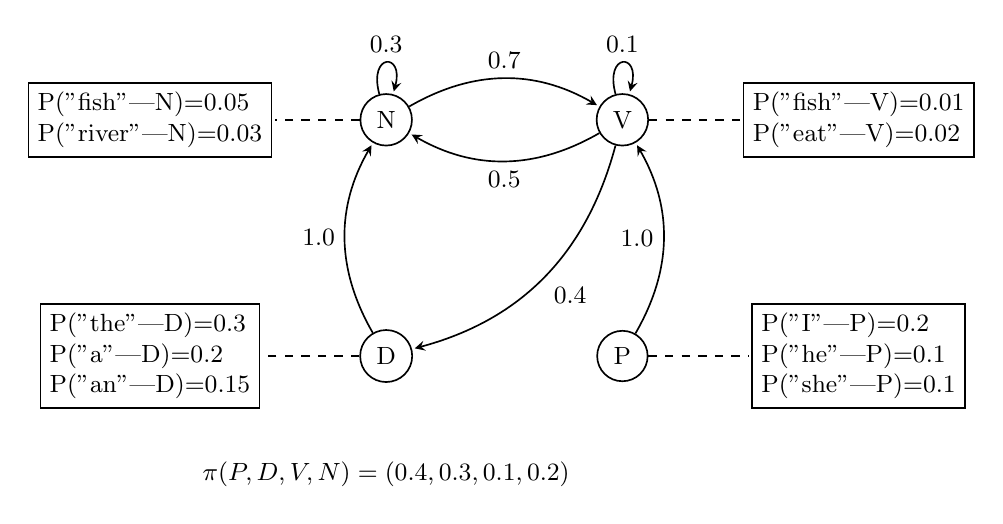
\begin{tikzpicture}[
	> = stealth, % arrow head style
	shorten > = 1pt, % don't touch arrow head to node
	auto,
	node distance = 3cm, % distance between nodes
	semithick, % line style
	font=\small
	]
	
	\tikzstyle{every state}=[
	draw = black,
	thick,
	fill = white,
	minimum size = 4mm
	]
	
	\node[circle,draw] (qN) {N};
	\node[align=left,draw] (qNe) [left of=qN] {P("fish"|N)=0.05\\P("river"|N)=0.03};
	\node[circle,draw] (qV) [right of=qN] {V};
	\node[align=left,draw] (qVe) [right of=qV] {P("fish"|V)=0.01\\P("eat"|V)=0.02};
	\node[circle,draw] (qD) [below of=qN] {D};
	\node[align=left,draw] (qDe) [left of=qD] {P("the"|D)=0.3\\P("a"|D)=0.2\\P("an"|D)=0.15};
	\node[circle,draw] (qP) [right of=qD] {P};
	\node[align=left,draw] (qPe) [right of=qP] {P("I"|P)=0.2\\P("he"|P)=0.1\\P("she"|P)=0.1};
	\node[] () [below of=qD, yshift=1.5cm] {$\pi(P, D, V, N) = (0.4, 0.3, 0.1, 0.2)$};
	
	
	\path[->] 	
	(qN) 	edge [loop above] node {0.3} ()
	edge [bend left] node {0.7} (qV)
	(qV) 	edge [loop above] node {0.1} ()
	edge [bend left] node {0.5} (qN)
	edge [bend left] node {0.4} (qD)
	(qD)	edge [bend left] node {1.0} (qN)
	(qP)	edge [bend right] node {1.0} (qV);
	
	\path[dashed] 	
	(qN) 	edge [] node {} (qNe)
	(qV) 	edge [] node {} (qVe)
	(qD) 	edge [] node {} (qDe)
	(qP) 	edge [] node {} (qPe);
	
	\end{tikzpicture}
	
	\begin{enumerate}
		\item Calculer les deux probabilités : P(V D N | ``fish a fish") et P(N D N | "fish a fish")
		\item Étant donné que C(N) = 200, C(V) = 100 et C(D)=100, calculer les probabilités suivantes en utilisant le lissage de Laplace : P(D|V), P(D|N) et P(N|D).
		\item Recalculer les probabilités de la première question après le lissage.
		\item Combien d'expressions étiquetées ``\textbf{V D N}" existent-elles dans notre dataset d'entraînement ? Le déterminant ``\textbf{D}" ne se produit jamais à la fin de la phrase. 
		
	\end{enumerate}
	
\end{enumerate}

\subsubsection*{Tutoriels}

Les tutoriels sont accessibles via le répertoire Github.
Dans le premier tutoriel, nous présentons la tâche d'étiquetage morpho-syntaxique avec NLTK qui est un outil implémenté en python destiné pour TALN.
Plusieurs algorithmes sont utilisés : RegEx, CRF, HMM, Perceptron et Brill.
Nous présentons, aussi, la tâche d'extraction des entités nommées et celle d'extraction des syntagmes nominaux.

Le deuxième tutoriel utilise flair ; un outil en python pour TALN.
Nous présentons les deux tâches : étiquetage morphosyntaxique et extraction des entités nommées.
Dans le tutoriel, nous pouvons apprendre comment utiliser un modèle existant et comment créer un nouveau modèle.

\subsubsection*{TP : Analyse morphosyntaxique}

On veut concevoir un petit programme pour l'analyse morphosyntaxique à partir de zéro. 
Le modèle HMM avec lissage de Laplace est fourni.
L'étudiant doit implémenter la méthode de décodage ``viterbi".

L'énoncé complet du TP ainsi que les codes et les données sont téléchargeables à partir du répertoire Github.
Le TP est implémenté complètement à partir de zéro (from scratch) : le module HMM et le module qui l'utilise pour l'analyse morphosyntaxique. 
L'étudiant doit compléter deux fonctions du premier module : notation ($p(t_i|t_{i-1}, w_i)$) et décodage viterbi.
Deux autres algorithmes de décodage sont implémentés : force brute et gourmand.
L'étudiant doit comparer entre les trois modèles en calculant la complexité en temps.
Les langages de programmation disponibles (pour l'instant) sont : Java, Javascript/nodejs et Python.

%\subsubsection*{Lab}
%
%Dans la tâche du "Jugements d'acceptabilité", on essaye de deviner si une phrase est acceptable grammaticalement. 
%Par exemple, l'expression "\textbf{Le livre qu'ont puisse trouvé sur internet ...}" ne peut pas être considérée comme acceptable. 
%La raison est que le verbe "ont (avoir)" est moins probable de suivre "que" et que le verbe "puisse (pouvoir)" est conjugué en présent subjonctif, or il est plus probable d'être en infinitif s'il suit le verbe "avoir".
%Dans ce lab, on va essayé de tester des différents modèles de langages afin d'accomplir cette tâche.
%
%L'énoncé complet du lab est téléchargeable à partir du répertoire Github.
%Les outils utilisés sont NLTK et Keras.

%=====================================================================
\ifx\wholebook\relax\else
% \cleardoublepage
% \bibliographystyle{../use/ESIbib}
% \bibliography{../bib/RATstat}
	\end{document}
\fi
%=====================================================================


% !TEX TS-program = xelatex
% !TeX program = xelatex
% !TEX encoding = UTF-8
% !TEX spellcheck = fr

%=====================================================================
\ifx\wholebook\relax\else
	\documentclass{KodeBook}
	% !TEX TS-program = xelatex
% !TeX program = xelatex
% !TEX encoding = UTF-8
% !TEX spellcheck = fr

%\usepackage[T1]{fontenc}

%\usepackage[pdftex]{graphicx}

%\usepackage{listingsutf8}
%\usepackage{xcolor}
%\usepackage{times}
\usepackage{array}
\usepackage{natbib}
\usepackage{lscape}%to flip tables in a page
\usepackage{pdflscape}
\usepackage{longtable}
\usepackage{tabu}
\usepackage{wrapfig}
\usepackage{colortbl}
\usepackage{alltt}
\usepackage[french,lined]{algorithm2e}

\renewcommand{\cite}[1]{\citep{#1}}

%\usepackage[english]{babel}

\bibliographystyle{engdnat}%unsrtnat, plainnat

%\usepackage{pgf-umlcd}





\hypersetup{
	pdfkeywords={TALN; TAL; langue},
	pdfsubject={intelligence artificielle; traitement automatique de langages naturels}
}

\renewcommand{\UrlFont}{\ttfamily\footnotesize}

\DeclareAcronym{taln}{
	short = TALN ,
	long  = traitement automatique de langages naturels,
	class = abbrev
}

\DeclareAcronym{tal}{
	short = TAL ,
	long  = traitement automatique des langues,
	class = abbrev
}


%\makeglossaries

%\newacronym{oop}{OOP}{Object-oriented programming} 

	\begin{document}
		\mainmatter
	
\fi
%=====================================================================
\changegraphpath{../img/syntaxe/}
\chapter{Analyse syntaxique}

\begin{introduction}[LES L\textcolor{white}{A}NGUES]
	\lettrine{A}{nalyser} un texte syntaxiquement veut dire mettre en évidence sa structure.
	Prenons la phase ``Much to learn, you still have." comme exemple d'analyse.
	Il est clair que le vocabulaire est d'origine anglaise, mais la phrase semble un peu étrange. 
	En anglais, les phrases sont souvent structurées comme sujet-verbe-objet. 
	Mais dans cette phrase, l'ordre est différent : objet-sujet-verbe ; une structure similaire aux langues amérindiennes d'Amazonie. 
	Bien sûr, dans ce cas c'est la syntaxe utilisée par Yoda (Star Wars).
	Il y a plusieurs façons de voir la structure syntaxique : une composition des structures jusqu'à arriver à une structure élémentaire, un ensemble de relations entre les mots, etc. 
	Dans ce chapitre, nous allons présenter deux structures syntaxiques ainsi que quelques méthodes d'analyse syntaxique pour les deux.
\end{introduction} 


La syntaxe étudie la manière dont les mots sont combinés afin de former une phrase.
Elle cherche à définir une structure standard des phrases d'un langage (naturel ou artificiel).
L'analyse syntaxique aide à décider si une phrase est grammaticalement correcte ou non. 
Si oui, nous essayons de trouver sa structure afin d'aider d'autres tâches comme :
\begin{itemize}
	\item Détection des erreurs grammaticales 
	\item Compréhension de la langue
	\item Extraction d'information 
\end{itemize}

%===================================================================================
\section{Structures syntaxiques}
%===================================================================================

Une langue doit avoir une structure syntaxique ; des règles qui aident la formation des phrases. 
Nous parlons ici d'une phrase grammaticalement correcte ; cela ne veut pas dire que la phrase doit avoir un sens. 
Donc, le fait qu'une phrase est bien formée syntaxiquement n'est pas une garantie qu'elle est sémantiquement correcte. 
Par exemple, la phrase ``\expword{Les idées vertes et non colorées dorment furieusement.}" est bien formée syntaxiquement, mais n'a aucun sens.
Il existe plusieurs théories pour représenter la structure syntaxique :
\begin{itemize}
	\item Grammaire générative et transformationnelle 
	\item Grammaire de dépendance 
	\item Grammaire catégorique
	\item Grammaires stochastiques
	\item Approches fonctionnelles de la grammaire
\end{itemize}

\subsection{Annotation constituante}

Nous avons vu dans le chapitre précédent que chaque mot d'une langue a une catégorie grammaticale (Ex. ``\expword{Le/DET cours/NOM est/VP intéressant/ADJ}"). 
Si nous revenions au chapitre des modèles de langage, nous pourrions déduire que le déterminant possède une grande probabilité d'être suivi par un nom ou un adjectif suivi par un nom (En RegEx : /\expword{DET ADJ* NOM}/). 
Nous appelons cette structure un \keyword[S]{syntagme} nominal. 
Il est appelé ``nominal" et pas ``adjectival" ou ``déterminant" puisque le nom ici est le centre de la structure. 
L'adjectif modifie souvent un nom et un déterminant est toujours dépendant d'un nom. 
Il existe plusieurs \keywordpl[S]{syntagme} selon la catégorie noyau : nominal, verbal, adjectival, prépositionnel, etc.
Par exemple, \expword{[Le/DET cours/NOM ]\textsubscript{NP} [est/V intéressant/ADJ VP]\textsubscript{VP}}.
La composition de plusieurs \keywordpl[S]{syntagme} forment un autre syntagme jusqu'à arriver à la phrase. 
Techniquement, une phrase peut être structurée comme un arbre où la racine est la phrase, les syntagmes sont représentés par des nœuds internes et les mots avec leurs catégories grammaticales sont représentés par des feuilles.

Rappelons la classification de Chomsky ; un langage peut être : régulier, hors-contexte, contextuel ou récursivement énumérable. 
Plusieurs langues peuvent être formalisées en utilisant une grammaires à contexte libre ; en anglais \acl{cfg}.
La grammaire $G <\Sigma, N, P, S>$ d'un langage est composée de :
\begin{itemize}
	\item $\Sigma$ : ensemble des symboles terminaux ; dans ce cas, le vocabulaire. 
	Exemple, \expword{$\Sigma$ = \{le, petit, chat, mange, un, poisson, ...\}}. 
	
	\item $N$ : ensemble des symboles non terminaux ; les variables (syntagmes et catégories grammaticales plus d'autres variables supplémentaires). 
	Par exemple, \expword{$N$ = \{S, NP, VP, DET, N, ADJ, ...\}}.
	
	\item $S \in N$ : axiome ; c'est le point de départ pour former la phrase. 
	
	\item $P$ : ensemble des règles de production.
	Les règles sont de la forme $A \rightarrow \beta \text{ avec } A \in N,\, \beta \in (\Sigma \cup N)^*$.
	Par exemple, \expword{P=\{S \textrightarrow\ NP VP, NP \textrightarrow\ DET ADJ N \textbar\ DET N, VP \textrightarrow\ V NP\}}
\end{itemize}

Parmi les problèmes trouvés lors de l'analyse syntaxique, l'ambigüité syntaxique.
Prenons, à titre d'exemple, la grammaire suivante (une grammaire pas bien définie) : 
\begin{itemize}
	\item S \textrightarrow\ NP VP (1)
	\item NP \textrightarrow\ DT NN (2) | DT NN PP (3)
	\item VP \textrightarrow\ VB NP (4) | VB NP PP (5)| VB PP (6) | AU VP (7)
	\item PP \textrightarrow\ PR NP (8)
	\item DT \textrightarrow\ l' | une | son 
	\item NN \textrightarrow\ élève | solution | stylo | explication 
	\item VB \textrightarrow\ écrit 
	\item AU \textrightarrow\ a
	\item PR \textrightarrow\ avec
\end{itemize}
Selon cette grammaire, la phrase ``\expword{L'élève a écrit une solution avec son explication}" aura deux interprétations. 
Les deux arbres syntaxiques sont illustrées dans la figure \ref{fig:cfg-ambigue}.
La première considère la préposition ``avec" dépendante du nom ``solution", et donc nous aurons la dérivation suivante (Figure \ref{fig:cfg-ambigue}(1)) : 
\begin{align*}
S & \sststile{}{(1)} NP\ VP \sststile{}{(2)} DT\ NN\ VP \sststile{}{(7)} DT\ NN\ AU\ VP \\
  & \sststile{}{(4)} DT\ NN\ AU\ VB\ NP \sststile{}{(3)} DT\ NN\ AU\ VB\ DT\ NN\ PP \\
  & \sststile{}{(8)} DT\ NN\ AU\ VB\ DT\ NN\ PR\ NP 
   \sststile{}{(2)} DT\ NN\ AU\ VB\ DT\ NN\ PR\ DT\ NN 
\end{align*}
La deuxième considère la préposition ``avec" dépendante du verbe ``écrit", et donc nous aurons la dérivation suivante (Figure \ref{fig:cfg-ambigue}(2)) :
\begin{align*}
S & \sststile{}{(1)} NP\ VP \sststile{}{(2)} DT\ NN\ VP \sststile{}{(7)} DT\ NN\ AU\ VP \\
& \sststile{}{(5)} DT\ NN\ AU\ VB\ NP\ PP \sststile{}{(2)} DT\ NN\ AU\ VB\ DT\ NN\ PP \\
& \sststile{}{(8)} DT\ NN\ AU\ VB\ DT\ NN\ PR\ NP 
 \sststile{}{(2)} DT\ NN\ AU\ VB\ DT\ NN\ PR\ DT\ NN 
\end{align*}
Clairement il y a une ambigüité ici ; donc, essayons de reformuler les deux dérivations.
La première veut dire : la solution et son explication ont été écrites par l'élève. 
La deuxième veut dire : la solution a été écrite par l'élève en utilisant l'explication de ce même élève.
Clairement, l'explication n'est pas un outil d'écriture ; donc la première est la plus juste. 
Afin de régler l'ambigüité, nous avons besoin du niveau sémantique qui peut guider l'analyse. 
Dans notre exemple, nous pouvons ajouter l'information que les outils d'écriture doivent être des entités concrètes et l'objet de l'écriture doit être un entité abstraite. 
\begin{figure}[ht]
	\begin{tabular}{cc}
		\hgraphpage[0.45\textwidth]{cfg-ambigue1.pdf} &
		\hgraphpage[0.45\textwidth]{cfg-ambigue2.pdf} \\
		(1) & (2) \\
	\end{tabular}
	\caption[Exemple de deux arbres syntaxiques d'une même phrase]{Exemple de deux arbres syntaxiques de la phrase ``L'élève a écrit une solution avec son explication" \label{fig:cfg-ambigue}}
\end{figure}

Une autre méthode pour faire face à ce problème est d'utiliser les \ac{cfg} probabilistes : \ac{pcfg}.
La grammaire est similaire à celle d'un \ac{cfg} : $G <\Sigma, N, P, S>$. 
La seule différence est que les règles sont de la forme : $A \rightarrow \beta\, [p] \text{ avec } A \in N,\, \beta \in (\Sigma \cup N)^*$.
Seulement, nous avons ajouté la probabilité $p$ d'occurrence de la règle. 
Afin d'estimer cette probabilité, nous utilisons un corpus annoté (\keyword[T]{TreeBank}). 
Étant donné la fonction $C$ qui calcule le nombre d'occurrence, la probabilité d'une règle $A \rightarrow \beta$ est estimée en utilisant l'équation \ref{eq:pcfg-est}.
Dans le cas d'ambigüité entre plusieurs règles, nous choisissons celle avec le maximum de probabilité.
\begin{equation}\label{eq:pcfg-est}
	P(A \rightarrow \beta | A) = \frac{C(A \rightarrow \beta)}{C(A)}
\end{equation}


\subsection{Annotation fonctionnelle}

Un mot ou plus remplissent une fonction syntaxique (Ex. \expword{sujet, objet, etc.}).
Par exemple, dans la phrase ``\expword{Le chat mange un poisson}", le mot ``chat" est le sujet du verbe ``mange". 
Dans l'annotation fonctionnelle, la fonction syntaxique est une relation binaire appelée \keyword{dépendance}.
Une relation de dépendance relie un mot appelé \keyword{tête syntaxique} avec un autre appelé \keyword{dépendant}. 
Un mot ne peut être un dépendant qu'une seule fois, mais il peut être une tête syntaxique plusieurs fois. 
Un exemple de l'annotation fonctionnelle des deux phrases ``\expword{L'élève a écrit une solution et son explication}" et ``\expword{L'élève a écrit une solution avec son stylo}" est illustré dans la figure \ref{fig:parse-fct-exp}.
%
\begin{figure}[ht]
	\centering
	\hgraphpage[0.65\textwidth]{exp-parse-fonct_.pdf}
	\caption[Exemple d'une analyse fonctionnelle de deux phrases]{Exemple d'une analyse fonctionnelle de deux phrases en utilisant \url{https://corenlp.run/} [visité le 2021-09-25]\label{fig:parse-fct-exp}}
\end{figure}

La structure de dépendance est formalisée comme un graphe orienté $G=(V, A)$ où les mots sont représentés par des sommets $V$ et les relations sont représentées par des arcs $A$. 
L'arbre de dépendances d'une phrase satisfait les conditions suivantes : 
\begin{itemize}
	\item Il existe un seul nœud racine désigné qui n'a pas d'arcs entrants. En général c'est un verbe.
	\item À l'exception du nœud racine, chaque sommet a exactement un arc entrant.
	\item Il existe un chemin unique du nœud racine à chaque sommet de $V$.
\end{itemize}

Les relations de dépendance sont des relations entre deux entités. 
Un exemple des relations de dépendance est donnée dans le tableau \ref{tab:rel-dep-exp}.
\begin{table}[ht]
	\begin{tabular}{p{.2\textwidth}p{.35\textwidth}p{.35\textwidth}}
		\hline\hline
		\textbf{Dép. de base} & \textbf{Description} & \textbf{Exemple}\\
		\hline
		nsubj & sujet nominal & \expword{Le \underline{people} \textbf{gagne}}\\
		obj & objet direct & \expword{On \textbf{présente} le \underline{cours}}\\
		iobj & objet indirect & \expword{Il \underline{m'}\textbf{envoie}}\\
		csubj & sujet propositionnel & \expword{\underline{Suivre} le cours \textbf{permet} ...}\\
		&&\\
		\hline\hline
		\textbf{Dép. des noms} & \textbf{Description} & \textbf{Exemple}\\
		\hline
		amod & modificateur adjectival & \expword{La \textbf{fille} \underline{modeste}}\\
		det & déterminant & \expword{\underline{La} \textbf{fille}}\\
		nmod & modificateur nominal & \expword{Le \underline{résultat} de la \textbf{course}}\\
		nummod & modificateur numérique & \expword{J'ai mangé \underline{3} \textbf{bonbons}}\\
		\hline\hline
	\end{tabular}
	\caption[Quelques relations de dépendances universelles de Stanford]{Quelques relations de dépendances universelles de Stanford \cite{2014-de-marneffe-al}, \url{https://universaldependencies.org/u/dep/index.html} [visité le 2021-09-11] }
	\label{tab:rel-dep-exp}
\end{table}

%===================================================================================
\section{Analyse des constituants}
%===================================================================================

La grammaire à contexte libre est le système formel le plus utilisé pour modéliser la structure constituante.
Il existe deux types de méthodes pour analyser un texte :
\begin{itemize}
	\item \optword{ascendante} : à partir des mots de la phrase, nous essayons de trouver les catégories grammaticales. Ensuite, les syntagmes qui génèrent une combinaison des catégories et des \keywordpl[S]{syntagme}. 
	Nous fusionnons les syntagmes jusqu'à arriver à l'axiome ``S".
	Exemple, \expword{LR}.
	\item \optword{descendante} : à partir de l'axiome ``S", nous cherchons les règles qui génèrent la phrase. 
	Dans cette approche, nous nous basons sur les mots pour guider la génération.
	Exemple, \expword{Descente récursive, LL, Early}.
\end{itemize}
Les algorithmes mentionnées dans les exemples sont conçus pour traiter les langages de programmation. 
Ces derniers ont des syntaxes bien définies qui peuvent être traitées d'une manière déterministe. 
Les langages naturels contiennent beaucoup d'ambigüité et les règles sont plus complexes. 
Un algorithme conçu pour l'analyse syntaxique des langages naturels est \keyword[C]{CKY}.

\subsection{Algorithme CKY}

L'algorithme de \keyword{Cocke-Kasami-Younger} (\keyword[C]{CKY}) utilise la programmation dynamique afin d'appliquer une analyse syntaxique ascendante. 
La seule condition pour appliquer cet algorithme est de transformer la grammaire $G <\Sigma, N, P, S>$ sous la forme normale de Chomsky. 
Un petit rappel de cette forme ($N$ est l'ensemble des variables et $\Sigma$ est le vocabulaire): 
\begin{align*}
	A & \rightarrow  B C \text{ où } A, B, C \in N\\
	A & \rightarrow w \text{ où } w \in \Sigma
\end{align*}


Après transformation de la grammaire $G <\Sigma, N, P, S>$ sous FNC, nous pouvons l'utiliser pour la reconnaissance des phrases. 
Étant donné une phrase $w = w_1 \ldots w_n$, nous créons un tableau triangulaire $T$ de taille $n*n/2$. 
L'algorithme \ref{algo:cky-recon} décrit comment remplir ce tableau afin d'analyser le mot $w$ suivant la grammaire $G$ en FNC. 
Je l'ai modifié un peu pour pouvoir revenir en arrière et créer l'arbre syntaxique : chaque cellule contient un ensemble des quadruplets (variable, index des fils, position du 1ier fils, position du deuxième fils).
L'algorithme prend un temps $O(n^3 * |P|)$ où $P$ est l'ensemble des productions.
Nous commençons par remplir le diagonal du tableau $T$ par les variables $A$ qui génèrent les mots $w_i$ de la phrase $w$ ($A \rightarrow\ w_i$). 
Nous continuons le remplissage du bas vers le haut et du gauche vers le droit. 
Chaque cellule est remplie par une variable qui génère une des variables à gauche (colonne $k$) suivie par une des variables en bas (ligne $k$) où $i \le k \le j$.
Lorsque nous arrivons à la dernière cellule de la première ligne, nous devons trouver l'axiome ``S" ; sinon, la phrase n'appartient pas au langage.
%\begin{algorithm}[ht]
%	\Donnees{une grammaire $G <\Sigma, N, P, S>$ en FNC; une phrase $w = w_1 \ldots w_n$}
%	\Res{$T[n, n], B[n, n, |N|]$}
%	
%	\Pour{$ i = 1 \ldots n$}{ %\tcc*{Iitialiser le diagonal}
%		$T[i, i] \leftarrow \{  A / (A \rightarrow w_i) \in P \} $\;
%	}
%	
%	\Pour{$ j = 2 \ldots n$ }{
%		\Pour{$ i = 0 \ldots (n - j) $}{
%			\Pour{$ k = (i+1) \ldots (i + j -1 ) $}{
%				\PourTous{$A$ tel que $(A \rightarrow B C) \in P $ et $B \in T[i, k]$ et $C \in T[k, i+j]$}{ 
%					$T[i, i+j] \leftarrow T[i, i+j] \cup \{A\}$ \;
%					$B[i, i+j, A] \leftarrow B[i, i+j, A] \cup \{(B, C, k)\}$ \;
%				}
%			}
%		}
%	}
%	
%	\Si{$``S" \notin T[0, n] $} {
%		Erreur ``La phrase n'a pas été reconnue"\;
%	}
%	
%	\Retour $T, B$ \;
%	\caption{Reconnaissance d'une phrase en utilisant la méthode CKY}
%	\label{algo:cky-recon}
%\end{algorithm}
\begin{algorithm}[ht]
	\Donnees{une grammaire $G <\Sigma, N, P, S>$ en FNC; une phrase $w = w_1 \ldots w_n$}
	\Res{$T[n, n]$}
	
	\Pour{$ i = 1 \ldots n$}{ %\tcc*{Initialiser le diagonal}
		$T[i, i] \leftarrow \{ (A, 0, 0, 0) / (A \rightarrow w_i) \in P \} $\;
	}
	
	\Pour{$ i = (n-1) \ldots 1$ }{
		\Pour{$ j = (i+1) \ldots n $}{
			\Pour{$ k = i \ldots (j-1) $}{
				\PourTous{$A$ tel que $(A \rightarrow B C) \in P $ et $B \in T[i, k]$ et $C \in T[k+1, j]$}{
					$iB \leftarrow index(B, T[i, k])$ \;
					$iC \leftarrow index(C, T[k+1, j])$ \;
					$T[i, j] \leftarrow T[i, j] \cup \{(A, k, iB, iC)\}$ \;
				}
			}
		}
	}
	
	\Si{$``S" \notin T[1, n] $} {
		Erreur ``La phrase n'a pas été reconnue"\;
	}
	
	\caption{Reconnaissance d'une phrase en utilisant la méthode CKY}
	\label{algo:cky-recon}
\end{algorithm}

Une fois la phrase $w$ acceptée et le tableau rempli, nous utilisons ce denier pour générer l'arbre syntaxique. 
Nous commençons par choisir les deux fils de l'axiome $S$ en se basant sur $T$.
Nous cherchons les fils de chaque nœud récursivement jusqu'à arriver à un nœud sans fils.
L'algorithme \ref{algo:cky-constr} décrit l'opération de construction d'un arbre syntaxique en détail.
\begin{algorithm}[ht]
	\SetKwFunction{FConst}{Construire}
	\SetKwProg{Fn}{Fonction}{\\Début}{Fin}
	
	\Donnees{$T[n, n]$}
	\Res{Racine de l'arbre syntaxique : $r \leftarrow \varnothing$}
	
	\Si{$``S" \in T[1, n] $} {
		$r \leftarrow $ \FConst{$1, n, index(``S", T[1, n])$}\;
	}
	
	\Fn{\FConst{$i, j, pos$}}{
		$ (A, k, iB, iC) \leftarrow T[i, j][pos] $\;
		Créer un nouveau nœud : nœud\;
		nœud.valeur $\leftarrow  A$ \;
		\Si{$k>0$}{
			nœud.gauche $\leftarrow$ \FConst{$i, k, iB$}\;
			nœud.droit $\leftarrow$ \FConst{$k+1, j, iC$}\;
		}
		\Retour nœud\;
	}
	
	\caption{Construction de l'arbre syntaxique en utilisant CKY}
	\label{algo:cky-constr}
\end{algorithm}
%
%\begin{algorithm}[ht]
%	\SetKwFunction{FConst}{Construire}
%	\SetKwProg{Fn}{Fonction}{\\Début}{Fin}
%	
%	\Donnees{$T[n, n], B[n, n, |N|]$}
%	\Res{Arbre syntaxique}
%	
%	\eSi{$``S" \notin T[0, n] $} {
%		\Retour $\varnothing$ \;
%	}{
%		\Retour \FConst{$S, 0, n$}\;
%	}
%	
%	\Fn{\FConst{$A, i, j$}}{
%		
%		\eSi{j = i + 1}{
%			\Retour $A$\;
%		}{
%			$ (B, C, k) \leftarrow Choisir(B[i, j, A]) $\;
%			\Retour (\FConst{$B, i, k$}, \FConst{$C, k, j$})\;
%		}
%	}
%	
%	
%	\caption{Construction de l'arbre syntaxique en utilisant CKY}
%	\label{algo:cky-constr}
%\end{algorithm}

L'arbre syntaxique résultant est binaire (à cause de la forme normale de Chomsky).
Mais, dans la réalité il doit suivre la grammaire conçue par les syntacticiens. 
Une solution est d'ajouter une étape de post-traitement pour récupérer l'arbre original.
Concernant les productions unitaires, nous pouvons les laisser telles qu'elles sont et modifier l'algorithme \keyword[C]{CKY} afin de les accepter.
Bien sûr l'algorithme souffre toujours du problème d'ambigüité syntaxique.
Exemple, ``\expword{Je mange du riz avec une fourchette}" et ``\expword{Je mange du riz avec de la viande}".

Nous allons analyser la phrase ``\expword{la petite forme une petite phrase}" en utilisant \keyword[C]{CKY} selon la grammaire suivante :
\begin{itemize}
	\item S \textrightarrow\ NP VP | VP
	\item VP \textrightarrow V NP
	\item NP \textrightarrow\ \textbf{DET ADJ N} \textbar\ DET N \textbar\ PRON 
	\item PRON \textrightarrow\ je \textbar\ tu \textbar\ il \textbar\ elle
	\item V \textrightarrow\ forme \textbar\ veut \textbar\ mange 
	\item DET \textrightarrow\ un \textbar\ une \textbar\ la \textbar\ le
	\item ADJ \textrightarrow\ petite \textbar\ grand \textbar\ bleu 
	\item N \textrightarrow\ petite \textbar\ forme \textbar\ phrase \textbar\ chat \textbar\ poisson
\end{itemize}
Nous transformons cette grammaire en FNC en remplaçant la règle en gras par : 
\begin{itemize}
	\item NP \textrightarrow\ DET AP
	\item AP \textrightarrow\ ADJ N
\end{itemize}
La règle unitaire $S \textrightarrow\ VP$ sera remplacée par $S \textrightarrow\ V NP$.
Le tableau d'analyse est illustré dans la figure \ref{fig:exp-cky-trait}.

\begin{figure}[ht]
\begin{tabular}{|p{2.3cm}|p{2.5cm}|p{2.3cm}|p{2.3cm}|p{2.5cm}|p{2.2cm}|}
	\hline
	la & petite & forme & une & petite & phrase \\
	\hline
	\textbf{(DET, 0, 0, 0)} & \textbf{(NP, 1, 1, 1)} & - & - & - & \textbf{(S, 2, 1, 1)} \\
	\hline
	\multicolumn{1}{l|}{}& \textbf{(ADJ, 0, 0, 0)}; (N, 0, 0, 0) & (AP, 2, 1, 2) & - & - & - \\
	\cline{2-6}
	\multicolumn{2}{l|}{}& \textbf{(V, 0, 0, 0)}; (N, 0, 0, 0) & - & (VP, 3, 1, 1) & \textbf{(VP, 3, 1, 1)}; (S, 3, 1, 1) \\
	\cline{3-6}
	\multicolumn{3}{l|}{}& \textbf{(DET, 0, 0, 0)} & (NP, 4, 1, 2) & \textbf{(NP, 4, 1, 1)} \\
	\cline{4-6}
	\multicolumn{4}{l|}{}& \textbf{(ADJ, 0, 0, 0)}; (N, 0, 0, 0) & \textbf{(AP, 5, 1, 1)} \\
	\cline{5-6}
	\multicolumn{5}{l|}{}& \textbf{(N, 0, 0, 0)} \\
	\cline{6-6}
\end{tabular}
\caption[Exemple de l'analyse CKY]{Exemple de l'analyse CKY de la phrase ``la petite forme une petite phrase" \label{fig:exp-cky-trait}}
\end{figure}


\subsection{Algorithme CKY probabiliste}

Dans l'algorithme \keyword[C]{CKY}, nous pouvons tomber sur un cas où nous avons plus d'un arbre syntaxique. 
Pour guider le choix des règles, nous ajoutons la probabilité de chaque production ; utilise une \ac{pcfg}.
Lors de la transformation d'une grammaire probabiliste $G<\Sigma, N, P, S>$ en FNC, les nouvelles règles créées par transformation en FNC ont une probabilité égale à $1$.
Étant donné un arbre syntaxique $T$ du mot $w$, sa probabilité est estimée selon l'équation \ref{eq:pcfg-arbre-prop}.
\begin{equation}
P(T, w) = \prod\limits_{(A_i \rightarrow \beta_i) \in T} P(A_i \rightarrow \beta_i)
\label{eq:pcfg-arbre-prop}
\end{equation}
L'arbre syntaxique le plus adéquat pour analyser le mot $w$ est celui avec le maximum de probabilité (voir \ref{eq:pcfg-arbre-max}).
\begin{equation}
\hat{T}(w) = \arg\max\limits_{T(w)} P(T, w)
\label{eq:pcfg-arbre-max}
\end{equation}

Concernant l'algorithme \keyword[C]{CKY}, nous ajoutons la probabilité d'occurrence d'une règle dans chaque cellule. 
Chaque variable $A$ aura au maximum une chance pour produire deux variables.
Dans ce cas, nous créons un tableau triangulaire de trois dimensions $T[n, n, |N|]$ où nous stockons la probabilité de chaque variable dans cette cellule en plus de la position $k$ utilisée pour chercher les fils et les deux variables des fils gauche et droit.
Nous supposons que toutes les probabilités des cellules soient initialisées à $0$.
L'algorithme \ref{algo:cky-prob-recon} représente la version probabiliste de l'algorithme \keyword[C]{CKY}.
\begin{algorithm}[ht]
	\Donnees{une grammaire $G <\Sigma, N, P, S>$ en FNC; une phrase $w = w_1 \ldots w_n$}
	\Res{$T[n, n, |N|]$}
	
	\Pour{$ i = 1 \ldots n$}{ %\tcc*{Initialiser le diagonal}
		$T[i, i, A] \leftarrow \{ (P(A \rightarrow w_i), 0, A, A) / (A \rightarrow w_i) \in P \} $\;
	}
	
	\Pour{$ i = (n-1) \ldots 1$ }{
		\Pour{$ j = (i+1) \ldots n $}{
			\Pour{$ k = i \ldots (j-1) $}{
				\PourTous{$A$ tel que $(A \rightarrow B C) \in P $ et $T[i, k, B] > 0$ et $T[k+1, j, C] > 0$}{
					$p \rightarrow P(A \rightarrow B C) * T[i, k, B][1] * T[k+1, j, C][1]$\;
					\Si{$p > T[i, j, A][1]$}{
						$T[i, j, A] \leftarrow (p, k, B, C)$ \;
					}
				}
			}
		}
	}
	
	\Si{$T[1, n, S] = 0 $} {
		Erreur ``La phrase n'a pas été reconnue"\;
	}
	
	\caption{Reconnaissance d'une phrase en utilisant la méthode CKY probabiliste}
	\label{algo:cky-prob-recon}
\end{algorithm}
%\begin{algorithm}[ht]
%	\Donnees{une grammaire probabiliste $G <\Sigma, N, P, S>$ en FNC; une phrase $w = w_1 \ldots w_n$}
%	\Res{$T[n, n, |N|], B[n, n, |N|]$}
%	
%	\Pour{$ i = 1 \ldots n$}{ 
%		\PourTous{$A / (A \rightarrow w_j) \in P$}{
%			$T[i-1, j, A] \leftarrow P(A \rightarrow w_j)$\;
%		}
%	}
%	
%	\Pour{$ j = 2 \ldots n$ }{%\tcc*{Iitialiser le diagonal}
%		\Pour{$ i = 0 \ldots (n - j) $}{
%			\Pour{$ k = (i+1) \ldots (i + j -1 ) $}{
%				%					\PourTous{$A$ tel que $(A \rightarrow B C) \in P $ et $B \in T[i, k]$ et $C \in T[k, i+j]$}{ 
%				$T[i, i+j, A] \leftarrow \max\limits_{A \rightarrow B C \in P} P(A \rightarrow B C) * T[i, k, B] * T[k, i+j, C]$ \;
%				$B[i, i+j, A] \leftarrow (B, C, k)$\;
%				%					}
%			}
%		}
%	}
%	
%	\texttt{// Si $``S" \notin T[0, n] $ : Erreur}
%	%		\Si{} {
%	%			Erreur ``La phrase n'a pas été reconnue"\;
%	%		}
%	
%	\Retour $T, B$ \;
%	\caption{CKY probabiliste : Reconnaissance d'une phrase}
%\end{algorithm}

%===================================================================================
\section{Analyse de dépendances}
%===================================================================================

Les dépendances syntaxiques sont des relations binaires entre deux mots. 
L'analyse des dépendances sert à trouver ces relations et créer un arbre syntaxique. 
Dans cet arbre, tous les nœuds sont des mots et chaque arc est une relation.
Nous allons présenter deux approches pour analyser les dépendances : par transitions et par graphes.

\subsection{Par transition}

Un analyseur des dépendances par transition peut être implémenté en utilisant la méthode SHIFT-REDUCE. 
C'est une machine abstraite ayant la configuration $C = (\sigma, \beta, A)$ (voir la figure \ref{fig:dep-trans-arch}) où :
\begin{itemize}
	\item $\sigma$ est une pile
	\item $\beta$ est le tampon (buffer) d'entrée. 
	Il contient le mot en entrée avec une tête qui pointe sur le mot courant.
	\item $A$ est la liste des arcs créés (dépendances)
\end{itemize}
L'analyse commence avec la configuration $C_{initiale} = ([ROOT], w, \emptyset)$ et termine avec la configuration $C_{finale} = ([ROOT], \varnothing, A)$.
Si nous arrivions à la fin du mot avec une pile non vide (on considère le sommet $ROOT$ comme vide) sans actions de vidage, nous pourrions conclure que ce mot n'appartient pas au langage. 
Une transition d'un état vers un autre peut être une action sur :
\begin{itemize}
	\item $\sigma$ : empiler ou dépiler un mot
	\item $\beta$ : retirer un mot ou ajouter un au début
	\item $A$ : ajouter une dépendance entre 2 mots
\end{itemize}
\textbf{Oracle} est un système qui décide la transition suivante.

\begin{figure}[ht]
	\centering
	\hgraphpage[.38\textwidth]{transitions.pdf}
	\caption{Architecture d'un analyseur des dépendances par transition \label{fig:dep-trans-arch}}
\end{figure}


Afin de décrire l'algorithme d'analyse, nous utilisons deux fonctions : ``$Oracle$" qui choisit une transition ``$t$", et ``$Appliquer$" qui exécute ``$t$" sur la configuration. 
L'algorithme \ref{algo:anal-dep-trans} décrit l'analyse des dépendances par transitions.

\begin{algorithm}[ht]
	\Donnees{Le mot à analyser $w= w_1 w_2 \ldots w_n$}
	\Res{Liste des dépendances $A$}
	
	$C \leftarrow (\sigma=[ROOT], \beta = w, A = \emptyset)$\;
	
	
	\Tq{$\sigma \ne [ROOT]$ OU $\beta \ne \varnothing$}{
		$t \leftarrow Oracle(C)$\;
		$C \leftarrow Appliquer(C, t)$\;
	}
	
	\caption{Analyse des dépendances par transitions \label{algo:anal-dep-trans}}
\end{algorithm}

Le système ``Oracle" choisit la transition suivante $\hat{t}$ parmi l'ensemble des transitions possibles $T$.
Lorsque nous sommes dans la configuration actuelle $ C = (\sigma, \beta, A) $, nous utilisons une fonction $\Psi$ qui calcule un score en utilisant des caractéristiques basées sur cette configuration.
La transition $\hat{t}$ choisie est celle qui maximise la fonction $\Psi$ ayant des paramètres $\theta$ selon l'équation \ref{eq:orancle-psi}.
\begin{equation}\label{eq:orancle-psi}
\hat{t} = \arg\max\limits_{t \in T} \Psi (t, C, w; \theta)
\end{equation}
Pour entraîner le système ``Oracle", nous devons annoter le texte en le transformant à une séquence de transitions. 
Le texte original est annoté avec les relations de dépendance. 
Pour transformer la sortie à une séquence de transitions, nous utilisons le système d'analyse en tel sorte à générer toutes les dépendances possibles. 
En utilisant des caractéristiques sur la configuration courante, nous essayons d'estimer la transition suivante par la fonction $\Psi$.  
Cette fonction peut être MaxEnt (la plus utilisée), SVM ou des réseaux de neurones. 
Les caractéristiques utilisées par la fonction $\Psi$ peuvent être des caractéristiques sur :  
\begin{itemize}
	\item la pile $\sigma$ : le mot dans le sommet de la pile et sa catégorie grammaticale. 
	\item le tampon d'entrée $\beta$ : les trois premiers mots et leurs catégories grammaticales.
	\item la liste des dépendances $A$ : les dépendances qui ont été estimées.
	\item la phrase analysée $w$ : la distance entre le mot du sommet de la pile et le premier mot dans le tampon (nombre des mots entre eux dans la phrase $w$)
\end{itemize}

Il y a deux approches pour l'analyse de dépendances par transitions : Arc-standard et Arc-eager. 
Dans Arc-standard, les relations de dépendances sont détectées seulement entre les mots dans la pile. 
Lorsqu'un mot est considéré comme une tête d'une relation, il sera éliminé de la pile. 
La figure \ref{fig:arc-standard-exp} représente un exemple d'analyse de la phrase ``\expword{they like bagels with lox}" en utilisant Arc-standard.
Les transitions possibles dans cette approche sont :
\begin{itemize}
	\item \optword{SHIFT} : déplacer le premier élément dans le tampon vers la pile 
	\[ (\sigma, w_i|\beta, A) \Rightarrow  (\sigma|w_i, \beta, A) \]
	
	\item \optword{ARC-LEFT} : établir un arc du premier élément dans le tampon vers le sommet de la pile
	\[ (\sigma|w_i, w_j|\beta, A) \Rightarrow  (\sigma, w_j|\beta, A \cup \{w_j \rightarrow w_i \}) \] 
	
	\item \optword{ARC-RIGHT} : établir un arc du sommet de la pile vers le premier élément dans le tampon
	\[ (\sigma|w_i, w_j|\beta, A) \Rightarrow  (\sigma, w_i|\beta, A \cup \{w_i \rightarrow w_j \}) \] 
\end{itemize}

\begin{figure}[ht]
	\centering
	\hgraphpage[.8\textwidth]{exp-arc-std_.pdf}
	\caption[Exemple de dérivations non étiquetées en utilisant Arc-standard]{Exemple de dérivations non étiquetées de la phrase ``\expword{they like bagels with lox}" en utilisant Arc-standard \cite{2018-eisenstein}\label{fig:arc-standard-exp}}
\end{figure}

Dans Arc-Eager, nous essayons de détecter les relations de dépendance le plus tôt possible. 
Pour ce faire, les relations doivent être détectées entre le sommet de la pile et le mot courant. 
Dans ce cas, nous n'avançons pas la tête de lecture automatiquement lorsque nous ajoutons une nouvelle relation. 
Dans ce cas, la seule méthode pour le faire est d'empiler le mot dans la pile en utilisant la transition ``SHIFT". 
Un exemple de l'analyse de la phrase ``\expword{they like bagels with lox}" en utilisant Arc-eager est illustré dans la figure \ref{fig:arc-eager-exp}.
Les transitions possibles dans cette approches sont :
\begin{itemize}
	\item \optword{SHIFT} est le même que ``Arc-standard"
	
	\item \optword{ARC-LEFT} : établir un arc du premier élément dans le tampon vers le sommet de la pile
	\[ (\sigma|w_i, w_j|\beta, A) \xRightarrow{\forall w_k (w_k \rightarrow w_i) \notin A}  (\sigma, w_j|\beta, A \cup \{w_j \rightarrow w_i \}) \] 
	
	\item \optword{ARC-RIGHT} : établir un arc du sommet de la pile vers le premier élément dans le tampon
	\[ (\sigma|w_i, w_j|\beta, A) \Rightarrow  (\sigma|w_i w_j, \beta, A \cup \{w_i \rightarrow w_j \}) \] 
	
	\item \optword{REDUCE} : dépiler un mot s'il a déjà un parent
	\[ (\sigma|w_i, \beta, A) \xRightarrow{\exists w_k (w_k \rightarrow w_i) \in A} (\sigma, \beta, A) \] 
	%	\[ (\sigma|w_i, \beta, \mathcal{A}) \overset{\exists w_k (w_k \rightarrow w_i) \in \mathcal{A}}{\Longrightarrow} (\sigma, \beta, \mathcal{A}) \] 
\end{itemize}

\begin{figure}[ht]
	\centering
	\hgraphpage[.8\textwidth]{exp-arc-eager_.pdf}
	\caption[Exemple de dérivations non étiquetées en utilisant Arc-eager]{Exemple de dérivations non étiquetées de la phrase ``\expword{they like bagels with lox}" en utilisant Arc-eager \cite{2018-eisenstein}\label{fig:arc-eager-exp}}
\end{figure}

Les relations présentées ici sont des relations non étiquetées ; juste la relation tête-dépendant sans type.
Afin d'ajouter le type de la relation, nous devons enrichir les transitions ``ARC-LEFT" et ``ARC-RIGHT" avec les types possibles. 
Dans Arc-standard, à la place de 3 transitions, nous aurons $1+2R$ transitions où $R$ est le nombre des types de dépendances.

\subsection{Par graphe}

Le filtrage des relations non probables est une autre approche pour trouver l'arbre de dépendance d'un mot donné $w$. 
Dans un premier temps, nous considérons toutes les dépendances possibles entre les mots. 
Ensuite, nous commençons à éliminer les relations non probables jusqu'à arriver au résultat final. 
D'une façon plus formelle, nous commençons l'analyse par un graphe complet $G = (V, E)$ où $V$ est l'ensemble de nœuds (mots) et $E$ l'ensemble d'arcs (relations de dépendance). 
Ensuite, nous cherchons l'arbre $T = (V, F)$ parmi les arbres possibles $\mathcal{T}(G)$ qui est un sous-graphe de $G$ maximisant un certain score comme indiqué dans l'équation \ref{eq:arbre-rela-max}.
\begin{equation}
\hat{T} = \arg\max\limits_{T \in \mathcal{T}(G)} \Psi(T, w; \theta)
\label{eq:arbre-rela-max}
\end{equation}
Le score $\Psi$ d'un arbre $T$ est la somme des scores $\psi$ de ces arcs (voir l'équation \ref{eq:arbre-rela-score}). 
$\theta$ est l'ensemble des paramètres utilisés dans la fonction du score.
\begin{equation}
\Psi(T, w; \theta) = \sum_{e \in F / T = (V, F)} \psi(e, w; \theta)
\label{eq:arbre-rela-score}
\end{equation}

\begin{figure}[ht]
	\centering
	\hgraphpage[.38\textwidth]{graphe.pdf}
	\caption{Architecture d'un analyseur des dépendances par graphe \label{fig:dep-graph-arch}}
\end{figure}

Afin d'estimer le score d'un arc $e$, nous pouvons utiliser un certain nombre de caractéristiques $f$ comme : le mot de l'entête, sa catégorie grammaticale, son lemme, ses préfixes et suffixes, la direction de l'arc, la distance entre l'entête et le dépendant, etc.
Un algorithme d'apprentissage ayant les paramètres $\theta$ est utilisé pour apprendre à estimer le score d'un arc $e$ selon ces caractéristiques. 
En utilisant des scores initiaux, nous générons un arbre et nous le comparons avec l'arbre destinataire. 
Si les arbres ne soient pas identiques, nous calculerions l'erreur et nous mettrions à jours les paramètres.
Le score d'un arc $e$ est représenté par l'équation \ref{eq:arbre-rela-score2}.
\begin{equation}
\psi(e, w; \theta) = \sum_{k = 1}^{K} \theta_k f_k(e, w)
\label{eq:arbre-rela-score2}
\end{equation}


Afin de créer un arbre à partir d'un graphe, nous pouvons utiliser l'algorithme de Chu-Liu/Edmonds (voir l'algorithme \ref{algo:chu-liu-edmonds}).
Pour analyser un mot $w=w_1 \ldots w_n$, nous commençons par construire un graphe complet $G = (V, E)$ où chaque nœud $v_i$ représente un mot $w_i$ et chaque arc $e$ représente une relation possible entre deux nœuds. 
Afin de représenter l'information du mot racine, nous ajoutons un nœud (ROOT) avec des arcs vers tous le reste des nœuds.
Pour chaque arc $e$ du graphe $G$, nous affectons un poids $G.p(e)$ qui est estimé en utilisant l'apprentissage automatique.
En prenant le nœud ``ROOT" comme racine et le graphe $G$, nous essayons de trouver un arbre $T = (V, F)$ couvrant de poids maximal. 
Un arbre couvrant est un sous-graphe acyclique maximal où tous les nœuds sont connectés et il n'y a plus qu'un arc entrant vers un nœud.
Deux fonctions sont utilisées dans cette algorithme :
\begin{itemize}
	\item \optword{Contracter} : une fonction qui fusionne deux nœuds $u$ et $v$ composant un cycle $C$
	\begin{itemize}
		\item $\forall e = (u', v) \in E : G.p(e) \leftarrow G.p(e) - G.p((u, v)) $
		\item $\forall e = (v', u) \in E : G.p(e) \leftarrow G.p(e) - G.p((v, u)) $
	\end{itemize}
	\item \optword{Etendre} : une fonction qui désassemble les deux nœuds $u$ et $v$ d'un cycle $C$. L'arc qui enfreint la condition ``\textit{pas de deux arcs entrants}" est supprimé.
\end{itemize}

\begin{algorithm}[ht]
	\Donnees{un graphe pondéré $G = (V, E)$, $ ROOT $}
	\Res{un arbre couvrant $T = (V, F)$}
	
	\SetKwFunction{ACM}{ArbreCouvrantMax}
	\SetKwProg{Fn}{Fonction}{}{Fin Fonction} 
	
	\Fn{\ACM{$G, ROOT$}}{
		
		$F \leftarrow \emptyset$\;
		
		\PourTous{$ v \in V$}{ 
			$meilleurInArc \leftarrow \arg\max_{e = (u, v) \in E} G.p(e) $;
			$F \leftarrow F \cup meilleurInArc$\;
			\PourTous{$e = (u, v) \in E$}{ 
				$ G.p(e) \leftarrow G.p(e) - G.p(meilleurInArc) $\;
			}
			\eSi{$T = (V, F)$ est un arbre couvrant}{
				\Retour $T$ \;
			}{
				$C \leftarrow$ un cycle de $F$;
				$G' \leftarrow Contracter(G, C)$\;
				$T' \leftarrow ArbreCouvrantMax(G', ROOT)$;
				$T \leftarrow Etendre(T', C)$\;
				\Retour $T$ \;
			}
		}
		
	}
	\caption{Analyse de Chu-Liu-Edmonds : Arbre couvrant de poids maximal\label{algo:chu-liu-edmonds}}
\end{algorithm}

Prenons l'exemple de la phrase ``\expword{Book a flight}".
La figure \ref{fig:cke-exp} représente son analyse en utilisant l'algorithme de Chu-Liu-Edmonds. 

\begin{figure}[ht]
	\centering
	\hgraphpage[.8\textwidth]{exp-graphe-analyse_.pdf}
	\caption[Exemple de l'analyse Chu-Liu-Edmonds]{Exemple de l'analyse de la phrase ``Book a flight" en utilisant l'algorithme de Chu-Liu-Edmonds \cite{2019-jurafsky-martin}\label{fig:cke-exp}}
\end{figure}


\begin{discussion}
Qu'est ce qu'un langage sans syntaxe ?
Essayer d'imaginer un peuple qui parle une langue (exemple, le français) sans utiliser des règles grammaticales et en utilisant seulement le vocabulaire. 
Aucune personne ne sera capable de comprendre l'autre. 
Certes, nous pouvons avoir les éléments de la phrase ; mais sans structure, nous ne pouvons pas savoir leurs rôles et leurs relations. 

Il existe plusieurs théories de la structure syntaxique. 
Décrire toutes ces théories veut dire rédiger tout un livre juste pour la syntaxe. 
Nous nous intéressons par deux structures principales : constituante et fonctionnelle.
La première commence à décomposer la phrase en syntagmes jusqu'à arriver à un seul mot (méthode utilisée pour enseigner la langue aux élèves du primaire). 
La deuxième essaye de trouver des relations syntaxiques binaires entre les mots.

L'approche la plus célèbre pour représenter les constituants est la grammaire à contexte libre. 
Afin d'analyser une telle structure, nous pouvons utiliser l'algorithme CKY. 
Cet algorithme est amélioré en ajoutant des probabilités aux règles afin d'avoir une analyse déterministe. 
Il existe des méthodes qui utilisent des techniques plus récentes comme BERT (voir le chapitre suivant). 
Pour évaluer une analyse automatique, nous pouvons utiliser le nombre des phrases ayants des arbres syntaxiques justes. 
Cette mesure ne peut pas différencier entre deux arbres syntaxiques erronées ; il se peut qu'une des deux est plus juste qu'une autre. 

L'analyse de dépendances peut être accomplie en considérant les relations comme des transitions et donc utiliser un automate à pile pour les détecter.
Une autre approche est de considérer toutes les relations possibles et d'utiliser les propriétés des graphes afin de trouver un arbre syntaxique. 
Cette dernière approche est plus adéquate pour les relations à long terme ; lorsque la phrase est trop longue.
Dans le cas des dépendances, nous pouvons évaluer un arbre en utilisant le nombre des relations correctes.
\end{discussion}

%=====================================================================
\ifx\wholebook\relax\else
% \cleardoublepage
% \bibliographystyle{../use/ESIbib}
% \bibliography{../bib/RATstat}
	\end{document}
\fi
%=====================================================================


\input{sem_mots}

\input{sem_phrases}

% !TEX TS-program = xelatex
% !TeX program = xelatex
% !TEX encoding = UTF-8
% !TEX spellcheck = fr

%=====================================================================
\ifx\wholebook\relax\else
	\documentclass{KodeBook}
	% !TEX TS-program = xelatex
% !TeX program = xelatex
% !TEX encoding = UTF-8
% !TEX spellcheck = fr

%\usepackage[T1]{fontenc}

%\usepackage[pdftex]{graphicx}

%\usepackage{listingsutf8}
%\usepackage{xcolor}
%\usepackage{times}
\usepackage{array}
\usepackage{natbib}
\usepackage{lscape}%to flip tables in a page
\usepackage{pdflscape}
\usepackage{longtable}
\usepackage{tabu}
\usepackage{wrapfig}
\usepackage{colortbl}
\usepackage{alltt}
\usepackage[french,lined]{algorithm2e}

\renewcommand{\cite}[1]{\citep{#1}}

%\usepackage[english]{babel}

\bibliographystyle{engdnat}%unsrtnat, plainnat

%\usepackage{pgf-umlcd}





\hypersetup{
	pdfkeywords={TALN; TAL; langue},
	pdfsubject={intelligence artificielle; traitement automatique de langages naturels}
}

\renewcommand{\UrlFont}{\ttfamily\footnotesize}

\DeclareAcronym{taln}{
	short = TALN ,
	long  = traitement automatique de langages naturels,
	class = abbrev
}

\DeclareAcronym{tal}{
	short = TAL ,
	long  = traitement automatique des langues,
	class = abbrev
}


%\makeglossaries

%\newacronym{oop}{OOP}{Object-oriented programming} 

	\begin{document}
		\mainmatter
	
\fi
%=====================================================================
\changegraphpath{../img/coref/}
\chapter{Détection de la coréférence}

\begin{introduction}[LES LANG\textcolor{white}{U}ES]
	\lettrine{U}{ne} coréférence est une relation entre deux termes : un substitut et son antécédent.
\end{introduction} 

\begin{exampleblock}{Exemple d'une phrase en français}
	\begin{center}
		\Large\bfseries
		%		\begin{enumerate}
		%			\item Mon chat a attrapé une souris avec ses griffes 
		%			\item Mon chat a attrapé une souris avec sa queue
		%			\item Mon chat a attrapé une souris avec un autre chat
		%		\end{enumerate}
		La fille a cueilli une fleur. Elle l'a sentie. Elle a une très bonne odeur.
	\end{center}
\end{exampleblock}

\begin{itemize}
	\item Qui a senti l'autre : la fille ou la fleur ?
	\item Qui a une très bonne odeur : la fille ou la fleur ?
\end{itemize}

%===================================================================================
\section{Références}
%===================================================================================

\subsection{Formes des références}

\begin{itemize}
	\item \optword{Pronoms}
	\begin{itemize}
		\item Personnels : \expword{\underline{Karim} est entré. \underline{Il} a commencé le cours.}
		\item Possessifs : \expword{\underline{Karim} a commencé \underline{son} cours.}
		\item ...
	\end{itemize}
	
	\item \optword{Syntagmes nominaux}
	\begin{itemize}
		\item \expword{J'ai un petit \underline{chat}. \underline{Cet animal} est très méchant.}
	\end{itemize}
	
	\item \optword{Noms propres} 
	\begin{itemize}
		\item \expword{L'\underline{école nationale supérieure d'informatique} se situe à Alger. Comme toutes les unniversités algériennes, il faut avoir le BAC pour étudier à l'\underline{ESI}.}
	\end{itemize}
	
	\item \optword{Anaphore zéro}
	\begin{itemize}
		\item \expword{\underline{Karim} a présenté et \underline{$ \phi $} expliqué le cours.}
		\item \expword{\underline{カリムさん}はESIに生きます。\underline{$ \phi $} あそこに教えます。}
	\end{itemize}
\end{itemize}

\subsection{Manière de référencement}

\begin{itemize}
	\item \optword{Anaphore}
	\begin{itemize}
		\item une référence vers un mot ou un syntagme précédent appelé \keyword{antécédent}.
		\item Ex. \expword{\underline{Le cours} est très long. \underline{Il} prendra plus de temps.}
	\end{itemize}
	
	\item \optword{Cataphore}
	\begin{itemize}
		\item une référence vers un mot ou un syntagme suivant appelé \keyword{postcédent}.
		\item Ex. \expword{\underline{Il} est très long, \underline{ce cours}!}
	\end{itemize}
	
	\item \optword{Antécédents partagés}
	\begin{itemize}
		\item une référence vers plusieurs mots rt/ou syntagmes
		\item Ex. \expword{\underline{Le cours} sera suivi par \underline{un exercice}. \underline{Ils} sont importants pour la compréhension.}
	\end{itemize}
	
	\item \optword{Syntagmes nominaux en coréférence}
	\begin{itemize}
		\item deux syntagmes nominaux où chacun est une référence vers l'autre
		\item Ex. \expword{\underline{Certains de nos collègues} nous ont vraiment soutenu. \underline{Ce genre de personnes} gagne notre gratitude.}
	\end{itemize}
\end{itemize}

\subsection{Propriétés des relations de coréférence}

\begin{itemize}
	\item \optword{Nombre} : Singulier, Duel, Pluriel 
	\begin{itemize}
		\item \expword{\underline{Le cours} sera suivi par \underline{un exercice}. \underline{Ils} sont importants pour la compréhension.}
	\end{itemize}
	
	\item \optword{Personne} : Première, Deuxième, Troisième
	\begin{itemize}
		\item \expword{\underline{Mon frère}\textsubscript{1} et \underline{moi}\textsubscript{2} avons réparé \underline{son vélo}\textsubscript{1} après \underline{le mien}\textsubscript{2}.}
	\end{itemize}
	
	\item \optword{Genre} : Masculin, Féminin, Neutre
	\begin{itemize}
		\item \expword{Lorsque la fille a rencontré son \underline{père}, \underline{il} a été content.}
	\end{itemize}
	
	\item \optword{Contraintes de théorie contraignante} : contraintes syntaxiques sur la relation mention-antécédent.
	\begin{itemize}
		\item \expword{Janet bought herself a bottle of fish sauce.} [herself = Janet]
		\item \expword{Janet bought het a bottle of fish sauce.} [her $\ne$ Janet]
	\end{itemize}

	\item \optword{Récence} : les entités mentionnées plus récemment sont plus probables à être un antécédent
	\begin{itemize}
		\item \expword{Le médecin a trouvé une vieille carte. Jim a trouvé \underline{une carte} encore plus ancienne. \underline{Elle} décrivait une île.}
	\end{itemize}
	
	\item \optword{Rôle grammatical} : les sujets sont plus probables que les objets
	\begin{itemize}
		\item \expword{\underline{Karim} est allé au restaurant avec son ami. \underline{Il} a demandé un plat de couscous.}
	\end{itemize}
	
	\item \optword{Sémantique du verbe} : la mention suit l'emphase du verbe (celui qui a causé l'évènement)
	\begin{itemize}
		\item \expword{\underline{John} telephoned Bill. \underline{He} lost the laptop.}
		\item \expword{John criticized \underline{Bill}. \underline{He} lost the laptop.}
	\end{itemize}
	
\end{itemize}

%===================================================================================
\section{Résolution des coréférences}
%===================================================================================

\hgraphpage{coref-arch.pdf}

\begin{itemize}
	\item \optword{Modèles de liaison}
	\begin{itemize}
		\item Mention-Pair : deux à deux
		\item Mention-Rank : un antécédent parmi plusieurs
		\item Entity-based : détecter des clusters de coréférences
	\end{itemize}
	
	\item \optword{Architecture de coréférences}
	\begin{itemize}
		\item Règles
		\item Caractéristiques définies manuellement
		\item Réseaux de neurones : embeddings
	\end{itemize}
\end{itemize}

\subsection{Détection de mention}

\begin{itemize}
	\item \optword{Extraction des entités}
	\begin{itemize}
		\item Syntagmes nominaux, pronoms, entités nommées
	\end{itemize}
	
	\item \optword{Filtrage des entités}
	\begin{itemize}
		\item Par règles linguistiques. Ex. Dans ``\expword{It is thought that ...}" le pronom ``\expword{It}" n'est pas une référence. Ici, on peut utiliser une liste des verbes cognitifs \expword{believe, think, etc.}
		\item Par apprentissage automatique : un détecteur des anaphores et un autre pour les antécédents
	\end{itemize}
	
	\item \optword{Formation des mentions}
	\begin{itemize}
		\item Regrouper les entités probables ensembles
	\end{itemize}
\end{itemize}

\subsection{Liaison}

Modèles Mention-Pair
\begin{itemize}
	\item Détecter s'il y a une coréférence entre deux pairs d'entités
	\item Classifieur binaire (coréférence, non coréférence)
	\item \textbf{Problème} : contradictions. Ex. \expword{Ms Kennedy $ \leftarrow $ Kennedy, Kennedy $ \leftarrow $ He}
\end{itemize}
\begin{figure}
	\centering
	\hgraphpage[.8\textwidth]{mention-pair-exp_.pdf}
	\caption{Exemple d'un modèle Mention-Pair \cite{2019-jurafsky-martin}}
\end{figure}

Modèles Mention-Rank
\begin{itemize}
	\item Parmi les mentions précédentes d'une entité, décider quel est l'antécédent
	\item $ \hat{a} = \arg\max\limits_{a_i \in \{\epsilon, a_1, \ldots, a_{n-1}\}} P(a_i|a_n) $
	\item $ \epsilon $ : veut dire, il n'y a pas d'antécédent
\end{itemize}
\begin{figure}
	\centering
	\hgraphpage{mention-rank-exp_.pdf}
	\caption{Exemple d'un modèle Mention-Rank \cite{2019-jurafsky-martin}}
\end{figure}

Modèles Entity-based
\begin{itemize}
	\item Appelés aussi : modèles cluster-ranking
	\item \textbf{Entrée} : deux clusters des mentions
	\item Vérification si les mentions sont compatibles
	\item Estimation si un cluster est un antécédent de l'autre comme dans Mention-Rank
	\item Si les cluster représentent les mêmes mentions, on les fusionne
	\item \textbf{Sortie} : Un ensemble des clusters
\end{itemize}

\subsection{Évaluation}

\begin{itemize}
	\item \keyword{MUC} : \optword{Message Understanding Conference}
	\begin{itemize}
		\item Métrique basée sur les liens (link-based metric)
		\item Nombre des liens binaires communs entre la référence et le système
	\end{itemize}
	\item \keyword{B\textsuperscript{3}}
	\begin{itemize}
		\item Métrique basée sur les mentions (mention-based metric)
		\item R/P globale est calculé en fonction de R/P des mentions individuelles
	\end{itemize}
	\item \keyword{CEAF} : \optword{Constrained entity-alignment F-Measure}
	\begin{itemize}
		\item mention-based OU entity-based (2 versions selon la similarité utilisée)
		\item Une mention du système est alignée avec une seule de référence
	\end{itemize}
	\item \keyword{BLANC} 
	\begin{itemize}
		\item Métrique basée sur les liens (link-based metric)
		\item R/P globale est la moyenne de R/P des liens de coréférences et ceux des non coréférences
	\end{itemize}
	\item \keyword{LEA} : \optword{Link based entity aware}
	\begin{itemize}
		\item La taille de l'entité comme mesure d'importance
		\item Les liaison de coréférence résolues sont évaluées
	\end{itemize}
\end{itemize}

%===================================================================================
\section{Tâches connexes}
%===================================================================================

\begin{itemize}
	\item Tâches utilisées dans la détection de la coréférence
	\begin{itemize}
		\item Tâches de prétraitement (chapitre 2)
		\item Étiquetage morpho-syntaxique (chapitre 4)
		\item Reconnaissance des entités nommées
	\end{itemize}
	\item Tâches similaires à la détection de la coréférence
	\begin{itemize}
		\item Annotation sémantique (Entity linking)
		\item Attribution de la citation : trouver qui a dit/écrit un discours
	\end{itemize}
\end{itemize}

\subsection{Annotation sémantique (Entity linking)}

\begin{itemize}
	\item Associer une mention dans un texte à une représentation d'une entité dans une base de connaissances structurée
	\item utile pour avoir une connaissance approfondie sur les entités du texte dans le monde réel
	\item \keyword{Wikification} : relier une mention à une page de Wikipédia
	\item Les étapes de l'annotation sémantique : 
	\begin{itemize}
		\item \optword{Détection de la mention} : détecter l'ensemble des entités d'un base de connaissance liées à une mention en utilisant des requêtes.
		\item \optword{Désambigüisation de la mention} : trouver l'entité la plus probable en utilisant l'apprentissage automatique
	\end{itemize}
\end{itemize}

\subsection{Reconnaissance des entités nommées}

\begin{itemize}
	\item localiser et classer les entités nommées dans un texte
	\item \keyword{entité nommée} : personnes, places, organisations, quantités, etc.
	\item une sous tâche de l'extraction des données
	\item \textbf{En anglais} : Named-entity recognition (NER)
	\item Techniques de reconnaissance 
	\begin{itemize}
		\item \optword{Règles} : utiliser des règles et des listes de noms pour chercher les entités et détecter leurs types
		\item \optword{Apprentissage avec caractéristiques} : embeddins du mot et ses voisins, les préfixes et les suffixes, l'appartenance à une liste, etc.
		\item \optword{Étiquetage de séquences} : classer les mots en entités en les traitant comme une séquence. Une entité peut avoir plusieurs mots qui commence par \keyword{B} (Begin) suivi par \keyword{I} (Inside). Les mots sans classe ont le tag \keyword{O} (Outside). 
		
		\expword{\scriptsize
			$ \underbrace{Google}_{B-ORG} $ 
			$ \underbrace{LLC}_{I-ORG} $ 
			$ \underbrace{est}_{O} $ 
			$ \underbrace{fond\text{\textit{é}}e}_{O} $ 
			$ \underbrace{dans}_{O} $ 
			$ \underbrace{la}_{O} $ 
			$ \underbrace{Silicon}_{B-LOC} $ 
			$ \underbrace{Valley}_{B-LOC} $ 
			$ \underbrace{par}_{O} $ 
			$ \underbrace{Larry}_{B-PER} $ 
			$ \underbrace{Page}_{I-PER} $ 
			$ \underbrace{et}_{O} $ 
			$ \underbrace{Sergey}_{B-PER} $ 
			$ \underbrace{Brin}_{I-PER} $
		}
	\end{itemize}
\end{itemize}



\begin{discussion}



\end{discussion}

%=====================================================================
\ifx\wholebook\relax\else
% \cleardoublepage
% \bibliographystyle{../use/ESIbib}
% \bibliography{../bib/RATstat}
	\end{document}
\fi
%=====================================================================


% !TEX TS-program = xelatex
% !TeX program = xelatex
% !TEX encoding = UTF-8
% !TEX spellcheck = fr

%=====================================================================
\ifx\wholebook\relax\else
	\documentclass{KodeBook}
	% !TEX TS-program = xelatex
% !TeX program = xelatex
% !TEX encoding = UTF-8
% !TEX spellcheck = fr

%\usepackage[T1]{fontenc}

%\usepackage[pdftex]{graphicx}

%\usepackage{listingsutf8}
%\usepackage{xcolor}
%\usepackage{times}
\usepackage{array}
\usepackage{natbib}
\usepackage{lscape}%to flip tables in a page
\usepackage{pdflscape}
\usepackage{longtable}
\usepackage{tabu}
\usepackage{wrapfig}
\usepackage{colortbl}
\usepackage{alltt}
\usepackage[french,lined]{algorithm2e}

\renewcommand{\cite}[1]{\citep{#1}}

%\usepackage[english]{babel}

\bibliographystyle{engdnat}%unsrtnat, plainnat

%\usepackage{pgf-umlcd}





\hypersetup{
	pdfkeywords={TALN; TAL; langue},
	pdfsubject={intelligence artificielle; traitement automatique de langages naturels}
}

\renewcommand{\UrlFont}{\ttfamily\footnotesize}

\DeclareAcronym{taln}{
	short = TALN ,
	long  = traitement automatique de langages naturels,
	class = abbrev
}

\DeclareAcronym{tal}{
	short = TAL ,
	long  = traitement automatique des langues,
	class = abbrev
}


%\makeglossaries

%\newacronym{oop}{OOP}{Object-oriented programming} 

	\begin{document}
		\mainmatter
	
\fi
%=====================================================================
\changegraphpath{../img/coherence/}
\chapter{Cohérence du discours}

\begin{introduction}[LES LANGU\textcolor{white}{E}S]
	\lettrine{E}{n} lisant un texte, nous ne devons pas sentir une interruption dans les idées ; comme par exemple, sauter d'une idée à une autre dans le même paragraphe.
	On appelle ça : la cohérence ; Un texte cohérent doit garder la même idée ou passer à une autre idée en gardant une sorte de continuité.
\end{introduction} 

\begin{exampleblock}{Exemple d'un texte en français}
	\begin{center}
		\Large\bfseries
		L'hiver est un des quatre saisons de l'année. 
		Le rapport était bien exposé. 
		La pluie est une des caractéristiques de cette saison.
		Le sujet était la saison de l'hiver.
	\end{center}
\end{exampleblock}

\begin{itemize}
	\item Est-ce que vous pouvez comprendre de quoi s'agit-il ?
	\item S'il y a un problème, lequel ?
	\item Est-ce qu'on peut améliorer ce texte ?
\end{itemize}

%===================================================================================
\section{Relations de cohérence}
%===================================================================================

Comment détecter la cohérence d'un discours ?
\begin{itemize}
	\item \optword{Cohérence basée sur les relations} : les phrases d'un discours sont liées entre elles par des relations. 
	\begin{itemize}
		\item Rhetorical Structure Theory (RST) 
		\item Penn Discourse TreeBank (PDTB)
	\end{itemize}
	\item \optword{Cohérence basée sur l'entité} : les phrases d'un discours forment une seule entité ; elles discutent le même sujet
	\begin{itemize}
		\item Centering Theory 
	\end{itemize}
	\item \optword{Cohésion lexicale} : les phrases proches se partagent quelques mots ou sens 
	\begin{itemize}
		\item Similarité
	\end{itemize}
\end{itemize}

\subsection{Rhetorical Structure Theory (RST)}

\begin{itemize}
	\item Structure  
	\begin{itemize}
		\item \optword{Noyau (N)} :  unité indépendante, peut être interprétée indépendamment des autres unités du texte
		\item \optword{Satellite (S)} :  unité dépendante, ne peut être interprétée qu'en utilisant le noyau
	\end{itemize}
	\item Acteurs
	\begin{itemize}
		\item \optword{Lecteur (L)} :  qui a lit le script
		\item \optword{Scripteur (Sc)} :  qui a rédigé le script
	\end{itemize}
	\item Définition d'une relation
	\begin{itemize}
		\item Des restrictions sur le Noyau 
		\item Des restrictions sur le Satellite 
		\item Des restrictions sur la combinaison du Noyau et du Satellite 
		\item L'effet produit.
	\end{itemize}
\end{itemize}

\begin{itemize}
	\item \optword{Élaboration} :  S donne des informations additionnelles sur la situation présentée dans N
	\begin{itemize}
		\item \textbf{Contraintes sur N + S :} S présente des informations supplémentaires vis-à-vis de la situation ou de quelqu'aspect du thème présenté(e) dans N 
		\item \textbf{Effet :}  L reconnaît la situation présentée dans S comme fournissant des informations supplémentaires au sujet de N. 
		\item \textbf{Lieu de l'effet :} N + S
		\item Ex. \expword{[\textsubscript{N} L'examen est facile.] [\textsubscript{S} Il ne prend qu'une heur.]}
	\end{itemize}
\end{itemize}

\begin{itemize}
	\item \optword{Évidence} :  S donne des informations additionnelles sur la situation présentée dans N dans le but de convincre L à accepter les informations de N
	\begin{itemize}
		\item \textbf{Contraintes sur N :} L pourra ne pas croire en N à un degré suffisant pour Sc
		\item \textbf{Contraintes sur S :} L croit S ou le trouve crédible
		\item \textbf{Contraintes sur N + S :} La compréhension de S par L augmente sa croyance en N
		\item \textbf{Effet :}  La croyance de L en N est effectivement augmentée
		\item \textbf{Lieu de l'effet :} N
		\item Ex. \expword{[\textsubscript{N} Kevin doit être ici.] [\textsubscript{S} Sa voiture est garée à l'extérieur.]}
	\end{itemize}
\end{itemize}

\begin{itemize}
	\item \optword{Contraste} :  Une relation d'opposition entre deux noyaux
	\begin{itemize}
		\item \textbf{Contraintes sur N :} multi-noyaux
		\item \textbf{Contraintes sur N + N :} pas plus de deux noyaux ; les situations présentées dans ces deux noyaux sont (a) comprises comme les mêmes à beaucoup d'égards, (b) comprises comme différant par quelques aspects et (c) comparées par rapport à l'une ou plus d'une de ces différences
		\item \textbf{Effet :}  L reconnaît la comparabilité et les différences fournies par la comparaison effectuée
		\item \textbf{Lieu de l'effet :} noyaux multiples
		\item Ex. \expword{[\textsubscript{N} Il a voté "Non" à la nouvelle constitution.] [\textsubscript{N} Son frère a voté "Oui".]}
	\end{itemize}
\end{itemize}

\begin{itemize}
	\item \optword{Antithèse} :  Une relation d'opposition entre N et S dans le but que L ait une attitude positive envers N
	\begin{itemize}
		\item \textbf{Contraintes sur N :} Sc a une attitude positive par rapport à la situation présentée dans N
		\item \textbf{Contraintes sur N + N :} es situations présentées dans N et S sont en opposition (cf. CONTRASTE)
		\item \textbf{Effet :}  L'attitude positive de L vis-à-vis de N est augmentée
		\item \textbf{Lieu de l'effet :} N
		\item Ex. \expword{[\textsubscript{N} J'ai défendu la République jeune;] [\textsubscript{S} Je ne l'abandonnerai pas maintenant que je suis vieux.]}
	\end{itemize}
\end{itemize}


%\rowcolors{2}{lightblue}{lightyellow}\footnotesize
\begin{tabular}{p{.4\textwidth}lp{.4\textwidth}}
	\rowcolor{darkblue}
	\bfseries\textcolor{white}{thématique} && \bfseries\textcolor{white}{présentationnelle}\\
	
	Élaboration
	
	Circonstance
	
	Problème-Solution
	
	Cause intentionnelle
	
	Résultat intentionnel
	
	Cause non-intentionnelle
	
	Résultat non-intentionnel
	
	But
	
	Condition
	
	Interprétation
	
	Évaluation
	
	Reformulation
	
	Résumé
	
	Séquence
	
	Contraste
	
	&&
	Motivation
	
	Antithèse
	
	Arrière-plan
	
	Facilitation
	
	Évidence (« indice »)
	
	Justification
	
	Concession\\
\end{tabular}

%\rowcolors{2}{lightblue}{lightyellow}\footnotesize
\begin{tabular}{p{.3\textwidth}lp{.25\textwidth}lp{.2\textwidth}}
	\rowcolor{darkblue}
	\bfseries\textcolor{white}{Sémantique} && \bfseries\textcolor{white}{Pragmatique} && \bfseries\textcolor{white}{Textuelle} \\
	
	Élaboration
	
	Circonstance
	
	Problème-Solution
	
	Cause intentionnelle
	
	Résultat intentionnel
	
	Cause non-intentionnelle
	
	Résultat non-intentionnel
	
	But
	
	Condition
	
	Interprétation
	
	Évaluation
	
	Séquence
	
	Contraste
	
	&&
	
	Motivation
	
	Antithèse
	
	Facilitation
	
	Évidence (« indice »)
	
	Justification
	
	Concession
	
	&&
	
	Arrière-plan
	
	Reformulation
	
	Résumé\\
\end{tabular}

\subsection{Penn Discourse TreeBank (PDTB)}

\begin{itemize}
	\item Annotation des connectives de discours
	\begin{itemize}
		\item \optword{Conjonctions de subordination} :  
		temporelle (Ex., \expword{'when', 'as soon as'}), 
		causale (Ex., \expword{'because'}), 
		concessive (Ex., \expword{'although', 'even though'}), 
		objectif (Ex.,\expword{'so that', 'in order that'}) et 
		conditionnelle (Ex., \expword{'if', 'unless'}).
		
		\item \optword{Conjonctions de coordination} : \expword{'and', 'but', 'or'}
		
		\item \optword{Conjonctives adverbiales} : des adverbes qui expriment une relation de discours entre des évenements ou des états. Ex., \expword{'however', 'therefore', 'then', etc.}
		Des syntagmes prépositionnels sont inclus aussi dans cette classe. Ex. \expword{'as a result',
			'in addition', 'in fact', etc. }
		
		\item \optword{Connectives implicites} :  identifiées entre deux phrases adjacentes qui ne sont pas reliées par des connectives explicites.
	\end{itemize}
	\item Annotation des arguments 
	\begin{itemize}
		\item ARG2 : c'est la clause où la connective est liée (cas explicite)
		\item ARG1 : l'autre clause
	\end{itemize}
\end{itemize}

\begin{table}
	\rowcolors{2}{lightblue}{lightyellow}\tiny\bfseries
	\begin{tabular}{p{.1\textwidth}lp{.8\textwidth}}
		\rowcolor{darkblue}
		\bfseries\textcolor{white}{Connective} && \bfseries\textcolor{white}{Sens}\\
		
		after && succession (523), succession-reason (50), other (4) \\
		since && reason (94), succession (78), succession-reason (10), other (2) \\
		when && Synchrony (477), succession (157), general (100), succession-reason (65), Synchrony-general (50),
		Synchrony-reason (39), hypothetical (11), implicit assertion (11), Synchrony-hypothetical (10), other
		(69) \\
		while && juxtaposition (182), Synchrony (154), Contrast (120), expectation (79), opposition (78), Conjunction
		(39), Synchrony-juxtaposition (26), Synchrony-Conjunction (21), Synchrony-Contrast(22), COMPARISON (18), Synchrony-opposition (11), other (31) \\
		meanwhile && Synchrony-Conjunction (92), Synchrony (26), Conjunction (25), Synchrony-juxtaposition (15),
		other(35)\\
		but && Contrast (1609), juxtaposition (636), contra-expectation (494), COMPARISTON (260), opposition
		(174), Conjunction (63), Conjunction-Pragmatic contrast (14), Pragmatic-contrast (14), other (32)
		however Contrast (254), juxtaposition (89), contra-expectation (70), COMPARISON (49), opposition (31),
		other (12)\\
		although && expectation (132), Contrast (114) juxtaposition (34), contra-expectation (21), COMPARISON (16),
		opposition (9), other (2)\\
		and && Conjunction (2543), List (210), result-Conjunction (138), result (38), precedence-Conjunction (30),
		juxtaposition (11), other(30)\\
		if && hypothetical (682), general (175), unreal present (122), factual present (73), unreal past (53), expectation (34), implicit assertion (29), relevance (20), other (31)\\
	\end{tabular}
	\caption{Quelques connectives et des statistiques sur leurs sens \cite{2008-prasad-al}}
\end{table}

\begin{figure}
	\vgraphpage[.7\textheight]{pdtb-sens_.pdf}
	\caption{Hierarchie des sens dans PDTB \cite{2008-prasad-al}}
\end{figure}


%===================================================================================
\section{Analyse basée structure de discours}
%===================================================================================

\begin{itemize}
	\item Un discours est cohérent s'il existe des relations entre ses parties
	\item La structure
	\begin{itemize}
		\item Un arbre de relations : RST
		\item Une relation binaire entre chaque deux parties : PDTB
	\end{itemize}
\end{itemize}

\subsection{Analyse RST}

\begin{itemize}
	\item Construire un arbre de relations de discours
	\item Deux étapes : 
	\begin{enumerate}
		\item Détection des unités élémentaires de discours
		\item Classification des relations
	\end{enumerate}
\end{itemize}

\begin{center}
	\hgraphpage[0.5\textwidth]{RST-arbre.pdf}
\end{center}

\begin{itemize}
	\item Elementary discourse units (EDUs)
	\item Une phrase peut avoir plusieurs UEDs 
	\item Ex. \expword{[Mr. Rambo says]\textsubscript{e1} [that a 3.2-acre property]\textsubscript{e2} [overlooking the San Fernando Valley]\textsubscript{e3} [is priced at \$4 million]\textsubscript{e4} [because the late actor Erroll Flynn once lived there.]\textsubscript{e5}}
	\item Méthodes 
	\begin{itemize}
		\item \optword{Par règles}
		\begin{itemize}
			\item arbre syntaxique
			\item indices de surface : ponctuation et des marqueurs lexicaux comme les connectives
		\end{itemize}
		\item Statistiques 
		\begin{itemize}
			\item \optword{Par caractéristiques} : utilisation des informations syntaxiques et des indices de surface pour apprendre les limites des UEDs
			\item \optword{Par embeddings} : texte comme séquence. Ex., \url{https://github.com/PKU-TANGENT/NeuralEDUSeg}
		\end{itemize}
	\end{itemize}
\end{itemize}

\begin{figure}
	\centering
	\hgraphpage[.7\textwidth]{EDU_seg_.pdf}
	\caption{Segmentation en UEDs proposée par \cite{2018-wang-al} ; figure prise de \cite{2019-jurafsky-martin}}
\end{figure}

\begin{minipage}{.6\textwidth}
	\begin{itemize}
		\item Méthode plus utilisée : SHIFT-REDUCE
		\item Configuration : $C = (\sigma, \beta, A)$
		\begin{itemize}
			\item $\sigma$ est une pile
			\item $\beta$ est le tampon (buffer) d'entrée
			\item $A$ est la liste des arcs créés (relations)
			\item $C_{initiale} = (\varnothing, w, \emptyset)$
			\item $C_{finale} = (\varnothing, \varnothing, A)$
		\end{itemize}
	\end{itemize}
\end{minipage}
\begin{minipage}{.38\textwidth}
	\hgraphpage{RST-transitions.pdf}
\end{minipage}
\begin{itemize}
	\item Opérations 
	\begin{itemize}
		\item \optword{Shift} : mettre le premier élément du buffer dans la pile
		\item \optword{Reduce}\textbf{(l, d)} : fusionne les deux sous-arbres supérieurs de la pile, où \textbf{l} est l'étiquette de relation de cohérence, et \textbf{d} est la direction de nucléarité : \textbf{d $ \in $ \{NN, NS, SN\}}.
		\item \optword{Pop Root} : enlever l'arbre final de la pile.
	\end{itemize}
	\item Apprentissage 
	\begin{itemize}
		\item Par caractéristiques
		\item Par embeddings
	\end{itemize}
\end{itemize}

\begin{figure}
	\hgraphpage{RST_exp_.pdf}
	
	\hgraphpage[.7\textwidth]{RST_SR_exp_.pdf}
	\caption{Un exemple d'analyse RST en utilisant Shif-Reduce \cite{2018-yu-al}}
\end{figure}

\begin{itemize}
	\item Cas d'étude : \cite{2018-yu-al} (Encodeur-décodeur)
	\item Code : \url{https://github.com/yunan4nlp/NNDisParser}
	\item Encodeur 
	\begin{itemize}
		\item Encoder les mots : $ w_i $ un mot avec une catégorie grammaticale $t_i$
		\[x_i^w = embedding(w_i) \oplus embedding(t_i)\]
		\item Représenter les mots séquentiels
		\[ \{h_1^w, h_2^w, \ldots, h_m^w \} = biLSTM(\{x_1^w, x_2^w, \ldots, x_m^w \})\]
		\item Représenter un UED $\{w_s, w_{s+1}, \ldots, w_t \}$
		\[ x^e = \frac{1}{t-s+1} \sum_{k=s}^{t} h_k^w\]
		\item Représenter les UEDs séquentiels
		\[ \{h_1^e, h_2^e, \ldots, h_n^e \} = biLSTM(\{x_1^e, x_2^e, \ldots, x_n^e \})\]
	\end{itemize}
\end{itemize}

\begin{itemize}
	\item Décodeur 
	\begin{itemize}
		\item Une couche neuronale feed-forward pour inférer l'action $o$
		\[o = W(h_{s0}^{sbt} \oplus h_{s1}^{sbt} \oplus h_{s2}^{sbt} \oplus h_{q0}^{e})\]
		\item $ h_{e}^{q0} $ : la représentation séquentielle du premier UED dans le buffer
		\item $h_{si}^{sbt}$ : la représentation séquentielle du sous-arbre $i$ dans la pile
		\item la représentation d'un sous arbre entre deux UEDs $ s= \{e_i, \ldots, e_j\}$ est la moyenne des représentations des UEDs couverts
		\[ h_{s}^{sbt} = \frac{1}{j-i+1} \sum_{k=i}^{j} h_k^e\]
	\end{itemize}
\end{itemize}

\subsection{Analyse PDTB}

\begin{itemize}
	\item Trouver la relation entre deux parties du texte
	\item Quatre étapes : 
	\begin{enumerate}
		\item Trouvez les connecteurs du discours
		\begin{itemize}
			\item En utilisant la désambigüisation du sens (délimiteur ou non)
		\end{itemize}
		\item Trouvez les deux parties pour chaque connective
		\begin{itemize}
			\item Pour la partie avec le connecteur, on peut classer les parties adjacente comme ayant une relation ou non
		\end{itemize}
		\item Étiquetez la relation entre ces parties (connectives explicites) : 
		\begin{itemize}
			\item Par exemple, en utilisant BERT avec les deux parties en entrée et en ajoutant une couche neuronale à sa sortie $ <CLS> $ pour inférer la relation
		\end{itemize}
		\item Attribuer une relation entre chaque paire de phrases adjacentes (connectives implicites)
		\begin{itemize}
			\item La même chose que dans (3)
		\end{itemize}
	\end{enumerate}
\end{itemize}


%===================================================================================
\section{Analyse basée sur l'entité de discours}
%===================================================================================

\begin{itemize}
	\item Un discours est cohérent s'il discute une certaine entité
	\item Quelque soit la position dans le discours, cette entité doit rester la plus importante
\end{itemize}

\begin{exampleblock}{Exemple de cohérence \cite{2019-jurafsky-martin}}
	\small
	\begin{minipage}{.48\textwidth}
		\begin{enumerate}
			\item John went to his favorite music store to buy a piano. [John]
			\item He had frequented the store for many years. [John]
			\item He was excited that he could finally buy a piano. [John]
			\item He arrived just as the store was closing for the day. [John]
		\end{enumerate}
	\end{minipage}
	\begin{minipage}{.48\textwidth}
		\begin{enumerate}
			\item John went to his favorite music store to buy a piano. [John]
			\item It was a store John had frequented for many years. [The store]
			\item He was excited that he could finally buy a piano. [John]
			\item It was closing just as John arrived. [The store]
		\end{enumerate}
	\end{minipage}
\end{exampleblock}

\subsection{Centering theory}

\begin{itemize}
	\item $\mathbf{U_n}$ : une énonciation
	\item $\mathbf{C_b(U_n)}$ : \optword{Backward-looking center} (centre rétrospectif)
	\begin{itemize}
		\item l'entité saillante actuelle
		\item celle sur laquelle se concentre le discours dans l'énonciation $ U_{n-1} $.
	\end{itemize}
	\item $\mathbf{C_f(U_n)}$ : \optword{Forward-looking center} (centres prospectifs)
	\begin{itemize}
		\item les entités potentiellement saillantes dans le futur
		\item celles candidates pour être $C_b(U_{n+1})$.
	\end{itemize}
	\item $\mathbf{C_p(U_n) \in C_f(U_n)}$ : \optword{Prefered center} (centre préféré)
	\begin{itemize}
		\item centre candidat pour être $C_b(U_{n+1})$
		\item score sur le rôle grammatical (sujet plus important que l'objet qui est plus important que le reste), l'ordre (Ex. \expword{En Arabe, ce qui est en premier est plus important}), etc.
	\end{itemize}
	\item $C_b(U_n)$ doit être représenté par un pronom dans $U_{n+1}$
\end{itemize}

\begin{itemize}
	\item Ordre des transitions selon la plus cohérente
	\item \optword{CONTINUE} : le locuteur parle d'une entité et a l'intention d'en parler en futur
	\item \optword{RETAIN} : le locuteur parle d'une entité et a l'intention d'en changer en futur
	\item \optword{SHIFT} : le locuteur a changé l'entité centrale
	\begin{itemize}
		\item \textbf{Smooth-SHIFT} : après le changement, il a l'intention d'en parler en futur
		\item \textbf{Rough-SHIFT} : après le changement, il a l'intention d'en changer en futur
	\end{itemize}
\end{itemize}

\begin{center}
	\rowcolors{2}{lightblue}{lightyellow}\tiny\bfseries
	\begin{tabular}{p{.2\textwidth}p{.2\textwidth}p{.2\textwidth}}
		\rowcolor{darkblue}
		& \bfseries\color{white}$\mathbf{C_b(U_n) = C_b(U_{n-1})}$
		
		OU $\mathbf{C_b(U_n) = NULL}$
		& \bfseries\color{white}$\mathbf{C_b(U_n) \ne C_b(U_{n-1})}$\\
		
		$\mathbf{C_b(U_n) = C_p(U_n)}$ &
		CONTINUE & Smooth-SHIFT\\
		
		$\mathbf{C_b(U_n) \ne C_p(U_n)}$ &
		RETAIN & Rough-SHIFT\\
	\end{tabular}
\end{center}

\subsection{Entity Grid model}

\begin{itemize}
	\item Un document est représenté par une matrice
	\begin{itemize}
		\item Lignes : les phrases 
		\item Colonnes : les entités
		\item Valeurs : fonction grammaticale de l'entité dans la phrase ; sujet (S), Objet (O), Autre (X) ou l'entité n'existe pas (\_).
	\end{itemize}
	\item Un document est cohérent, s'il suit un pattern
	\begin{itemize}
		\item Ce pattern peut-être représenté par les fréquences de transitions grammaticales. Ex. \expword{SS, SO, SX, S\_, OS, OO, OX, O\_, ...}
		\item On utilise l'apprentissage automatique pour juger la cohérence d'un document
	\end{itemize}
	
\end{itemize}

\begin{figure}
	\hgraphpage[.7\textwidth]{EGM_doc_exp_.pdf}
	
	\hgraphpage[.4\textwidth]{EGM_doc_rep_exp_.pdf}
	\caption{Un exemple de la représentation d'un document par entités \cite{2008-barzilay-lapata}}
\end{figure}

\begin{itemize}
	\item Un document est représenté par les probabilités des transitions grammaticales
	\item Une probabilité est le ration entre le nombre d'une transition et le nombre de toutes les transitions
	\item Ex. Dans l'exemple précédent : \expword{P(S\_) = 2/75}
\end{itemize}
\begin{figure}
	\hgraphpage{EGM_doc_vec_exp_.pdf}
	\caption{Un exemple de la représentation des documents par transitions grammaticales \cite{2008-barzilay-lapata}}
\end{figure}

\begin{itemize}
	\item L'algorithme apprend à noter un texte selon sa cohérence
	\item Un texte non cohérent doit avoir un score inférieur à un autre cohérent
	\item Utilisation des textes annotés selon leurs cohérences par des experts
	\item Utilisation d'une méthode auto-supervisée : créer un texte non cohérent à partir d'un texte cohérent
	\begin{itemize}
		\item Discrimination de l'ordre des phrases : ordre aléatoire des phrases et comparaison du score de cohérence avec celui de l'ordre original
		\item Insertion de la phrase : modifier l'ordre d'une seule phrase et comparaison du score de cohérence avec celui de l'ordre original
		\item Reconstruction de l'ordre des phrases : apprendre à ordonner les phrases
	\end{itemize}
\end{itemize}



\begin{discussion}



\end{discussion}

%=====================================================================
\ifx\wholebook\relax\else
% \cleardoublepage
% \bibliographystyle{../use/ESIbib}
% \bibliography{../bib/RATstat}
	\end{document}
\fi
%=====================================================================


% !TEX TS-program = xelatex
% !TeX program = xelatex
% !TEX encoding = UTF-8
% !TEX spellcheck = fr

%=====================================================================
\ifx\wholebook\relax\else
	\documentclass{KodeBook}
	% !TEX TS-program = xelatex
% !TeX program = xelatex
% !TEX encoding = UTF-8
% !TEX spellcheck = fr

%\usepackage[T1]{fontenc}

%\usepackage[pdftex]{graphicx}

%\usepackage{listingsutf8}
%\usepackage{xcolor}
%\usepackage{times}
\usepackage{array}
\usepackage{natbib}
\usepackage{lscape}%to flip tables in a page
\usepackage{pdflscape}
\usepackage{longtable}
\usepackage{tabu}
\usepackage{wrapfig}
\usepackage{colortbl}
\usepackage{alltt}
\usepackage[french,lined]{algorithm2e}

\renewcommand{\cite}[1]{\citep{#1}}

%\usepackage[english]{babel}

\bibliographystyle{engdnat}%unsrtnat, plainnat

%\usepackage{pgf-umlcd}





\hypersetup{
	pdfkeywords={TALN; TAL; langue},
	pdfsubject={intelligence artificielle; traitement automatique de langages naturels}
}

\renewcommand{\UrlFont}{\ttfamily\footnotesize}

\DeclareAcronym{taln}{
	short = TALN ,
	long  = traitement automatique de langages naturels,
	class = abbrev
}

\DeclareAcronym{tal}{
	short = TAL ,
	long  = traitement automatique des langues,
	class = abbrev
}


%\makeglossaries

%\newacronym{oop}{OOP}{Object-oriented programming} 

	\begin{document}
		\mainmatter
	
\fi
%=====================================================================
\changegraphpath{../img/app/}
\chapter{Quelques applications}

\begin{introduction}[LES LANGUE\textcolor{white}{S}]
	\lettrine{S}{elon} l'interaction avec l'utilisateur, un système peut être interactif ou non.
	En se basant sur la sortie, un système peut générer un ensemble de classes ou un autre texte. 
	Un système de traitement du langage naturel peut traiter de la parole ou du texte. 
	En utilisant ces critères, nous pouvons classifier les applications du TALN en quatre catégories : Transformation, Interaction, Classification et Parole. 
	La transformation sert à prendre un texte en entrée et générer un autre en sortie ; comme la traduction automatique et le résumé automatique. 
	L'interaction comporte les applications qui interagissent avec l'utilisateur ; comme les systèmes de questions/réponses et de dialogue.
	La classification prend un texte en entrée et infère un classe ; comme l'analyse des sentiments et la lisibilité.
	Enfin la parole consiste de la reconnaissance et la synthèse de la parole.
	Dans ce chapitre, nous allons présenter deux applications par catégorie.
\end{introduction} 

Chaque jour beaucoup d'informations sont générées ; en général, sous forme de textes non structurées. 
L'anglais est la langue la plus répandue ; mais, nous pouvons remarquer une augmentation du contenu des autres langues.
Traiter ces textes sera bénéfique dans la résolution de nos besoins.
Reprenons quelques motivations mentionnées dans le premier chapitre :
\begin{itemize}
	\item Commerce : publicité, service clientèle, intelligence de marché, recrutement, etc.
	\item E-Gouvernance : communication gouvernement/citoyens, fouille d'opinions, etc.
	\item Santé : rechercher, analyser, interpréter et structurer les documents médicaux, prédire les maladies, utiliser les assistants virtuels, etc.
	\item Éducation :  évaluation de la langue, correction des erreurs, apprentissage en ligne, etc.
\end{itemize}

%===================================================================================
\section{Traduction automatique}
%===================================================================================

La traduction automatique consiste à transformer un texte écrit en une langue origine vers un texte écrit en une langue destinataire.
La motivation de cette tâche est claire : casser le barrière entre les être humains en facilitant la communication. 
Plusieurs méthodes ont été proposées pour cette tâche en utilisant des différentes techniques. 
En se basant sur le type de ces dernières, les méthodes de traduction automatique peuvent être classifiées comme indiqué dans la figure \ref{fig:mt-class}. 
L'approche directe est la plus simple ; elle consiste à une traduction mot par mot. 
Donc, elle est utile seulement pour les langues qui sont proches syntaxiquement.
Nous pouvons citer deux approches à base de règles : par transfert et en utilisant une interlingua.
Les méthodes par transfert se basent sur des règles pour transformer un arbre syntaxique de la langue origine vers un arbre syntaxique de la langue destinataire. 
L'autre idée est de proposer tout un langage qui doit être universel.
Ensuite, nous pouvons concevoir des encodeurs à partir des langages naturels vers ce langage et des décodeurs de cet langage vers des langages naturels.
Nous pouvons utiliser des corpus pour entraîner un système d'apprentissage automatique à traduire d'une langue vers une autre. 
Donc, nous devons nous baser sur des statistiques. 
La terminologie ``statistique" est souvent utilisée pour indiquer qu'il s'agit de l'apprentissage bayésien. 
Ces méthodes ont besoins de beaucoup de données pour entraîner les probabilités de chaque mot. 
En plus, des parties de textes sont toujours utilisées telles qu'elles sont. 
Pour améliorer la classification, nous pouvons utiliser ces parties comme unités ; d'où les méthodes à base d'exemples.
Finalement, les méthodes les plus répandues actuellement sont à base des réseaux de neurones. 
Le problème de traduction automatique peut être représenté comme un encodeur/décodeur.

\begin{figure}[!ht]
	\centering
	\hgraphpage[.8\textwidth]{translation-classif_noir.pdf}
	\caption{Approches de la traduction automatique}
	\label{fig:mt-class}
\end{figure}

\subsection{Approche directe}

Dans l'approche directe, nous essayons de traduire le texte mot par mot. 
Le texte source $S$ est traité comme une série de mots. 
Chaque mot $S_i$ est remplacé par un mot $T_i$ dans le texte destinataire $T$ en utilisant un dictionnaire bilingue. 
Donc, pour implémenter une telle méthode, il nous faut un outil d'analyse morphologique de la langue source et un dictionnaire bilingue bien conçu. 
Les langues (source et destinataire) doivent être proches syntaxiquement (structures grammaticales proches) puisque cette approche ne supporte que le niveau morphologique. 
La traduction mot à mot est suivie par une étape de post-traitement pour organiser l'ordre des mots. 
Exemple, ``\expword{SVO \textrightarrow VSO}", ``\expword{adj + N \textrightarrow N + Adj}".
Les systèmes qui suivent cette approche sont ceux développés avant 1967 : Météo, Weidner, CULT et Systran (premières versions).

\subsection{Approche par transfert}

Traduire les textes mot à mot limite le nombre des tuples de langues (source, destinataire) que nous puissions traiter. 
L'idée de cette approche est de trouver l'arbre syntaxique de la phrase source $S$ en utilisant l'analyse syntaxique. 
Ensuite, nous cherchons la traduction des mots $S_i$ de la langue source vers des mots $T_i$ de la langue destinataire en utilisant un dictionnaire bilingue.
Après, nous appliquons des règles pour transformer l'arbre syntaxique de la langue source vers un arbre syntaxique de la langue destinataire (comme l'exemple de la figure \ref{fig:mt-transfert-exp}).
Ces règles sont définies manuellement ou inférées en utilisant l'apprentissage automatique.
Finalement, nous générons le texte traduit $T$ à partir de l'arbre syntaxique final.

\begin{figure}[!ht]
	\centering
	\hgraphpage[.55\textwidth]{MT-tranfert-exp_.pdf}
	\caption[Exemple de règles de transfert syntaxique]{Exemple de règles de transfert syntaxique \cite{06-quah}}
	\label{fig:mt-transfert-exp}
\end{figure}

Un des systèmes qui se basent sur cette approche est Apertium\footnote{Apertium : \url{https://www.apertium.org/} [visité le 2021-09-16]} \cite{11-forcada-al}.
La figure \ref{fig:apertium-arch} représente l'architecture de ce système qui ce compose des modules suivants :
\begin{itemize}
	\item \textit{deformatter} : éliminer les informations de format et garder seulement le texte. 
	Il est utilisé pour lire le texte en utilisant plusieurs formats comme XML.
	\item \textit{morphological analyser} : segmentation du texte et attribution à chaque mot une liste de lemmes avec leurs catégories grammaticales possibles.
	\item \textit{PoS tagger} : un outil d'étiquetage morpho-syntaxique pour avoir les catégories grammaticales des mots.
	\item \textit{lexical transfer} : traduire les mots (ou multi-mots) de la langue source vers la langue destinataire en utilisant un dictionnaire bilingue.
	\item \textit{structural transfer} : c'est un module qui fournit le transfert syntaxique. 
	Il contient un sous-module \textit{chunker} qui applique une analyse syntaxique de surface (Chunking) sur le texte de source. 
	Le sous-module \textit{interchunk} applique des règles de transfert de la structure source vers la structure destinataire. 
	Le sous-module \textit{postchunk} applique des opérations de post-traitement sur la structure destinataire.
	\item \textit{morphological generator} : appliquer des transformations morphologiques comme la conjugaison sur les mots. 
	\item \textit{post-generator} : appliquer des opérations d'orthographe. 
	Par exemple, en anglais \expword{a + institute = an institute}.
	\item \textit{reformatter} : formater la réponse en utilisant un format spécifique comme XML, JSON, etc.
\end{itemize}

\begin{figure}[!ht]
	\centering
	\hgraphpage[.85\textwidth]{apertium-arch_.pdf}
	\caption[Architecture du système Apertium]{Architecture du système Apertium \cite{11-forcada-al}}
	\label{fig:apertium-arch}
\end{figure}

\subsection{Approche interlingue}

Dans la traduction automatique, nous devons implémenter un système pour chaque pair de langues (source et destinataire). 
Par exemple, si nous possédions un système de traduction du français vers l'anglais et un autre de l'anglais vers l'arabe, nous pourrons utiliser les deux systèmes afin de traduire du français vers l'arabe. 
Dans ce cas, l'anglais a été utilisée comme langue intermédiaire. 
L'idée de l'approche interlingue est d'utiliser un langage intermédiaire comme indiqué dans la figure \ref{fig:mt-interlangue}.
Pour ajouter une langue source, nous devons seulement implémenter un analyseur de cette langue vers l'interlingua. 
Comme ça, cette langue peut être traduite vers toutes les langues disponibles comme langues destinataires du système. 
Afin d'ajouter une nouvelle langue destinataire, il suffit d'implémenter un générateur de cette langue à partir de l'interlingua. 
Donc, la traduction passe par les étapes suivantes :
\begin{itemize}
	\item Analyser le texte source $S$ pour avoir un arbre syntaxique
	\item Utiliser un dictionnaire entre la langue source et les concepts de l'interlingua 
	\item Transformer l'arbre syntaxique (langue source) vers l'interlingue
	\item Transformer l'interlingue vers un arbre syntaxique (langue destinataire)
	\item Utiliser un dictionnaire entre la langue destinataire et les concepts de l'interlingua 
	\item Générer le texte destinataire $T$
\end{itemize}

\begin{figure}[!ht]
	\centering
	\hgraphpage[.7\textwidth]{MT-Interlingua_noir.pdf}
	\caption{Motivation de l'approche interlingue}
	\label{fig:mt-interlangue}
\end{figure}

L'interlingua doit être une représentation abstraite indépendante des langues ; elle doit être un langage universel.
KANT \cite{98-czuba-al} est un exemple d'une interlingua (voir la figure \ref{fig:kant-exp}).

\begin{figure}[!ht]
	\centering
\begin{multicols}{2}
\bfseries\tiny
\begin{verbatim}
(*A-REMAIN  ; action rep for 'remain'
    (FORM FINITE)
    (TENSE PAST)
    (MOOD DECLARATIVE)
    (PUNCTUATION PERIOD)
    (IMPERSONAL -) ; passive + expletive subject
    (ARGUMENT-CLASS THEME+PREDICATE) ; predicate argument structure
    (Q-MODIFIER ; PP semrole (generic)
        (*K-DURING ; PP interlingua
            (POSITION FINAL) ; clue for translation
 		    (OBJECT ; PP object semrole
 		        (*O-TIME ; object rep for 'time'
 		            (UNIT -)
 		            (NUMBER SINGULAR)
 		            (REFERENCE DEFINITE)
 		            (DISTANCE NEAR)
 		            (PERSON THIRD)))))
    (THEME ; object semrole
        (*O-DEFAULT-RATE ; object rep for ’default rate’
            (PERSON THIRD)
            (UNIT -)
            (NUMBER SINGULAR)
            (REFERENCE DEFINITE)))
    (PREDICATE ; adjective phrase semrole
        (*P-CLOSE ; property rep for ’closer’
            (DEGREE POSITIVE)
            (Q-MODIFIER
                (*K-TO
                    (OBJECT
                        (*O-ZERO
                        (UNIT -)
                        (NUMBER SINGULAR)
                        (REFERENCE NO-REFERENCE)
                        (PERSON THIRD))))))))
\end{verbatim}
\end{multicols}
	\caption[Exemple de la représentation KANT]{Représentation de la phrase ``\textit{The default rate remained close to zero during this time.}" avec KANT interlingua \cite{98-czuba-al}}
	\label{fig:kant-exp}
\end{figure}

KANTOO \cite{00-nyberg-al} est un système de traduction automatique qui utilise KANT comme interlingua.
Son architecture est illustrée dans la figure \ref{fig:mt-kantoo-arch}.
Le système garde une base de connaissance contenant des règles manuelles pour la transformation entre les langages naturels et KANT. 
L'analyseur applique une analyse syntaxique pour ensuite transférer la représentation sémantiquement vers KANT. 
Le générateur applique l'opération inverse : générer un texte à partir de la représentation KANT.

\begin{figure}[!ht]
	\centering
	\hgraphpage[\textwidth]{kantoo-arch_noir.pdf}
	\caption[Architecture du système KANTOO]{Architecture du système KANTOO, traduit à partir de \cite{00-nyberg-al}}
	\label{fig:mt-kantoo-arch}
\end{figure}


\subsection{Approche statistique}

Étant donné un texte source $S$ et un autre destinataire $T$, la probabilité que $T$ soit généré à partir de $S$ est estimée en utilisant la théorie de Bayes comme indiqué par l'équation \ref{eq:mt-stat-nb}.
\begin{equation}\label{eq:mt-stat-nb} 
p(T|S) = \frac{p(T) p(S|T)}{p(S)} \propto \underbrace{p(T)}_\text{Cohérence} \underbrace{p(S|T)}_\text{Fidélité}
\end{equation}
Le problème de traduction automatique revient à trouver le texte destinataire $\hat{T}$ qui maximise cette probabilité comme indiqué par l'équation \ref{eq:mt-stat-max}
\begin{equation}\label{eq:mt-stat-max} 
\hat{T} = \arg\max_{T} p(T) p(S|T)
\end{equation}
La probabilité $p(T)$ peut être calculée en utilisant un modèle de langage entrainé sur la langue destinataire. 
Supposant que le modèle de langage est un modèle \keyword[N]{N-gramme}, cette probabilité peut être calculée par l'équation \ref{eq:mt-stat-ngramme}
\begin{equation}\label{eq:mt-stat-ngramme} 
p(T) = \prod_{j=1}^m p(t_j|t_{j-N+1}\ldots t_{j-1})
\end{equation}

Nous avons vu comment entraîner un modèle de langage. 
Mais, afin d'entraîner le modèle de traduction $p(S|T)$, il faut avoir un corpus aligné : les mots de la langue source doivent être liés avec ceux correspondants de la langue destinataire.
Il faut mentionner que la taille pose un problème lors de l'alignement. 
Nous pouvons considérer cette probabilité comme la somme des probabilités de tous les alignements $A$ possibles, comme indiqué par l'équation \ref{eq:mt-stat-align1}.
\begin{equation}\label{eq:mt-stat-align1}
p(S|T) = \sum_{A} p(S, A | T)
\end{equation}
%\begin{equation}\label{eq:mt-stat-align2a}
%A^* = \arg\max_A p(S, A | T)
%\end{equation}
Il faut mentionner que nous devions avoir $(m + 1)^n$ alignements possibles pour un texte source $S$ de taille $n$ et un texte traduit $T$ de taille $m$.
La probabilité qu'un texte source $S$ soit généré avec un alignement $A$ sachant un texte destinataire $T$ peut être calculée en se basant sur les probabilités que chaque mot de $S$ soit aligné avec $A_i$ sachant tous les mots passés de $S$ ($S_1^{i-1} = S_1 \ldots S_{i-1}$), les alignements passés de $A$ et tous les mots du texte traduit. 
Cette probabilité est formulée par l'équation \ref{eq:mt-stat-align2}.
%Nus pouvons multiplier cette probabilité par la probabilité de générer $m$ 
\begin{equation}\label{eq:mt-stat-align2}
p(S, A | T) = \prod_{i=1}^{n} p(S_i, A_i | S_1^{i-1}, A_1^{i-1}, T_1^{m})
\end{equation}
La probabilité élémentaire de $S_i$ et $A_i$ peut être décomposée selon l'équation \ref{eq:mt-stat-align4}.
\begin{equation}\label{eq:mt-stat-align4}
p(S_i, A_i | S_1^{i-1}, A_1^{i-1}, T_1^{m}) = p(A_i | S_1^{i-1}, A_1^{i-1}, T_1^{m}) p(S_i | S_1^{i-1}, A_1^{i}, T_1^{m})
\end{equation}

La probabilité $p(S_i | S_1^{i-1}, A_1^{i}, T_1^{m})$ peut être estimée en utilisant un corpus d'entrainement aligné. 
Quant à la probabilité $p(A_i | S_1^{i-1}, A_1^{i-1}, T_1^{m})$, il existe plusieurs modèles pour l'estimer comme les modèles d'IBM \cite{1993-brown-al}.
Le premier modèle d'IBM suppose une distribution uniforme entre les $m$ mots de $T$. 
Dans ce cas, cette probabilité sera calculée en utilisant l'équation \ref{eq:mt-stat-ibm1}. 
\begin{equation}\label{eq:mt-stat-ibm1}
p(A_i | S_1^{i-1}, A_1^{i-1}, T_1^{m}) = \frac{1}{m+1}
\end{equation}
Donc, l'équation \ref{eq:mt-stat-align2} peut être reformulée comme l'équation \ref{eq:mt-stat-ibm1est}.
\begin{equation}\label{eq:mt-stat-ibm1est}
p(S|T) = \frac{1}{(m+1)^n} \sum_{A} \prod_{i=1}^{n} p(S_i | S_1^{i-1}, A_1^{i}, T_1^{m})
\end{equation}
Dans le modèle IBM2, la probabilité des alignements se base seulement sur la position actuelle $i$, le mot actuel $A_i$, la taille du texte source $n$ et la taille du texte destinataire $m$. 
Cette probabilité est entraînée en comparant l'alignement juste avec le reste des alignements.
Elle peut être formulée comme l'équation \ref{eq:mt-stat-ibm2}.
\begin{equation}\label{eq:mt-stat-ibm2}
p(A_i | S_1^{i-1}, A_1^{i-1}, T_1^{m}) = p(A_i | i, n, m)
\end{equation}
Donc, l'équation \ref{eq:mt-stat-align2} peut être reformulée comme l'équation \ref{eq:mt-stat-ibm2est}.
\begin{equation}\label{eq:mt-stat-ibm2est}
p(S|T) = \sum_{A} \prod_{i=1}^{n} p(A_i | i, n, m) p(S_i | S_1^{i-1}, A_1^{i}, T_1^{m})
\end{equation}
Dans le modèle HMM \cite{96-vogel-al}, la probabilité de l'alignement d'un mot $A_i$ se base sur l'alignement du mot précédent $A_{i-1}$.
Cela peut être représenté par l'équation \ref{eq:mt-stat-hmm}.
\begin{equation}\label{eq:mt-stat-hmm}
p(A_i | S_1^{i-1}, A_1^{i-1}, T_1^{m}) = p(A_i | A_{i-1}, m)
\end{equation}
Donc, l'équation \ref{eq:mt-stat-align2} peut être reformulée comme l'équation \ref{eq:mt-stat-hmmest}.
\begin{equation}\label{eq:mt-stat-hmmest}
p(S|T) = \sum_{A} \prod_{i=1}^{n} p(A_i | A_{i-1}, m) p(S_i | S_1^{i-1}, A_1^{i}, T_1^{m})
\end{equation}

\subsection{Approche par exemples}

Des fois, nous trouvons des segments de la langue source qui sont toujours alignés avec d'autres en langue destinataire.
Donc, nous pouvons calculer la probabilité d'un segment (ensemble de mots consécutifs) par rapport à un autre. 
Moses\footnote{Moses : \url{http://statmt.org/moses/} [visité le 2021-09-16]} \cite{07-koehn-al} est un système de traduction par exemples.
Il entraîne quatre modèles statistiques :
\begin{itemize}
	\item $\phi(S|T)$ : une table de traduction des segments  composée des segments $S$, segments $T$ équivalents et les probabilités.
	\item $LM$ : modèle de langage de langue destinataire 
	\item $ D(T, S) $ : modèle de distorsion qui attribue un coût à chaque réorganisation des segments d'une phrase  
	\item Pénalité de mots $W(T)$ : pour qu'une traduction ne soit pas longue ou courte
\end{itemize}
Ces modèles sont utilisés pour estimer la probabilité d'une traduction $T$ sachant un texte source $S$ avec des poids en suivant l'équation \ref{eq:mt-exemples}.
Pour estimer $\hat{T}$, \keyword[B]{Beam search} est utilisé.
\begin{equation}\label{eq:mt-exemples}
p(T|S) = \phi(S|T)^{poids_{\phi}} \times LM^{poids_{LM}} \times D(T, S)^{poids_{D}} \times W(T)^{poids_{W}}
\end{equation}

\subsection{Approche neuronale}

La traduction automatique est un problème d'encodage-décodage ; nous encodons le texte source vers une représentation partagée qui sera décodée vers un texte destinataire.
Donc, nous pouvons utiliser un encodeur-décodeur basé sur un réseau de neurones récurrent ; il est appelé modèle sequence-to-sequence (seq2seq).
L'encodeur a comme but d'encoder une phrase de la langue source $S$. 
Le résultat est une représentation du contexte sous forme d'un vecteur. 
Ce vecteur du contexte est décodé vers une phrase de la langue destinataire $T$. 
Formellement, la probabilité de génération du texte $T$ sachant un texte $S$ est décomposée comme indiqué par l'équation \ref{eq:mt-nn-prob}.
\begin{equation}\label{eq:mt-nn-prob}
p(T|S) = p(t_1|S) p(t_2|S, t_1) p(t_3|S, t_1, t_2)\ldots p(t_m|S, t_1\ldots t_{m-1})
\end{equation}
Donc, la solution du problème  revient à maximiser cette probabilité comme indiqué par l'équation \ref{eq:mt-nn-probmax}.
\begin{equation}\label{eq:mt-nn-probmax}
\hat{T} = \arg\max_{T} \prod_{i=1}^{m} p(t_i | S, t_1\ldots t_{i-1})
\end{equation}
%Le mot destinataire $t_j$ est un mot $w$ qui appartient au vocabulaire du langage destinataire.
%Le mot $\hat{t}_j$ suivant est celui appartenant au vocabulaire $V$ de la langue destinataire et qui a la plus grande probabilité sachant le texte source $S$ et les mots générés avant lui. 
%Cela est indiqué dans l'équation \ref{eq:mt-nn-est}.
%\begin{equation}\label{eq:mt-nn-est}
%\hat{t}_j = \arg\max_{w \in V} p(w | S, t_1\ldots t_{j-1})
%\end{equation}

Un système de traduction automatique bien connu, qui utilise l'approche neuronale, est Google Translate\footnote{Google Translate : \url{https://translate.google.com/} [visité le 2021-09-16]} \cite{2016-wu-al}.
La figure \ref{fig:mt-google} représente l'architecture du système de traduction automatique neuronale de Google. 
L'encodeur se compose de huit couches \keyword[L]{LSTM} dont la première est un \keyword[B]{Bi-LSTM} afin de capturer le contexte future. 
Le texte d'entrée $X = x_1 \ldots x_n$ sera encodé comme une séquence $\bar{x}_1 \ldots \bar{x}_n$. 
Le décodeur, lui aussi, se compose de 8 \keywordpl[L]{LSTM}.
Soit $y_{i-1}$ la sortie passée du décodeur, la prochaine entrée est calculée en utilisant un mécanisme d'attention. 
Chaque vecteur $\bar{x}_t$ combiné avec $y_{i-1}$ sont passés par un réseau de neurone à propagation avant avec une seule couche cachée, appelé $AttentionFunction$ pour avoir un nouveau vecteur $s_t = AttentionFunction(y_{i-1}, \bar{x}_t)$. 
Une fois tous les $n$ vecteurs sont encodés, une fonction Softmax est appliquée sur eux.
Ensuite, le résultat $p_t$ est utilisé comme pondération du vecteur $\bar{x}_t$ dans une somme pondérée de tous les $n$ vecteurs comme indiqué par l'équation \ref{eq:mt-google-next}
\begin{equation}\label{eq:mt-google-next}
a_i = \sum_{t=1}^{n} p_t \cdot \bar{x}_t \quad \text{ où }\quad p_t = \frac{e^{s_t}}{\sum_{j=1}^n e^{s_j}}
\end{equation}
Le vecteur résultat est utilisé comme entrée du décodeur pour générer le mot suivant $y_i$.
Afin de décoder la sortie, les auteurs utilisent \keyword[B]{Beam search}.

\begin{figure}[!ht]
	\centering
	\hgraphpage[.89\textwidth]{googlet_.pdf}
	\caption[Architecture de Google Translate (traduction automatique)]{Architecture du système de traduction automatique neuronale de Google \cite{2016-wu-al}}
	\label{fig:mt-google}
\end{figure}

Un autre système qui suit l'approche neuronale est OpenNMT\footnote{OpenNMT : \url{https://opennmt.net/} [visité le 2021-09-19]} \cite{17-klein-al} dont l'architecture est indiquée dans la figure \ref{fig:mt-opennmt}.
Il utilise un modèle \keyword[S]{seq2seq} avec le mécanisme d'attention.

\begin{figure}[!ht]
	\centering
	\hgraphpage[.6\textwidth]{opennmt_.pdf}
	\caption[Architecture de OpenNMT (traduction automatique)]{Architecture du système de traduction automatique neuronale OpenNMT \cite{17-klein-al}}
	\label{fig:mt-opennmt}
\end{figure}


%===================================================================================
\section{Résumé automatique}
%===================================================================================

Le résumé automatique consiste à transformer un texte (images, vidéos ou un son) d'une forme longue vers une forme réduite (plus concise).
Cette tâche est motivée par le besoin de gagner du temps de lecture et de traitement des grandes quantités d'informations.
Un système de résumé automatique peut être classifié en utilisant plusieurs critères ; il peut appartenir à plusieurs classes au même temps.
Ces critères sont regroupées en trois catégories : document d'entrée, but et document de sortie \cite{98-hovy-lin,99-sparckjones}.
Cette classification est représentée par la figure \ref{fig:ats-class}.

\begin{figure}[!ht]
	\centering
	\hgraphpage[.8\textwidth]{sum-classif_noir.pdf}
	\caption[Classification des méthodes de résumé automatique]{Classification des méthodes de résumé automatique selon \citet{98-hovy-lin,99-sparckjones}}
	\label{fig:ats-class}
\end{figure}

Selon de document d'entrée, une méthode peut être classifiée en utilisant trois critères : l'unité, la spécialité et la forme. 
Un système de résumé automatique peut être mono-document (un document en entrée) ou multi-documents (plusieurs documents en entrée). 
Il peut être spécialisé à un domaine (Ex. \expword{médecine}) ou général (n'importe quel domaine).
La forme d'un document d'entrée comporte plusieurs critères : la structure (document structuré ou non), l'échelle (taille du document : un tweet, un livre, etc.), le médium (texte, audio, vidéo, image) ou le genre (nouvelles, interviews, romans, etc.).

Selon le but, une méthode peut être classifiée en utilisant trois critères : le public, la fonction et la situation. 
Un système de résumé automatique peut être par requête (utiliser une requête utilisateur afin de générer le résumé) ou générique (utiliser le sujet du document afin de générer le résumé).
Il peut être indicatif (une description globale du document) ou informatif (l'information essentielle du document). 
Il peut générer le fond (tout ce qu'est important dans le document) ou juste les nouvelles (tout ce qui est nouveau).

Selon le document de sortie, une méthode peut être classifiée en utilisant trois critères : la dérivation, la partialité et le format.
Un système de résumé automatique peut être extractif (extraire des unités comme les phrases pour avoir un résumé) ou abstractif (générer un nouveau texte avec des nouveaux mots).
Il peut être partiel (il n'ajoute aucune opinion au résumé) ou évaluatif (il ajoute des opinions au résumé).
Le format du résumé peut être fixe (la même structure des résumés) ou flottant (des structures différentes selon des paramètres utilisateur).

Selon le système de résumé voulu, nous pouvons décider une approche. 
Il existe plusieurs classifications des approches, parmi ces classifications :
\begin{itemize}
	\item Classification de \citet{12-nenkova-mckeown} : les méthodes sont classifiées selon leur représentation en deux classes.
	Les méthodes qui se basent sur le sujet : mots du sujet, fréquences, analyse sémantique latente, 
	modèles de sujets bayésiens, clustering.
	Les méthodes qui utilisent des indicateurs : par graphes, apprentissage automatique.
	\item Classification de \citet{12-lloret-palomar} : les méthodes sont classifiées selon les techniques utilisées.
	Elles peuvent être : statistique, par graphes, basée discours ou par apprentissage automatique.
	\item Classification de \citet{19-aries-al} : elle est similaire à la classification passée, mais elle regroupe les méthodes selon l'utilisation des ressources (puissance de calcul et données).
	Elles peuvent être : statistique, par graphes, linguistique ou par apprentissage automatique.
\end{itemize}

\subsection{Approche statistique}

Dans cette approche, les unités du texte (généralement, des phrases) sont attribuées un score de pertinence selon des critères statistiques.
Parmi ces critères, nous pouvons utiliser la fréquence des mots. 
L'équation \ref{eq:ats-tfidf} représente un exemple d'un score d'une phrase $s_i$ basé sur TF-IDF. 
\begin{equation}\label{eq:ats-tfidf}
Score_\text{TF-IDF}(s_i) = \sqrt{\sum\limits_{w_{ik} \in s_i} (\text{TF-IDF}(w_{ik}))^2}
\end{equation}
La position de la phrase est un bon critère de sa pertinence ; les phrases au début et à la fin paraissent plus importantes.
L'équation \ref{eq:ats-pos} représente un score attribué à la phrase $s_i$ d'un document $D$ en utilisant sa position.
\begin{equation}\label{eq:ats-pos}
Score_\text{pos}(s_i) = \max (\frac{1}{i}, \frac{1}{|D| - i + 1})
\end{equation}
La taille de la phrase peut être utilisée comme critère ; nous pouvons fixer une taille maximale ou minimale pour les phrases acceptées dans le résumé.
L'équation \ref{eq:ats-taille} représente un score attribué à la phrase $s_i$ en utilisant une taille minimale $L_{min}$.
\begin{equation}\label{eq:ats-taille}
Score_\text{taille}(s_i) = \left\lbrace 
\begin{array}{lll}
0 & si & (L_i \geq L_{min}) \\
\frac{L_i - L_{min}}{L_{min}} & sinon & \\
\end{array}
\right.
\end{equation}
Les mots des titres et des sous-titres sont des indicateurs de la pertinence d'une phrase. 
Soit $T$ un titre, le score d'une phrase $s_i$ peut être calculé en utilisant la fréquence des mots $tf$ dans le document selon l'équation \ref{eq:ats-titre}.
\begin{equation}\label{eq:ats-titre}
Score_{titre}(s_i) = \frac{\sum_{e \in T \bigcap s_i}{\frac{tf(e)}{tf(e)+1}}}
{\sum_{e \in T}{\frac{tf(e)}{tf(e)+1}}}
\end{equation}
Il y a plusieurs formulations de ces critères ; pas seulement celles mentionnées ici. 
Aussi, il existe d'autres critères comme : Centroid, Frequent itemsets, Analyse sémantique latente, etc.

Parmi les méthodes statistiques, nous pouvons mentionner la méthode TCC (\textit{Topic Clustering and Classification}) proposée par \citet{13-aries-al} et implémentée dans un système appelé AllSummarizer\footnote{AllSummarizer : \url{https://github.com/kariminf/allsummarizer} [visité le 2021-09-16]}.
L'architecture de cette méthode est illustrée dans la figure \ref{fig:ats-tcc}.
L'idée est de regrouper les phrases comme sujets en utilisant une méthode de regroupement ; une phrase peut appartenir à plusieurs sujets. 
Pour ce faire, la similarité cosinus et un seuil de regroupement ($Th$) sont utilisés.
Chaque phrase est attribuée un score qui indique combien elle peut représenter tous les sujets du document. 
Naïve Bayes est utilisé pour apprendre les propriétés de chaque sujet et noter les phrases.
%
Uu ensemble des caractéristiques de la phrase $f$ est utilisé : TF (Uni-gramme, Bi-gramme), la position et la taille avant et après le pré-traitement.
Une phrase $s_i$ est jugée comme représentative du cluster $c_j$ en utilisant une caractéristique $f_k$ selon le score indiqué par l'équation \ref{eq:ats-tcc-score-si}.
\begin{equation}\label{eq:ats-tcc-score-si}
Score(s_i , c_j , f_k ) = 1 + \sum_{\phi \in s_i} {P(f_k=\phi | s_i \in c_j)}
\end{equation}
Une phrase $s_i$ est jugée pertinente si elle peut représenter tous les sujets (clusters) $c$ selon toutes les caractéristiques $f$.
Le score d'une phrase en se basant sur cette intuition peut être formulé par l'équation \ref{eq:ats-tcc-score-all}.
\begin{equation}\label{eq:ats-tcc-score-all}
Score(s_i , \bigcap_{j} c_j , F) = \prod_{j} \prod_{k} Score(s_i , c_j , f_k )
\end{equation}

\begin{figure}[!ht]
	\centering
	\hgraphpage[.8\textwidth]{tcc-arch_noir.pdf}
	\caption[Architecture de la méthode TCC (résumé automatique)]{Architecture de la méthode TCC pour le résumé automatique statistique \cite{13-aries-al}}
	\label{fig:ats-tcc}
\end{figure}

Une autre méthode statistique est celle proposée par \citet{15-oufaida-al}.
Les mots sont représentés en vecteurs en utilisant un \keyword[E]{embedding} pré-entraîné (Polyglot).
Premièrement, une étape de clustering des phrases est exécutée afin d'extraire les sous-sujets du texte. 
Pour chercher le mot le plus similaire à un mot $w_i$ dans une phrase $S_2$, une similarité entre les vecteurs (cosinus par exemple) est utilisée, comme indiqué par l'équation \ref{eq:ats-oufaida-match}.
\begin{equation}\label{eq:ats-oufaida-match}
Match(w_i | S_2) = \arg\max_{w_j \in S_2} sim(Rep(w_i), Rep(w_j))
\end{equation}
Pour calculer la similarité entre deux phrases $S_1$ et $S_2$, une fonction de matching peut être utilisée, comme précisé par l'équation \ref{eq:ats-oufaida-sim}.
\begin{equation}\label{eq:ats-oufaida-sim}
Sim(S_1, S_2) = \frac{\sum_{w_i \in S_1} Match(w_i | S_2) + \sum_{w_j \in S_2} Match(w_j | S_1)}{|S_1| + |S_2|}
\end{equation}
Cette similarité est utilisée pour regrouper les phrases en sujets. 
Afin d'attribuer un score à une phrase, les scores des termes qui lui composent sont utilisés. 
Le score des termes est calculé selon une méthode appelée mRMR (Minimum Redundancy Maximum Relevance). 
Premièrement, une représentation termes/phrases indiquant la fréquence des termes dans chaque phrase (voir chapitre 6) est crée. 
Dans ce cas, un terme est représenté par un vecteur des phrases. 
Étant donné deux termes $X$ et $Y$, l'information mutuelle est calculée, comme indiqué par l'équation \ref{eq:ats-oufaida-mutinf}.
\begin{equation}\label{eq:ats-oufaida-mutinf}
I(X, Y) = \sum\limits_{x \in X} \sum\limits_{y \in Y} p(x, y) \log \frac{p(x, y)}{p(x) p(y)}
\end{equation}
Les probabilités sont calculées par rapport aux clusters des phrases.
La pertinence d'un terme $T_i$ peut être calculée en se basant sur son information mutuelle avec la représentation cluster/phrases $H$ par l'équation \ref{eq:ats-oufaida-rel}.
\begin{equation}\label{eq:ats-oufaida-rel}
Pertinence(T_i) = I(T_i, H)
\end{equation}
Sa redondance est calculée par rapport au résumé $R$ par l'équation \ref{eq:ats-oufaida-red}.
\begin{equation}\label{eq:ats-oufaida-red}
Redondance(T_i) = \frac{1}{|R|} \sum\limits_{T_j \in R} I(T_i, T_j)
\end{equation}
Le score final d'un terme peut être calculé en utilisant deux méthodes : MID ou MIQ (voir l'équation \ref{eq:ats-oufaida-termscore}).
\begin{equation}\label{eq:ats-oufaida-termscore}
MID \equiv \max_{t \in T} Pertinence(t) - Redondance(t), \quad
MIQ \equiv \max_{t \in T} Pertinence(t) / Redondance(t)
\end{equation}
Le vecteur contenant tous les scores des termes est référencé par $V_{mRMR}$. 
Le score d'une phrase est sa similarité avec ce vecteur ; la plus similaire est ajoutée au résumé. 
Lors de l'ajout, les scores des termes qui composent cette phrase dans le vecteur $V_{mRMR}$ sont décrémentés. 

\subsection{Approche par graphes}

Dans cette approche, les phrases sont représentés comme nœuds d'un graphe $G(V, A)$ ; les arcs représentent les similarités entre ces phrases. 
Une méthode pour sélectionner les phrases pertinentes est d'utiliser les \optword{propriétés du graphe}. 
Parmi les propriétés, nous pouvons citer ``Bushy paths" qui note une phrase $s_i$ en se basant sur le nombre des arcs qui la relient avec les autres phrases.
Ce score est exprimé par l'équation \ref{eq:ats-graph-bushy}.
\begin{equation}\label{eq:ats-graph-bushy}
Score_{\#arcs}(s_i) = |\{ s_j : a(s_i, s_j) \in A / s_j \in S, s_i \neq s_j \}|
\end{equation}
Une autre propriété s'appelle ``Aggregate Similarity" qui note une phrase $s_i$ en se basant sur la somme des poids de ses arcs comme indiqué dans l'équation \ref{eq:ats-graph-aggregate}.
\begin{equation}\label{eq:ats-graph-aggregate}
Score_{aggregate}(s_i) = \sum\limits_{(s_i, s_j) \in E} sim(s_i, s_j)
\end{equation}
Une autre approche est d'utiliser des \optword{méthodes itératives} en mettant à jours les scores des nœuds par rapport aux voisins jusqu'à arriver à un état d'équilibre. 
Parmi les méthodes qui se basent sur cette technique, nous pouvons citer TextRank \cite{04-mihalcea-tarau}. 
Le poids $WS$ d'un nœud $V_i$ est calculé selon l'équation \ref{eq:ats-graph-textrank1}.
\begin{equation}\label{eq:ats-graph-textrank1}
WS(V_i) = ( 1 - d) + d * \sum\limits_{V_j \in In(V_i)} \frac{w_{ji}}{\sum\limits_{V_k \in Out(V_j)} w_{jk}} WS(V_j)
\end{equation}
Le facteur $ d $ est fixé en général à $ 0.85 $.
Le poids $w_{ij}$ d'un arc entre les phrases $S_i$ et $S_j$ est calculé selon l'équation \ref{eq:ats-graph-textrank2}.
\begin{equation}\label{eq:ats-graph-textrank2}
w_{ij} = \frac{|\{w_k \text{ / } w_k \in S_i \text{ and } w_k \in S_j\}|}{\log(|S_i|) + \log(|S_j|)}
\end{equation}

Les graphes ne sont pas utilisés seulement pour attribuer des scores aux phrases, mais aussi nous pouvons les utiliser pour faire une pré-sélection.
Dans la méthode SSF-GC (\textit{Sentence statistical features - graph cumulative score})\cite{21-aries-al}, nous commençons par noter les phrases selon des caractéristiques statistiques (voir la figure \ref{fig:ats-gc}). 
Ensuite, nous créons un graphe en utilisant les similarités entre ces phrases. 
Le graphe est simplifié afin de garder les phrases les plus probables à être sélectionnées dans le résumé. 
Ensuite, nous améliorons le score des phrases en utilisant les propriétés du graphe.

\begin{figure}[!ht]
	\centering
	\hgraphpage[.5\textwidth]{gc-archi_noir.pdf}
	\caption[Architecture de la méthode SSF-GC (résumé automatique)]{Architecture de la méthode SSF-GC pour le résumé automatique statistique \cite{21-aries-al}}
	\label{fig:ats-gc}
\end{figure}

Un graphe $G(V, E)$ est construit en utilisant les phrases et leurs similarités cosinus sur les fréquences des mots.
Le graphe est simplifié par l'élimination des nœuds faibles. 
Un nœud serait jugé faible s'il satisfasse la propriété exprimée par l'équation \ref{eq:ats-gc-nfaible}.
$MImpN(v_i)$ est le nombre des voisins les plus importants ; ceux qui ont une similarité avec $v_i$ supérieure à un seuil donné $Threshold$.
\begin{equation}\label{eq:ats-gc-nfaible}
noeud\_faible(v_i) = ( \sum_{(v_i, v_j) \in E} w_{ij} < \frac{1}{MImpN(v_i)} )
\end{equation}
Les arcs faibles sont, aussi, éliminés selon l'équation \ref{eq:ats-gc-afaible}
\begin{equation}\label{eq:ats-gc-afaible}
arc\_faible(v_i, v_j) = ( w_{ij} < \frac{Threshold}{MImpN(v_i)})
\end{equation}
Une fois le graphe est simplifié, nous notons chaque phrase selon des caractéristiques statistiques $f_i \in F$ (vues précédemment). 
Ces scores sont considérés comme des probabilités, d'où la probabilité totale est la multiplication entre leurs probabilités comme indiqué par l'équation \ref{eq:ats-gc-ssf}.
\begin{equation}\label{eq:ats-gc-ssf}
SSF(s_i/ F) = \prod_{f_i \in F} score(s_i/f_i)
\end{equation}
Une des méthodes pour améliorer le score $SSF$ d'une phrase $s_i$ est d'utiliser la somme des scores $SSF$ de ses voisins pondérés par les similarités, comme indiqué par l'équation \ref{eq:ats-gc-gc1}.
\begin{equation}\label{eq:ats-gc-gc1}
GC1(s_i) = SSF(s_i) + \sum\limits_{(s_i, s_j) \in E} sim(s_i, s_j) * SSF(s_j)
\end{equation}
Le graphe peut être aussi utilisé lors de l'ajout d'une phrase au résumé. 
Une des méthodes d'extraction proposées, il y a une qui minimise l'ordre $ord$ de la similarité de la phrase $s_i$ à ajouter avec la dernière phrase ajouté $dernier_{e4}$ afin de réduire la redondance.
Elle vise à minimiser l'ordre inverse $iord$ du score $GC$ de la phrase, et donc maximiser son score de pertinence.
L'équation \ref{eq:ats-gc-ext4} représente la méthode du calcul de la phrase à ajouter au résumé.
\begin{equation}\label{eq:ats-gc-ext4}
suiv_{e4}  =  \arg\min\limits_i (iord\ gc(s_i) + ord\ sim(dernier_{e4}, s_i)) \text{ où } (dernier_{e4}, s_i) \in E
\end{equation}

\subsection{Approche linguistique}

Nous pouvons utiliser une liste des mots qui sont pertinents au sujet, comme ``significant", ``impossible", etc. 
Ces mots sont appelés \optword{Mots de sujet} et peuvent être utilisés pour noter les phrases. 
\citet{69-edmundson} a défini deux listes : Bonus (mots positivement pertinents) et Stigma (mots négativement pertinents).
Le score d'une phrase $s_i$ en se basant sur ces deux listes est indiqué par l'équation \ref{eq:ats-edmundson}.
\begin{equation}\label{eq:ats-edmundson}
Score_{cue}(s_i) = \sum_{w \in s_i}{cue(w)}
\text{ où }
cue(w) = \left\lbrace 
\begin{array}{ll}
b > 0 & \text{si } (w \in Bonus) \\
\delta < 0 & \text{si } (w \in Stigma) \\
0 & sinon 
\end{array} 
\right. 
\end{equation}

Une autre méthode est d'utiliser des \optword{indicateurs} qui sont des structures qui impliquent que la phrase les contenant a une chose importante à propos du sujet.
Par exemple, ``\expword{the principal aim of this paper is to investigate ...}". 
La figure \ref{fig:paice-template} représente un patron défini par \citet{81-paice} afin de noter les phrases. 
\keyword{[x]} veut dire qu'il existe x mots entre ce mot et le mot précédent. 
Le score d'une phrase est incrémenté avec la valeur \keyword{+y}.
Les mots optionnels sont annotés par \keyword{?}.

\begin{figure}[!ht]
	\centering
	\hgraphpage[.7\textwidth]{paice-template.pdf}
	\caption[Exemple d'un patron simplifié (résumé automatique)]{Exemple d'un patron simplifié \cite{81-paice}.}
	\label{fig:paice-template}
\end{figure}

D'autres méthodes utilisent des anaphores ou des représentations sémantiques (Ex. Wordnet) (\optword{Co-référence}) afin d'améliorer les scores des phrases. 
La \optword{structure rhétorique} peut être utilisée pour noter des phrases ou des syntagmes.


\subsection{Approche par apprentissage automatique (ML)}

En utilisant des \optword{caractéristiques} sur les phrases, le document, etc., nous pouvons apprendre à résumer un document en utilisant un algorithme de \ac{ml}.
Nous pouvons soit régler des hyper-paramètres comme les poids des caractéristiques pour le score des phrases. 
Aussi, nous pouvons utiliser l'apprentissage pour décider si une unité (phrase) appartient au résumé ou non (problème de classement). 
ML2ExtraSum\footnote{ML2ExtraSum \url{https://github.com/kariminf/ML2ExtraSum} [visité le 2021-09-16]} \cite{2020-aries} est un système qui se base sur des caractéristiques définies manuellement afin d'estimer le score ROUGE-1 (une métrique pour l'évaluation des résumés).
La figure \ref{fig:ats-ml2es} représente l'architecture de ce système.
En entrée, nous avons plusieurs caractéristiques comme la liste des TF des mots de la phrase ($sent\_tf\_seq$), la liste des TF des mots du document ($doc\_tf\_seq$), la taille de la phrase ($sent\_size$), etc.
Ces caractéristiques sont transformées en utilisant un module de transformation configurable. 
Par exemple, nous pouvons transformer les listes en scalaires. 
Un bloc de réseau de neurones à propagation avant est utilisé pour détecter la langue (en réalité, il va attribuer à chaque document un vecteur : une forme de clustering).
Autres blocs sont utilisés pour calculer le score de la phrase en utilisant des critères : TF, Similarité, Taille et Position. 
Un bloc final est utilisé pour inférer le score ROUGE-1 en utilisant les scores intermédiaires. 

\begin{figure}[!ht]
	\centering
	\hgraphpage[.7\textwidth]{ml2es-archi_noir.pdf}
	\caption[Architecture du système ML2ExtraSum (résumé automatique)]{Architecture du système ML2ExtraSum qui utilise des caractéristiques avec ML \cite{2020-aries}}
	\label{fig:ats-ml2es}
\end{figure}

Une autre approche est d'identifier les concepts principaux à partir des documents et les liens entre eux pour avoir une hiérarchie. 
Cela est appelé : ``\optword{Bayesian topic models}". 
\citet{06-daumeiii-marcu} essayent de générer des résumés en utilisant des requêtes utilisateurs (voir la figure \ref{fig:ats-daumeii-marcu}). 
Pour ce faire, nous essayons d'apprendre des modèles bayésiens à partir d'un ensemble $D$ de $K$ documents et un autre ensemble $Q$ de $J$ requêtes sur ces documents. 
Un modèle de langage général de l'anglais $P^G$ est entraîné sur des documents génériques.
Un autre modèle de langage des requêtes $P^Q$ est entraîné sur $Q$. 
Le troisième modèle de langage $P^D$ est entraîné sur les documents $D$ ; c'est un modèle d'arrière-plan.
$r[K, J]$ est une matrice booléenne, qui a la valeur $1$ si le document $d \in D$ est pertinent à la requête $q \in Q$. 
Chaque mot $w_{dsn}$ d'un document $d$, d'une phrase $s$ et ayant la position $n$ a une variable cachée $z_{dsn}$ qui est un vecteur de taille $K+J+1$. 
Ce vecteur contient un seul $1$ et le reste de ses éléments est un $0$.
Il indique de quel document ce mot a été généré : d'un des $K$ documents de $D$, d'un des $J$ requêtes de $Q$ ou d'un document générique.
Du même, pour chaque phrase $s$ d'un document $d$, nous attribuons un vecteur $\pi_{ds}$ de taille $K+J+1$. 
Ce vecteur contient le degré de croyance que la phrase a été générée d'un des documents $D$, $Q$ ou l'anglais général.
Il peut être utilisé pour décider la phrase qui est générée par $D$ et $Q$ et pas par un document quelque ou par seulement l'un des deux.

\begin{figure}[!ht]
	\centering
	\hgraphpage[.4\textwidth]{btm-daumeiii_.pdf}
	\caption[Représentation du réseau bayésien pour le résumé automatique]{Représentation du réseau bayésien utilisé dans le résumé automatique par \citet{06-daumeiii-marcu}}
	\label{fig:ats-daumeii-marcu}
\end{figure}

Une autre approche est d'utiliser des techniques de \optword{deep learning}. 
Le système NAMAS\footnote{NAMAS : \url{https://github.com/facebookarchive/NAMAS} [visité le 2021-09-16]} \cite{15-rush-al} utilise un réseau de neurone récurrent afin de générer un résumé à partir d'un petit texte. 
La figure \ref{fig:ats-namas} représente l'architecture du système qui sert à générer un résumé abstractif. 
Elle contient aussi un exemple d'un résumé généré à partir d'une phrase avec le degré d'attention pour chaque mot.
La partie (a) représente un décodeur qui cherche le mot prochain du résumé $y_{i+1}$ sachant la phrase en entrée $x$ et les mots déjà générés pour le résumé $y_c \equiv [y_{i-c+1},\ldots, y_i]$. 
La partie (b) représente un encodeur avec attention. 
Le mécanisme est similaire à celui présenté dans la traduction automatique.

\begin{figure}[!ht]
	\centering
	\hgraphpage[.35\textwidth]{2015-rush-al_.pdf}
	\hgraphpage[.35\textwidth]{2015-rush-al-exp_.pdf}
	\caption[Architecture du système NAMAS (résumé automatique)]{Architecture du système NAMAS utilisant deep learning pour le résumé automatique abstractif \cite{15-rush-al}}
	\label{fig:ats-namas} 
\end{figure}

Une autre méthode pour entraîner un système de résumé automatique est d'utiliser \optword{reinforcement learning}. 
Il s'agit de l'utilisation des actions et des récompenses pour entrainer un système à générer des résumés.
La figure \ref{fig:ats-narayan} représente l'architecture du système de résumé proposé par \citet{18-narayan-al} basé sur l'apprentissage par renforcement.
Étant donné un document $D$ avec $n$ phrases, nous voulons extraire $m < n$ phrases pour construire le résumé. 
La sélection des phrases peut être formulée comme un problème de classement : classer une phrase comme appartenant au résumé ($1$) ou non ($0$).

\begin{figure}[!ht]
	\centering
	\hgraphpage[.85\textwidth]{narayan-al_.pdf}
	\caption[Architecture de résumé automatique par renforcement]{Architecture du système de \citet{18-narayan-al} utilisant l'apprentissage par renforcement}
	\label{fig:ats-narayan}
\end{figure}

Nous commençons par décrire les deux encodeurs (phrases et document) et l'extracteur (décodeur).
La phrase est encodée en utilisant des CNN sur la matrice contenant les mots (dans l'exemple, 7 mots encodés avec des vecteurs de 4 éléments). 
Nous utilisons des filtres de déférentes tailles $h$ (ici, $4$ en bleu et $2$ en rouge) plusieurs fois (ici, nous avons utilisé $3$ différents filtres de même taille). 
Chaque filtre crée un vecteur $f \in \mathbb{R}^{k-h+1}$ où $k$ est le nombre des mots dans la phrase (ici, le premier vecteur est de taille $7-4+1 = 4$, le deuxième $7-2+1 = 6$). 
Le vecteur résultat est passé par un Max-Pool pour avoir une seule valeur. 
Dans l'exemple, nous avons utilisé trois filtres de taille $4$ et trois de taille $2$, donc nous aurons deux vecteurs de  taille $3$ qui sont concaténés à un seul vecteur représentant la phrase.
Afin d'encoder le document, nous passons les phrases par un réseaux récurrent \keyword[L]{LSTM} en commençant par la représentation de la première phrase.
L'extracteur est un \keyword[L]{LSTM} qui prend une phrase $s_i$ et estime une prédiction $y_i$ en prenant en compte la représentation du document : $p(y_i|x_i, D)$.

Lors de l'entraînement, nous pouvons sélectionner les $m$ phrases d'un document $D$ en utilisant la métrique ROUGE-1 avec un résumé manuelle comme phrases de références.
Nous allons annoter les phrases du document comme $y = y_1 \ldots y_n$ où $y_i \in \{0, 1\}$ ; les phrases de références ont un label de $1$. 
Le système peut être vu comme un agent qui utilise une politique $p(y_i|s_i, D, \theta)$ où $\theta$ représentent les paramètres du modèle. 
Il génère des labels $\hat{y} = \hat{y}_1 \ldots \hat{y}_n$ où le résumé automatique est généré à partir des phrases les plus probables. 
L'agent est attribué une récompense (reward) $r$ indiquant comment le résumé automatique est similaire à celui manuelle. 
Cette récompense est formulée comme la moyenne des F1-scores des métriques ROUGE-1, ROUGE-2 et ROUGE-L. 
L'agent est mis à jours en essayant de minimiser l'espérance négative de la récompense comme indiqué par l'équation \ref{eq:ats-narayan-error} où $p_\theta$ veut dire $p(y|D, \theta)$.
\begin{equation}\label{eq:ats-narayan-error}
L(\theta) = - \mathbb{E}_{\hat{y} \sim p_\theta} [r(\hat{y})]
\end{equation}
Le gradient peut être calculé comme indiqué par l'équation \ref{eq:ats-narayan-grad}.
\begin{align}
\bigtriangledown L(\theta) & = - \mathbb{E}_{\hat{y} \sim p_\theta} [r(\hat{y}) \bigtriangledown \log p(\hat{y}|D, \theta)] \nonumber \\
& \approx - r(\hat{y}) \bigtriangledown \log p(\hat{y}|D, \theta) \nonumber \\
& \approx - r(\hat{y}) \sum_{i=1}^{n} \bigtriangledown \log p(\hat{y}_i|s_i, D, \theta) \label{eq:ats-narayan-grad}
\end{align}

%===================================================================================
\section{Questions-Réponses}
%===================================================================================

Un système de questions-réponses est un système interactif qui génère des réponses aux questions des utilisateurs.
La motivation derrière un tel système est claire : aider les utilisateurs à trouver des réponses.
La figure \ref{fig:qr-classif} représente une classification des systèmes de questions-réponses. 
Un tel système peut être générique (répondre à n'importe quelle question) ou spécifique à un domaine (la médecine est parmi les domaines les plus ciblés).
Il existe plusieurs approches pour implémenter un tel système : par \ac{ri}, à base de connaissance ou à base des modèles de langage.
Ces trois approches vont être présentées dans cette section avec quelques méthodes comme exemples.

\begin{figure}[!ht]
	\centering
	\hgraphpage[.8\textwidth]{qa-classif_noir.pdf}
	\caption{Classification des systèmes de Questions/Réponses}
	\label{fig:qr-classif}
\end{figure}

\subsection{Approche par RI}

Dans l'approche par \ac{ri}, nous utilisons un système de recherche d'information afin de récupérer les documents pertinents à la requête, ensuite nous extrairons le passage contenant la réponse.
La figure \ref{fig:qa-ri} représente une architecture d'un système de questions/réponses par \ac{ri}. 
Le système contient trois modules principaux : traitement de la requête, recherche des documents/passages et extraction de la réponse. 

\begin{figure}[!ht]
	\centering
	\hgraphpage[.8\textwidth]{qa-ri_.pdf}
	\caption[Architecture d'un système de questions/réponses par RI]{Architecture d'un système de questions/réponses par RI \cite{2019-jurafsky-martin}}
	\label{fig:qa-ri}
\end{figure}

Dans le traitement de la requête, nous appliquons deux tâches : formulation de la requête et détection du type de réponse. 
La formulation de la requête concerne les tâches vues dans le chapitre 2 : séparation des mots, suppression des mots vides et radicalisation. 
Le résultat est un ensemble des mots clés qui sont utilisés dans la recherche des documents. 
La réponse peut être : une personne, une place, une organisation, une cause, etc. 
Détecter le type de la réponse attendue va guider le système vers la bonne réponse (à extraire). 
Cela peut être accompli en utilisant une taxonomie comme Wordnet.

La recherche des documents se fait en utilisant les mots clés et l'index inversé des documents. 
Une fois les documents les plus pertinents (en se basant sur un score) sont retournés, nous les divisons en passages (paragraphes ou phrases). 
Afin de rechercher les passages, nous pouvons appliquer la détection des entités nommées et filtrer ceux qui ne contiennent pas le type de la réponse.
Dans ce cas, la recherche d'une cause plutôt d'une entité nommée sera plus difficile. 
Une autre solution est d'utiliser un algorithme d'apprentissage automatique afin de noter les passages. 
Parmi les caractéristiques que nous pouvons utiliser : nombre des entités nommées du type recherché, nombre des termes de la question, la séquence la plus longue similaire à la question, le rang du document, etc.

Une fois les passages pertinents sont identifiés, nous passons à l'extraction de la réponse qui est une partie de ces passages. 
Une approche est d'utiliser un algorithme d'apprentissage automatique afin de détecter la réponse. 
Parmi les caractéristiques qui peuvent être utilisées : type de réponse et celui du syntagme, les mots clés de la question, la nouveauté (est ce qu'il y a un mot qui n'existe pas dans la question), la ponctuation (si la réponse est suivie par un virgule, point, etc.). 
Aussi, nous pouvons utiliser des patrons comme ``\expword{\textless REP\textgreater comme \textless QES\textgreater; }" qui permettent de détecter des réponses comme ``\expword{des désordres développementaux comme l'autisme.}" à la question ``\expword{C'est quoi l'autisme ?}".


En utilisant les réseaux de neurones, nous pouvons implémenter un système de questions-réponses dans le contexte de la tâche de lecture/compréhension. 
Pour chaque mot du passage, nous calculons la probabilité d'être le début de la réponse et la fin de la réponse en se basant sur la question. 
C'est une tâche d'annotation des séquences qui peut être résolue en utilisant la technique \keyword[I]{IOB}.
Une méthode est celle de \citet{2017-chen-al}, illustrée dans la figure \ref{fig:qr-ri-chen}. 
Nous commençons par encoder la question en passant les représentations \keyword[G]{GloVe} de ces mots par un réseaux récurrent Bi-LSTM, les vecteurs sont combinés en utilisant une somme pondérée. 
Afin d'encoder le passage, nous utilisons la représentation \keyword[G]{GloVe} des mots, un mécanisme d'attention basé sur les mots de la question, un indicateur si le mot a apparu dans la question ($0$ ou $1$) et des indicateurs de catégorie grammaticale et/ou le type de l'entité nommée.
Ces vecteurs sont passés par un réseaux \keyword[B]{Bi-LSTM} afin d'extraire les \keywordpl[E]{embedding} des mots par rapport au passage. 
Chaque vecteur d'un mot du passage est comparé avec le vecteur de la requête en utilisant une similarité afin de décider si le mot appartient à la réponse.

\begin{figure}[!ht]
	\centering
	\hgraphpage{qa-bilstm-exp_.pdf}
	\caption[Extraction de la réponse par Bi-LSTM]{Extraction de la réponse par Bi-LSTM \cite{2019-jurafsky-martin}}
	\label{fig:qr-ri-chen}
\end{figure}

Nous avons vu dans le chapitre 6 que \keyword[B]{BERT} peut être utilisé dans des tâche d'annotation des séquences.
\citet{2018-devlin-al} passent la question et le passage au modèle pré-entraîné \keyword[B]{BERT} (voir la figure \ref{fig:qr-ri-devlin}).
Nous utilisons deux représentations, de début (S) et de fin (E), qui sont multipliés par la représentation de chaque mot et passées par une fonction softmax sur l'ensemble de tous les mots afin d'avoir la probabilité de début et celle de fin.

\begin{figure}[!ht]
	\centering
	\hgraphpage[.5\textwidth]{qa-bert-exp_.pdf}
	\caption[Extraction de la réponse par BERT]{Extraction de la réponse par BERT \cite{2019-jurafsky-martin}}
	\label{fig:qr-ri-devlin}
\end{figure}

\subsection{Approche par connaissance}

Lorsque nous possédons une base de données structurée, cette approche est la plus adéquate. 
Dans le cas d'une base de connaissance sous forme de graphe (BabelNet), nous pouvons utiliser l'annotation sémantique (Entity linking). 
Ensuite, nous devons déterminer le type de la relation recherchée (Ex. \expword{Place\_naissance}) afin de filtrer les entités.
S'il y a plusieurs relations comme réponses, nous pouvons calculer la similarité entre la question et la réponse (par exemple, en utilisant les \keywordpl[E]{embedding}). 
Une autre approche est en appliquant l'analyse sémantique sur la question afin de générer une forme structurée comme : lambda calcul, SQL, SPARQL, etc.
Cette forme est utilisée afin d'interroger la base de données et récupérer la réponse.
Un exemple des requêtes et leurs formes logiques est donnée dans la figure \ref{fig:qr-conn}.

\begin{figure}[!ht]
	\centering
	\hgraphpage[.8\textwidth]{qa-logfrm-exp_.pdf}
	\caption[Exemple des formes logiques des questions]{Exemple des formes logiques des questions \cite{2020-jurafsky-martin}}
	\label{fig:qr-conn}
\end{figure}

\subsection{Approche par modèles de langage}

Dans cette approche, nous utilisons un modèle de langage pré-entraîné. 
Ensuite, nous le réglons pour répondre aux questions à partir du modèle (pas besoin de passages). 
Dans \cite{2020-roberts-al}, un modèle T5 a été entraîné  sur la tâche de remplissage des textes absents (voir la figure \ref{fig:qr-modele-t5}).
Ensuite, le modèle est réglé pour répondre aux questions sans saisir d'informations ou de contextes supplémentaires.

\begin{figure}[!ht]
	\centering
	\hgraphpage[.7\textwidth]{qa-t5_.pdf}
	\caption[T5 comme modèle de réponse aux questions]{T5 comme modèle de réponse aux questions \cite{2020-roberts-al}}
	\label{fig:qr-modele-t5}
\end{figure}

%===================================================================================
\section{Systèmes de dialogue}
%===================================================================================

Un système de dialogue est un système interactif qui communique avec les utilisateurs. 
Il peut être un agent orienté tâche ou un \keyword[C]{chatbot} comme indiqué dans la figure \ref{fig:sd-classif}. 
Les systèmes de dialogue orientés tâche visent à aider l'utilisateur à accomplir une tâche, comme la réservation des vols. 
Il existe deux types de ce système : frame-based et dialogue-state. 
Les \keywordpl[C]{chatbot} ont comme but d'imiter la conversation humaine.
Ils peuvent être des systèmes à base des règles, de la RI ou de la génération des réponses.

\begin{figure}[!ht]
	\centering
	\hgraphpage[.8\textwidth]{sd-classif_noir.pdf}
	\caption{Classification des systèmes de dialogue}
	\label{fig:sd-classif}
\end{figure}


\subsection{Orienté tâche : Frame-based}

Un système de dialogue orienté tâche peut utiliser des cadres (frames) afin d'accomplir une tâche précise. 
Un cadre (frame) est une structure contenant des slots à remplir et des questions prédéfinies pour chaque slot.
Par exemple, la figure \ref{fig:sd-tache-frame-exp} représente un exemple d'un cadre pour programmer un vol.
Le système pose les questions correspondantes à un slot vide afin de le remplir.
Lorsqu'un slot est remplis, les slots d'autres cadres en parallèle peuvent être remplis. 
Par exemple, le slot ``\expword{RESERVATION\_DATE}" du cadre ``\expword{HOTEL\_RESERVATION}" peut être rempli à partir du slot ``\expword{ARRIVAL\_DATE}", ayant le même type, du cadre ``\expword{FLIGHT\_RESERVATION}".

\begin{figure}[!ht]
	\centering
	\hgraphpage[.7\textwidth]{sd-frame-exp_.pdf}
	\caption[Exemple d'un cadre pour programmer un vol]{Exemple d'un cadre pour programmer un vol \cite{2020-jurafsky-martin}}
	\label{fig:sd-tache-frame-exp}
\end{figure}

Lorsqu'il y a plusieurs domaines, nous devons appliquer la \keyword{détection d'intention} pour trouver le cadre adéquat.
Celle-ci est une tâche de classification qui vise à sélectionner le domaine (Ex. \expword{HOTEL vs. FLIGHT}).
Afin de remplir les slots, nous pouvons utiliser une grammaire simplifiée. 
La figure \ref{fig:sd-tache-frame-parse} représente une grammaire sémantique et un arbre sémantique de la phrase ``\expword{Show me flights from Boston to San Fransisco on Tuesday morning}".
Puisque le vocabulaire est limité et les phrases sont toujours les mêmes, une telle grammaire est facile à concevoir. 
En fait, nous pouvons l'exprimer en utilisant des expressions régulières.

\begin{figure}[!ht]
	\centering
	\hgraphpage[.6\textwidth]{sd-frame-semgram-exp_.pdf}
	
	\hgraphpage[.8\textwidth]{sd-frame-parse-exp_.pdf}
	\caption[Exemple d'une grammaire sémantique et un arbre sémantique d'une phrase]{Exemple d'une grammaire sémantique et un arbre sémantique d'une phrase \cite{2020-jurafsky-martin}}
	\label{fig:sd-tache-frame-parse}
\end{figure}

\subsection{Orienté tâche : Dialogue-State}

Un système de dialogue orienté tâche peut être conçu en utilisant les états de dialogue (Dialogue-state). 
Dans la figure \ref{fig:sd-tache-dial-state}, un système orienté tâche communique en utilisant la parole afin d'accomplir une tâche. 
Le système utilise des actes de dialogue afin de définir la conversation entre le système et l'utilisateur. 
Il garde les actes passés afin de décider quel est l'acte suivant.
Comme les systèmes à base des cadres, il utilise des cadres avec des slots à remplir. 
En plus, il utilise une politique de dialogue pour l'aider à décider ce qu'il va faire où les questions qu'il peut poser. 
Cette politique est entaînée en utilisant un algorithme d'apprentissage afin de détecter l'action suivante $ \hat{A}_i $ en se basant sur l'action précédente $\hat{A}_{i-1}$, le cadre précédent $Frame_{i-1}$ et le dernier tours système/utilisateur $ U_{i-1}$ (voir l'équation \ref{eq:sd-tache-politique}).
\begin{equation}\label{eq:sd-tache-politique}
\hat{A}_i = \arg\max_{A_i \in A} P(A_i | Frame_{i-1}, A_{i-1}, U_{i-1})
\end{equation}

\begin{figure}[!ht]
	\centering
	\hgraphpage[.7\textwidth]{sd-dialog-arch_.pdf}
	\caption[Architecture d'un système utilisant dialogue-state]{Architecture d'un système utilisant dialogue-state \cite{2016-williams-al}}
	\label{fig:sd-tache-dial-state}
\end{figure}

Un acte de dialogue représente la fonction interactive de la phrase. 
La figure \ref{fig:sd-tache-his-acts} représente un exemple des actes de dialogue du système de recommandation des restaurants HIS \cite{2010-young-al}. 
L'exemple indique quels sont les actes valides comme sortie du système et ceux valides comme entrée de l'utilisateur. 

\begin{figure}[!ht]
	\centering
	\hgraphpage[.7\textwidth]{sd-dialog-act-exp1_.pdf}
	\caption[Actes de dialogue du système HIS]{Actes de dialogue du système HIS \cite{2010-young-al}, figure prise de \cite{2020-jurafsky-martin}}
	\label{fig:sd-tache-his-acts}
\end{figure}

Un exemple d'un dialogue qui utilise les actes précédemment présentés est donné dans la figure \ref{fig:sd-tache-his-exp}.
Le système commence par recevoir un acte ``HELLO" et détecter qu'il s'agit d'une tâche de recherche et que le type recherché est un restaurant. 
Il lance un acte de confirmation de la requête en demandant quel est le plat préféré de l'utilisateur afin d'en recommander un restaurant. 

\begin{figure}[!ht]
	\centering
	\hgraphpage[.7\textwidth]{sd-dialog-act-exp2_.pdf}\vspace{-6pt}
	\caption[Exemple d'un dialogue du système HIS]{Exemple d'un dialogue du système HIS \cite{2010-young-al}, figure prise de \cite{2020-jurafsky-martin}}
	\label{fig:sd-tache-his-exp}
\end{figure}

Afin de remplir les slots, nous devons déterminer le domaine et le slot visés par la phrase de l'utilisateur. 
Pour ce faire, nous pouvons utiliser un algorithme d'apprentissage automatique afin de classer la phrase par intention, domaine et slot. 
Afin d'extraire les informations et remplir les slots, nous pouvons utiliser l'étiquetage des séquences avec la technique \keyword[I]{IOB}. 
Un exemple d'une telle méthode qui utilise \keyword[B]{BERT} est illustré dans la figure \ref{fig:sd-tache-remp-bert}. 

\begin{figure}[!ht]
	\centering
	\hgraphpage[.5\textwidth]{sd-dialog-remp-exp_.pdf}
	\caption[Exemple de remplissage des slots en utilisant BERT]{Exemple de remplissage des slots en utilisant BERT \cite{2020-jurafsky-martin}}
	\label{fig:sd-tache-remp-bert}
\end{figure}

\subsection{Chatbot à base des règles}

Les \keywordpl[C]{chatbot} ont comme but d'émuler une conversation humaine. 
Les premiers chatbots étaient à base de règles, comme le système ELIZA \cite{1966-Weizenbaum} qui émule une psychologue. 
Il se base sur des règles de type patrons/transformations. 
La règle \expword{\small [(.*) YOU (.*) ME]\textsubscript{[Patron]} \textrightarrow\ [WHAT MAKES YOU THINK I \$2 YOU?]\textsubscript{[Transformation]}} peut être utilisée pour répondre à \expword{You hate me \textrightarrow\ WHAT MAKES YOU THINK I HATE YOU?}. 
Les patrons sont liés à une liste de mots. 
Le mot qui score le plus dans la phrase va déclencher plusieurs patrons. 
Parmi ces derniers, le patron le plus similaire à la phrase de l'utilisateur est utilisé.

\subsection{Chatbot à base de la RI}

Les \keywordpl[C]{chatbot} à base de \ac{ri} se basent sur des corpus de conversations $C$ entre humains. 
Étant donnée une requête utilisateur $q$, nous cherchons la réponse $r \in C$ qui est plus similaire à la requête $q$ comme indiqué par l'équation \ref{eq:chatbot-sim}.
\begin{equation}\label{eq:chatbot-sim}
\text{Réponse}(q, C) = \arg\max_{r \in C} \frac{q . r}{|q| |r|}
\end{equation}
Les requêtes et les réponses peuvent être encodées en utilisant TF-IDF ou en utilisant les \keywordpl[E]{embedding}.
Par exemple, en utilisant \keyword[B]{BERT}, nous pouvons encoder la requête comme un vecteur $h_q$ et la réponse comme un vecteur $h_r$ (la sortie ``[CLS]") comme indiqué par l'équation \ref{eq:chatbot-enc-bert}.
\begin{equation}\label{eq:chatbot-enc-bert}
h_q = BERT_Q(q)[CLS],\quad h_r = BERT_R(r)[CLS]
\end{equation} 
La réponse est celle qui maximise la similarité entre les deux vecteurs, comme indiqué par l'équation \ref{eq:chatbot-enc-bert-max}.
\begin{equation}\label{eq:chatbot-enc-bert-max}
\text{Réponse}(q, C) = \arg\max_{r \in C} q . r
\end{equation}

\subsection{Chatbot par génération du texte}

Un \keyword[C]{chatbot} peut être modélisé comme un problème de génération du texte. 
Nous pouvons utiliser un encodeur/décodeur comme celui présenté dans la traduction automatique (voir la figure \ref{fig:chatbot-encdec}).
Un mot de la réponse $\hat{r}_i$ est un mot du vocabulaire $V$ qui est estimé en se basant sur la requête $q$ et les mots précédemment générés comme dans l'équation \ref{eq:chatbot-decodeur}
\begin{equation}\label{eq:chatbot-decodeur}
\hat{r}_i = \arg\max_{w \in V} p(w| q, r_1, \ldots, r_{t-1})
\end{equation}
Nous pouvons aussi utiliser des modèles de langage (comme \keyword[G]{GPT}) entraînés sur des conversations.

\begin{figure}[!ht]
	\centering
	\hgraphpage[.7\textwidth]{sd-chatbot-encdec-exp_.pdf}
	\caption[Exemple d'un chatbot à base d'un encodeur/décodeur]{Exemple d'un chatbot à base d'un encodeur/décodeur \cite{2020-jurafsky-martin}}
	\label{fig:chatbot-encdec}
\end{figure}


%===================================================================================
\section{Analyse des sentiments}
%===================================================================================

L'analyse des sentiments consiste à identifier, extraire et quantifier l'état effectif et l'information subjective à partir d'un texte ou du parole.
L'analyse des sentiments présente plusieurs tâches (voir la figure \ref{fig:asent}) : la subjectivité (est ce que le texte est subjectif ou objectif), la polarité (est ce que l'avis présent dans le texte est positif, négatif ou neutre), l'émotion (détecter l'émotion du texte : plaisir, colère, etc.). 
Nous pouvons, aussi, détecter l'opinion des utilisateurs sur plusieurs aspects. 
Par exemple, nous pouvons détecter si les utilisateurs sont satisfaits par des aspects d'un téléphone comme : la taille, l'affichage, la batterie, etc. 
Il existe deux approches (qui peuvent être hybridées) pour analyser les sentiments : à base de connaissance et par apprentissage. 
Deux classifications plus détaillées peuvent être trouvées dans \cite{19-yue-al} et \cite{14-medhat-al}.

\begin{figure}[!ht]
	\centering
	\hgraphpage[.8\textwidth]{sentiment-classif_noir.pdf}
	\caption{Classification des méthodes d'analyse de sentiment}
	\label{fig:asent}
\end{figure}

\subsection{Analyse des sentiments à base de connaissance}

L'idée est d'attribuer un score de sentiment au texte en se basant sur des scores de ses mots. 
Seuls les mots indicateurs des sentiments qui peuvent être attribués des scores ; les reste sont neutres.
Les adjectifs et les adverbes sont des bons indicateurs de sentiments. 
Par exemple, l'adjectif ``\expword{bon}" est un indicateur positif et donc l'adjectif ``\expword{mauvais}" est un indicateur négatif.
Deux techniques sont utilisées pour identifier un mot : à base de dictionnaire et à base d'un corpus. 
En utilisant un dictionnaire comme \keyword[W]{WordNet}, nous pouvons enrichir une liste des indicateurs manuellement définie (synonymes, antonymes, etc.).
En se basant sur un corpus, nous pouvons enrichir une liste manuellement définie par la co-occurrence ; les mots qui sont souvent utilisés ensemble sont plus probables d'avoir la même polarité. 
%
Afin de calculer le score totale (phrase ou document), nous calculons la somme des scores des mots. 
Parmi les problèmes, la présence de la négation ; cela peut être réglé en utilisant la structure de la phrase comme \keyword[R]{\ac{rst}}.

\subsection{Analyse des sentiments par apprentissage automatique}

Nous pouvons utiliser un algorithme d'apprentissage automatique avec des caractéristiques comme : la présence d'un mot et sa fréquence, les catégories grammaticales des mots, les mots et les syntagmes d'opinion, la négation, etc.
Aussi, nous pouvons utiliser les modèles de langage contextuelles afin d'apprendre la classe de sortie. 
La méthode la plus simple est d'utiliser un modèle \keyword[B]{BERT} pré-entraîné.
En entrée, nous passons le texte et en sortie ``[CLS]" nous entraînons le modèle à estimer le sentiment. 
Nous pouvons enrichir le modèle en attachant un réseau à propagation avant (feed-forward) avec cette sortie. 
Aussi, nous pouvons utiliser les derniers états cachés des mots avec des configurations comme CNN, RNN, etc.

\subsection{Analyse des sentiments hybride}

Dans cette approche, nous essayons d'utiliser les deux approches précédentes.
Nous allons présenter deux méthodes proposées à l'ESI. 
Nous commençons par la méthode de \citet{18-bettiche-al} qui utilise la polarité des mots comme caractéristique d'un algorithme d'apprentissage.
La figure \ref{fig:asent-bettiche} représente l'architecture de leur système qui vise à détecter la polarité des messages en dialecte algérienne sur les réseaux sociaux.

\begin{figure}
	\centering
	\hgraphpage[.7\textwidth]{sent-bettiche-al_.pdf}
	\caption[Architecture hybride pour détecter la polarité en dialecte algérienne]{Architecture hybride proposée par \citet{18-bettiche-al} pour détecter la polarité des messages en dialecte algérienne sur les réseaux sociaux}
	\label{fig:asent-bettiche}
\end{figure}

La méthode commence par l'enrichissement du vocabulaire vu que la dialecte écrite en lettres latins peut avoir plusieurs variations. 
Donc, pour regrouper les mots similaires, nous utilisons un ratio basé sur la distance de Lavenstein. 
Étant donné deux mots $w_1$ et $w_2$, ce ratio peut être calculé par l'équation \ref{eq:asent-bettiche-ratio}.
\begin{equation}\label{eq:asent-bettiche-ratio}
Ratio = 1 - Levenstein(w_1, w_2)/(|w_1|+|w_2|)
\end{equation}
Par exemple, \expword{Ratio(kolach, kollach) = 92\%, Ratio(kolach, khlasse) = 38\%.}.
Supposons que nous ayons un vocabulaire $V_p$ positif et un autre $V_n$ négatif qui sont définis manuellement. 
Pour chaque mot $w$ du vocabulaire qui n'appartient pas à ces deux vocabulaires, nous calculons son orientation sémantique comme indiqué par l'équation \ref{eq:asent-bettiche-orientation}
\begin{equation}\label{eq:asent-bettiche-orientation}
SO(w) = \sum_{w_p \in V_p} PMI(w, w_p) - \sum_{w_n \in V_n} PMI(w, w_n)
\end{equation}
Où
\[PMI (w_1, w_2) = \log \frac{p(w_1, w_2)}{p(w_1)*p(w_2)}\]
La polarité du mot peut être calculée selon son orientation sémantique en utilisant l'équation \ref{eq:asent-bettiche-polarite}
\begin{equation}\label{eq:asent-bettiche-polarite}
polarite(w) = \begin{cases}
 +1 & \text{ SI } SO(w) > 0\\
-1 & \text{ SI } SO(w) < 0 \\
0   &\text{ SINON }
\end{cases}
\end{equation}
Les polarités des mots peuvent être utilisées comme caractéristiques d'un algorithme d'apprentissage automatique.

Une autre méthode hybride est celle proposée par \citet{18-guellil-al} (voir la figure \ref{fig:asent-guellil}).
En se basant sur un lexicon annoté en anglais (mots avec des scores de polarité), les mots sont traduits vers l'arabe. 
Il faut prendre en considération que certains mots vont perdre leurs sens vu que l'utilisation des mots en anglais n'est pas garantie d'être équivalente au mots traduit dans les textes en arabe. 
Les messages de facebook sont annotés selon les scores de polarités des mots ; chaque message est affecté à la classe positive ou négative.
Ensuite, le corpus annoté automatiquement est utilisé afin d'entraîner un modèle de classification en utilisant des critères comme les \keywordpl[E]{embedding} des mots. 
Une autre remarque concernant cela : le modèle entraîné va apprendre exactement la même tâche de celui par règle.
La différence, dans ce cas, est que les caractéristiques utilisées dans la tâche sont différentes.
En conclusion, il faut mieux annoter les messages manuellement que d'utiliser une annotation automatique.

\begin{figure}
	\centering
	\hgraphpage[.5\textwidth]{sent-guellil-al_.pdf}
	\caption[Architecture hybride pour l'analyse des sentiments en arabizi]{Architecture hybride proposée par \citet{18-guellil-al} pour l'analyse des sentiments des messages en arabizi sur les réseaux sociaux}
	\label{fig:asent-guellil}
\end{figure}

%===================================================================================
\section{Lisibilité}
%===================================================================================

La lisibilité d'un texte peut être classifiée selon le niveau de difficulté ou le niveau du lecteur (voir la figure \ref{fig:lisibilite-classif}). 
Il existe deux approches : par règles ou par apprentissage automatique.

\begin{figure}[!ht]
	\centering
	\hgraphpage[.8\textwidth]{lisibilite-classif_noir.pdf}
	\caption{Classification des tests de lisibilité}
	\label{fig:lisibilite-classif}
\end{figure}

\subsection{Formule}

Les formules attribuent des scores aux textes en se basant sur des caractéristiques comme le nombre des mots, le nombre des phrases, etc. 
Un des scores utilisés pour juger la lisibilité des textes en anglais, nous pouvons mentionner \optword{Flesch-Kincaid Grade Level}. 
Cette formule se base sur le nombre des mots, le nombre des phrases et le nombre des syllabes comme indiqué par l'équation \ref{eq:lisibilite-flesch-kincaid}.
\begin{equation}\label{eq:lisibilite-flesch-kincaid}
Score = 206.835 - 1.015 (\frac{\text{\slshape mots totaux}}{\text{\slshape phrases totales}})
- 84.6 (\frac{\text{\slshape syllabes totales}}{\text{\slshape mots totaux}})
\end{equation}
Selon ce score, nous pouvons décider la difficulté d'un texte en se basant sur le tableau \ref{tab:lisibilite-flesch-kincaid}.

\begin{table}[!ht]
	\centering
	\begin{tabular}{p{.15\textwidth}lp{.5\textwidth}}
		\hline\hline
		\textbf{Score} && \textbf{Difficulté}\\
		\hline
		90-100 && Très facile à lire (Élève de 11 ans). \\
		80-90 && Facile à lire. \\
		70-80 && Plutôt facile à lire.\\
		60-70 && En clair (Élève de 13 ou 15 ans). \\
		50-60 && Plutôt difficile à lire. \\
		30-50 && Difficile à lire (Université). \\
		0-30 && Très difficile à lire (Diplôme universitaire). \\
		\hline\hline
	\end{tabular}
    \caption{Niveau de difficulté en se basant sur le score Flesch-Kincaid}
    \label{tab:lisibilite-flesch-kincaid}
\end{table}

Un autre score pour la lisibilité de l'anglais est \optword{Dale–Chall readability formula}. 
Ce score utilise une liste des mots difficiles, le nombre des mots et le nombre des phrases afin de calculer un score comme indiqué par l'équation \ref{eq:lisibilite-dale-chall}.
\begin{equation}\label{eq:lisibilite-dale-chall}
Score = 0.1579 (\frac{\text{\slshape mots difficiles}}{\text{\slshape mots totaux}})
+ 0.0496 (\frac{\text{\slshape mots totaux}}{\text{\slshape phrases totales}})
\end{equation}
La difficulté en se basant sur ce score est représentée par le niveau des étudiants qui peuvent lire le texte comme indiqué dans le tableau \ref{tab:lisibilite-dale-chall}. 

\begin{table}[!ht]
	\centering
	\begin{tabular}{p{.15\textwidth}lp{.5\textwidth}}
		\hline\hline
		\textbf{Score} && \textbf{Difficulté}\\
		\hline
		\textless= 4.9 && Étudiant du 4ième. \\
		5-5.9 && Étudiant du 5ième et 6ième. \\
		6-6.9 && Étudiant du 7ième et 8ième.\\
		7-7.9 && Étudiant du 9ième et 10ième. \\
		8-8.9 && Étudiant du 11ième et 12ième. \\
		9-9.9 && Étudiant du 13ième et 15ième (collège). \\
		\hline\hline
	\end{tabular}
	\caption{Niveaux de lisibilité en se basant sur le score de Dale–Chall}
	\label{tab:lisibilite-dale-chall}
\end{table}

Il existe plusieurs formules pour calculer la lisibilité d'un texte en anglais en utilisant plusieurs caractéristiques. 
Des formules pour tester la lisibilité des textes dans d'autres langues ont été proposées. 
Par exemple, la métrique \optword{OSMAN} \cite{2016-elhaj-rayson} est utilisée afin de mesurer la lisibilité d'un texte en arabe suivant l'équation \ref{eq:lisibilite-osman}.
Cette métrique se base sur le nombre des mots, le nombre des phrases, le nombre des mots difficiles (plus de 5 caractères sans diacritiques), le nombre des syllabes, le nombre des mots complexes (plus de 4 syllabes) et les mots Faseeh (les mots complexes avec les lettres \<|', y', w', _d, .z> ou qui se termine avec \<wn, wA>).
\begin{align}
Osman = & 200.791 - 1.015 \times (\frac{\text{\slshape mots totaux}}{\text{\slshape phrases totales}}) \nonumber\\
& \nonumber\\
& - 24.181 \times (\frac{\text{\slshape mots difficiles + syllabes + mots complexes + mots Faseeh}}{\text{\slshape mots totaux}}) \label{eq:lisibilite-osman}
\end{align}


\subsection{Apprentissage automatique}

Les formules utilisent des caractéristiques de surface comme le nombre des mots, le nombre des mots difficiles, etc.
Elles n'utilisent pas des caractéristiques plus complexes des niveaux syntaxique, sémantique et pragmatique. 
\citet{2014-collins} propose l'utilisation de plusieurs caractéristiques allants du niveau morphologique jusqu'au niveau pragmatique comme entrée d'un algorithme d'apprentissage automatique (voir la figure \ref{fig:lisibilite-collins}).
Les classes de difficulté peuvent être définies selon le besoin : niveau de l'étudiant, difficulté sur 12 degrés, etc.

\begin{figure}[!ht]
	\centering
	\hgraphpage[0.8\textwidth]{lisibilite-ML_.pdf}
	\caption[Pipeline d'estimation de difficulté de lecture avec apprentissage automatique]{Pipeline d'estimation de difficulté de lecture avec apprentissage automatique \cite{2014-collins}}
	\label{fig:lisibilite-collins}
\end{figure}


%===================================================================================
\section{Reconnaissance de la parole}
%===================================================================================

La reconnaissance de la parole consiste à transformer des paroles vers un format textuel. 
Une telle tâche peut assister la rédaction sans utiliser les mains, communiquer avec des machines (comme le système de recommandation précédemment présenté), etc. 
La figure \ref{fig:asr-classif} représente une classification des systèmes de reconnaissance des paroles basée sur \cite{2020-malik-al}.
Dans cette section, nous n'allons pas présenter les différentes approches; nous allons focaliser sur l'étape de pré-traitement.
La classification sera présentée avec plus de détail ici.
Un système de reconnaissance de la parole peut être conçu seulement pour détecter les paroles d'un seul locuteur, n'importe quel locuteur ou il peut s'adapter aux nouveaux locuteurs.
Selon le canal d'entrée, le système peut permettre les sons d'arrière-plan ou il exige un son clair en entrée.  
Nous pouvons, aussi, utiliser la taille du vocabulaire comme critère de classification.
Un système avec un vocabulaire réduit comme les commandes est plus facile à implémenter qu'un système avec un grand vocabulaire comme le vocabulaire d'une langue.
Selon l'approche de parole, le locuteur doit parler avec des pauses afin de faciliter la détection ou il peut parler d'une façon normale.
Le style de la parole peut, aussi, affecter un système de reconnaissance : est-ce que le langage doit être standard ou nous pouvons parler avec des sons qui n'ont pas de sens, comme ``\expword{um}".

\begin{figure}[!ht]
	\centering
	\hgraphpage[.8\textwidth]{asr-classif_noir.pdf}
	\caption{Classification des systèmes de reconnaissance de la parole}
	\label{fig:asr-classif}
\end{figure}

%\begin{figure}
%	\centering
%	\hgraphpage[.45\textwidth]{asr-arch_.pdf}
%	\caption{Architecture d'un système de reconnaissance de paroles \cite{18-haridas}}
%\end{figure}
%
%\begin{itemize}
%	\item \optword{Acoustique-Phonétique}
%	\begin{itemize}
%		\item Détecter les phonèmes et les transcrire
%	\end{itemize}
%	\item \optword{Reconnaissance des formes}
%	\begin{itemize}
%		\item Apprendre à détecter les différentes formes
%		\item \optword{Par modèles} 
%		\item \optword{Stochastique}
%	\end{itemize}
%	\item \optword{Intelligence artificielle}
%	\begin{itemize}
%		\item Fusion entre les deux approches précédentes
%	\end{itemize}
%\end{itemize}

\subsection{Extraction des caractéristiques}

L'extraction des caractéristiques consiste à transformer le signal sonore vers des vecteurs de caractéristiques acoustiques.
Chaque vecteur représente l'information du signal encodée dans une petite fenêtre de temps.
Premièrement, nous commençons par transformer le signal analogue à une représentation numérique.
Nous devons appliquer un \optword{échantillonnage} (sampling) afin d'extraire les valeurs du signal dans une durée définie. 
Afin de capturer les parties positives et négatives du signal, il faut prendre 2 échantillons par cycle.
Les fréquences des paroles sont inférieurs à 10 KHz, d'où l'utilisation d'un taux d'échantillonnage : sampling rate = 20 KHz. 
Dans la téléphonie, la fréquence est 4KHz d'où : sampling rate = 8 KHz \cite{2019-jurafsky-martin}. 
Une fois le signal est échantillonné, nous passons à la quantification ; stocker les amplitudes sous formes des entiers.
En général, les valeurs utilisées sont soit 8 bits (-128 à 127) ou 16 bits (-32768 à 32767).
La valeur d'un échantillon dans un temps $n$ est représentée comme $x[n]$.

Maintenant, nous avons un signal numérisé qui doit être divisé sous forme des fenêtres ; cela est appelé \optword{fenêtrage}.
Cette opération utilise une fenêtre pour capturer une partie d'un phonème appelée cadre (frame).
Elle a deux paramètres : taille de la fenêtre (Window size) et décalage (Frame stride, shift, offset).
Un exemple du fenêtrage est donné dans la figure \ref{asr-windowing-exp}.
\begin{figure}[!ht]
	\centering
	\hgraphpage[.5\textwidth]{ASR-windowing-exp_.pdf}
	\caption[Exemple de l'opération du fenêtrage]{Exemple de l'opération du fenêtrage \cite{2020-jurafsky-martin}}
	\label{asr-windowing-exp}
\end{figure}

Pour extraire un cadre $y[n]$, nous multiplions un signal de la fenêtre $w[n]$ par le signal initial $s[n]$ dans un temps $n$ : $ y[n] = w[n] s[n] $. 
La figure \ref{fig:asr-windowing-rect-hamm} représente un exemple de deux types de fenêtrage : rectangulaire et de Hamming. 
La méthode la plus simple est la fenêtre rectangulaire ; la fenêtre est représentée par l'équation \ref{eq:asr-windowing-rect}
\begin{equation}\label{eq:asr-windowing-rect}
w[n] = \begin{cases}
1 & \text{si } 0 \le n \le L-1 \\
0 & \text{sinon }\\
\end{cases}
\end{equation}
L'échantillonnage rectangulaire peut créer des problèmes avec l'analyse de Fourier. 
La solution est l'utilisation de la fenêtre de Hamming représentée par l'équation \ref{eq:asr-windowing-hamming}
\begin{equation}\label{eq:asr-windowing-hamming}
w[n] = \begin{cases}
0.54 - 0.46 \cos (\frac{2\pi n}{L}) & \text{si } 0 \le n \le L-1 \\
0 & \text{sinon }\\
\end{cases}
\end{equation}

\begin{figure}[!ht]
	\centering
	\hgraphpage[.7\textwidth]{ASR-windowing2-exp_.pdf}
	\caption[Fenêtrage rectangulaire vs. Hamming]{Fenêtrage rectangulaire vs. Hamming \cite{2020-jurafsky-martin}}
	\label{fig:asr-windowing-rect-hamm}
\end{figure}

Afin d'extraire les caractéristiques, il existe plusieurs méthodes : Mel Frequency Cepstral Coefficients (MFCC), Linear Prediction Coefficients (LPC), Linear Prediction Cepstral Coefficients (LPCC), Line Spectral Frequencies (LSF), Discrete Wavelet Transform (DWT), Perceptual Linear Prediction (PLP), etc. 
Ici, nous allons prendre MFCC comme exemple.
Nous commençons par l'extraction de la quantité d'énergie un signal contient dans les différentes bandes de fréquence. 
Ceci peut être accompli en utilisant : Discrete Fourier Transform (DFT) (Voir un exemple dans la figure \ref{fig:asr-dft-exp}).
En se basant sur un signal fenêtré $x[n] \ldots x[m]$, chacune des $N$ bandes discrètes des fréquences peut être représentée sous forme d'un nombre complexe en utilisant l'équation \ref{eq:asr-dft}.
\begin{equation}\label{eq:asr-dft}
X[k] = \sum\limits_{n=0}^{N-1} x[n] e^{-j\frac{2\pi}{N} k n}
\end{equation}

\begin{figure}[!ht]
	\centering
	\hgraphpage[.5\textwidth]{ASR-DFT-exp_.pdf}
	\caption[Exemple de la transformation DFT]{Exemple de la transformation DFT (a) une portion du signal du voyelle [iy] (b) son DFT \cite{2020-jurafsky-martin}}
	\label{fig:asr-dft-exp}
\end{figure}

L'audition humaine n'est pas également sensible à toutes les bandes de fréquences ; elle est moins sensitive dans des grandes fréquences.
Modéliser le signal en se basant sur la perspective humaine peut aider la reconnaissance de la parole. 
Ceci peut être implémenté par la collecte des énergies d'une façon non égale à chaque bande de fréquence en se basant sur l'échelle de Mel. 
La figure \ref{fig:asr-mel} représente un exemple du filtre de Mel qui peut être calculé selon l'équation \ref{eq:asr-mel}.
\begin{equation}\label{eq:asr-mel}
mel(f) = 1127 \ln (1 + \frac{f}{700})
\end{equation}

\begin{figure}[!ht]
	\centering
	\hgraphpage[.5\textwidth]{ASR-mel-exp_.pdf}
	\caption[Exemple du filtre de Mel]{Exemple du filtre de Mel \cite{2020-jurafsky-martin}}
	\label{fig:asr-mel}
\end{figure}

\subsection{Reconnaissance}

La parole  est une série temporelle ; sa reconnaissance est une classification en utilisant des méthodes comme les \keyword[H]{\ac{hmm}} et les réseaux de neurones encodeurs-décodeurs.
La figure \ref{fig:asr-enc-dec} représente l'architecture d'un système de reconnaissance de la parole en utilisation un encodeur-décodeur. 
L'encodeur commence à encoder les séquences du signal sous forme des représentations internes (contexte). 
Ce dernier est utilisé avec le mécanisme d'attention pour générer le texte caractère par caractère.

\begin{figure}[!ht]
	\centering
	\hgraphpage[.8\textwidth]{ASR-rec-exp_.pdf}
	\caption[Exemple de reconnaissance en utilisant un encodeur-décodeur]{Exemple de reconnaissance en utilisant un encodeur-décodeur \cite{2020-jurafsky-martin}}
	\label{fig:asr-enc-dec}
\end{figure}

Formellement, la probabilité de générer un texte $y_1 \ldots y_n$ peut être représentée en utilisant les probabilités de génération de chaque caractère $y_i$ sachant les caractères précédemment générés et la représentation du signal $X$. 
Cela est indiqué par l'équation \ref{eq:asr-encdec-prob}.
\begin{equation}\label{eq:asr-encdec-prob}
p(y_1, \ldots, y_n) = \prod\limits_{i=1}^n p(y_i| y_1, \ldots, y_{i-1}, X)
\end{equation}
Une méthode naïve pour maximiser cette probabilité est de maximiser la probabilité individuelle de chaque caractère lors de la génération comme indiqué par l'équation \ref{eq:asr-encdec-probindi}.
\begin{equation}\label{eq:asr-encdec-probindi}
\hat{y}_i = \arg\max_{c \in V} p(c| y_1, \ldots, y_{i-1}, X)
\end{equation}
Ceci est un modèle de langage sur les caractères avec l'information de la parole. 
Afin d'entraîner ce modèle à bien générer un caractère sachant les caractères passés et le contexte, nous devons avoir suffisamment de données. 
Les mots générés doivent appartenir au vocabulaire de la langue.
Une solution est d'utiliser un modèle de langage séparé $LM$ avec le modèle de reconnaissance afin d'améliorer la qualité du texte généré.
La probabilité de générer une série de caractères $Y$ sachant l'information de la parole $X$ peut être représentée comme un score qui ajoute l'information du modèle de langage avec un taux $\lambda$, comme indiqué par l'équation \ref{eq:asr-dec-score}.
\begin{equation}\label{eq:asr-dec-score}
score(Y|X) = \frac{1}{|Y|_{car}} \log p(Y|X) + \lambda \log p_{LM}(Y)
\end{equation}
Ce score doit être maximisé ; une solution est l'utilisant des méthodes d'optimisation comme \keyword[B]{Beam Search}.
Il existe un autre problème qui est la génération du même caractère plusieurs fois consécutives. 
Ceci est dû au fait que la lettre a été prononcée sur plusieurs échantillons. 
Une solution est d'utiliser une technique appelée \optword{Connectionist Temporal Classification (CTC)}.


%===================================================================================
\section{Synthèse de la parole}
%===================================================================================

Le but de synthèse de la parole est de générer des paroles à partir d'un texte. 
La figure \ref{fig:tts-classif} représente la classification des différentes méthodes de synthèse. 
Nous pouvons générer la parole d'un manière synthétique (à base de règles) ; nous utilisons des filtres phonétiques. 
Dans ce cas, le son généré n'est pas naturel. 
Une autre approche est de sauvegarder des phrases, des mots et des phonèmes afin de les concaténer pour avoir le son final. 
L'approche statistique est similaire à celle de la reconnaissance de paroles, seulement nous inversons les entrées et les sorties. 

\begin{figure}[!ht]
	\centering
	\hgraphpage[.8\textwidth]{tts-classif_noir.pdf}
	\caption{Classification des systèmes de synthèse vocale}
	\label{fig:tts-classif}
\end{figure}

Selon \citet{2017-Hinterleitner}, une architecture générale d'un système de synthèse vocale peut être représentée comme indiqué dans la figure \ref{fig:tts-arch}. 
Le système peut être divisé sur quatre parties : \ac{taln}, génération de la prosodie, concaténation et génération des paramètres, et génération de la parole. 
Dans la première partie, nous devons  normaliser le texte par la conversion des abréviations, conversion des valeurs numériques, etc. 
Aussi, nous devons détecter le stress d'un mot en utilisant les suffixes et les préfixes. 
L'unité de génération de prosodie utilise des informations sur les accents de mots et de phrases ainsi que des informations sur des phrases pour créer la prosodie correspondante du texte orthographique, c'est-à-dire la durée, l'intensité et le ton.
A partir de la représentation phonétique et les informations prosodiques, l'unité de concaténation crée une séquence continue de paramètres de signaux et/ou de gestes d'articulation.
La dernière unité sert à générer la parole en utilisant ces paramètres suivant une des approches précédemment expliquées.

\begin{figure}[!ht]
	\centering
	\hgraphpage[.7\textwidth]{tts-arch_.pdf}
	\caption[Architecture d'un système de synthèse vocale]{Architecture d'un système de synthèse vocale \cite{2017-Hinterleitner}}
	\label{fig:tts-arch}
\end{figure}


\begin{discussion}
Quelle est l'intérêt d'étudier un domaine sans applications ? 
Le traitement automatique du langage naturel est un domaine qui vise à émuler la capacité des être humains à communiquer soit par parole ou par texte. 
Dans le passé, ce domaine a été motivé seulement par la tâche de traduction automatique (surtout entre russe et anglais). 
Avec l'arrivé de l'internet et puis les réseaux sociaux, ce domaine serait d'un grand intérêt vu la nécessité de traiter toutes les informations qui circulent chaque jour. 
Comme chaque domaine, \ac{taln} est un arme à double tranchant : il peut aider les peuples à communiquer, il peut automatiser des tâches sur les textes, etc.; mais aussi, il peut être utilisé dans l'espionnage, la manipulation de l'opinion public, etc. 
Comme le proverbe de Spider-man le dit : ``With great power comes great responsibility" (Avec un grand pouvoir vient une grande responsabilité). 

Dans ce chapitre, nous avons présenté huit applications appartenant à quatre types de tâches. 
Le premier type est la transformation du texte ; un texte en entrée doit être transformé à un autre différent en sortie. 
Les deux applications qui ont été présentées sont : la traduction automatique (un texte d'une langue vers une autre) et le résumé automatique (un texte long vers un autre plus petit). 
Le deuxième type est l'interaction avec l'utilisateur ; en utilisant des requêtes de l'utilisateur, nous générons des réponses. 
Deux applications ont été présentées : les systèmes de questions/réponses et les systèmes de dialogue.
Ces deux sont différents malgré que le dernier peut utiliser le premier afin de générer les réponses. 
Mais, les systèmes de dialogue ne répondent pas seulement aux questions ; ils peuvent poser des questions à l'utilisateur.
Ils peuvent même mener une conversation comme celle des êtres humains. 
Le troisième type est la classification des textes ; un texte en entrée aura une classe en sortie. 
L'analyse des sentiments est la tâche la plus connue dans ce sens.
La lisibilité est une autre tâche moins connue dans \ac{taln} ; la lisibilité dans le sens : le texte est-il difficile à lire ou non ? et pas dans le sens : le texte est-il bien formé ou non ?
Enfin, la parole est prise comme un type à part. 
Elle contient deux applications : la reconnaissance de la parole et la synthèse de la parole. 
La première application prend une parole en entrée et la transforme à un texte, et la deuxième fait l'opération inverse.
Il existe plusieurs applications qui sont implémentées en utilisant plusieurs approches et méthodes. 
Ce chapitre ne peut pas présenter le tout ; c'est juste une goutte dans l'océan.
\end{discussion}

\sectioni{Ressources complémentaires}

\subsubsection*{Exercices}

\begin{enumerate}
	\item ...
	
\end{enumerate}

\subsubsection*{Tutoriels}

Les tutoriels sont accessibles via le répertoire Github.
Un tutoriel sur la traduction automatique en utilisant un modèle encodeur/décodeur avec attention est fourni.
L'outil utilisé est Keras (python) pour implémenter l'encodeur et le décodeur en utilisant les LSTMs.


%\subsubsection*{TP : Analyse syntaxique CKY}

%\subsubsection*{Lab}

%=====================================================================
\ifx\wholebook\relax\else
% \cleardoublepage
% \bibliographystyle{../use/ESIbib}
% \bibliography{../bib/RATstat}
	\end{document}
\fi
%=====================================================================


% !TEX TS-program = xelatex
% !TeX program = xelatex
% !TEX encoding = UTF-8
% !TEX spellcheck = fr

%=====================================================================
\ifx\wholebook\relax\else
	\documentclass{KodeBook}
	% !TEX TS-program = xelatex
% !TeX program = xelatex
% !TEX encoding = UTF-8
% !TEX spellcheck = fr

%\usepackage[T1]{fontenc}

%\usepackage[pdftex]{graphicx}

%\usepackage{listingsutf8}
%\usepackage{xcolor}
%\usepackage{times}
\usepackage{array}
\usepackage{natbib}
\usepackage{lscape}%to flip tables in a page
\usepackage{pdflscape}
\usepackage{longtable}
\usepackage{tabu}
\usepackage{wrapfig}
\usepackage{colortbl}
\usepackage{alltt}
\usepackage[french,lined]{algorithm2e}

\renewcommand{\cite}[1]{\citep{#1}}

%\usepackage[english]{babel}

\bibliographystyle{engdnat}%unsrtnat, plainnat

%\usepackage{pgf-umlcd}





\hypersetup{
	pdfkeywords={TALN; TAL; langue},
	pdfsubject={intelligence artificielle; traitement automatique de langages naturels}
}

\renewcommand{\UrlFont}{\ttfamily\footnotesize}

\DeclareAcronym{taln}{
	short = TALN ,
	long  = traitement automatique de langages naturels,
	class = abbrev
}

\DeclareAcronym{tal}{
	short = TAL ,
	long  = traitement automatique des langues,
	class = abbrev
}


%\makeglossaries

%\newacronym{oop}{OOP}{Object-oriented programming} 

	\begin{document}
		\mainmatter
	
\fi
%=====================================================================

\chapter*{Conclusion}
\addcontentsline{toc}{chapter}{Conclusion}



% structure du cours
Ce support du cours est le fruit d'un travail de plus de 3 ans. 
Il essaye de présenter les différents concepts du domaine TALN d'une manière simple, concise et droit au but.
Dans ce cas, seulement les tâches les plus importantes ou souvent présentées par d'autres universités sont inclues.
Les tâches restantes sont similaires et donc le fait de les présenter est considéré comme redondance.
Chaque chapitre est réservé à une tâche sauf le premier et le dernier.
Le premier chapitre présente le domaine du TALN afin de motiver ce cours. 
Il prépare les étudiants à ce qu'ils vont étudier dans ce module en essayant de présenter quelques concepts linguistiques.
Les tâches simples sont présentées dans les chapitres suivants afin que l'étudiant ait des blocs pour construire des applications plus avancées.
Ces tâches sont présentées par l'ordre du niveau de traitement d'un langage.
Nous pouvons remarqué que le niveau pragmatique n'est pas inclus.
En réalité, ce niveau est partagé entre le niveau sémantique, où nous devons utiliser des ressources comme FrameNet afin de comprendre une phrase, et le niveau discours où la coréférence et la cohérence sont résolues en se basant sur le contexte.
Le dernier chapitre présente quelques applications avancées dans le domaine.


Ce cours ne présente qu'une petite partie du domaine de TALN.
Afin de se documenter plus sur un sujet particulier, il faut lire des articles ou des livres dédiés à ce même sujet.
Les deux livres les plus cités ici \cite{2020-jurafsky-martin,2018-eisenstein} sont un bon point de départ car ils sont utilisés par de nombreuses universités américaines.
Il existe plusieurs cours similaires à celui-ci :
\begin{itemize}
	
	\item Natural Language Processing S21 (à jours).
	Carnegie Mellon University. 
	\url{http://demo.clab.cs.cmu.edu/NLP/} [visité le 2022-05-19].
	
	\item CS388: Natural Language Processing (2018). 
	University of Texas. 
	\url{https://www.cs.utexas.edu/~mooney/cs388/} [visité le 2022-05-19].
	
	\item CSE 517: Natural Language Processing ().
	University of Washington.
	\url{https://courses.cs.washington.edu/courses/cse517/} [visité le 2022-05-19].
	
	\item CS 294-5: Statistical Natural Language Processing (2005). 
	University of Berkely. 
	\url{https://people.eecs.berkeley.edu/~klein/cs294-5/index.html} [visité le 2022-05-19].
	
	\item CS224n: Natural Language Processing with Deep Learning (à jours).
	Stanford university.
	\url{https://web.stanford.edu/class/cs224n/} [visité le 2022-05-19].
	
	\item CS 5340/6340: Natural Language Processing (à jours). 
	University of Utah.
	\url{https://my.eng.utah.edu/~cs5340/schedule.html} [visité le 2022-05-19].
	
\end{itemize}



%=====================================================================
\ifx\wholebook\relax\else
% \cleardoublepage
% \bibliographystyle{../use/ESIbib}
% \bibliography{../bib/RATstat}
	\end{document}
\fi
%=====================================================================


\backmatter

\bibliography{cite}
\addcontentsline{toc}{chapter}{Bibliography}

\printindex
\addcontentsline{toc}{chapter}{Index}

\cleardoublepage
\pagestyle{empty}
\vspace*{\fill}
\Huge\color{indigo}
\begin{center}
	Il n'y a rien de plus\\ ...\\Arrêtez de lire !
\end{center}
\vspace*{\fill}




%==============================================
%                  A PROPOS
%==============================================
\newpage
\pagestyle{empty}

%\vspace*{\fill}
\begin{tcolorbox}[colback=cyan,
	colframe=cyan,  
	arc=0pt,outer arc=0pt,
	valign=top, 
	halign=center,
	width=\textwidth]
	
	\color{white}
	\bfseries\LARGE A propos de l'auteur
	
\end{tcolorbox}\vspace{-.5cm}
\begin{tcolorbox}[colback=my-grey,
	colframe=my-grey,  
	center, arc=0pt,outer arc=0pt,
	valign=top, 
	halign=flush left,
	width=\textwidth]	
	
	\begin{minipage}[t]{0.15\textwidth}
		\includegraphics[width=\textwidth]{../img/aak.jpg}
	\end{minipage}
	\begin{minipage}[t]{0.01\textwidth}
	\end{minipage}
	\begin{minipage}[t]{0.80\textwidth}
		\normalsize\vspace*{-0.2\textwidth}
		\textbf{ARIES Abdelkrime} est un enseignant à l'école nationale supérieure d'informatique (ESI), Alger depuis 2013. 
		Son centre d'intérêt est l'intelligence artificielle en général et le traitement du langage naturel en particulier.
		Il est passionné par les logiciels open sources (\url{https://github.com/kariminf}).
		
		Il a pris son diplôme de Docteur en science en informatique à l'ESI en octobre 2020.
		Il a obtenu son diplôme de Magister en informatique, option : informatique répartie et mobile, à l'ESI en juin 2013.
		Le sujet des deux diplômes était la proposition d'une méthode de résumé automatique multilingue.
		Il a obtenu son diplôme d'Ingénieur d'état en génie informatique, option : systèmes d'information avancés à l'université de Jijel.
		Son projet était le développement d'un système de reconnaissance de l'écriture manuscrite arabe en utilisant les architectures multi-agents.
		
	\end{minipage}
	
	
\end{tcolorbox}
%\vspace*{\fill}

\end{document}
